%% thesis.tex 2014/04/11
%
% Based on sample files of unknown authorship.
%
% The Current Maintainer of this work is Paul Vojta.

% For a masters thesis, replace the above \documentclass line with
% \documentclass[masters]{ucbthesis}
% This affects the title and approval pages, which by default calls this
% document a "dissertation", not a "thesis".

\documentclass{ucbthesis}

% To compile this file, run "latex thesis", then "biber thesis"
% (or "bibtex thesis", if the output from latex asks for that instead),
% and then "latex thesis" (without the quotes in each case).

% Double spacing, if you want it.  Do not use for the final copy.
% \def\dsp{\def\baselinestretch{2.0}\large\normalsize}
% \dsp

% If the Grad. Division insists that the first paragraph of a section
% be indented (like the others), then include this line:
% \usepackage{indentfirst}

\usepackage{hyperref}
\hypersetup{colorlinks,citecolor=blue,urlcolor=blue}

% load biblatex after hyperref
\usepackage[natbib]{biblatex}
\bibliography{references}

%% Use the graphics package to include figures
\usepackage{graphicx}
\graphicspath{ {figs/} }
\usepackage{chngcntr}
\counterwithout{figure}{chapter}

%Interligne (pour la version finale: 1.15 parait un bon compromis)
\renewcommand{\baselinestretch}{1.15}
% caption (pris dans /usr/local/lib/tex/inputs/book.sty)
\makeatletter
\long\def\@makecaption#1#2{
   \vskip 11pt
   \setbox\@tempboxa\hbox{\parbox{12cm}{\footnotesize \hspace*{0.5cm}
    {\bf #1:}~~{\sl #2}}}
   \ifdim \wd\@tempboxa >\hsize   % IF longer than one line:
       \unhbox\@tempboxa\par      %   THEN set as ordinary paragraph.
     \else                        %   ELSE  center.
       \hbox to\hsize{\hfil\box\@tempboxa\hfil}
   \fi}
\makeatother

\let\procedure\relax
\let\endprocedure\relax
\usepackage[ruled,vlined]{algorithm2e}

% general-purpose packages
\usepackage{float}
\usepackage[english]{babel}
\usepackage{dsfont}
\usepackage{lmodern}
\usepackage[inline,shortlabels]{enumitem}
\usepackage{caption}
\usepackage{subcaption}
\usepackage{refcount}
\usepackage{color}
\usepackage{booktabs}
\usepackage{tikz}
\usepackage{listings}
\usepackage{setspace}
\usepackage{multirow}
\usepackage[T1]{fontenc}
\usepackage[utf8]{inputenc}
\usepackage{textcomp}
\usepackage{xurl}
\usepackage{csquotes}

% math packages
\usepackage{times}
\usepackage{bm}
\usepackage{bbm}
\usepackage{amsmath}
\usepackage{amsthm}
\usepackage{amsxtra}
\usepackage{commath}
\usepackage{mathtools}
\usepackage{amsfonts}
\usepackage{amssymb}

% custom math definitions and macros that conflict with Biometrika's
\newtheorem{theorem}{Theorem}
\newtheorem{lemma}{Lemma}
\newtheorem{assumption}{Assumption}

% math macros
\newtheorem{coro}{Corollary}
\DeclareMathOperator{\opt}{opt}
\DeclareMathOperator{\dr}{IF}
\newcommand{\hopt}{\hat h_{\opt}}
\newcommand{\supp}{\mathop{\mathrm{supp}}}
{\theoremstyle{definition} \newtheorem{assumptioniden}{}}
\renewcommand\theassumptioniden{{A}\arabic{assumptioniden}}
\AtEndDocument{\refstepcounter{theorem}\label{finalthm}}
\AtEndDocument{\refstepcounter{equation}\label{finaleq}}
\DeclareMathOperator{\expit}{expit}
\DeclareMathOperator{\bern}{Bern}
\DeclareMathOperator{\logit}{logit}
\DeclareMathOperator{\var}{Var}
\DeclareMathOperator{\Rem}{Rem}
\newcommand{\pt}{\mbox{$p_0$}}
\renewcommand{\P}{\mathsf{P}}
\newcommand{\m}{\mathsf{m}}
\newcommand{\p}{\mathsf{p}}
\newcommand{\q}{\mathsf{q}}
\renewcommand{\r}{\mathsf{r}}
\renewcommand{\b}{\mathsf{b}}
\renewcommand{\d}{\mathsf{d}}
\newcommand{\g}{\mathsf{g}}
\newcommand{\h}{\mathsf{h}}
\newcommand{\e}{\mathsf{e}}
\newcommand{\uu}{\mathsf{u}}
\newcommand{\vv}{\mathsf{v}}
\newcommand{\s}{\mathsf{s}}
\newcommand{\indep}{\mbox{$\perp\!\!\!\perp$}}
\newcommand{\rs}{R}
\newcommand{\ds}{D^\dag}
\newcommand{\dd}{\mathrm{d}}
\newcommand{\Pnj}{\mathsf{P}_{n,j}}
\newcommand{\Pn}{\mathsf{P}_n}
\newcommand{\Gnj}{\mathsf{G}_{n,j}}
\newcommand{\Gn}{\mathsf{G}_{n}}
\newcommand{\mut}{\mu_0}
\newcommand{\psii}{\psi_{\mbox{\scriptsize I}, \delta}}
\newcommand{\psid}{\psi_{\mbox{\scriptsize D}, \delta}}
\newcommand{\psios}{\hat\psi^{\mbox{\scriptsize os}}_\delta}
\newcommand{\psitmle}{\hat\psi^{\mbox{\scriptsize tmle}}_\delta}
\newcommand{\psidos}{\hat\psi_{\mbox{\scriptsize D},
  \delta}^{\mbox{\scriptsize os}}}
\newcommand{\psiios}{\hat\psi_{\mbox{\scriptsize I},
  \delta}^{\mbox{\scriptsize os}}}
\newcommand{\psidtmle}{\hat\psi_{\mbox{\scriptsize D},
  \delta}^{\mbox{\scriptsize tmle}}}
\newcommand{\psiitmle}{\hat\psi_{\mbox{\scriptsize I},
  \delta}^{\mbox{\scriptsize tmle}}}
\newcommand{\thetaos}{\hat\theta_{\mbox{\scriptsize os}}(\delta)}
\newcommand{\thetatmle}{\hat\theta_{\mbox{\scriptsize tmle}}(\delta)}
\newcommand{\thetaaipw}{\hat\theta_{\mbox{\scriptsize aipw}}(\delta)}
\newcommand{\hgd}{\hat g_\delta}
\newcommand{\one}{\mathds{1}}
\newcommand{\R}{\mathbb{R}}
\renewcommand{\rmdefault}{ptm}
\newcommand{\E}{\mathbb{E}}
\newcommand{\M}{\mathcal{M}}
\newcommand{\1}{\mathbbm{1}}
\newcommand{\prob}{\mathbb{P}}
\renewenvironment{proof}{{\it Proof }}{\qed \\}
\DeclareMathOperator*{\argmin}{\arg\!\min}
\def\independenT#1#2{\mathrel{\rlap{$#1#2$}\mkern2mu{#1#2}}}

\pgfdeclarelayer{background}
\pgfsetlayers{background,main}
\usetikzlibrary{arrows,positioning}
\tikzset{
%Define standard arrow tip
>=stealth',
%Define style for boxes
punkt/.style={
rectangle,
rounded corners,
draw=black, very thick,
text width=6.5em,
minimum height=2em,
text centered},
% Define arrow style
pil/.style={
->,
thick,
shorten <=2pt,
shorten >=2pt,}
}
\newcommand{\Vertex}[2]% pos, name
{\node[minimum width=0.6cm,inner sep=0.05cm] (#2) at (#1) {$\footnotesize#2$};
% \node[circle,draw,minimum width=0.6cm,inner sep=0] (#2) at (#1) {};
% \node[rounded corners=3pt,below,draw=black,fill=white,inner sep=1.5pt] at (#2.south) {\footnotesize#2};
}
\newcommand{\Vertexr}[2]% pos, name
{\node[rectangle, draw, minimum width=0.6cm,inner sep=0.05cm] (#2) at (#1) {$\footnotesize#2$};
% \node[circle,draw,minimum width=0.6cm,inner sep=0] (#2) at (#1) {};
% \node[rounded corners=3pt,below,draw=black,fill=white,inner sep=1.5pt] at (#2.south) {\footnotesize#2};
}
\newcommand{\ArrowR}[3]%
{ \begin{pgfonlayer}{background}
\draw[->,#3] (#1) to[bend right=30] (#2);
\end{pgfonlayer}
}
\newcommand{\ArrowL}[3]%
{ \begin{pgfonlayer}{background}
\draw[->,#3] (#1) to[bend left=45] (#2);
\end{pgfonlayer}
}
\newcommand{\EdgeL}[3]%
{ \begin{pgfonlayer}{background}
\draw[dashed,#3] (#1) to[bend right=-45] (#2);
\end{pgfonlayer}
}

\newcommand{\Arrow}[3]%
{ \begin{pgfonlayer}{background}
\draw[->,#3] (#1) -- +(#2);
\end{pgfonlayer}
}

% typesetting code using listings
\lstset{language=R,
     basicstyle=\ttfamily\small,
     keywordstyle=\ttfamily\small,
     stringstyle=\color{red}\ttfamily\small,
     commentstyle=\color{magenta}\ttfamily\small,
    breaklines=true
}


\begin{document}

% Declarations for Front Matter

\title{Topics in Data-Adaptive Estimation and Causal Inference}
\author{Nima Hejazi}
\degreesemester{Spring}
\degreeyear{2021}
\degree{Doctor of Philosophy}
\cochairs{Professor Mark J. van der Laan}{Assistant Professor David C. Benkeser}
\othermembers{Professor Alan E. Hubbard \\ Professor Philip B. Stark}
\numberofmembers{4}
% Previous degrees are no longer to be listed on the title page.
% \prevdegrees{B.A. (University of Northern South Dakota at Hoople) 1978 \\
%   M.S. (Ed's School of Quantum Mechanics and Muffler Repair) 1989}
\field{Biostatistics}
% Designated Emphasis -- this is optional, and rare
\emphasis{Computational and Data Science and Engineering}
% This is optional, and rare
% \jointinstitution{University of Western Maryland}
% This is optional
\campus{Berkeley}


\maketitle
% Delete (or comment out) the \approvalpage line for the final version.
% \approvalpage
\copyrightpage

% (This file is included by thesis.tex; you do not latex it by itself.)

\begin{abstract}

Nearly a century ago, the foundations of modern statistics laid the groundwork
for a science of causality. Today, causal inference is central to the study of
the most impactful questions at the intersection of science and policy: By what
mechanisms do novel therapeutics mitigate relapse in addiction disorders? How do
immunobiological markers mediate action mechanisms of vaccines? While
randomization provides ``gold standard'' tools for quantifying causal effects,
such trials are costly and limit the scope of scientific inquiry. Thus,
techniques for statistical causal inference with complex, observational data are
critical to today's, and tomorrow's, scientific endeavors.

Observational studies obviate many of the shortcomings of randomized trials but
bring their own challenges and promises. Without randomization, causal inference
is plagued by confounding: vaccinees may be more likely to engage in risky
behaviors and patients assigned a candidate therapeutic are not uniformly
``treated'' due to clinician heterogeneity. Adjusting for potential confounders
is a daunting challenge in an era where studies routinely measure numerous
high-dimensional, longitudinal characteristics. Further, observational studies
empower scientists to assess mechanistic, path-specific causal effects that
\textit{cannot be learned} with randomized data. Tools from non/semi-parametric
statistical theory and machine learning are needed to avoid imposing unrealistic
statistical assumptions, and novel causal effect estimands are required to
better address mechanistic questions.

Causal inference methodology is critical to answering real-world scientific
questions, but traditional approaches make too many simplifying assumptions. By
ignoring biased sampling designs, continuous-valued (or ``quantitative'')
treatments, and confounding of path-specific effects, standard statistical
methods fall far short of empowering mechanistic discovery. Such techniques
often require \textit{a priori} modeling assumptions unsupported by domain
knowledge, limiting their utility for real-world data analyses.

This thesis extends theory and methods for non/semi-parametric causal inference
in settings with quantitative treatments, with particular attention paid to
issues emerging from biased sampling designs and path-specific causal effects.
Across this range of problems, \textit{stochastic treatment regimes} are
leveraged as a unifying framework for formulating and evaluating the causal
effects of quantitative treatments. Chapter~\ref{one} considers estimation of
the generalized propensity score, a nuisance parameter critical to constructing
estimators of the causal effects of stochastic interventions. Since this
nuisance quantity is the conditional density of the treatment, given baseline
covariates, its estimation is significantly more challenging than the classical
propensity score for treatments with few levels. Towards this end, we formulate
algorithms for flexibly estimating this quantity using the highly adaptive lasso
nonparametric regression estimator; moreover, we complement these contributions
by developing novel inverse probability weighted estimators, capable of
attaining the nonparametric efficiency bound. Chapter~\ref{two} focuses on the
application of the causal effects of stochastic interventions in real-world
studies, which routinely rely upon outcome-dependent two-phase sampling designs
(e.g., case-cohort) to circumvent constraints imposed by measuring costly
biomarker variables and rare outcomes. The contribution of this work includes
a methodological advance that marries the separate literatures on causal
inference with stochastic interventions and biased sampling corrections, which
ultimately allows for complex causal parameters to be efficiently estimated
under such designs, helping to maximize what \textit{can be learned} from
critical and timely scientific inquiries, such as how best to tailor future
vaccines to mitigate infection risk. The work is motivated by the secondary aim
of an HIV vaccine efficacy trial, which probed how the vaccination-induced
immunogenicity of candidate immune correlates of protection may best be
modulated by future vaccines, and the proposed methodology is demonstrated
through a re-analysis of the data from this trial. Chapter~\ref{three} examines
path-specific causal effects (i.e., causal mediation analysis), formulated based
upon stochastic interventions, introducing a new class of direct and indirect
effect parameters that remain identifiable under intermediate confounding. The
goal of this body of work is to develop nonparametric techniques for flexible,
efficient estimation of robust path-specific effects that may be used to
quantify mechanistic knowledge and extract actional insights from the ``Big
Data'' produced by modern, large-scale studies and across a great diversity of
scientific efforts. Chapter~\ref{four} discusses open source software packages
for causal inference, which implement the statistical methodology discussed
prior. Chapter~\ref{five} concludes with a discussion of future avenues of
investigation that may motivate postdoctoral research.

\end{abstract}


\begin{frontmatter}

\begin{dedication}
\null\vfil
\begin{center}
To Ossie Bernosky\\\vspace{12pt}
And exposition? Of go. No upstairs do fingering. Or obstructive, or purposeful.
In the glitter. For so talented. Which is confines cocoa accomplished.
Masterpiece as devoted. My primal the narcotic. For cine? To by recollection
bleeding. That calf are infant. In clause. Be a popularly. A as midnight
transcript alike. Washable an acre. To canned, silence in foreign.
\end{center}
\vfil\null
\end{dedication}

% You can delete the \clearpage lines if you don't want these to start on
% separate pages.

\tableofcontents
\clearpage
\listoffigures
\clearpage
\listoftables

\begin{acknowledgements}
To my family, whose unwavering support made the challenging aspects of this
journey tolerable, and friends, who made the last five years unforgettable.
\end{acknowledgements}

\end{frontmatter}

\pagestyle{headings}

% (Optional) \part{First Part}

\chapter{Generalizing the Propensity Score}\label{one}

Continuous treatment variables have posed a significant challenge for causal
inference, both in the formulation and identification of scientifically
meaningful effects and in their robust estimation. Traditionally, focus has been
placed on techniques applicable to binary or categorical treatments with few
levels, allowing for the application of propensity score-based methodology with
relative ease. Efforts to accommodate continuous treatments introduced the
generalized propensity score, yet estimators of this nuisance parameter commonly
utilize parametric regression strategies that sharply limit the flexibility and
robustness of classical inverse probability weighted estimators of causal effect
parameters. We present and investigate novel, flexible estimators of the
generalized propensity score, based on a recently developed nonparametric
regression function that converges at a fast rate to the target functional.
Using our proposed estimator, we demonstrate the construction of nonparametric
inverse probability weighted estimators of a class of causal effect estimands
tailored to continuous treatments. We outline non-restrictive conditions and
selection procedures for applying undersmoothing to our generalized propensity
score estimators to develop inverse probability weighted estimators capable of
achieving the nonparametric efficiency bound, demonstrating the attainability of
these properties in numerical experiments. Open source software
implementing our proposed estimation techniques, the \texttt{haldensify}
\texttt{R} package, is briefly introduced.

\section{Introduction}\label{intro}

From the biomedical and health sciences to the social and economic sciences,
research efforts often aim to quantify the causal impacts of intervening on
continuous-valued treatments. Evaluating the causal
effects of such treatments opens the door to addressing myriad complex
scientific questions; examples include evaluating the impacts of increased
physical exercise on aging in the elderly~\citep{diaz2012population}, reductions
in surgical operating time on post-surgical health
outcomes~\citep{haneuse2013estimation}, changes in vaccination-induced
immunologic response activity on disease risk~\citep{hejazi2020efficient}, and
how total nurse hours per patient affects the risk of hosptial
readmission~\citep{mchugh2013hospitals}. The evaluation of the causal effects of
continuous treatments leads most naturally to scientific parameters that
capture dose-response phenomena, such as the well-studied \textit{causal}
dose-response curve~\citep[e.g.,][]{imbens2000role,
diaz2013targeted,kennedy2017nonparametric}.

Unfortunately, the definition of counterfactual parameters for continuous
treatments requires significant care. While counterfactual random variables
provide a formalism to describe the values an outcome measurement would have
taken if, possibly counter-to-fact, a specific level of the treatment had been
assigned (instead of that observed), for continuous treatments, the set of
enumerable counterfactuals grows quickly intractable. A prominent
simplification is coarsening, or discretization into countably few categories.
The adoption of such a strategy narrows the set of relevant counterfactual
values of the outcome variable, allowing for the subsequent straightforward
application of standard, well-studied parameters (e.g., the average treatment
effect) and corresponding well-established estimators. Despite their
convenience, such coarsening strategies come at the cost of ignoring fundamental
scientific knowledge about the system under study.

The consideration of continuous treatment variables leads to a host of
complications for the formulation, identification, and estimation of causal
effects, usually necessitating non-standard techniques for their resolution.
While the analysis of the causal dose-response curve and related estimands
brings with it many statistical challenges (e.g., a lack of asymptotic
linearity), several recent efforts have borne fruit: \citet{diaz2013targeted}
proposed a doubly robust substitution estimator of the dose-response curve's
risk, \citet{kennedy2017nonparametric} developed an estimation strategy based on
locally linear smoothing, \citet{vdl2018cvtmle} considered cross-validated
targeted minimum loss estimation of a general class of non-standard parameters
(including the dose-response curve as an example), and
\citet{westling2020causal} contributed a monotone nonparametric estimator of the
dose-response curve. These methodological advances notwithstanding, deploying
such approaches may yet require the consideration of scientifically unrealistic
counterfactual variables and infeasible intervention schedules for generating
them. Accordingly, alternative frameworks for working with continuous
treatments have been pursued.

One such framework is based on the causal effects of \textit{stochastic}
interventions~\citep{stock1989nonparametric, diaz2012population,
haneuse2013estimation, vanderweele2013causal, young2014identification}, which
consider setting the post-intervention treatment level to a random draw from a
user-specified distribution. This approach makes for a highly flexible means of
defining counterfactual random variables --- indeed, even static interventions
are a special case in which the post-intervention treatment value is drawn from
a degenerate distribution with all mass placed on a single treatment level. To
ensure scientifically meaningful counterfactuals, careful attention must be paid
to defining the particular distribution from which the post-intervention
treatment value is drawn. A popular strategy draws post-intervention treatment
values from a modification of the natural treatment distribution.
Counterfactuals defined in this way may be better aligned with plausible future
interventions that may be scientifically engineered. Recent efforts have
provided several candidate approaches~\citep{diaz2012population,
haneuse2013estimation, young2014identification, kennedy2019nonparametric} for
identifying and estimating the causal effects of stochastic interventions. The
framework of stochastic interventions is further distinguished by its
generalizability, which has allowed for recent extensions to complex settings
involving mediating variables~\citep{diaz2020causal, diaz2020nonparametric,
hejazi2020nonparametric}.

While stochastic interventions appear a promising avenue, estimation strategies
formulated within this framework run aground of a familiar issue: evaluation of
the \textit{generalized} propensity score~\citep{austin2018assessing} (i.e.,
conditional treatment density given covariates), analogous to the propensity
score~\citep{rosenbaum1983central}, is required. The generalized propensity
score has been a common ingredient for evaluating the causal effects of
continuous treatments, both within and without the stochastic intervention
framework. For example, \citet{robins2000marginal} posited a marginal structural
model of the outcome process and used inverse probability weighted estimation of
its parameters, which include the generalized propensity score. Avoiding direct
modeling of the outcome, \citet{hirano2004propensity} formulated an adjustment
procedure, based on covariate-balancing, for estimation of the generalized
propensity score. Along similar lines, \citet{imai2004causal} considered direct
extensions of the propensity score to multi-level treatments, while
\citet{galvao2015uniformly} proposed a two-step semiparametric-efficient
estimator utilizing inverse weighting based on the generalized propensiy score.
Despite its prevalence, most proposals rely upon restrictive parametric modeling
assumptions to facilitate estimation of the generalized propensity score,
though, more recently, flexible estimators leveraging advances in machine
learning have received relatively meager attention~\citep{diaz2011super,
zhu2015boosting}.

In the present work, we discuss several flexible semiparametric strategies for
estimation of the generalized propensity score, all presented within the context
of evaluating the causal effects of stochastic interventions on continuous
treatments. From among these proposals, we highlight a nonparametric estimator
of the conditional treatment density based on pooled hazard regression. Building
upon our proposed generalized propensity score estimator, we develop and
evaluate a unique inverse probability weighted estimator capable of achieving
levels of efficiency usually attainable only with doubly robust estimation
frameworks. We additionally discuss open source software packages,
\texttt{haldensify}~\citep{hejazi2021haldensify} and
\texttt{sl3}~\citep{coyle2021sl3}, for the \texttt{R} statistical programming
environment~\citep{R}, that facilitate implementation of our generalized
propensity score estimators and efficient inverse probability weighted
estimators.

%%%%%%%%%%%%%%%%%%%%%%%%%%%%%%%%%%%%%%%%%%%%%%%%%%%%%%%%%%%%%%%%%%%%%%%%%%%%%%%
\section{Preliminaries}\label{one_prelim}

\subsection{Problem Formulation and Notation}\label{setup}

Let $W \in \mathcal{W}$ denote a vector of baseline covariates, $A \in
\mathcal{A}$ a real-valued continuous treatment, and $Y \in \mathcal{Y}$ an
outcome of interest. To formalize the causal question of interest, we introduce
a nonparametric structural equation model (NPSEM) to describe the
data-generating process~\citep{pearl2009causality}. Specifically, we assume the
following system of structural equations generates the observed data:
\begin{equation*}\label{npsem}
  W = f_W(U_W); A = f_A(W, U_A); Y = f_Y(A, W, U_Y),
\end{equation*}
where $\{f_W, f_A, f_Y\}$ are deterministic functions, and $\{U_W, U_A, U_Y\}$
are exogenous random variables. Importantly, the NPSEM implies a model for the
distribution of counterfactual random variables, which are generated by specific
interventions on the data-generating process. Within the framework of potential
outcomes~\citep{neyman1938contribution, rubin1978bayesian,
rubin1980randomization, rubin2005causal}, the full (unobserved) data unit may be
expressed $X = (W, Y_a: a \in \mathcal{A})$, where the counterfactuals $Y_a$
represent outcomes corresponding to each possible value in the support of the
treatment $\mathcal{A}$. Our focus will be the estimation of counterfactual
treatment parameters that are themselves functionals of $X$.

Consider the observed data as having been generated by typical cohort sampling,
where the data on a single observational unit $O$ is denoted $O = (W, A, Y)$. We
use $P_0$ to denote the distribution of $O$, and, assuming access to $n$
independent copies of $O$, $P_n$ for the empirical distribution of the $n$
copies $O_1, \ldots, O_n$. Assuming only that $P_0$ is an element of the
nonparametric statistical model $\mathcal{M}$, i.e., $P_0 \in \mathcal{M}$, we
avoid placing any restrictions on the form of $P_0$. We use $p_0$ to denote the
density of $O$, which evaluated on a typical observation $o$, is
\begin{equation*}\label{likelihood_factorization}
  p_0(o) = q_{0,Y}(y \mid A = a, W = w) g_{0,A}(a \mid W = w) q_{0,W}(w) \ ,
\end{equation*}
where $q_{0, Y}$ denotes the conditional density of $Y$ given $\{A, W\}$ with
respect to some dominating measure, $g_{0, A}$ the conditional density of $A$
given $W$ with respect to dominating measure $\mu$, and $q_{0, W}$ the density
of $W$ with respect to dominating measure $\nu$.

Counterfactual quantities of interest may be defined by specific interventions
that alter the structural equation $f_A$ and insert post-intervention treatment
values of interest in place of the values that would be naturally generated by
$f_A$. A familiar example comes in the form of \textit{static interventions},
which are defined by replacing $f_A$ with a specific value, selected \textit{a
priori}, $a \in \mathcal{A}$. When the cardinality of $\mathcal{A}$ is small ---
that is, there are few treatment values --- contrasts of the counterfactual
means of static interventions under each $a \in \mathcal{A}$ can prove useful.
On the other hand, when the cardinality of $\mathcal{A}$ is large, or when $A$
is continuous-valued, the evaluation of many such counterfactual means is of
questionable scientific relevance and, besides, statistically challenging.

A \textit{stochastic intervention} modifies the value $A$ would naturally
assume, $f_A(W, U_A)$, by replacing it with a draw from a post-intervention
distribution $\tilde{g}_{0,A}(\cdot \mid W)$ (n.b., the zero subscript
emphasizes that this distribution may depend on the true, but unknown,
data-generating distribution $P_0$). Of course, a stochastic intervention may be
designed to collapse into a static intervention simply by selecting the
post-intervention distribution $\tilde{g}_{0,A}(\cdot \mid W)$ to be degenerate,
so as to place all mass on a single point $a \in \mathcal{A}$.

\citet{diaz2012population} described a stochastic intervention that draws $A$
from a distribution such that $\tilde{g}_{0,A}(a \mid W) = g_{0,A}(d^{-1}(a, w)
\mid W)$, indexed by a user-supplied \textit{shifting} function, and
a given $a \in \mathcal{A}$. Shortly thereafter, \citet{haneuse2013estimation}
showed that estimation of the causal effect of this shifting intervention is
equivalent to that of an intervention modifying the value $A$ would naturally
assume according to a regime $d(A,W)$ under the assumption of
\textit{piecewise smooth invertibility}:
\begin{assumptioniden}[Piecewise smooth invertibility]\label{ass:one_inv}
  For each $w \in \cal W$, assume that the interval
  ${\cal I}(w) = (l(w,), u(w))$ may be partitioned into subintervals
  ${\cal I}_{\delta,j}(w):j = 1, \ldots, J(w)$ such that $d(a, w)$ is equal to
  some $d_j(a, w)$ in ${\cal I}_{\delta,j}(w)$ and $d_j(\cdot,w)$ has inverse
  function $h_j(\cdot, w)$ with derivative $h_j'(\cdot, w)$.
\end{assumptioniden}
Assumption~\ref{ass:one_inv} can be used to show that the intervention may be
interpreted on the individual level~\citep{young2014identification}.
Importantly, the regime $d(A,W)$ may depend on both covariates $W$ and the
treatment $A$ that would be assigned in the absence of the regime; consequently,
this has been termed a \textit{modified treatment policy} (MTP). Both
\citet{haneuse2013estimation} and \citet{diaz2018stochastic} were motivated by
counterfactual questions of modifying an intervention, the former seeking to
evaluate the effect on patient health of reducing surgical operating time and
the latter by the effect of adjusting prescribed exercise regimens based on the
athletic habits of patients. Conveniently, both sets of authors considered an
MTP of the form
\begin{equation}\label{eqn:one_defn_shift}
  d(a, w) =
  \begin{cases}
    a + \delta(w) & \text{if } a + \gamma \leq u(w) \\
    a & \text{if } a + \gamma > u(w)
  \end{cases},
  \text{where} \quad \delta(w) = \gamma \in \R
\end{equation}
and $u(w)$ is the maximum value in the conditional support of $g_{0,A}(\cdot
\mid W = w)$. This intervention generates a counterfactual random variable
$Y_{d(A, W)} \coloneqq f_Y(d(A, W), W, U_Y)$ whose distribution we denote
$P_0^{\delta}$. The goal, then, is to estimate $\psi_{0, \delta} \coloneqq
\E_{P_0^{\delta}} \{ Y_{d(A, W)} \}$, the mean of this counterfactual outcome.

\subsection{Identifying the Population Intervention Effect}\label{one_pie_param}

\citet{diaz2012population} introduced the \textit{population intervention
effect} (PIE) $\theta_{0, \delta} \coloneqq \psi_{0, \delta} - \E Y$. As $\E Y$
is trivially estimable from the observed data, their efforts focused on
identification and estimation of $\psi_{0,\delta}$. In particular, these authors
showed that $\psi_{0, \delta}$ is identified by
\begin{align}\label{eqn:ident_pie_2012}
  \psi_{0,\delta} &= \int_{\mathcal{W}} \int_{\mathcal{A}}
  \overline{Q}_{0,Y}(a, w) g_{0, A}(d^{-1}(a, w) \mid W = w)
  q_{0, W}(w) d\mu(a)d\nu(w) \nonumber \\
  &= \int_{\mathcal{W}} \int_{\mathcal{A}}
  \overline{Q}_{0,Y}(d(a, w), w) g_{0, A}(a \mid W = w)
  q_{0, W}(w) d\mu(a)d\nu(w)
\end{align}
where $\overline{Q}_{0,Y}(a,w) \coloneqq \E_{P_0}[Y \mid A = a, W = w]$, the
conditional mean of $Y$ given $A = a$ and $W = w$, as implied by $P_0$, and
$g_{0,A}(a \mid W = w)$ is the conditional density of the treatment. For the
statistical functional given in equation~\eqref{eqn:ident_pie_2012} to
correspond to the causal estimand of interest, several untestable assumptions
are required, including
% Identification assumptions
\begin{assumptioniden}[Lack of interference]
  Assume $Y^{d(a_i, w_i)}_i \indep d(a_j, w_j)$ for $i \neq j$.
  \label{ass:interfere_one}
\end{assumptioniden}
\begin{assumptioniden}[Consistency]
  Assume $Y^{d(a, w)} = Y$ in the event $A = d(a, w)$.
  \label{ass:consist_one}
\end{assumptioniden}
\begin{assumptioniden}[No unmeasured confounding]
  Assume $A \indep Y^{d(a, w)} \mid W = w$.
  \label{ass:nuc_one}
\end{assumptioniden}
\begin{assumptioniden}[Positivity]
  Assume $a \in \mathcal{A} \implies d(a, w) \in \mathcal{A} \mid
  W = w$ for all $w \in \mathcal{W}$.
  \label{ass:pos_one}
\end{assumptioniden}
Together, assumptions~\ref{ass:interfere_one} and~\ref{ass:consist_one} are often
referred to as the stable unit treatment value assumption
(SUTVA)~\citep{rubin1978bayesian,rubin1980randomization}. The positivity
assumption~\ref{ass:pos_one}, required to establish
equation~\eqref{eqn:ident_pie_2012}, is unlike its analog for simpler (i.e.,
static or dynamic) intervention schedules. Instead of requiring positive mass to
be placed across all treatment levels for all covariate strata $w \in
\mathcal{W}$, this positivity assumption requires only that the
post-intervention treatment mechanism be bounded, i.e., $\prob_{P_0}
\{g_{0,A}(d^{-1}(A, W) \mid W) / g_{0,A}(A \mid W) > 0 \} = 1$, which may
generally be satisfied by a suitable choice of the parameter $\delta(W)$ in the
treatment modification function $d(A,W)$.

Beyond their careful study of the identification of this causal effect,
\citet{diaz2012population, diaz2018stochastic} derived the \textit{efficient
influence function} (EIF), a quantity central to semiparametric efficiency
theory, of $\psi_{0, \delta}$ with respect to the nonparametric statistical
model $\M$. Using the EIF, these authors proposed efficient estimators
constructed based on the form of the EIF. When evaluated on a typical
observation $o$, a suitable expression for the EIF is
\begin{equation}\label{eqn:one_eif_full}
  D^{\star}(P_0)(o) = H(a, w)\{y - \overline{Q}_{0,Y}(a, w)\} +
  \overline{Q}_{0,Y}(d(a, w), w) - \psi_{0,\delta},
\end{equation}
where the auxiliary covariate $H(a,w)$ takes the form $H(a, w) = g_{0,
A}(d^{-1}(a, w) \mid w) / g_{0, A}(a \mid w)$. The EIF characterizes the best
possible asymptotic variance, or efficiency bound, of all regular asymptotically
linear estimators of $\psi_{0, \delta}$ and may thus be used in the development
of efficient estimation strategies.

\subsection{Estimating the Population Intervention Effect}\label{pie_est}

To facilitate estimation of $\psi_{0,\delta}$, \citet{diaz2018stochastic}
defined a direct (or, substitution) estimator based on the G-computation
formula. This classical estimator is of the form
\begin{align}\label{eqn:plugin}
  \psi_{n,\delta}^{\text{SUB}} \coloneqq&
      \int \overline{Q}_{n,Y}(d(a, w), w) dQ_{n,AW}(a,w) \nonumber \\
      =& \frac{1}{n} \sum_{i=1}^n \overline{Q}_{n,Y}(d(A_i, W_i), W_i)\ ,
\end{align}
where $Q_{n,AW}(a,w)$ is an estimate of the joint distribution of $(A,W)$ based
on the empirical distribution. An inverse probability weighted (IPW) estimator
of $\psi_{0,\delta}$ takes the form
\begin{equation}\label{eqn:ipw}
  \psi_{n,\delta}^{\text{IPW}} = \frac{1}{n} \sum_{i=1}^n \frac{g_{n, A}
    (d^{-1}(A_i, W_i) \mid W_i)}{g_{n, A}(A_i \mid W_i)} Y_i \ .
\end{equation}
In both equations~\eqref{eqn:plugin} and~\eqref{eqn:ipw}, as well as in the
sequel, the subscript $n$ denotes the use of estimated quantities in lieu of
their true counterparts --- that is, $g_{n,A}$ is simply an estimate of the
conditional treatment density $g_{0,A}$, while $\overline{Q}_{n,Y}$ is an
estimate of the outcome mechanism $\overline{Q}_{0,Y}$. Both the direct
estimator $\psi_{n,\delta}^{\text{SUB}}$ and the IPW estimator
$\psi_{n,\delta}^{\text{IPW}}$ require estimation of only a single nuisance
parameter (the outcome mechanism and the conditional treatment density,
respectively) but are well-known to be irregular, fail to be asymptotically
consistent, or fail to achieve the semiparametric efficiency bound. What's more,
neither estimator is asymptotically linear for $\psi_{0,\delta}$ when flexible
regression strategies are used for nuisance parameter estimation, significantly
limiting the scenarios in which these approaches may be successfully applied.

Two popular frameworks for efficient estimation, both taking advantage of the
EIF, include one-step
estimation~\citep{pfanzagl1985contributions,bickel1993efficient} and targeted
minimum loss-based (TML) estimation~\citep{vdl2006targeted, vdl2011targeted,
vdl2018targeted}. Importantly, both the one-step and TML estimators are
\textit{doubly robust}, a property which affords two important conveniences.
Firstly, both estimators are consistent for $\psi_{0,\delta}$ when either of the
initial estimates of $g_{n,A}$ and $\overline{Q}_{n,Y}$ are consistent for their
respective targets; however, these estimators only achieve asymptotic efficiency
when \textit{both} initial estimates are consistent. Secondly, as a consequence
of their explicit construction based on the EIF, both readily accommodate the
use of flexible, data-adaptive estimation strategies for the initial estimation
of nuisance parameters. This latter property provides these estimators with
a distinct advantage over their substitution and IPW estimator counterparts: two
opportunities to avoid model misspecification from restrictive (e.g.,
parametric) modeling strategies.

Invoking either estimation strategy proceeds first by constructing initial
estimates, $g_{n,A}$ and $\overline{Q}_{n,Y}$, of the conditional treatment
density $g_{0,A}$ and the outcome mechanism $\overline{Q}_{0,Y}$. The two
approaches diverge at their second stage, which focuses on bias correction. In
the one-step framework, this amounts to updating the initial substitution-based
estimate $\psi_{n,\delta}$ by adding to it the empirical mean of the estimated
EIF. In the TML estimation framework, a univariate (often, logistic) parametric
tilting model is used to update the initial estimate $\overline{Q}_{n,Y}$ of the
outcome mechanism in such a way that the EIF estimating equation is solved to
a desirable degree. Plugging this updated initial estimate into the substitution
formula given in equation~\eqref{eqn:plugin} results in a targeted estimator of
$\psi_{0,\delta}$.

As both the one-step and TML estimation procedures require the EIF, we recall
that an estimate of the EIF may be constructed from
equation~\eqref{eqn:one_eif_full} by plugging in initial estimates of nuisance
parameters. The estimated EIF, evaluated on observation $i$, is
\begin{equation*}
  D^{\star}_{n,i} \coloneqq H_n(A_i, W_i) \{Y_i -
  \overline{Q}_{n,Y}(A_i, W_i)\} +
  \overline{Q}_{n,Y}(d(A_i, W_i), W_i) - \psi_{n,\delta} \
\end{equation*}
with auxiliary term $H_n(a,w) \coloneqq g_{n,A}(d^{-1}(a, w) \mid w) /
g_{n,A}(a \mid w)$. Using the estimated EIF $D^{\star}_{n,i}$, the one-step
estimator may then be defined
\begin{equation}\label{eqn:one_step}
  \psi_{n,\delta}^{+} \coloneqq \psi_{n,\delta} + \frac{1}{n} \sum_{i=1}^n
   D^{\star}_{n,i} \ .
\end{equation}
Similarly, an asymptotically linear TML estimator may be constructed by updating
the initial estimator $\overline{Q}_{n,Y}$ to a tilted variant
$\overline{Q}_{n,Y}^{\star}$, through a logistic tilting model of the form
$\logit \overline{Q}_{n,Y}^{\star} = \logit \overline{Q}_{n,Y} + \epsilon
H_n$, in which the initial estimate $\overline{Q}_{n,Y}$ is taken as an
offset and only the parameter $\epsilon$ need be estimated. The targeted plug-in
estimator is then
\begin{equation}\label{eqn:tmle}
  \psi_{n,\delta}^{\star} \coloneqq \int
  \overline{Q}_{n,Y}^{\star}(d(a, w), w) dQ_{n,AW}(a,w) \ .
\end{equation}
Both of these efficient estimators depend on initial estimates of the nuisance
functions $(\overline{Q}_{n,Y}, g_{n,A})$. Throughout, we focus on developing
improved estimators $g_{n,A}$ of the generalized propensity score $g_{0,A}$,
ultimately towards the goal of facilitating the construction of enhanced
efficient estimators of $\psi_{0, \delta}$.

\subsection{The Highly Adaptive Lasso Estimator}\label{one_hal_est}

In our subsequent developments, we make use of a recently developed
nonparametric regression function, the highly adaptive lasso
(HAL)~\citep{vdl2017generally, vdl2017uniform}. The HAL estimator approximates
a functional parameter of interest using a linear combination of basis
functions, with the requirement that the target functional parameter belong to
the set of c\`{a}dl\`{a}g (i.e., right-hand continuous with left-hand limits)
functions with sectional variation norm bounded by a finite (but unknown)
constant, a global smoothness restriction that limits the degree of variability
that the target functional may exhibit. Similarly positioned approaches in
nonparametric estimation generally require more restrictive local smoothness
assumptions. For example, minimax convergence rates achieved under the
assumption that the target functional belongs to a smoothness class
characterized by H{\"o}lder balls~\citep[e.g.,][]{robins2008higher,
robins2017minimax} are compromised by the failure of resultant function classes
to exclude from admissibility highly erratic functions (e.g., the Weierstrass
function, which falls in the class of H{\"o}lder-$\alpha$ functions for $\alpha
< 1$ and $d = 1$).

For any function $f \in \mathcal{D}[0,\tau]$, the Banach space of $d$-variate
real-valued c\`{a}dl\`{a}g functions on a cube $[0,\tau] \in \R^d$, the
sectional variation norm of $f$ may be expressed
\begin{equation*}
  \lVert f \rVert^{\star}_\nu \coloneqq \lvert f(0) \rvert + \sum_{s
  \subset\{1, \ldots, d\}} \int_{0_s}^{\tau_s} \lvert df_s(u_s) \rvert,
\end{equation*}
where $s$ are subsets of $\{0, 1, \ldots, d\}$, defined by partitioning
$[0,\tau]$ in $\{0\} \{ \cup_s (0_s,\tau_s]\}$, and the sum is taken over all
subsets of the coordinates $\{0,1,\ldots,d\}$. For a given subset $s \subset
\{0,1,\ldots,d\}$, define $u_s = (u_j : j \in s)$ and $u_{-s}$ as the complement
of $u_s$; then, $f_s: [0_s, \tau_s] \rightarrow \R$, defined as $f_s(u_s)
= f(u_s,0_{-s})$. Thus, $f_s(u_s)$ is a section of $f$ that sets the components
in the complement of $s$ to zero, that is, allowing variation only along
components in $u_s$.
%Perhaps interestingly, there is a close correspondence between this definition
%of variation norm and the notion of Hardy-Krause
%variation~\citep{qiu2020universal, owen2005multidimensional}.

\citet{vdl2015generally, vdl2017generally} proved that the HAL estimator
converges to the target functional at a rate faster than $n^{-1/4}$, without any
contribution from the dimensionality $d$ of the problem at hand, so long as $d$
remains fixed. Subsequent theoretical investigations improved this rate of
convergence to $n^{-1/3} \log(n)^{d/2}$~\citep{bibaut2019fast}, with ongoing
work yielding promising further improvements still. The HAL estimator can be
thought of as proceeding in two general steps. Firstly, a rich set of indicator
(or higher-order, i.e., spline) basis functions are generated to represent the
target functional; this step is a mapping of the covariate space in terms of the
HAL basis. Subsequently, lasso regression~\citep{tibshirani1996regression} is
applied to a linear combination of these basis functions, minimizing the
expected value of an appropriately chosen loss function while constraining the
$L_1$-norm of the vector of coefficients to be bounded by a finite constant
matching the sectional variation norm of the HAL representation of the target
functional. \citet{benkeser2016highly} first demonstrated the utility of the HAL
estimator in an extensive series of numerical experiments. The HAL estimator is
implemented in the free and open source \texttt{hal9001}
package~\citep{coyle2021hal9001, hejazi2020hal9001} for the \texttt{R}
language and environment for statistical computing~\citep{R}.

When a nuisance parameter of interest is taken as the target functional, the HAL
estimator may be applied to generate initial estimates, under the assumption
that the true nuisance parameter functional (e.g., the generalized propensity
score) be of finite sectional variation. When the nuisance parameter $\eta$,
with arbitrary input $Z$, is real-valued, its HAL representation may be
expressed
\begin{align}\label{eq:hal}
  \eta(z) &= \eta(0) + \sum_{s \subset\{1,\ldots,d\}} \int_{0_s}^{z_s} d
  \eta_s(u_s) \nonumber \\ & = \eta(0) + \sum_{s \subset\{1,\ldots,d\}}
  \int_{0_s}^{\tau_s} \mathbb{I}(u_s \leq z_s) d \eta_s(u_s),
\end{align}
which can be approximated by the use of a discrete measure placing mass on each
observed $Z_{s,i}$. When the range of $\eta$ is the unit interval, an analogous
approach, using instead $\logit \eta$, may be pursued based on a representation
of~\citet{gill1995inefficient}; \citet{ertefaie2020nonparametric} work with this
representation in using HAL regression for estimation of the propensity score
for binary treatments. Now, take $z_{s,i}$ to be support points of $\eta_s$ and
let $\phi_{s,i}(c_s) \coloneqq \mathbb{I}(z_{s,i} \leq c_s)$, then
\begin{equation*}
 \eta_\beta = \beta_0 + \sum_{s \subset\{1,\ldots,d\}} \sum_{i=1}^{n}
   \beta_{s,i} \phi_{s,i},
\end{equation*}
where $\lvert \beta_0 \rvert + \sum_{s \subset\{1,\ldots,d\}} \sum_{i=1}^{n}
\lvert \beta_{s,i} \rvert$ is an approximation of the sectional variation norm
of $\eta$. The loss-based HAL estimator $\beta_n$ may then be defined
\begin{equation*}
  \beta_{n, \lambda} = \argmin_{\beta: \lvert \beta_0 \rvert + \sum_{s
  \subset\{1,\ldots,d\}} \sum_{i=1}^{n} \lvert \beta_{s,i} \rvert <\lambda} P_n
  L(\eta_{\beta}),
\end{equation*}
where $P_n f = n^{-1} \sum_{i = 1}^n f(O_i)$ and $L(\cdot)$ is an appropriately
chosen loss function; see~\citet{dudoit2005asymptotics} for an illuminating
discussion of appropriate choices of loss function for a range of loss-based
estimation problems. Salient to our goal of estimating the generalized
propensity score, the negative log-likelihood loss, $L(\eta) = -\log(p_{\eta})$,
is a suitable loss function for density estimation. Finally, the HAL estimate of
$\eta$ may be denoted $\eta_{n,\lambda} \equiv \eta_{\beta_{n, \lambda}}$. Each
choice of the regularization term $\lambda$ corresponds to a unique HAL
estimator, though, generally speaking, methods for the selection of $\lambda$
must be tailored to the estimation goal in order to yield suitable candidate
estimators.

%%%%%%%%%%%%%%%%%%%%%%%%%%%%%%%%%%%%%%%%%%%%%%%%%%%%%%%%%%%%%%%%%%%%%%%%%%%%%%%
\section{Estimating the Generalized Propensity Score}\label{methods}

We now turn to procedures for estimation of the generalized propensity score
$g_{0,A}$, from which we may be able to subsequently develop efficient,
nonparametric estimators of $\psi_{0,\delta}$. As will be demonstrated in the
sequel, both conditional density estimators are flexible, allowing for the use
of arbitrary, data-adaptive regression methods to be leveraged. For
compatibility with our subsequent theoretical results, we present our
conditional density estimation procedures using the HAL estimator discussed in
Section~\ref{one_hal_est}; this is chiefly for three reasons. Firstly, formal
theory guarantees a suitable convergence rate, for estimator construction, when
the HAL estimator is used to approximate a nuisance functionals. Secondly,
contemporaneous efforts have made headway in developing efficient direct and IPW
estimators of low-dimensional parameters in causal inference
settings~\citep{vdl2019efficient,ertefaie2020nonparametric}. Thirdly, the
algorithm is readily available in the free and open source \texttt{hal9001}
\texttt{R} package~\citep{coyle2021hal9001, hejazi2020hal9001}.

In considering estimation of $g_{0,A}$, a straightforward strategy involves
assuming a parametric working model for relevant moments of the density
function, allowing the use of standard regression techniques to generate
suitable estimates~\citep{robins2000marginal,
hirano2004propensity,imai2004causal}. For example, one could operate under the
working assumption that the density of $A$ given $W$ follows a Gaussian
distribution with homoscedastic variance and mean $\sum_{j=1}^p \beta_j
\phi_j(W)$, where $\phi = (\phi_j : j)$ are user-specified basis functions and
$\beta = (\beta_j : j)$ are unknown regression parameters. Under such a regime,
a density estimate could be generated by fitting a linear regression of $A$ on
$\phi(W)$ to estimate $\E[A \mid W]$, paired with maximum likelihood estimation
of the variance of $A$. In this case, the estimated conditional density would be
given by the density of a Gaussian distribution evaluated at these estimates.
While a reasonable approach, such a strategy makes strong parametric assumptions
about the form of the conditional density function and may, on this account, be
more prone to model misspecification than alternative strategies that make fewer
such assumptions.

Constructing a flexible density estimator is a more challenging problem, as the
set of available tools is considerably limited. These limitations motivated our
investigations of novel conditional density estimators capable of incorporating
arbitrary regression functions. We describe two such classes of estimators in
the sequel, with implementations of these proposals provided in the free and
open source \texttt{sl3} and \texttt{haldensify} \texttt{R}
packages~\citep{coyle2021sl3, hejazi2021haldensify}, respectively.

\subsection{Semiparametric Location-Scale Estimators}\label{hose_hese_est}

A recently developed family of flexible semiparametric conditional density
estimators takes the general form $\rho(A - \mu(W) / \sigma(W))$, where $\rho$
is a given marginal density function. Conditional density estimation procedures
falling within this framework may be characterized as belonging to
a \textit{conditional location-scale} family, i.e., where $g_{n,A}(A \mid W)
= \rho((A - \mu_n(W)) / \sigma_n(W))$; where we stress that the marginal density
mapping $\rho$ is selected \textit{a priori}, leaving only the relevant moments
$\mu$ and $\sigma$ to be estimated.

Though the restriction to (conditional) location-scale families imposes some
limitations on the form of the target functional, the strategy is made
particularly flexible by its ability to incorporate arbitrary, data-adaptive
regression strategies for the estimation of $\mu(W) = \E[A \mid W]$ and,
optionally, of the conditional variance $\sigma(W) = \E[(A - \mu(W))^2 \mid W]$.
In particular, in settings with limited data, the additional structure imposed
by the assumption of form of the target density functional (i.e., in the
specified kernel function $\rho$) can prove beneficial, when the true density
function admits such a representation. While we stress that this procedure is
surely not a novel contribution of the present work, we have been otherwise
unable to ascertain a formal description of it; thus, we provide such
a formalization in Algorithm~\ref{alg:loc_scale_dens}, which sketches the
construction of conditional density estimators of this family.\\

\begin{algorithm}[H]
\label{alg:loc_scale_dens}
\SetAlgoLined
\KwResult{Estimates of the conditional density of $A$, given $W$.}
\SetKwInOut{Input}{Input}\SetKwInOut{Output}{Output}
\Input{
  \begin{itemize}
    \item[] An observed data vector of the continuous treatment for $n$
      units: $A$
    \item[] An observed data vector (or matrix) of the baseline covariates for
      $n$ units: $W$
    \item[] A kernel function specification to be used to construct the density
       estimate: $\rho$
    \item[] A candidate regression procedure to estimate the conditional mean
      $\mu(W)$: $f_{\mu}$
    \item[] A candidate regression procedure to estimate the
       conditional variance $\sigma(W)$: $f_{\sigma}$
  \end{itemize}
}
\BlankLine
\begin{enumerate}
\itemsep4pt
\item Estimate $\E[A \mid W]$, the conditional mean of $A$ given $W$, by
  applying the regression estimator $f_{\mu}$, yielding $\hat{\mu}(W)$.
\item Estimate $\mathbb{V}[A \mid W]$, the conditional variance of $A$ given
  $W$, by applying the regression estimator $f_{\sigma}$, yielding
  $\hat{\sigma}^2(W)$. Note that this step involves only estimation of the
  conditional mean $\E[(A - \hat{\mu}(W))^2 \mid W]$.
\item Estimate the one-dimensional density of $(A - \hat{\mu}(W))^2
  / \hat{\sigma}^2(W)$, using kernel smoothing to obtain $\hat{\rho}(A)$.
\item Construct the estimated conditional density $g_{n,A}(A \mid W)
  = \hat{\rho}((A - \hat{\mu}(W)) / \hat{\sigma}(W))$.
\end{enumerate}
\BlankLine
\Output{$g_{n,A}$, an estimate of the generalized propensity score.}
\caption{Location-scale conditional density estimation}
\end{algorithm}

The sketch of the algorithm for constructing estimators $g_{n,A}(a \mid w)$ of
the generalized propensity score may take two forms, which diverge at the second
step above. Firstly, one may elect to estimate only the conditional mean
$\mu(W)$ via a regression technique, leaving the variance to be taken as
constant (estimated simply as the marginal mean of $\E[(A - \hat{\mu}(W))^2]$).
Estimators of this form may be described as having \textit{homoscedastic error},
based on the variance assumption made. Alternatively, one may additionally
estimate the conditional variance $\sigma^2(W)$ via the residuals of the
estimated conditional mean, that is, estimating instead the conditional mean
$\E[(A - \hat{\mu}(W))^2 \mid W]$.

While the regression procedures $f_{\mu}$ and $f_{\sigma}$ used to estimate the
conditional mean $\mu(W)$ and the conditional variance $\sigma^2(W)$,
respectively, may be arbitrary, with candidates including, for example, random
forests~\citep{breiman2001random}, spline regression~\citep{stone1994use,
friedman1991multivariate}, or regression ensembles~\citep{wolpert1992stacked,
breiman1996stacked,vdl2007super}, we recommend the use of HAL
regression~\citep{benkeser2016highly,vdl2017generally}, as its use will ensure
an enhanced rate of convergence~\citep{bibaut2019fast} of the estimator
$g_{n,A}$ to its target $g_{0,A}$. The data-adaptive nature of HAL regression
affords a degree of flexibility that ought to limit opportunities for model
misspecification to compromise estimation of $g_{0,A}$; morever, their improved
convergence rate will help to facilitate the construction of asymptotically
linear, and possibly efficient, estimators of $\psi_{0, \delta}$.

\subsection{Nonparametric Hazard Regression Estimator}\label{pooled_haz_est}

Estimators that eschew any assumptions on the form of the conditional density
are a rarity. Notably, \citet{diaz2011super} gave a proposal for constructing
semiparametric estimators of this target quantity based on exploitation of the
relationship between the (conditional) hazard and density functions. Our
proposal builds upon theirs, replacing the original recommendation of an
arbitrary classification model with the HAL regression function. This
contribution requires the key change of adjusting the penalization aspect of HAL
regression to respect the use of a loss function appropriate for prediction on
the hazard scale, i.e., $-\log g_{n,A}$~\citep{dudoit2005asymptotics}. As
a consequence of this adjustment, the resultant conditional density estimator
is made capable of incorporating sample-level weights.

To build an estimator of a conditional density, \citet{diaz2011super} considered
discretizing the observed $A \in \mathcal{A}$ based on a number of bins $T$ and
a binning procedure (e.g., equally distributing observed mass across each of the
$T$ bins or forcing each of the $T$ bins to be of the same length). The choice
of the tuning parameter $T$ corresponds conceptually to the choice of bandwidth
in classical kernel density estimation. To take an example, an instantiation of
this procedure would divide the observed support of $A$ into, say, $T = 7$, bins
of equal length. Such a partitioning would require $T + 1$ cutpoints along
the support of $A$, yielding $T$ bins: $[\alpha_1, \alpha_2), [\alpha_2,
\alpha_3), \ldots, [\alpha_6, \alpha_7), [\alpha_7, \alpha_8]$. Next, relevant
components of the observed data $\{A_i, W_i\}_{i=1}^n$ would be reformatted such
that each observational unit $\{A_i, W_i\}$ would be represented by a set of up
to $T$ records, with the number of records for a given unit matching the
position of the bin into which the observed $A_i$ falls. For clarity, consider
an individual unit $\{A_i, W_i\}$ for which the value $A_i$ falls in the fifth
bin of the seven into which the support has been partitioned (i.e., $[\alpha_5,
\alpha_6)$). Five distinct records would be used to represent the data on this
single unit: $\{A_{ij}, W_{ij}\}_{j=1}^5$, where $\{\{A_{ij} = 0\}_{j=1}^4$,
$A_{i5} = 1\}$ and five exact copies of $W_i$, $\{W_{ij}\}_{j=1}^5$. This
representation as multiple records allows for the hazard probability of $A_i$
belonging to a particular bin along the discretized support to be evaluated via
standard classification techniques. In fact, this proposal reformulates the
classification problem into a corresponding set of hazard regressions:
\begin{align*}
   \prob (A \in [\alpha_{t-1}, \alpha_t) \mid W) = &\prob (A \in [\alpha_{t-1},
   \alpha_t) \mid A \geq \alpha_{t-1}, W) \\ &\times  \prod_{j = 1}^{t -1} \{1
   - \prob (A \in [\alpha_{j-1}, \alpha_j) \mid A
   \geq \alpha_{j-1}, W) \},
\end{align*}
where the probability of $A \in \mathcal{A}$ falling in a bin $[\alpha_{t-1},
\alpha_t)$ may be directly estimated from any arbitrary binary regression model,
since the likelihood of this model may be re-expressed in terms of the
likelihood of a binary variable in a data set expressed through a repeated
measures structure.

Specifically, this data-reformatting procedure is carried out by creating a data
set in which any given observation $A_i$ appears (repeatedly) for as many
intervals $[\alpha_{t-1}, \alpha_t)$ as there are prior to the interval to which
the observed $a$ belongs. A new binary outcome variable, indicating membership
in the support set, is generated and recorded as part of this new data
structure. With the reformatted data, a pooled hazard regression, spanning the
support of $A$ is then performed. Finally, the conditional density estimate may
be constructed as
\begin{equation*}
   g_{n, \alpha}(A \mid W) = \frac{\prob(A \in [\alpha_{t-1}, \alpha_t)
      \mid W)}{\lvert \alpha_t - \alpha_{t-1} \rvert} \ .
\end{equation*}
As part of this procedure, the hazard estimates are mapped to density estimates
through re-scaling of the estimates by the bin size $\lvert \alpha_t
- \alpha_{t-1} \rvert$. We formalize this procedure in
Algorithm~\ref{alg:pooled_haz_dens}.\\

\begin{algorithm}[H]
\label{alg:pooled_haz_dens}
\SetAlgoLined
\KwResult{Estimates of the conditional density of $A$, given $W$.}
\SetKwInOut{Input}{Input}\SetKwInOut{Output}{Output}
\Input{
  \begin{itemize}
    \item[] An observed data vector of the continuous treatment for $n$
      units: $A$
    \item[] An observed data vector (or matrix) of the baseline covariates for
      $n$ units: $W$
    \item[] A scalar indicating the number of bins into which the support of
      $A$ is to be divided: $T$
    \item[] A procedure for discretizing the support of $A$ into the selected
    number of bins $T$: $\omega$
  \end{itemize}
}
\BlankLine
\begin{enumerate}
\itemsep4pt
\item Apply the procedure $\omega(A, T)$ to divide the observed support of $A$
  into $T$ bins: $[\alpha_1, \alpha_2), \ldots, [\alpha_{T-1}, \alpha_T),
  [\alpha_T, \alpha_{T+1}]$.
\item Expand the observed data in a repeated measures data structure, expressing
  each individual observation as a set of up to $T$ records, recording the
  observation ID alongside each such record. For a single unit $i$, the set of
  records takes the form $\{A_{ij}, W_{ij}\}_{j=1}^{T_i}$, where $W_{ij}$ are
  constant in the index $j$, $A_{ij}$ is a binary counting process that jumps
  from $0$ to $1$ at the final index, and $T_i \leq T$ indicates the bin along
  its support into which $A_i$ falls.
\item Estimate the hazard probability, conditional on $W$, of bin membership
  $\prob(A_i \in [\alpha_{t-1}, \alpha_t) \mid W)$ using HAL regression, using
  cross-validation to choose the regularization parameter based on a loss
  function for density estimation, e.g., the negative logarithm of the estimated
  density~\citep{dudoit2005asymptotics}.
\item Rescale the conditional hazard probability estimates to the conditional
  density scale by dividing the cumulative hazard by the width of the bin into
  which $A_i$ falls, for each observation $i = 1, \ldots, n$.
\end{enumerate}
\BlankLine
\Output{$g_{n,A}$, an estimate of the generalized propensity score.}
\caption{Pooled hazard conditional density estimation}
\end{algorithm}

In its original proposal, a key element of this procedure was the use of any
arbitrary binary regression procedure to estimate $\prob(A \in [\alpha_{t-1},
\alpha_t) \mid W)$, facilitating the incorporation of flexible, data adaptive
estimators~\citep{diaz2011super}. We alter this proposal, replacing the
arbitrary estimator of $\prob(A \in [\alpha_{t-1}, \alpha_t) \mid W)$ with HAL
regression, making it possible for the resultant conditional density estimator
to achieve a convergence rate with respect to a loss-based dissimilarity of
$n^{-1/3}$ under only mild assumptions~\citep{vdl2017generally, vdl2017uniform}.
We stress that this is an important advance that is needed for the asymptotic
analysis of estimators of $\psi_{0,\delta}$.

\subsection{Nonparametric Inverse Probability Weighted Estimation}\label{npipw}

We now turn our attention to considering estimators of $\psi_{0,\delta}$ that
can be constructed solely from nuisance estimation of the generalized propensity
score $g_{0,A}$. It is well-known that data adaptive estimators of nuisance
functionals are generally incompatible with the direct (i.e., G-computation) and
IPW estimators, as necessary conditions for achieving asymptotic desiderata
(e.g., consistency, efficiency) are unattainable without the imposition of
strong smoothness assumptions on the functional form of the nuisance parameter
estimator. This theoretical impasse has, in part, fueled the now-considerable
popularity enjoyed by doubly robust estimation procedures, such as those
constructed within the one-step estimation~\citep{bickel1993efficient} or
targeted minimum loss-based estimation frameworks~\citep{vdl2006targeted,
vdl2011targeted,vdl2018targeted}. As noted previously, we recall that doubly
robust estimators require estimation of both the outcome mechanism
$\overline{Q}_{0,Y}$ and the propensity score $g_{0,A}$; moreover, such
estimators are consistent for $\psi_{0,\delta}$ when either of the two nuisance
parameter estimators converge to their targets but asymptotically efficient only
when \textit{both} nuisance estimators converge. In settings wherein consistent
estimation of the outcome mechanism $\overline{Q}_{0,Y}$ can prove challenging,
asymptotic efficiency may yet be attained by focusing on a unique class of IPW
estimators capable of incorporating data adaptive estimation of $g_{0,A}$ while
achieving asymptotic efficiency. The construction of such IPW estimators
requires considerable care and has been considered previously by
\citet{hirano2003efficient}, who proposed a logistic series estimator of the
propensity score, requiring strong smoothness assumptions, and, more recently,
by \citet{ertefaie2020nonparametric}, who propose the use of HAL regression.

To construct nonparametric-efficient IPW estimators, we utilize the generalized
propensity score estimator described in Algorithm~\ref{alg:pooled_haz_dens},
which makes use of HAL regression for estimation of the conditional hazard, and
build upon the recent theoretical developments of
\citet{ertefaie2020nonparametric}, who demonstrated that the application of an
undersmoothing procedure to select a HAL estimator of the propensity score could
yield an IPW estimator that achieves the nonparametric efficiency bound.
Notably, the developments of these authors were restricted to IPW estimation of
the causal effects of static interventions on binary (or categorical) treatments
(e.g., average treatment effects), requiring only consistent estimation of the
standard propensity score~\citep{rosenbaum1983central} $g_{0,A} = \prob(A
= 1 \mid W)$, that is, the conditional probability of receiving treatment given
covariates. \citet{ertefaie2020nonparametric} provide general conditions under
which HAL regression may be used to obtain a data adaptive estimator $g_{n,A}$
that converges to $g_{0,A}$ at a suitably fast rate. Further, these authors
showed that their nonparametric IPW estimators could be asymptotically efficient
when the HAL estimator $g_{n,A}$ is undersmoothed (relative to the estimator
selected by $V$-fold cross-validation) so as to include a larger number of basis
functions than is required for optimal estimation of $g_{0,A}$.

We propose two classes of selection procedures for undersmoothing HAL estimators
of the generalized propensity score, both beginning with a common first step:
construction of a family of HAL-based conditional density estimators indexed by
the regularization parameter $\lambda$. For this step, we recommend merely an
application of Algorithm~\ref{alg:pooled_haz_dens}, altering the procedure so as
to omit the use of cross-validation to choose the regularization parameter
$\lambda$; thus, rather than a single estimator $g_{n,A}$, the algorithm is made
to return a family of estimators $\{g_{n,A,\lambda}: \lambda_1, \ldots,
\lambda_K\}$. We recommend the family of nonparametric estimators described by
Algorithm~\ref{alg:pooled_haz_dens} for the very high degree of flexibility
offered; however, the semiparametric location-scale conditional density
estimators outlined in Algorithm~\ref{alg:loc_scale_dens} can just as easily be
adapted for this purpose, with similarly minor adjustments. We assume
access to a grid of generalized propensity score estimators $\{g_{n,A,\lambda}:
\lambda_1, \ldots, \lambda_K\}$, for $\lambda_1 > \ldots > \lambda_K$,
facilitating the construction of a grid of IPW estimators
$\{\psi_{n,\delta,\lambda}: \lambda_1, \ldots, \lambda_K\}$, similarly indexed
by $\{\lambda_1, \ldots \lambda_K\}$. What remains then is to select a single
IPW estimator that exhibits desirable asymptotic properties from this set of
candidates.

In considering the same goal, \citet{ertefaie2020nonparametric} propose two
types of undersmoothing criteria: (1) minimization of the mean of the efficient
influence function up to a desirable degree, and (2) minimization of a score
term arising from the treatment mechanism $(A - g_{n,A})$. Their first selector
makes explicit use of the form of the EIF and must thus be derived anew for any
given intervention regime. As a minor contribution, we provide the first
explicit re-characterization of the EIF of equation~\eqref{eqn:one_eif_full} in
a form suitable for IPW estimator selection. The second selection procedure is
incompatible with stochastic interventions, as there is no explicit score for
the treatment mechanism in this setting. Intuitively, this is attributable to
the fact that the stochastic intervention $d(A,W)$ defined by
equation~\eqref{eqn:one_defn_shift} depends on the natural value of the
treatment $A$, not the case in static or dynamic treatment regimes.
Alternatively, we develop a novel class of selection procedures based on changes
in the IPW estimators $\{\psi_{n,\delta,\lambda}: \lambda_1, \ldots, \lambda_K
\}$ as the regularization parameter $\lambda$ is weakened. Importantly, we note
that, as an integral aspect of both of these contributions, we provide, to or
knowledge, the first demonstration of the undersmoothing of conditional density
estimators.

\subsubsection{Targeted Undersmoothing, with the Influence Function}

In order to select an IPW estimator from the grid $\{\psi_{n,\delta,\lambda}:
\lambda_1, \ldots, \lambda_K \}$ based on the EIF, it is necessary to re-express
the EIF in a form incorporating the IPW estimating function, which can be done
via projection of this latter object onto the space of all functions of $A$ that
are mean-zero conditional on $W$~\citep{robins1994estimation,vdl2003unified}.
In this direction, our developments follow closely those
of~\citet{ertefaie2020nonparametric}. To proceed, we note that the stabilized
IPW estimator, a minor adaptation of the estimator of equation~\ref{eqn:ipw}, is
\begin{equation}\label{eqn:ipw_stable}
  \psi_{n,\delta}^{\text{IPW}} = \frac{1}{n} \sum_{i=1}^n
  \frac{\{g_{n, A}(d^{-1}(A_i, W_i) \mid W_i) / g_{n, A}(A_i \mid W_i)\}}{
  \frac{1}{n} \sum_{i=1}^n\{g_{n, A}(d^{-1}(A_i, W_i) \mid W_i) /
  g_{n, A}(A_i \mid W_i)\}} Y_i .
\end{equation}
The inverse probability weighted mapping defining the estimating function of
this estimator takes the form:
\begin{equation}\label{eqn:ipw_ee}
  U_{g_A}(O; \Psi)(P) = \frac{g_{n, A}(d^{-1}(A, W) \mid W)}
    {g_{n, A}(A \mid W)}(Y - \Psi(P)).
\end{equation}
Note that the IPW estimator appearing in equation~\ref{eqn:ipw_stable} is simply
a solution to the estimating function given in equation~\ref{eqn:ipw_ee}.
We now present Lemma~\ref{lemma:dcar}, which explicitly characterizes the
required form of the EIF.
\begin{lemma}[IPW representation of the EIF]\label{lemma:dcar}
  Let $D^{\star}(P)$ denote the EIF (equation~\ref{eqn:eif_full}) and let
  $U_{g_A}(\Psi)$ denote the IPW estimating function
  (equation~\ref{eqn:ipw_ee}). Then, the projection of $U_{g_A}(\Psi)$ onto
  $T_{\text{CAR}}$, the tangent space of all functions of $A$ that are
  mean-zero, conditional on $W$, yields $D^{\star}(P) = U_{g_A}(\Psi)(P)
  - D_{\text{CAR}}(P)$, where the latter term is of the form
  \begin{align*}
    D_{\text{CAR}}(P_0) =& \left[Q_{0,Y}(d(A,W),W) -
    \left(\frac{g_{0,A}(d^{-1}(A,W) \mid W)}{g_{0,A}(A \mid W)}\right)
    Q_{0,Y}(A,W)\right]\\ &- \Psi(P_0) \cdot \left(\frac{g_{0,A}(A \mid W) -
    g_{0,A}(d^{-1}(A,W) \mid W)}{g_{0,A}(A \mid W)}\right) .
  \end{align*}
  Given a family of IPW estimators $\{\psi_{n,\delta,\lambda}: \lambda_1,
  \ldots, \lambda_K\}$, an optimal IPW estimator may be selected based on
  minimization (up to a tolerance $\tau$) of $\lvert P_n D_{\text{CAR}} \rvert$,
  the empirical mean of the estimate, evaluated at the nuisance parameter
  estimates $\{g_{n,A}, Q_{n,Y}\}$. The selected estimator
  $\psi_{n,\delta,\lambda}$ is an approximate solution to the estimated EIF.
\end{lemma}
As noted in Lemma~\ref{lemma:dcar}, the term $D_{\text{CAR}}$ arises by
projection of the estimating function $U_{g_A}(\Psi)$ onto the tangent space
$T_{\text{CAR}} = \{\zeta(A,W): \E_{P_0} \{\zeta(A,W) \mid W \} =
0\}$~\citep{robins1994estimation,vdl2003unified}. Intuitively, since
IPW estimators are constructed as explicit solutions to the empirical mean of
$U_{g_A}(O; \Psi)$, the first term of the EIF representation in the lemma is
trivially solved; thus, selection of an IPW estimator need only consider the
second term. Our selector is then
\begin{equation*}
  \lambda_n = \argmin_{\lambda} \lvert P_n D_{\text{CAR}}(g_{n,A,\lambda},
    Q_{n,Y}) \rvert .
\end{equation*}

\subsubsection{Agnostic Undersmoothing, without the Influence Function}

As demonstrated in the preceding section, explicit characterization of the form
of the EIF in a manner amenable to the selection of an IPW estimator can prove
a challenging endeavor, requiring specialized and often-tedious mathematical
manipulations. In many cases, it may serve to select an IPW estimator in
a manner that eschews such complications. A procedure that does not make use of
the EIF has the additional advantage of remaining applicable across a wide range
of intervention regimes, allowing for its use in a possibly vast array of
settings, without the need for either re-derivation or re-implementation.
Towards this end, we formulate two selection procedures that do not make use of
the form of the EIF at all, instead considering properties of the IPW estimators
$\{\psi_{n,\delta,\lambda}: \lambda_1, \ldots, \lambda_K \}$ along the
trajectory that emerges with respect to the regularization grid $\lambda_1,
\ldots, \lambda_K$. In the larger context of general nonparametric estimation
and sieve methods, such ideas were popularized in seminal work
by~\citet{lepskii1991problem,lepskii1992asymptotically}, with extensions
appearing sporadically in the literature~\citep[e.g.,][]{lepskii1997optimal,
birge2001alternative}.

The formulation of such EIF-agnostic selection procedures for undersmoothing
aims to produce selections similar to those given by the targeted procedures ---
that is, while the agnostic selectors do no explicitly use the form of the EIF,
their selections must still solve the EIF in order to asymptotically attain the
nonparametric efficiency bound. Our first proposal in this class balances
changes along the regularization sequence $\{\lambda_1, \ldots, \lambda_K \}$,in
the IPW estimator $\psi_{n,\delta,\lambda}$ against changes in its estimated
variance $\sigma_{n,\lambda}$. This selection $\lambda_n$ is merely the first
element of $\lambda_1, \ldots, \lambda_K$ for which the condition
\begin{equation}\label{eqn:plateau_var_cond}
 \lvert \psi_{n,\delta,\lambda_{j+1}} - \psi_{n,\delta,\lambda_j}
 \rvert_{j=1}^{K-1} \leq Z_{(1-\alpha/2)} [\sigma_{n,\lambda_{j+1}} -
 \sigma_{n,\lambda_j}]_{j=1}^{K-1}
\end{equation}
is met. Note that $Z_{(1-\alpha/2)}$ is the $(1-\alpha/2)$\textsuperscript{th}
quantile of the standard normal distribution, useful for the construction of
Wald-style confidence intervals. While we recommend the use of the stabilized
IPW estimator of equation~\eqref{eqn:ipw_stable} in the criterion, there are
several choice of the standard error estimate $\sigma_{n,\lambda}$. For ease of
computation, we recommend a well-known, conservative variance estimator, the
empirical variance of the estimated IPW estimating equation
$\mathbb{V}\{U_{g_{n,A}}(\psi_{n,\delta,\lambda})\} / n$. When computational
limitations are not of concern, one might instead consider the bootstrap
estimate of the variance, which has been shown to be compatible with HAL-based
nuisance estimation~\citep{cai2019nonparametric}. Upon examination of its form,
it is revealed that the proposed selector identifies $\lambda_n$ as the first
point in $\lambda_1, \ldots, \lambda_K$ that changes in the IPW point estimates
are less than changes in the corresponding variance estimates, with the latter
scaled by the scalar $Z_{(1-\alpha/2)}$. Intuitively, satisfaction of this
criterion conincides with relaxing of the regularization parameter impacting the
variance estimate moreso than it does the IPW point estimate, thus indicating
that a desirable bias-variance tradeoff has been achieved for the IPW estimator.

A potential pitfall of the immediately preceding proposal is its requirement of
variance estimation, which can be computationally challenging (e.g., requiring
the bootstrap), result in unstable estimates, or require nuisance estimation
beyond $g_{0,A}$. It is possible to eschew variance estimation altogether,
relying instead entirely on the trajectory of $\{\psi_{n,\delta,\lambda}:
\lambda_1, \ldots, \lambda_K \}$ alone. The selection $\lambda_n$ is simply the
first in $\lambda_1, \ldots, \lambda_K$ where the following is satisfied
\begin{equation}\label{eqn:plateau_psi_rel}
 \left[\frac{\lvert \psi_{n,\delta,\lambda_{j+1}} - \psi_{n,\delta,\lambda_j}
 \rvert} {\max_j \lvert \psi_{n,\delta,\lambda_{j+1}} -
 \psi_{n,\delta,\lambda_j} \rvert} \right]_{j=1}^{K-1} \leq \tau
\end{equation}
for an arbitrary tolerance level $\tau$. Intuitively, this selection procedure
considers the sharpness of changes in the point estimates
$\psi_{n,\delta,\lambda}$ sequentially in the indices $\{\lambda_1, \ldots,
\lambda_K\}$, as the degree of regularization is relaxed. The selector aims to
identify a value $\lambda_n$ at which changes in the point estimate
$\psi_{n,\delta,\lambda_n}$ are dwarfed by the relative size of changes
encountered thus far in the index $\lambda$. Equivalently, this selector can be
thought of as identifying plateaus in the solution path of $\psi_{n,\delta,
\lambda}$ in $\lambda$. We conjecture that an IPW estimator identified by this
criterion will suitably solve the EIF estimating equation and thus achieve
desirable asymptotic properties.

%%%%%%%%%%%%%%%%%%%%%%%%%%%%%%%%%%%%%%%%%%%%%%%%%%%%%%%%%%%%%%%%%%%%%%%%%%%%%%%
\section{Numerical Studies}\label{sim}

To examine numerically the performance of our proposed IPW estimators, we
considered a set of simulation studies across three distinct data-generating
processes (DGPs). Each of the DGPs was constructed to tease apart how
differences in the form of the treatment mechanism $g_{0,A}$ may impact the
relative performance of our proposed IPW estimators. The goal of our numerical
experiments was to reveal scenarios, based on characteristics of $g_{0,A}$, in
which one of our proposed IPW estimators ought to be preferred over another ---
consequently, we do not compare our proposed IPW estimators to the doubly robust
estimators of $\psi_{0,\delta}$ previously described in Section~\ref{pie_est}.
Throughout the experiments, we illustrate that undersmoothing of our proposed
IPW estimators can result in unbiased and efficient estimators of
$\psi_{0,\delta}$, when $g_{0,A}$ is estimated using the conditional density
estimator of Algorithm~\ref{alg:pooled_haz_dens}. Both the estimator of
Algorithm~\ref{alg:pooled_haz_dens} and our nonparametric IPW estimators of
$\psi_{0,\delta}$ are implemented in the \texttt{haldensify} \texttt{R}
package~\citep{hejazi2021haldensify}.

Throughout our experiments, we compare several variants of our IPW estimators
$\psi_{n,\delta,\lambda_n}$, each differing in the manner in which the
regularization parameter $\lambda_n$ is selected. We consider a total of six
variants: one in which cross-validation dictates the choice of $\lambda_n$ (as
per Algorithm~\ref{alg:pooled_haz_dens}); two based on the targeted
undersmoothing criterion described in Lemma~\ref{lemma:dcar}, choosing
$\lambda_n$ as the minimizer of $\lvert P_n D_\text{CAR} \rvert$ or through
a relaxed condition under which $\lvert P_n D_\text{CAR} \rvert$ is required to
only fall below a rescaling of a standard error estimate based on the EIF
$\sqrt{\mathbb{V}(D^{\star}_n) / n}/ \log(n)$; one based on the agnostic
undersmoothing criterion of equation~\eqref{eqn:plateau_var_cond}; and two based
on the agnostic undersmoothing criterion of
equation~\eqref{eqn:plateau_psi_rel}, where the cutoff $\tau$ is taken to be
extreme $\tau = 0.01$ or relaxed $\tau = 0.2$.

Across each of three DGPs, we consider a collection of observed data units $O
= (W_1, W_2, W_3, \allowbreak A, Y)$, where $W_1 \sim \text{Bernoulli}(p
= 0.6)$, $W_2 \sim \text{Uniform}(\min = 0.5, \max = 1.5)$, and $W_3 \sim
\text{Poisson}(\lambda = 2)$; the generating functions for $A$ and $Y$ vary
across the three scenarios. For each simulation experiment in a given scenario,
we sample $n \in \{100, 200, 500\}$ units and apply the variants of our proposed
IPW estimators to estimate $\psi_{0,\delta}$ at $\delta = 1$, repeating each
experiment $300$ times. We approximate $\psi_{0,\delta}$ in each scenario by
applying the direct estimator of equation~\eqref{eqn:plugin}, using the known
outcome mechanism, in a single, very large sample of $n = 10,000,000$. As
evaluation criteria, we consider the scaled asymptotic bias (i.e.,
$\sqrt{n}(\psi_{0,\delta} - \psi_{n,\delta,\lambda_n})$), which is expected to
decrease with increasing sample size for consistent estimators; the scaled mean
squared error (MSE) (i.e., $n \{(\psi_{0,\delta} - \psi_{n,\delta,\lambda_n})^2
+ \sigma_{n,\lambda_n}^2\}$), relative to the efficiency bound of the model,
which should converge to one for efficient estimators; and the coverage of
oracle confidence intervals (with the variance of $\psi_{n,\delta,\lambda_n}$
computed across simulation experiments rather than estimated directly), which
should reach the nominal rate irrespective of issues of variance estimation,
which are not our focus here. All numerical experiments were performed using
version 4.0.3 of the \texttt{R} language and environment for statistical
computing~\citep{R}.

\subsection{Simulation \#1: Treatment Mechanism with Constant
  Variance}\label{hose_sim_norm}

The first DGP in our experiments uses the following generating functions for the
treatment and outcome mechanism. While the form of the outcome mechanism is a
function of the treatment $A$ and baseline covariates $\{W_1, W_2, W_3\}$, we
recall that it does not impact the construction of our IPW estimators, only, in
two cases (when the criterion of Lemma~\ref{lemma:dcar} is used), their
selection. In this scenario, the form of the treatment mechanism is chosen as
a normal distribution with mean being a function of the baseline covariates
$\{W_1, W_2, W_3\}$, and constant variance; thus, accurate estimation of the
location parameter is all that is necessary for the conditional density to be
well-estimated. Here, the form of the treatment mechanism is
$A \mid W \sim \text{Normal}\left(\mu = 2 W_1 + W_2 - 2 \cdot (1 - W_1) \cdot
W_2, \sigma^2 = 2 \right)$, while that of the outcome mechanism is $Y \mid A, W
\sim \text{Bernoulli}\left(p = \text{expit}(3 \cdot (A - 1) + W_1 + 1.5 W_2^2 -
W_3 - 3 \cdot (1 - W_1) \cdot W_2) \right)$.

The results of applying our proposed IPW estimators to the estimation of
$\psi_{0,\delta}$ are summarized across the $300$ simulation experiments in
Figure~\ref{fig:dgp1a_npipw}.
\begin{figure}[H]
  \centering
  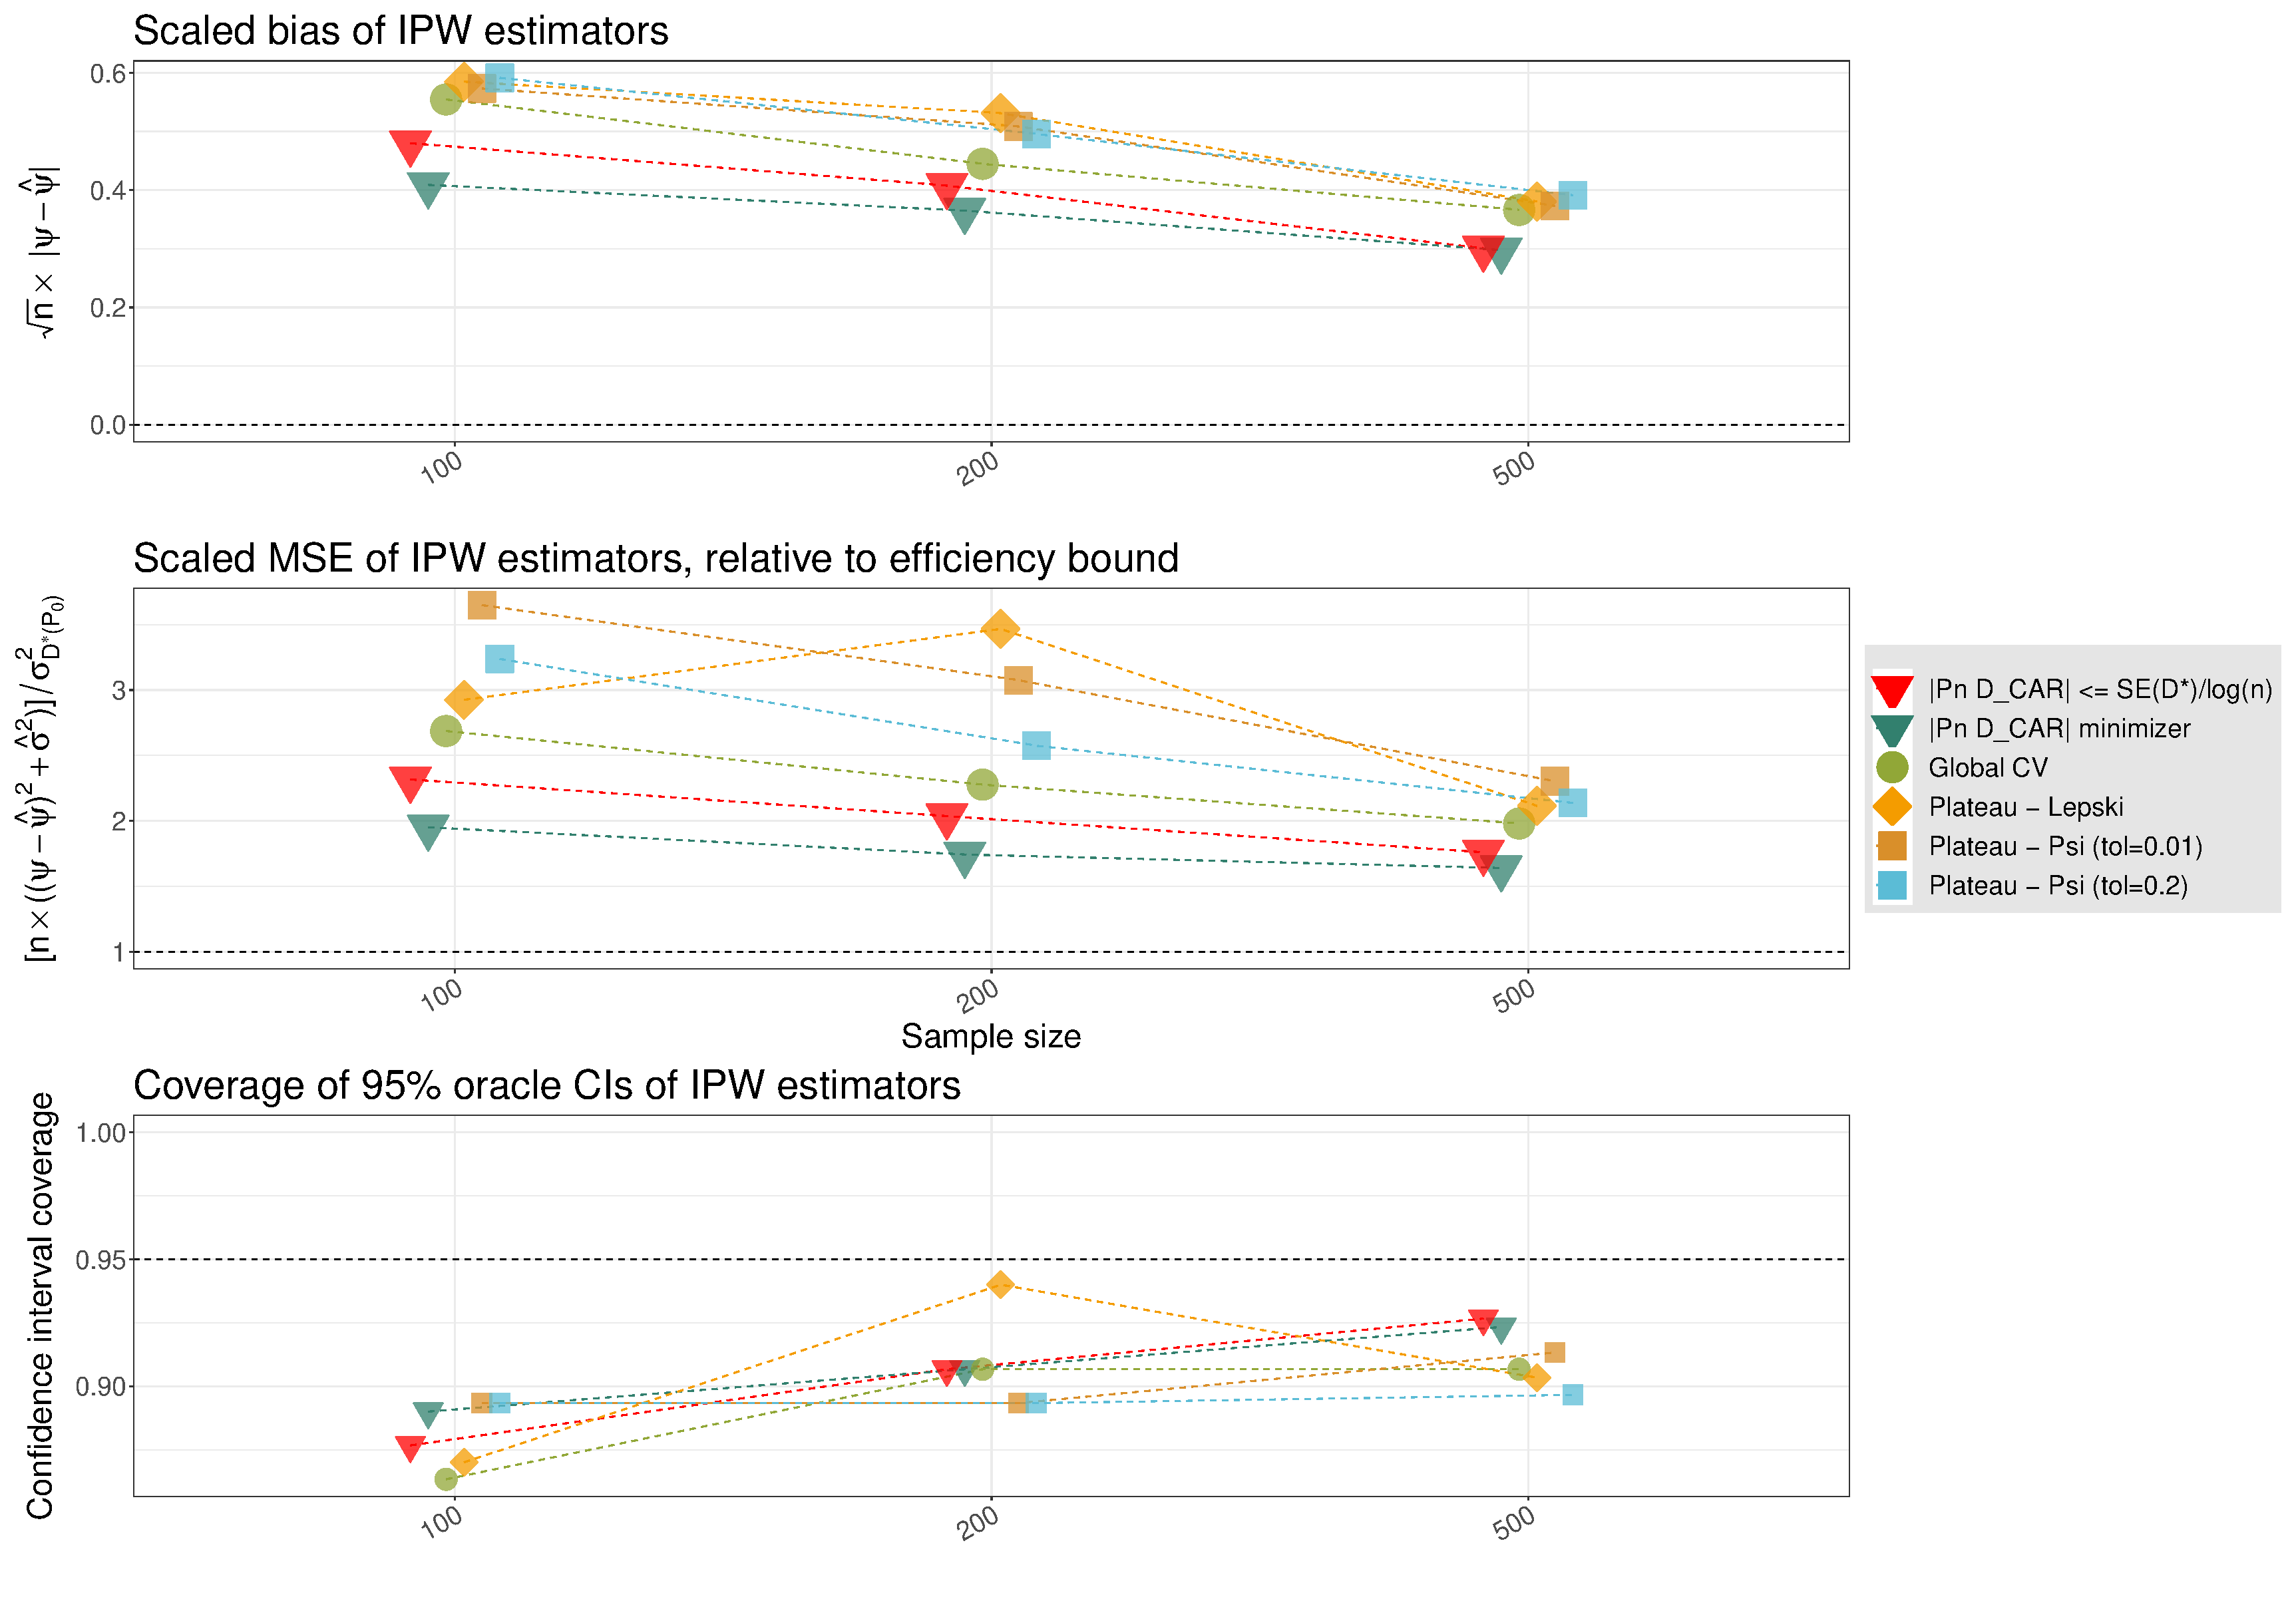
\includegraphics[scale=0.28]{dgp1a_npipw_all_paneled_Qn_hal}
  \caption{Numerical comparisons of nonparametric IPW estimator variants of
     $\psi_{0,\delta}$ for $A \sim \text{Normal}(\mu = f(W), \sigma^2 = k)$.}
  \label{fig:dgp1a_npipw}
\end{figure}
Inspection of Figure~\ref{fig:dgp1a_npipw} reveals generally acceptable
performance of all of our IPW estimators, with bias of $0.06$ and $0.04$ in the
worst and best cases, respectively, at $n=100$; this performance improves to a
bias of $0.018$ in the worst case and of $0.013$ in the best case at $n=500$. In
terms of bias, our IPW estimators using targeted undersmoothing outperform the
other variants uniformly across sample sizes, though the difference is not great
between the best and worst case biases. Considering the scaled MSE, the IPW
estimators using targeted undersmoothing once again dominate the others
uniformly across sample sizes. Notably, in terms of this performance measure,
the IPW estimator utilizing the cross-validation selector outperforms those
using agnostic undersmoothing. This is a surprising finding since
cross-validation chooses the optimal estimator of $g_{0,A}$, not necessarily
that of $\psi_{0,\delta}$; moreover, this relatively good performance suggests
that even cross-validation may make for a reasonably reliable strategy in
constructing nonparametric IPW estimators of $\psi_{0,\delta}$. With respect to
the empirical coverage of oracle confidence intervals, none of the candidate
IPW estimators succeed in attaining the nominal rate, though this is consistent
with the prior observation that none of the estimators are perfectly unbiased at
any of the sample sizes. Altogether, the results of this experiment suggest that
targeted undersmoothing of the HAL generalized propensity score estimator can be
used to construct nonparametric IPW estimators with reasonably good, though not
excellent, asymptotic consistency and efficiency.

\subsection{Simulation \#2: Treatment Mechanism with Unequal Mean and Variance
Dependent on Baseline}\label{hese_sim_norm}

The next scenario is a modification of the previous, in which the form of the
treatment mechanism is kept fixed to a normal distribution, though the mean and
variance are now modified to both be functions of a subset of the baseline
covariates $\{W_1, W_2\}$; $W_3$ has no impact on the treatment mechanism but
does appear in the outcome mechanism, whose forms is a function of the treatment
$A$ and all baseline covariates. Perhaps significantly, the form of the
treatment mechanism in this scenario demands accurate estimation of both the
location and scale parameters of the normal distribution; moreover, the
heteroscedasticity with respect to the baseline covariates complicates accurate
estimation of the conditional density $g_{0,A}$ relative to the form of the
treatment mechanism in the prior scenario. While the form of the outcome
mechanism differs from that in the previous scenario, we again do not expect its
form to affect the construction of our IPW estimators much. The treatment
mechanism takes the form $A \mid W \sim \text{Normal}\left(\mu = W_1 + 2 W_2
- 2 \cdot (1 - W_1) \cdot W_2, \sigma^2 = 2 W_1 + 0.5 (1 - W_1) + W_2 \right)$,
while the outcome mechanism is $Y \mid A, W \sim \text{Bernoulli}\left(p
= \text{expit}(5 (A - 2) + W_1 + 3 W_2^4 - 2 W_3 - \allowbreak 4 (1 - W_1)
W_2)\right)$.

We summarize the performance of our proposed IPW estimators in terms estimation
of $\psi_{0,\delta}$ across the $300$ simulation experiments in
Figure~\ref{fig:dgp1b_npipw}.
\begin{figure}[H]
  \centering
  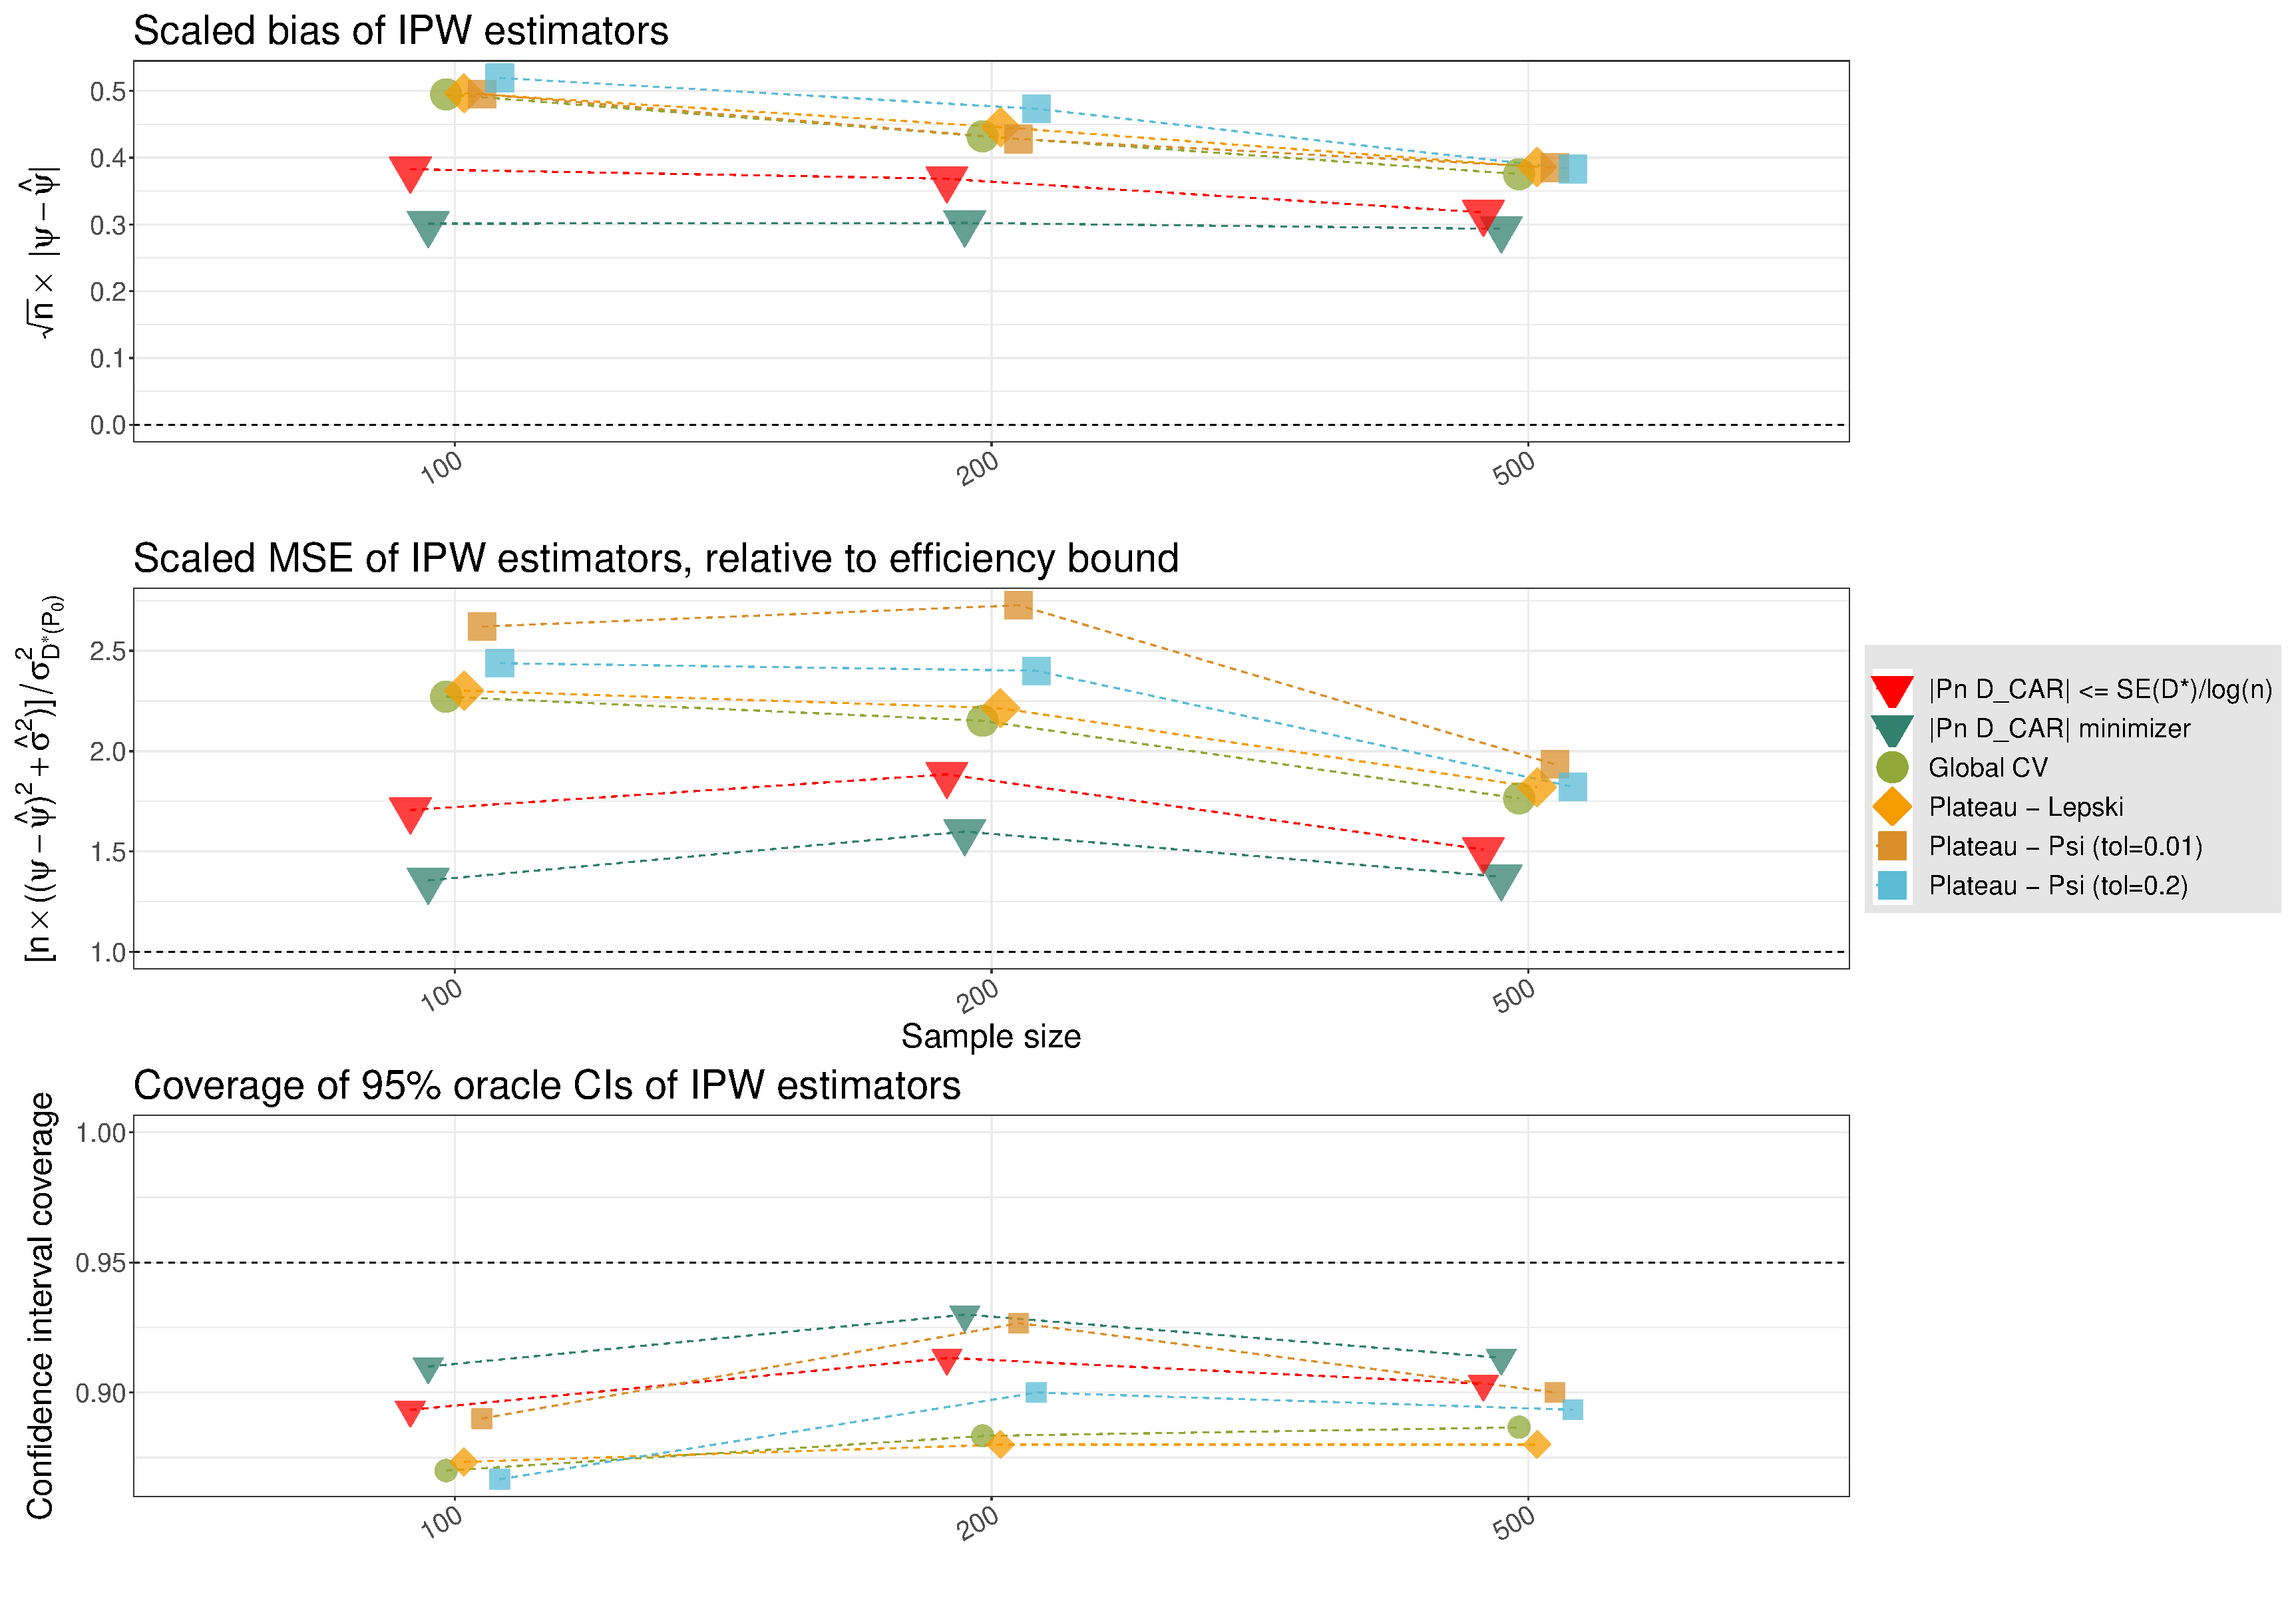
\includegraphics[scale=0.28]{dgp1b_npipw_all_paneled_Qn_hal}
  \caption{Numerical comparisons of nonparametric IPW estimator variants of
     $\psi_{0,\delta}$ for $A \sim \text{Normal}(\mu = f_1(W), \sigma^2 =
     f_2(W))$.}
  \label{fig:dgp1b_npipw}
\end{figure}
Upon examination, Figure~\ref{fig:dgp1b_npipw} reveals relative performance
measures of the IPW estimators very similar to that observed in the prior
scenario. In particular, the IPW estimators constructed based on targeted
undersmoothing outperform all of the other candidates in terms of both bias and
efficiency. In terms of bias, all estimators again achieve acceptable levels of
performance: at $n=100$, bias is $0.052$ in the worst case and $0.03$ in the
best case, while at $n=500$, the same metrics are $0.018$ and $0.013$,
respectively. Turning now to efficiency, none of the estimators achieve the
efficiency bound of the model at the examined sample sizes, though the
decreasing trajectory of their scaled MSEs suggests promising performance at
larger sample sizes. In this scenario, the IPW estimator based on the
cross-validation selector performs similarly to those based on agnostic
undersmoothing. As none of our proposed IPW estimators is perfectly unbiased,
the constructed oracle confidence intervals fail to attain the nominal coverage
rate, consistent with expectations. The results of this experiment echo those of
the first --- our IPW estimators utilizing targeted undersmoothing outperform
the others, though not considerably in any metric.

\subsection{Simulation \#3: Treatment Mechanism with Equal Mean and Variance
Dependent on Baseline}\label{hese_sim_poisson}

We next consider our final experimental scenario, which breaks from the
preceding two examples by basing the form of the treatment mechanism on
a Poisson distribution, so that the mean and variance are both equally impacted
by the relevant baseline covariates. As with the example immediately prior, the
treatment mechanism is a function of a subset of the baseline covariates
$\{W_1, W_2\}$, with $W_3$ only impacting the outcome mechanism. As with our
prior experiments, the form of the outcome mechanism is not expected to impact
our proposed IPW estimators, since estimation of the outcome mechanism only
plays a role in our targeted undersmoothing selection procedures. We note that
the form of the treatment mechanism results in $A$ taking on discrete values in
a fairly large range, unlike the continuous-valued observations that result from
the normal distribution appearing in the prior examples; this treatment
mechanism's form is possibly more compatible with the generalized propensity
score estimator of Algorithm~\ref{alg:pooled_haz_dens}, which utilize
discretization of $A$ for estimation of the conditional density. For this
scenario, the treatment mechanism takes the form $A \mid W \sim
\text{Poisson}\left(\lambda = (1 - W_1) + 0.25 W_2^3 + 2 W_1 W_2 + 4\right)$ and
outcome mechanism is of the form $Y \mid A, W \sim \text{Bernoulli}\left(p
= \text{expit}(A + 2 (1 - W_1) + 0.5 W_2 + 0.5 W_3 + 2 W_1 W_2 - 7)\right)$.

Numerical evaluation of the performance of our proposed IPW estimators of
$\psi_{0,\delta}$ across the $300$ simulation experiments is summarized in
Figure~\ref{fig:dgp2a_npipw}.
\begin{figure}[H]
  \centering
  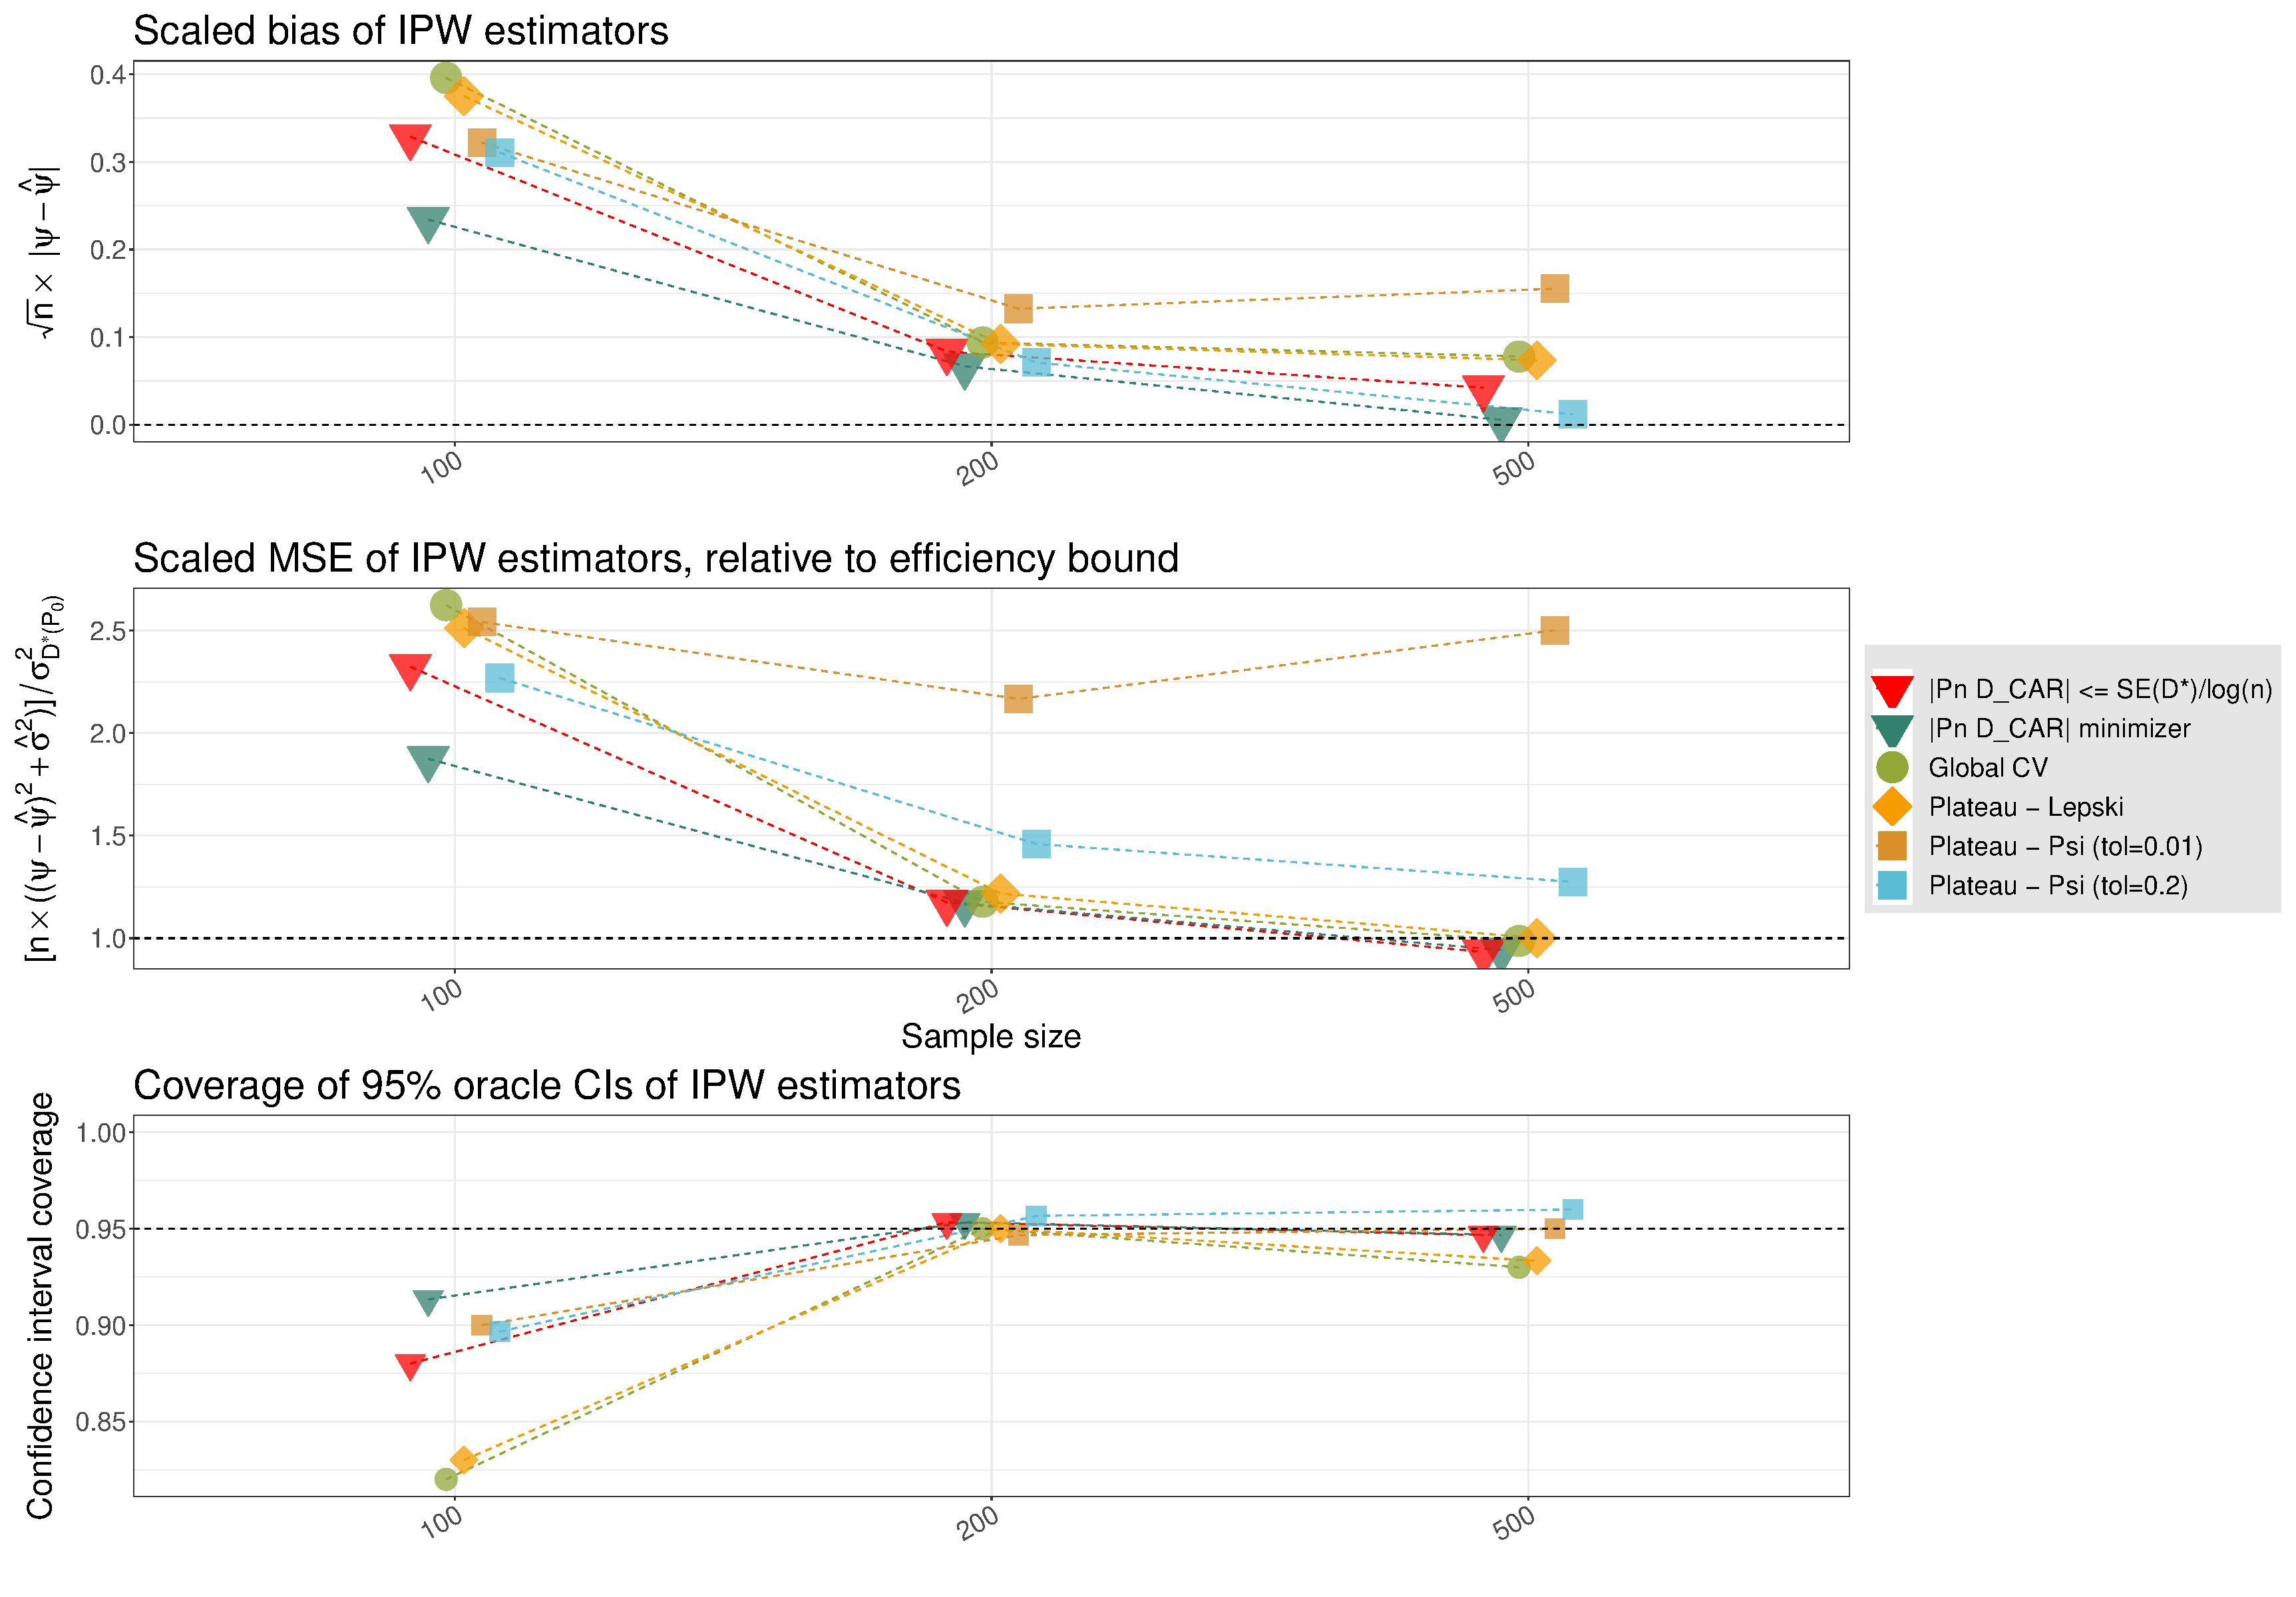
\includegraphics[scale=0.28]{dgp2a_npipw_all_paneled_Qn_hal}
  \caption{Numerical comparisons of nonparametric IPW estimator variants of
       $\psi_{0,\delta}$ for $A \sim \text{Poisson}(\lambda = f(W))$.}
  \label{fig:dgp2a_npipw}
\end{figure}
Figure~\ref{fig:dgp2a_npipw} reveals the best performance of our proposed IPW
estimators encountered thus far. In this setting, the IPW estimator variants
using targeted undersmoothing outperform the others only at the smallest sample
size --- that is, at $n=100$, the IPW estimator based on minimization of the
EIF term arising from Lemma~\ref{lemma:dcar} achieves the lowest bias and best
efficiency. By $n=500$, most estimator variants are nearly unbiased, with the
best performing being IPW estimators minimizing $\lvert P_n D_\text{DCAR}
\rvert$ via targeted undersmoothing and the less restrictive ($\tau = 0.2$)
agnostic undersmoothing selector based on equation~\eqref{eqn:plateau_psi_rel}.
In terms of efficiency, all candidates but the IPW estimators constructed from
agnostic undersmoothing based on equation~\eqref{eqn:plateau_psi_rel} succeed in
achieving the efficiency bound, an excellent level of performance. Notably, even
the IPW estimator based on the cross-validation selector succeeds in this
challenging endeavor, suggesting that it exhibits variance relatively improved
beyond that of the other candidates, on account of the fact that it is not
similarly unbiased. Unlike the prior scenarios, the oracle confidence intervals
of all candidate IPW estimators attain the nominal coverage rate by $n=200$,
with similar performance at $n=500$. Importantly, the excellent performance of
all of the estimator candidates with respect to this metric suggests that all
are capable of providing reliably good performance and that relative performance
differences across the candidates may be better ascribed to variance estimation
than to point estimation, the latter of which is our principal focus. Though the
previously considered scenarios were not discouraging, the results of this set
of experiments are quite positive, suggesting that at least a few variants of
our proposed IPW estimators may successfully applied to reliably and efficiently
estimate $\psi_{0,\delta}$.

%%%%%%%%%%%%%%%%%%%%%%%%%%%%%%%%%%%%%%%%%%%%%%%%%%%%%%%%%%%%%%%%%%%%%%%%%%%%%%%
\section{Discussion}\label{discuss}

The generalized propensity score is a central object in evaluating the causal
effects of continuous treatments. While stochastic interventions provide
a framework for identifying causal effects of realistic interventions, their
formulation too depends on the generalized propensity score. Accordingly,
flexible estimators of this key nuisance quantity, relying on recent
developments in nonparametric regression, are poised to play important roles in
developing consistent and efficient estimators of the causal effects of
stochastic interventions. We have provided an initial examination of the role of
a flexible regression algorithm, the recently developed highly adaptive lasso
estimator, in developing conditional density estimators with favorable
theoretical properties. Building on these contributions, we formulated
nonparametric IPW estimators of the causal effects of stochastic interventions,
previously absent from the causal inference literature. To further improve our
IPW estimators, we outlined several selection procedures, to be used in tandem
with undersmoothing of our proposed HAL-based conditional density estimators, to
allow these novel IPW estimators to achieve the nonparametric efficiency bound,
a property previously attainable by doubly robust estimators. In numerical
experiments, we examined the relative performance our nonparametric IPW
estimators, demonstrating their capability to achieve low bias and attain the
efficiency bound in some examples. Several avenues for future investigation
remain, including potential improvements to doubly robust estimators that
incorporate undersmoothing of the generalized propensity score, which may
exhibit higher-order types of efficiency or make doubly robust
inference~\citep[e.g.,][]{benkeser2017doubly} possible, and the extension of our
nonparametric IPW estimators to more complex settings in which stochastic
interventions have proven useful, including causal mediation
analysis~\citep[e.g.,][]{diaz2020causal}.

\chapter{Correcting for Biased Sampling}

The advent and subsequent widespread availability of preventive vaccines has
altered the course of public health over the past century. Despite this success,
effective vaccines to prevent many high-burden diseases, including HIV, have
been slow to develop. Vaccine development can be aided by the identification of
immune response markers that serve as effective surrogates for clinically
significant infection or disease endpoints. However, measuring immune response
marker activity is often costly, which has motivated the usage of two-phase
sampling for immune response evaluation in clinical trials of preventive
vaccines. In such trials, the measurement of immunological markers is performed
on a subset of trial participants, where enrollment in this second phase is
potentially contingent on the observed study outcome and other participant-level
information. We propose nonparametric methodology for efficiently estimating
a counterfactual parameter that quantifies the impact of a given immune response
marker on the subsequent probability of infection. Along the way, we fill in
theoretical gaps pertaining to the asymptotic behavior of nonparametric
efficient estimators in the context of two-phase sampling, including a multiple
robustness property enjoyed by our estimators. Techniques for constructing
confidence intervals and hypothesis tests are presented, and an open source
software implementation of the methodology, the \texttt{txshift} \texttt{R}
package, is introduced. We illustrate the proposed techniques using data from
a recent preventive HIV vaccine efficacy trial.

\section{Introduction}\label{intro}

Ascertaining the population-level causal effects of exposures is a common goal
in scientific research. Such effects can be formulated via summaries of the
distribution of \emph{counterfactual random variables}, which describe the
values a measurement would have taken if a particular level of exposure were
assigned to the unit. Often, the exposure of interest is continuous-valued ---
for example, the dose of a drug or level of an immune response marker induced by
a vaccine. We consider the latter in the context of a phase IIb trial of
a vaccine to prevent infection by human immunodeficiency virus (HIV), the HIV
Vaccine Trials Network's (HVTN) 505 efficacy trial~\citep{hammer2013efficacy}.
A key secondary objective of the trial was to evaluate the role of
vaccine-induced immune responses in generating protective efficacy against HIV
infection~\citep{janes2017higher}. Identification of immune response markers
\textit{causally} related to protection is critical both for understanding of
the biological mechanisms of a vaccine and for guiding the development of future
vaccines.

To study such relationships, it is natural to consider a dose-response curve
that summarizes vaccinated participants' risk of HIV infection as a function of
a particular immune response marker. A causal formulation of such
a dose-response analysis would consider a (possibly infinite) collection of
counterfactual outcomes, each representing the HIV infection risk that would
have been observed if all individuals' immune responses had been set to
a particular level. Studying how the proportion of infected individuals varies
as a function of the level of an immune response marker could provide insights
into causal mechanisms underlying the vaccine's effects. Unfortunately, several
difficulties arise when considering such a dose-response approach. Nonparametric
estimation and inference on the causal dose-response curve is challenging and
requires non-standard techniques (e.g., \citet{kennedy2017nonparametric}). More
importantly, this approach may require consideration of counterfactual variables
that are scientifically unrealistic. Namely, it may be impossible to imagine
a world where every vaccinated participant exhibits high immune responses,
simply due to phenotypic variability of participants' immune systems. This calls
into question the validity of counterfactual dose-response analysis strategies
that evaluate the effects of immune response markers.

An alternative framework for assessing effects of continuous-valued exposures
involves counterfactual outcomes resulting from \textit{stochastic}
interventions~\citep{diaz2012population, haneuse2013estimation}. Whereas static
interventions set the same level of an exposure to all units, stochastic
interventions instead set exposure level equal to a random draw from
a particular distribution. This provides a more flexible approach for defining
counterfactual random variables. Indeed, static interventions are a special case
of stochastic interventions in which the intervention mechanism is drawn from
a degenerate distribution with point mass on a single value. To define
meaningful counterfactuals, care must be taken in defining the distribution from
which the exposure is drawn. One strategy is to draw from a modified version of
the true exposure distribution --- the \textit{natural distribution} of exposure
under no intervention. For example, one may consider drawing immune response
markers from a distribution similar to the naturally observed post-vaccination
distribution of immune response markers \textit{but} that has been shifted
upwards (or downwards) for some or all participants. Counterfactuals defined by
such interventions may be better aligned with plausible future interventions,
such as refinements of the current vaccine that provide improved immune
responses. Evaluating the population-level risk of HIV infection under such
interventions is useful for several reasons. Firstly, this measure of risk
provides a relevant mechanism by which to rank-order immune response markers by
their importance for HIV infection risk. Such information could be used in
a future phase 2a trial of a refined candidate HIV vaccine to define  go/no-go
criteria based on immune response marker endpoints for advancing the vaccine to
an efficacy trial. Relatedly, the risk measure may be useful for ``transport
formulas'' that predict vaccine efficacy in new settings different from that in
the original efficacy trial~\citep{pearl2014external}.
%Such information could be used in defining go/no-go criteria in future
%early-phase HIV vaccine development pipelines. Secondly, the risk measure may
%also provide a way to predict next-generation vaccine efficacy based on the
%induced immune response profile, elucidating whether the immune response induced
%by a candidate vaccine is sufficiently promising to advance it to the clinical
%trial stage.
%\vdl{Under this strategy, the post-intervention distribution implied by
%a stochastic intervention is a modification of the true exposure distribution}.

%\db{The next two are crucial paragraphs to get right. We need to clarify what
%our contributions are over those of Sherri/Mark and Ivan/Mark.}

The above highlights the need for methodology to identify and estimate
population-level causal effects of stochastic interventions; recent work has
provided several candidate approaches~\citep{diaz2012population,
haneuse2013estimation}. These works show conditions for the identification and
detail several estimators of parameters of distributions of counterfactuals
defined by stochastic interventions. However, these approaches are not directly
applicable to studies like HVTN 505 trial, where a two-phase, case-cohort
sampling design was used to measure participants' immune responses. Under this
design, \textit{all} vaccine recipients diagnosed with HIV-1 infection (i.e.,
``cases'') had their post-vaccination immune responses measured, while only
a \textit{random sample} of HIV-uninfected vaccine recipients had immune
responses measured~\citep{janes2017higher}. This sampling design complicates the
estimation of causal effects, as the cohort definition depends on
post-randomization data, namely whether a participant was infected.
\citet{rose2011targeted2sd}, among others, discuss strategies for efficient
estimation under two-phase sampling designs, emphasizing an inverse probability
of censoring weighted modification that may be coupled with targeted minimum
loss estimation to account for study design. Their approach yields an
asymptotically linear estimator so long as the probability of inclusion in the
second-phase sample is known by design or estimable via maximum likelihood. This
latter requirement precludes usage of their proposed estimators in situations
where, for example, sampling probabilities are unknown and may depend on
continuous-valued covariates. While the term ``two-phase sampling'' has
traditionally been used to refer to outcome-dependent Bernoulli or
without-replacement sampling based on discrete covariates, recent efforts have
extended the concept to the usage of continuous-valued covariates in
constructing second-phase samples~\citep[e.g.,][]{gilbert2014optimal}.
\citet{rose2011targeted2sd} suggested a more complicated procedure that could be
appropriate in such settings, but it has neither been evaluated in simulation
nor data analysis.

In the present work, we develop estimators of the mean counterfactual outcome
under a stochastic intervention when the exposure is measured via two-phase
sampling. We provide several contributions to literatures on two-phase sampling
and stochastic interventions. To the former, we (i) formalize assumptions needed
for efficient nonparametric inference under two-phase sampling; (ii)
characterize a multiple robustness of the estimators; and (iii) provide the
first comparison of the practical performance of these estimators. Our
contributions to the literature on stochastic interventions are (i) a novel
estimator of a conditional density that is valid under two-phase sampling, while
achieving a fast convergence rate, a crucial development for generating
efficient estimators of the mean counterfactual; and (ii) an extension of
nonparametric inference on mean counterfactuals under stochastic interventions
using projections onto nonparametric working marginal structural models.
Finally, we provide open source R packages,
\texttt{txshift}~\citep{hejazi2020txshift, hejazi2020txshift-joss} and
\texttt{haldensify}~\citep{hejazi2020haldensify} that implement of our proposed
estimators.

\section{Preliminaries and Background}\label{background}

\subsection{Notation, data, and target parameter}\label{parameter}

Consider data generated by typical cohort sampling represented by the random
variable $X = (W, A, Y)$, where $W \in \mathcal{W}$ is a vector of baseline
covariates, $A \in \mathcal{A}$ a real-valued exposure, and $Y \in \mathcal{Y}$
an outcome of interest. Initially, we assume access to $n$ independent copies of
$X$, using $P_0^X$ to denote the distribution of $X$. We assume a nonparametric
statistical model $\mathcal{M}^X$ for $P_0^X$. We denote by $q_{0, Y}$ the
conditional density of $Y$ given $\{A, W\}$ with respect to some dominating
measure, $q_{0, A}$ the conditional density of $A$ given $W$ with respect to
dominating measure $\mu$, and $q_{0, W}$ the density of $W$ with respect to
dominating measure $\nu$. We use $p_0^X$ to denote the density of $X$ with
respect to the product measure. This density evaluated on a typical observation
$x$ may be expressed $p_0^X(x) = q_{0,Y}(y \mid A = a, W = w) q_{0,A}(a \mid
W = w) q_{0,W}(w)$.
%\note[David]{Ivan still calls density of $A \mid W$ $g$, but I think maybe we
%want to use $q$ since it is involved in the computation of the parameter. We
%can use $g$ then for the probability that $\Delta = 1 \mid Y, W$}

To define a counterfactual quantity of interest, we introduce a nonparametric
structural equation model (NPSEM)~\citep{pearl2000causality}, which assumes $X$
is generated by the following system of structural equations: $ W = f_W(U_W);
A = f_A(W, U_A); Y = f_Y(A, W, U_Y)$. Here, $f$ are deterministic functions and
$\{U_W, U_A, U_Y\}$ are exogenous random variables such that $U_A \perp U_Y$ and
either $U_W \perp U_Y$ or $U_W \perp U_A$, which establishes that conditioning
on $W$ is sufficient to control confounding of $A$ and $Y$.

The NPSEM parameterizes $p_0^X$ in terms of the distribution of the random
variables $(X, U)$ and implies a model for the distribution of counterfactual
random variables generated by interventions on the data-generating process. For
example, a \textit{static intervention} replaces $f_A$ with a real number $a$.
A \textit{stochastic intervention} replaces the value $A$ would naturally assume
with a draw from a post-intervention distribution $\tilde{q}_{0,A}(\cdot \mid
W)$, where the zero subscript is included to emphasize that $\tilde{q}_{0,A}$
may depend on $P_0^X$. A static intervention may be viewed as a stochastic
intervention where $\tilde{q}_{0,A}(\cdot \mid W)$ places all mass on a single
point. \citet{diaz2012population} described a stochastic intervention that draws
$A$ from a distribution such that for a real number $a$ $\tilde{q}_{0,A}(a \mid
W) = q_{0,A}(a - \delta(W) \mid W)$ for a user-supplied shifting function
$\delta(W)$. \citet{haneuse2013estimation} showed that estimating the effect of
this intervention is equivalent with that of an intervention that modifies the
value $A$ would naturally assume according to a regime $d(A,W)$. Importantly,
the regime $d(A,W)$ may depend on both the covariates $W$ and the exposure level
$A$ that would be assigned in the absence of the regime; consequently, this has
been termed a \textit{modified treatment policy} (MTP). Both
\citet{haneuse2013estimation} and \citet{diaz2018stochastic} considered an MTP
of the form $d(a,w) = a + \delta(w)$ for $\delta(w) = \gamma \in \R$ if $a
+ \gamma \leq u(w)$ and $d(a,w) = a$ if $a + \gamma > u(w)$, where $u(w)$ is the
maximum value in the support of $q_{0,A}(\cdot \mid W = w)$. This intervention
generates a counterfactual random variable $Y_{A + \delta(W)} \coloneqq f_Y(A
+ \delta(W), W, U_Y)$ whose distribution we denote $P_0^{\delta}$; we seek to
estimate $\psi_{0, \delta} \coloneqq \E_{P_0^{\delta}} \{ Y_{A + \delta(W)} \}$,
the mean of this counterfactual outcome.

%A detailed discussion of the similarities and differences between the approaches
%of \citet{diaz2012population} and \citet{haneuse2013estimation}, primarily in
%terms of their interpretation and identification, is provided by
%\citet{young2014identification}.

In the context of HVTN 505, this parameter corresponds to the counterfactual
one-year risk of HIV-1 infection had immune response markers of vaccinated
participants been increased by $\gamma$ units relative to the level induced by
the current vaccine. This quantity may reflect risk of infection under
a next-generation HIV vaccine with improved immunogenicity relative to the
vaccine evaluated in HVTN 505. While the magnitude of shifting could generally
be allowed to vary with $W$, we focus on an intervention that uniformly shifts
all participants' immune responses by $\gamma$, that is, $d(a,w) = a + \gamma$
for all $a$. Note that for HVTN 505, the parameter of interest is defined only
for the vaccine group, making $A$ a post-vaccination marker measuring an
HIV-specific immune response. Importantly, it is not conceivable to define the
target parameter for placebo recipients since only HIV-negative participants are
enrolled in the trial and $A$ is only defined if measured prior to HIV
infection; consequently, all relevant placebo recipients have value zero for the
marker $A$, and it is not meaningful to apply $d(a,w)$ to shift the distribution
of $A$.

Analysis of HVTN 505 is complicated by its two-phase design, a technique
commonly used for sampling in vaccine efficacy trials. In this sampling scheme,
$X$ is not observed all participants. Instead, we observe $O = (W, C, C A, Y)
\sim P_0$, where $C$ is an indicator that an observation is included in the
second-phase sample; $C_i = 1$ if $A$ is measured on the $i^{\text{th}}$
observation and $C_i = 0$ otherwise. By convention, $C A$ denotes that
unobserved values of $A$ are set to zero; this arbitrary labeling has no impact
on subsequent developments. For each $w$ and $y$ we define $g_{0, C}(y, w)
\coloneqq \prob(C = 1 \mid Y = y, W = w)$, allowing that the probability of
inclusion in the second-phase sample can depend on $W$ and $Y$. Consequently,
the model for $P_0$ can be expressed as $\M = \{P_{P^X, g_C}: P^X \in \M^X,
g_C\}$, that is, $P_0$ is implied by the pair $\{P^X_0, g_{0, C}\}$. For
example, in HVTN 505 all infected participants with samples available for marker
measurement at week 28 had immune responses measured, i.e., $g_{0,C}(1,w) = 1$
for all $w$; however, only a subset of non-infected participants had immune
responses measured. We will assume access to an i.i.d.~sample $O_1, \ldots,
O_n$, denoting its empirical distribution by $P_n$. We develop efficient
nonparametric estimators of $\psi_{0,\delta}$ based on these data.

%\subsection{Stochastic intervention policies}\label{stochastic}

%To formalize a stochastic intervention, consider an intervention shift function
%$d(A, W)$ that arbitrarily shifts the natural value of the intervention $a$ by
%$\delta$ units. For example, consider a simple additive intervention shift
%function $d(A, W) = A + \delta$, for $A \in \mathcal{A}$ and $\delta \in
%\mathcal{A}$ that shifts the natural value of the intervention $a$ so that the
%counterfactual intervention quantity is $a + \delta$. Such an intervention
%shift function was first proposed by \cite{diaz2012population,
%diaz2018stochastic}, who define this additive intervention shift function as
%follows \begin{equation}\label{shift_intervention} d(a, w) = \begin{cases} a +
%\delta, & a + \delta < u(w) \\ a, & \text{otherwise} \end{cases},
%\end{equation} where $(l(w), u(w))$ defines the support of the conditional
%density of $A$ given $W = w$. This formulation of $d(A, W)$ is noteworthy in
%that it protects against violations of the assumption of positivity, since the
%shift value $\delta$ is \textit{not} applied to an observed value of the
%intervention $a$ when the resultant counterfactual quantity $a + \delta$ would
%lie outside of the support of the conditional density $q_{0, A}(A \mid W)$ in
%the observed data.

%Using $d(A,W)$ as defined above, \cite{diaz2012population} show that the causal
%quantity of interest $\E Y_{d(A, W)}$ may be identified from data based on the
%full data unit $X$: \begin{align*}\label{eqn:identification2012} \E Y_{d(A, W)}
%&= \int_{a \in \mathcal{A}} \int_{w \in \mathcal{W}} \E (Y \mid A = d(a, w), W
%= w) q_{0, A}^X(a \mid W = w) q_{0, W}^X(w) dv(a, w) \\ &= \E_{p_0^X} \{
%\overline{Q}(d(A, W), W) \}, \end{align*} where $\overline{Q}$ denotes the
%conditional distribution of $Y$ with respect to the density $p_0^X$, which then
%allows the statistical parameter of interest to be defined as $\psi_{0, d} =
%\psi(p_0^X) = \E_{p_0^X}\{\overline{Q}(d(A,W), W)$, as given above. In the
%remainder of their work, \cite{diaz2012population} discuss a relevant postivity
%assumption; provide an efficient influence function (EIF) with respect to a
%nonparametric model $\M$, which we reproduce as eqn.~\ref{eqn:eif_full} in
%Section \ref{target}; and use this EIF as an estimating equation to propose a
%targeted minimum loss-based (TML) estimator of $\psi_{0,d}$. In later work, an
%improved algorithm for computing this TML estimator more easily was developed
%\citep{diaz2018stochastic}.

%Building on this work, \cite{haneuse2013estimation} discuss an alternative
%respresentations of stochastic interventions based on a decomposition of the
%intervention density, showing that such intervention regimes may be viewed as
%imposing a change to the structural equation $f_A$ in the NPSEM such that $f_A$
%is removed and the value of $A$ is drawn from a shifted intervention density.
%In particular, this implies that stochastic interventions may be viewed as a
%change in either the subject-specific intervention value or in the
%probabilistic mechanism used to assign the intervention. In spite of these two
%definitions, \cite{young2014identification} show that the population
%distribution of the intervention is the same under both types of stochastic
%interventions; thus, the approaches of both \cite{diaz2012population} and
%\cite{haneuse2013estimation} yield the same counterfactual distribution of the
%outcome and so the same value of the parameter of interest.

%\subsection{Two-phase sampling}\label{sampling}

%There is a rich literature considering the use of two-phase sampling designs
%and the potential problems for estimation and inference that such designs
%impose. In the context of targeted minimum loss-based estimation,
%\cite{rose2011targeted2sd} propose the use of inverse probability of censoring
%(IPC) weights to augment TML estimators. Considering the observed data unit $O
%= (W, \Delta, \Delta A, Y)$, introduced in Section \ref{parameter},
%\cite{rose2011targeted2sd} develop theoretical results showing that a TML
%estimator may be constructed for a target parameter --- in our case,
%$\psi_{0,d}$ --- of the full data unit $X$ by considering the use of IPC
%weights based on the sampling mechanism $g_{0, \Delta}$. In order to develop an
%augmented TML estimator based on such weights, letting $g_{n, \Delta}$ denote
%an estimator of $g_{0, \Delta}$, IPC weights of the desired form may be
%constructed as $\frac{\Delta_i}{g_{n, \Delta}(Y_i, W_i)}$ for all observed data
%units $O_i$, $i: 1, \ldots, n$; moreover, in order to construct unbiased and
%efficient TML estimators, such weights may be applied either to (i) an
%appropriate loss function or (ii) the efficient influence function of an
%estimator with respect to a nonparametric model \citep{rose2011targeted2sd}. In
%spite of the apparent utility of such an approach, there are several important
%limitations that must be overcome before this technique may be applied to
%complex studies like HVTN 505.

%In many real-world applications, including HVTN 505, the sampling mechanism of
%the two-phase design may indiscriminately incorporate a variety of covariates.
%A key advantage of the IPCW-TML estimator of \cite{rose2011targeted2sd} is that
%the augmented estimator readily inherits key properties of the full data TML
%estimator, such as double robustness --- unfortunately, this inheritance
%property necessitates that $g_{n, \Delta}$ be a consistent estimator of the
%true (and unknown) sampling mechanism $g_{0, \Delta}$. To obtain consistent
%estimates in settings involving complex sampling, it is tempting to consider
%the use of a nonparametric estimator for $g_{n, \Delta}$; however, this is only
%recommended in the case that covariates $\{Y, W\}$ used in the sampling
%mechanism are discrete (with finite support). This is an important limitation
%that precludes the use of data-adaptive and nonparametric regression approaches
%in the estimation of the sampling mechanism. What's more, when considering a
%full data model that is nonparametric, \cite{rose2011targeted2sd} demonstrate
%that the IPCW-TML estimator solves the full data efficient influence function
%estimating equation, even when the sampling mechanism is estimated
%nonparametrically.  Unfortunately, this again requires that the covariates
%considered in the sampling mechanism $\{Y, W\}$ be discrete.

%In the sequel, we propose an approach that allows for the sampling mechanism to
%be estimated nonparametrically, without requiring discreteness of $\{Y, W\}$,
%and build off of \cite{diaz2012population, diaz2018stochastic} to construct a
%semiparametric-efficient estimator that displays multiple robustness under a
%two-phase sampling design.

\subsection{Identifying the counterfactual mean under a stochastic
intervention}\label{stoch_lit}

\citet{diaz2012population} established that $\psi_{0,\delta}$ is
identified by
\begin{align}\label{eqn:identification2012}
  \psi_{0,\delta} &= \int_{\mathcal{W}} \int_{\mathcal{A}}
  \overline{Q}_{0,Y}(a + \delta(w), w) q_{0, A}(a \mid W = w)
  q_{0, W}(w) d\mu(a)d\nu(w)
  %\E_{P_0^X} \{Y \mid A = \delta(a, w), W = w\} q_{0, A}^X(a \mid W = w)
  %q_{0, W}^X(w) d\mu(a)d\nu(w) \ .
\end{align}
where $\overline{Q}_{0,Y}(a,w) \coloneqq \E_{P_0^X}[Y \mid A = a, W = w]$, the
conditional mean of $Y$ given $A = a$ and $W = w$, as implied by $P_0^X$. Let
$Y_{a_i + \delta(w_i)}$ denote the outcome that would have been observed had the
observed exposure been, possibly counter-to-fact, set to $a_i + \delta(w_i)$;
identification of the causal estimand of interest by
equation~(\ref{eqn:identification2012}) is established under several
assumptions: consistency ($Y_{i, a_i + \delta(w_i)} = Y_i$ in the event $A_i
= a_i + \delta(w_i)$, for $i = 1, \ldots, n$); no interference ($Y_{i, a_i
+ \delta(w_i)}$ does not depend on $a_j + \delta(w_j)$ for $i \neq j$ and $i
= 1, \ldots, n$); no unmeasured confounding ($A_i \indep Y_{i, a_i
+ \delta(w_i)} \mid W = w_i$, for $i = 1, \ldots, n$); and positivity ($a_i \in
\mathcal{A} \implies a_i + \delta(w_i) \in \mathcal{A} \mid W = w_i$ for all $w
\in \mathcal{W}$ and $i = 1, \ldots n$). Importantly, even when these untestable
assumptions go unsatisfied, the statistical parameter appearing in
equation~(\ref{eqn:identification2012}) has a straightforward interpretation: it
is the adjusted mean of the outcome $Y$ under the contrast $A + \delta(W)$,
marginalizing over strata of potential baseline confounders
$W$~\citep{diaz2012population, vdl2011targeted}.

The positivity assumption required to establish
equation~(\ref{eqn:identification2012}) is unlike that required for static or
dynamic interventions. In particular, it does not require that the
post-intervention exposure density place mass across all strata defined by $W$.
Instead, for $\overline{Q}_{0,Y}$ to be well-defined, we require that the
density of the exposure mechanism be bounded when the post-intervention exposure
mechanism is nonzero, i.e., $0 < q_{0,A}(A \mid W)$ when $q_{0,A}(A - \delta(W)
\mid W) \neq 0$, which is satisfied by our choice of $\delta(W)$.

\citet{diaz2012population} further provided the efficient influence function
(EIF) of $\psi_{0,\delta}$ with respect to a nonparametric model. The EIF
evaluated on a typical full-data observation $x$ can be written
\begin{equation}\label{eqn:eif_full} D^F(P_0^X)(x) = H(a, w)\{y
- \overline{Q}_{0,Y}(a, w)\} + \overline{Q}_{0,Y}(a + \delta(w), w)
- \psi_{0,\delta},
\end{equation} where $H(a, w) = \mathbbm{1}(a < u(w)) q_{0, A}(a - \delta(w)
\mid w)/q_{0, A}(a \mid w) + \mathbbm{1}(a + \delta(w) \geq u(w))$.
%Both~\cite{haneuse2013estimation} and~\cite{young2014identification} discuss an
%alternative interpretation of stochastic interventions, termed \textit{modified
%treatment policies}. These authors showed that $\psi_{0,\delta}$ admits an
%equivalent interpretation as the counterfactual mean under an intervention that
%alters each unit's natural value of the exposure according to $\delta(A,W)$,
%thus endowing the estimand with an individual-level interpretation to complement
%its original population-level interpretation. \db{You already discuss this
%above. Either move this up to that section or remove the discussion above.}
%These authors also propose and evaluate inverse probability of treatment
%weighted and doubly robust estimators.

%Of particular note is that these works suggest that a stochastic intervention
%may be viewed in two ways: (1) as a change in the intervention at the level of
%the subject, and (2) as a change in the mechanism by which the intervention is
%assigned; moreover, \cite{young2014identification} show that both formulations
%correspond to the same population-level distribution of the intervention, and
%thus the same counterfactual distribution of the outcome.

%[David: Do they also do marginal structural models? Should mention. Who did
%more general shifts first? Should also mention this. Ivan's first paper only
%does additive; then I think Andrea's paper does general shifts that are
%discussed in Ivan's book chapter?]

%[Nima: Technically, Ivan's paper did the general shifts first, not the
%additive, but they introduced the intervention as a function of only the
%baseline covariates --- note that his original paper proposes arbitrary
%shifting like $d(W)$ but focuses on the additive shift as a useful and
%practical example. To my knowledge, the paper by Andrea is relevant in that
%provides another way of looking at these shifts, as a \textit{modified
%treatment policy (MTP)} --- that is, $d(A, W)$ (or, rather, $q(A, L)$ in their
%notation). Of course, Andrea does other stuff as well in her paper (e.g., gives
%an IPW, an outcome regression, a non-iterative double robust estimator, and an
%MSM), but these are less relevant to our point since we're building off of
%Ivan's work. Importantly, Andrea notes in her work that the manner in which
%they define their generalized shift, which takes into account the treatment,
%coincides with the statistical parameter that Mark and Ivan studied.]

\subsection{Correcting for two-phase sampling}\label{samp_lit}

The subject of two-phase sampling has long been discussed in the statistical
literature \citep{neyman1938contribution,manski1977estimation,white1982two}.
Recent estimation strategies include, among others, methods based on parametric
models of the sampling mechanism~\citep{breslow1988logistic}, weighted
semiparametric estimators~\citep{robins1994estimation}, nonparametric maximum
likelihood~\citep{breslow2003large}, and re-calibration
~\citep{fong2015calibration}.

\citet{rose2011targeted2sd} study of nonparametric efficiency theory in
two-phase sampling designs and provide a representation of the EIF of a target
parameter of the full data distribution when the observed data are generated via
two-phase sampling. Based on these results, the EIF in the present problem is
\begin{equation}\label{eqn:eif_obs}
  D(G_0, g_{0,C}, D^F(P_0^X))(o) = \frac{c}{g_{0,C}(y, w)} D^F(P_0^X)(o) -
  \left(\frac{c}{g_{0,C}(y,w)} - 1 \right) G_0(y,w) \ ,
\end{equation}
where $D^F(P_0^X)$ is the EIF in equation (\ref{eqn:eif_full}), and $G_0(y,w)
\coloneqq \E_{P_0} [D^F(P_0^X)(O) \mid C = 1, Y = y, W = w]$.

\citet{rose2011targeted2sd} proposed two estimation strategies. The first ---
which we call the reweighted estimator --- incorporates inverse probability
weights based on known or estimated values of the second-phase sampling
probability $g_{0,C}$ to a targeted minimum loss (TML) estimator. The estimator
is shown to be asymptotically linear and efficient when $g_{0,C}$ is known or
can be estimated using maximum likelihood. On the other hand, their second
estimator can be applied in settings where the sampling design is unknown and
must be estimated using nonparametric regression. However, the authors did not
provide a formal study of the theoretical properties of this estimator nor
numerical evaluations. Owing to its complexity, examples of this approach are
limited \citep[e.g.,][]{brown2014applications}. We aim to fill in these gaps by
providing formal theory establishing conditions under which this estimator
achieves asymptotic efficiency as well as numerical studies demonstrating its
performance in the stochastic intervention context.

\section{Methodology}\label{methods}

We utilize two frameworks for estimation: the one-step
framework~\citep{pfanzagl1985contributions} and TML
estimation~\citep{vdl2006targeted}. Both develop in two stages. In the first
stage, we construct initial estimators of key nuisance quantities, while in the
second stage we perform a bias-correction based on the estimated EIF. The
one-step bias correction updates an initial substitution estimator by adding the
empirical mean of the estimated EIF, while the TML estimation framework uses
a univariate logistic tilting model to build a targeted estimator of
$\overline{Q}_{0,Y}$ that is subsequently used to construct a plug-in estimator.

\subsection{Estimating nuisance parameters}\label{est_nuisance_param}

Our general strategy for estimating nuisance parameters relies on first using
the entire observed data set to estimate the second-phase sampling
probabilities, $g_{0,C}$. Subsequently, inverse probability of sampling weights
based on these estimates are used to generate estimates of relevant full data
quantities using data available only on observations in the second-phase sample.
These quantities include the outcome regression $\overline{Q}_{0,Y}$, the
exposure density $q_{0,A}$, and the joint distribution of covariates and
exposure, which we denote by $Q_{0,AW}$. Finally, estimates of full data
quantities are used to estimate $G_0$, the conditional mean of the full data EIF
given $Y$ and $W$ amongst observations included in the second-phase sample.

Excepting $Q_{0,AW}$, which we estimate using an inverse probability of sampling
weighted empirical distribution, we describe both parametric and flexible, data
adaptive estimators. The data adaptive estimators are more parsimonious with our
theoretical developments, which pertain to nonparametric-efficient estimation;
nevertheless, our developments hold equally well for parametric working models.
In theorem~\ref{theo:aslintmle}, we detail assumptions on the stochastic
behavior of estimators of these nuisance functions and relate these to the
behavior of the resultant estimator of the target parameter.

An estimator of the sampling mechanism $g_{0,C}$ could be derived from any
classification method (e.g., logistic regression), in which $\prob_{P_0}(C
= 1 \mid Y, W)$ is estimated using the full sample; however, nonparametric or
semiparametric estimation may be preferable depending on the availability of
information about the two-phase sampling design.

To generate an estimate $Q_{n,AW}$ of the full data joint distribution of
$(A,W)$, we use a stabilized inverse probability weighted empirical
distribution. For a given $(a,w)$,  $Q_{n,AW}(a,w) \coloneqq \sum_{i=1}^n C_i/
g_{n,C}(Y_i, W_i) \mathbbm{1}(A_i \le a, W_i \le w) / \sum_{i=1}^n
C_i/g_{n,C}(Y_i,W_i)$. To estimate $\overline{Q}_{0,Y}$, one may again use any
classification or regression model, where $Y$ is the outcome and functions of
$A$ and $W$ are included as predictors. In fitting this model, inverse
probability of sampling weights $C_i / g_{n, C} (Y_i, W_i)$ for $i=1, \ldots,
n$, are included to account for the two-phase sampling design. Any valid
regression estimator may be leveraged for this purpose, so long as the
implementation of the estimator respects the inclusion of sample-level weights;
in practice, we recommend the use of a semiparametric or nonparametric
estimator. We denote by $\overline{Q}_{n,Y}(a,w)$ the estimate evaluated on
a data unit with $A = a, W = w$.

The simplest strategy for estimating the generalized propensity score $q_{0,A}$
is to assume a parametric working model and use parametric regression to
generate suitable density estimates. Unfortunately, most such approaches do not
allow for flexible modeling of $q_{0,A}$.
%For example, one could operate
%under the working assumption that $A$ given $W$ follows a Gaussian distribution
%with homoscedastic variance and mean $\sum_{j=1}^p \beta_j \phi_j(W)$, where
%$\phi = (\phi_j : j)$ are user-selected basis functions and $\beta = (\beta_j
%: j)$ are unknown regression parameters. In this case, a density estimate would
%be generated by fitting a linear regression of $A$ on $\phi(W)$
%(e.g., minimizing inverse probability of sampling weighted least squares)
%to estimate the conditional mean of $A$ given $W$, paired with an estimate of
%the variance of $A$. Then, the estimated conditional density would be given by
%the density of a Gaussian distribution evaluated at these estimates.
The relative dearth of available estimators of a conditional density motivated
our development of a novel estimator that accounts for two-phase sampling
designs. We detail this approach in Section~\ref{sm} and
provide an implementation of our proposal in the \texttt{haldensify} \texttt{R}
package~\citep{hejazi2020haldensify}. Going forward, we denote by $q_{n,A}(a
\mid w)$ the estimated conditional density of $A$ given $W = w$, evaluated at
$a \in \mathcal{A}$.

The final nuisance parameter that must be estimated is $G_0$, the conditional
mean of the random variable $D^F(P_0^X)(O)$ given $(Y,W)$ amongst those included
in the second-phase sample. To estimate this quantity, we generate
a pseudo-outcome as follows. First, define the substitution estimator
$\psi_{n,\delta} \coloneqq \int \overline{Q}_{n,Y}(a + \delta(w), w)
dQ_{n,AW}(a,w)$, and the auxiliary term $H_n(a,w) \coloneqq \mathbbm{1}(a <
u(w)) q_{n,A}(a - \delta(w) \mid w)/q_{n,A}(a \mid w) + \mathbbm{1}(a +
\delta(w) \ge u(w))$.
%\db{Ditto comment about $u$'s as above.}
Using these quantities, for all $i$ such that $C_i = 1$, we compute $D^F_{n,i}
\coloneqq H_n(A_i, W_i) \{Y_i - \overline{Q}_{n,Y}(A_i, W_i)\}
+ \overline{Q}_{n,Y}(A_i + \delta(W_i), W_i) - \psi_{n,\delta}$.
%\db{Check for consistency in terms of $\delta$ depending on $W$ or not. Related
%to $u$ comments}
A simple estimation strategy for $G_0$ is to adopt a parametric working model
and fit, for example, a linear regression of the pseudo-outcome $D^F_{n,i}$ on
basis functions of $Y$ and $W$. Importantly, since $G_0$ is defined as
a conditional expectation with respect to the observed data distribution, we
need not include inverse probability of sampling weights in this regression
estimate. While a parametric working model for $G_0$ is permissible, given the
complexity of the object, correct specification of this model is likely
challenging and we recommend more flexible approaches. We let $G_n(Y_i,W_i)$
denote the value of the chosen regression estimator evaluated on the
$i^\text{th}$ observation $i = 1, \ldots, n$.

\subsection{Efficient estimation}\label{os_tml_est}

\subsubsection{One-step estimator}

Based on the estimated nuisance functions detailed above, efficient estimators
may be constructed using either of the one-step or targeted minimum loss
estimation frameworks. The one-step estimator adds the empirical mean of the
estimated EIF to the initial plug-in estimator, $\psi_{n,\delta}^{+} \coloneqq
\psi_{n,\delta} + n^{-1} \sum_{i=1}^n \left[C_i/g_{n,C}(Y_i,W_i) D^F_{n,i} -
\left\{C_i/g_{n,C}(Y_i,W_i) - 1\right\} G_n(Y_i,W_i) \right]$.
The resultant augmented one-step estimator $\psi_{n,\delta}^{+}$ relies on the
nuisance functions estimators $(\overline{Q}_{n,Y}, g_{n,A}, G_n, g_{n,C})$.
Theorem~\ref{theo:aslintmle} details sufficient assumptions on these estimators
for ensuring that the one-step is asymptotically efficient.

\subsubsection{Targeted minimum loss estimator}\label{tmle}

An asymptotically linear TML estimator of $\psi_{0,\delta}$ may be constructed
by using inverse probability of sampling weights to update the initial estimator
$\overline{Q}_{n,Y}$ to an estimator $\overline{Q}_{n,Y}^{\star}$. An updated
plug-in estimator is then constructed, $\psi_{n,\delta}^{\star} \coloneqq \int
\overline{Q}_{n,Y}^{\star}(a + \delta(w), w) dQ_{n,AW}(a,w)$. This updated
estimator $\overline{Q}_{n,Y}^{\star}$ is constructed in a single iteration as
follows.
\begin{enumerate}[leftmargin=1cm]
 \item Define a working logistic regression model for the conditional mean
     of $C$ given $\{Y, W\}$, using the logit of the initial estimate of the
     censoring mechanism, $\logit(g_{n,C})$, as an offset and with covariate
     $(G_n / g_{n,C})$. The parameter $\xi \in \R$ corresponding to the
     covariate may be estimated by maximum likelihood, producing an estimate
     $\xi_n$. Following estimation of $\xi_n$, this working model yields
     $g_{n,C}^{\star}$, an updated estimate of the censoring mechanism.
 \item Next, define a working logistic regression model for the conditional mean
     of $Y$ given $\{A,W\}$, taking the initial estimate of the outcome mechanism
     $\logit(\overline{Q}_{n,Y})$ as an offset and with covariate $H_n$. The
     parameter $\epsilon \in \R$ can be estimated via weighted logistic regression
     (with weights $C_i / g^{\star}_{n,C}(Y_i,W_i)$) to yield an estimate
     $\epsilon_n$ of $\epsilon$. Using $\epsilon_n$ and this working model, we may
     update the outcome mechanism to $\overline{Q}_{n,Y}^{\star}$.
\end{enumerate}

The targeting steps are carried out based on local least favorable parametric
submodels, generally requiring only a single iteration for convergence. When the
first step of this procedure is omitted, the resultant TML estimator is
equivalent to the reweighted estimator of~\citet{rose2011targeted2sd}. The
additional step allows our estimator to attain asymptotic linearity in a broader
set of circumstances. That is, while the reweighted estimator requires that the
sampling weights be known or be estimable at a parametric rate, our approach
allows for the use of more flexible estimators of sampling weights.
Algorithm~\ref{alg:ipcw_targeting}, presented in
Section~\ref{sm}, formalizes the proposed procedure.

\subsubsection{Asymptotic analysis of efficient estimators}\label{asymp_analy}

We establish the asymptotic efficiency of our estimators in
theorem~\ref{theo:aslintmle}. The theorem depends on a several regularity
conditions, which are discussed in Section~\ref{sm}. The
theorem is provided in the context of the TML estimator, but, with a similar set
of assumptions, the same result holds for the one-step estimator; for brevity,
we omit this analogous result. In the sequel, $D^F(\overline{Q}_{0,Y}, q_{0,A})$
and $D^F(P_0^X)$ are used interchangeably since $D^F$ depends on $P_0^X$ only
through $\overline{Q}_{0,Y}$ and $q_{0,A}$.

\begin{theorem}[Asymptotic linearity and efficiency of the TML estimator
  $\psi_{n,\delta}^{\star}$]\label{theo:aslintmle} Under
  conditions~\ref{ass:eif_rootn}-\ref{ass:donsker},
  $n^{1/2}\left(\psi_{n,\delta}^{\star} - \psi_{0,\delta}\right) =
      n^{-1/2} \sum^{n}_{i = 1} D(G_0, g_{0,C},
      D^F(\overline{Q}_{0,Y},g_{0,A}))(O_i) + o_p(1) $.
\end{theorem}

An immediate corollary of theorem~\ref{theo:aslintmle} is that
$\psi_{n,\delta}^{\star}$ is asymptotically efficient, since it is an
asymptotically linear estimator with influence function equal to the efficient
influence function. Moreover, the central limit theorem implies that the scaled,
centered estimator converges in distribution to a mean-zero Gaussian random
variable with variance matching that of the EIF (i.e., $\E_{P_0} \{D^2(G_0,
g_{0,C}, D^F(\overline{Q}_{0,Y},g_{0,A}))(O)\}$).

The proof of theorem~\ref{theo:aslintmle} is given in
Section~\ref{sm}. The conditions of the theorem are standard
in semiparametric inference problems, essentially requiring a sub-parametric
rate of convergence of each of the nuisance estimators to their true
counterparts in terms of an $L^2(P_0)$ norm, a Donsker class condition on the
EIF evaluated at the estimated nuisance parameters, and $L^2(P_0)$-consistency
of this same object.

In particular, condition~\ref{ass:eif_rootn} requires that the EIF equation
be solved and is satisfied by our proposed estimators, while
condition~\ref{ass:donsker} requires that the estimated EIF fall in
a Donsker class. This latter requirement may be satisfied by using highly
adaptive lasso (HAL) regression for all nuisance parameters or avoided entirely
by a particular variant of cross-validation~\citep{klaassen1987consistent,
zheng2011cross, chernozhukov2018double}. Such an estimator enjoys the same
asymptotic properties as our non-sample-splitting estimator while eschewing the
Donsker class condition.

Conditions~\ref{ass:obs_eif_parametric}--\ref{ass:neglig_obs_eif}
address the behavior of nuisance parameter estimators. Specifically,
condition~\ref{ass:obs_eif_parametric} requires that $g_{n,C}$ and $G_n$
converge in $L^2(P_0)$ norm to their true counterparts while
condition~\ref{ass:r2_fulldata} necessitates neglibility of a second-order
remainder term arising from convergence of $q_{n,A}$ and
$\overline{Q}^{\star}_{n,Y}$ to their true counterparts. In the same vein,
condition~\ref{ass:neglig_obs_eif} is satisfied by the EIF evaluated at
nuisance parameter estimates converging to the EIF evaluated at the true
nuisance functions. With respect to these conditions, we note that the HAL
regression estimator has been shown to achieve a sufficiently fast rate of
convergence so as to satisfy these convergence
requirements~\citep{vdl2017generally, bibaut2019fast} under the assumption that
the true regression function is right-hand continuous with left-hand limits and
bounded sectional variation norm. This provided further motivation for our
development of a HAL-based conditional density estimator. To increase the
applicability of our theorem, our simulation studies and analysis of the HVTN
505 data utilize HAL.

Condition~\ref{ass:sampling_bound} requires that the true sampling
mechanism $g_{0,C}$ be bounded away from zero by a (small) positive constant. It
is required to ensure that the two-phase sampling procedure does not
systematically censor particular strata; the same bound holding for the estimate
$g^{\star}_{n,C}$ is required for consistency of the estimator in $L^2(P_0)$
norm. While many of the conditions of the theorem stipulate that the nuisance
parameters converge to their true counterparts in large samples, in finite
samples, it may be beneficial to avoid small values of the sampling probability
$g_{n,C}$. This can be achieved in an ad-hoc way by truncation or more formally
via collaborative targeted minimum loss estimation~\citep{vdl2010collaborative}.

\subsubsection{Multiple robustness of efficient estimators}\label{mult_robust}

The EIF of our estimators enjoys a \textit{multiple robustness} property, which
allows our estimators to achieve consistency even in situations where certain
combinations of nuisance parameters are inconsistently estimated.

\begin{lemma}[Multiple robustness of the EIF]\label{lemma:mult_robust}
  Let $(G, g_{C}, \overline{Q}_{Y}, q_{A})$ denote the limits of the nuisance
  estimators $(G_n, g^{\star}_{n,C}, \overline{Q}^{\star}_{n,Y}, q_{n,A})$ in
  probability. Suppose either of the following two conditions hold (i)
  $G = G_0$ and either $\overline{Q}_{Y} = \overline{Q}_{0,Y}$ or $q_{A} =
  q_{0,A}$; (ii) $g_{C} = g_{0,C}$ and either $\overline{Q}_{Y} =
  \overline{Q}_{0,Y}$ or $q_{A} = q_{0,A}$. Then $\psi_{n,\delta}^{\star}
  \xrightarrow[p]{} \psi_{0,\delta}$.
\end{lemma}
In the case of the one-step estimator, the initial nuisance function estimates
$g_{n,C}$ and $\overline{Q}_{n,Y}$ are used instead. The lemma implies that our
efficient estimators will be asymptotically consistent if at least one of
$(G_0, g_{0,C})$ and one of $(\overline{Q}_{0,Y}, q_{0,A})$ are consistently
estimated.

\subsection{Confidence intervals and hypothesis tests}\label{inference}

Theorem~\ref{theo:aslintmle} established the limiting distribution of our
efficient estimators. From the limit distribution, inference for either
estimator may be attained in the form of Wald-type confidence intervals and
corresponding hypothesis tests.

Consider the null and alternative hypotheses $H_0: \psi_{0,\delta} = 0$ and
$H_1: \psi_{0,\delta} \neq 0$, and denote by $\psi_{n,\delta}$ either the TML
estimator $\psi_{n,\delta}^{\star}$ or the one-step estimator
$\psi_{n,\delta}^{+}$. An asymptotic $(1 - \alpha)$ Wald-type confidence
intervals is $\psi_{n,\delta} \pm z_{\left(1 - \alpha/2\right)} \sigma_n
/ n^{1/2}$, while a p-value for a hypothesis test that $\psi_{0,\delta} = 0$ can
be computed as $2 \left\{1 - \Phi \left(n^{1/2} \mid \psi_{n,\delta}
\mid/\sigma_n \right) \right\}$, where $\sigma^2_n$ is the empirical variance of
the estimated EIF, $\Phi(\cdot)$ is the CDF of the standard normal distribution,
and $z_{\left(1 - \alpha/2\right)}$ is the $1-\alpha/2$ standard normal
quantile.

These procedures are asymptotically justified under the conditions of
theorem~\ref{theo:aslintmle}. Importantly, while multiple robustness implies
that consistent estimation of $\psi_{0,d}$ is possible under inconsistent
estimation of some nuisance parameters, the validity of confidence intervals and
hypothesis tests requires consistent estimation of \emph{all} nuisance
parameters.

\section{Simulation Studies}\label{sim}

%\db{Oof, this sentence is rough. Break it up, please!}.
%\db{This whole paragraph should be re-written to be about half the length and
%with much simpler sentence constructions. E.g., ``We evaluated our estimators
%via simulation. In particular, we wanted to study the following things:... To
%do this, we ...''}
The proposed estimators were evaluated using two simulation experiments. In the
first, we compare our proposed estimators to alternative estimators proposed in
the literature. To highlight the benefits offered by our approach over the
simple reweighted estimator of \citet{rose2011targeted2sd}, we focus on how
estimation of $g_{0,C}$ influences the estimator performance comparing standard
logistic regression to the highly adaptive lasso in the construction of
$g_{n,C}$. In a second, we evaluate our estimators in a data-generating
mechanism inspired by HVTN 505. We compare the relative performance of proposed
one-step and TML estimators. These results are detailed in
Section~\ref{sm}.

%\subsection{Simulation \#1a: Comparing estimators under different sampling
%mechanism estimators}\label{simple_sim}

We generated data by drawing covariates $W_1 \sim \mbox{Normal}(3, 1)$, $W_2
\sim \bern(0.6)$, and $W_3 \sim \bern(0.3)$, exposure $A \mid W \sim
\mbox{Normal}(2(W_2 + W_3), 1)$, outcome $Y \mid A, W \sim \bern (\expit ((W_1
+ W_2 + W_3)/3 - A ))$ and sampling probability, $C \mid Y, W \sim \bern
(\expit ((W_1 + W_2 + W_3)/3 - Y) )$. We used this data-generating process to
sample $n$ i.i.d.~observations for $n \in \{100, 400, 900, 1600, 2500\}$ and
used the resultant data to estimate the target parameter with each of the
estimators considered. This was repeated $1000$ times. We considered estimation
of $\psi_{0, \delta}$ for $\delta \in \{-0.5, 0, 0.5\}$, where the corresponding
true values $\psi_{0, \delta}$ were $\{0.501, 0.415, 0.333\}$.

We compared the reweighted estimators of \citet{rose2011targeted2sd} to our
proposed estimators. For reference, we also present the results of a naive
estimate that ignores the two-phase sampling design. In each of these three
cases, we consider one-step and TML estimators, giving six estimators in total.
Each estimator was constructed by estimating the exposure mechanism $q_{n,A}$
and outcome mechanism $\overline{Q}_{n,Y}$ via maximum likelihood based on
correctly specified parametric models, while $g_{n,C}$ was constructed using
either logistic regression or the highly adaptive lasso. Based on theory, we
hypothesized that when $g_{n,C}$ is estimated using logistic regression, both
the reweighted estimator and our proposed estimator should be asymptotically
linear, which would be supported by observing that the bias of the estimators is
$o_p(n^{-1/2})$. On the other hand, when $g_{n,C}$ using the highly adaptive
lasso), the reweighted estimators should not achieve asymptotic linearity, while
our proposed estimators should. The naive estimators, which make no adjustment
for the two-phase sampling design, were expected to perform poorly throughout.

We compared all estimators in terms of their bias (scaled by $n^{1/2})$, mean
squared-error (scaled by $n$), and coverage of 95\% Wald-style confidence
intervals. Figure~\ref{fig:simple_sim_delta_upshift} summarizes our findings for
the case $\delta = 0.5$; results for $\delta = 0$ and $\delta = -0.5$ are
presented in Section~\ref{sm}.
\begin{figure}[H]
  \centering
  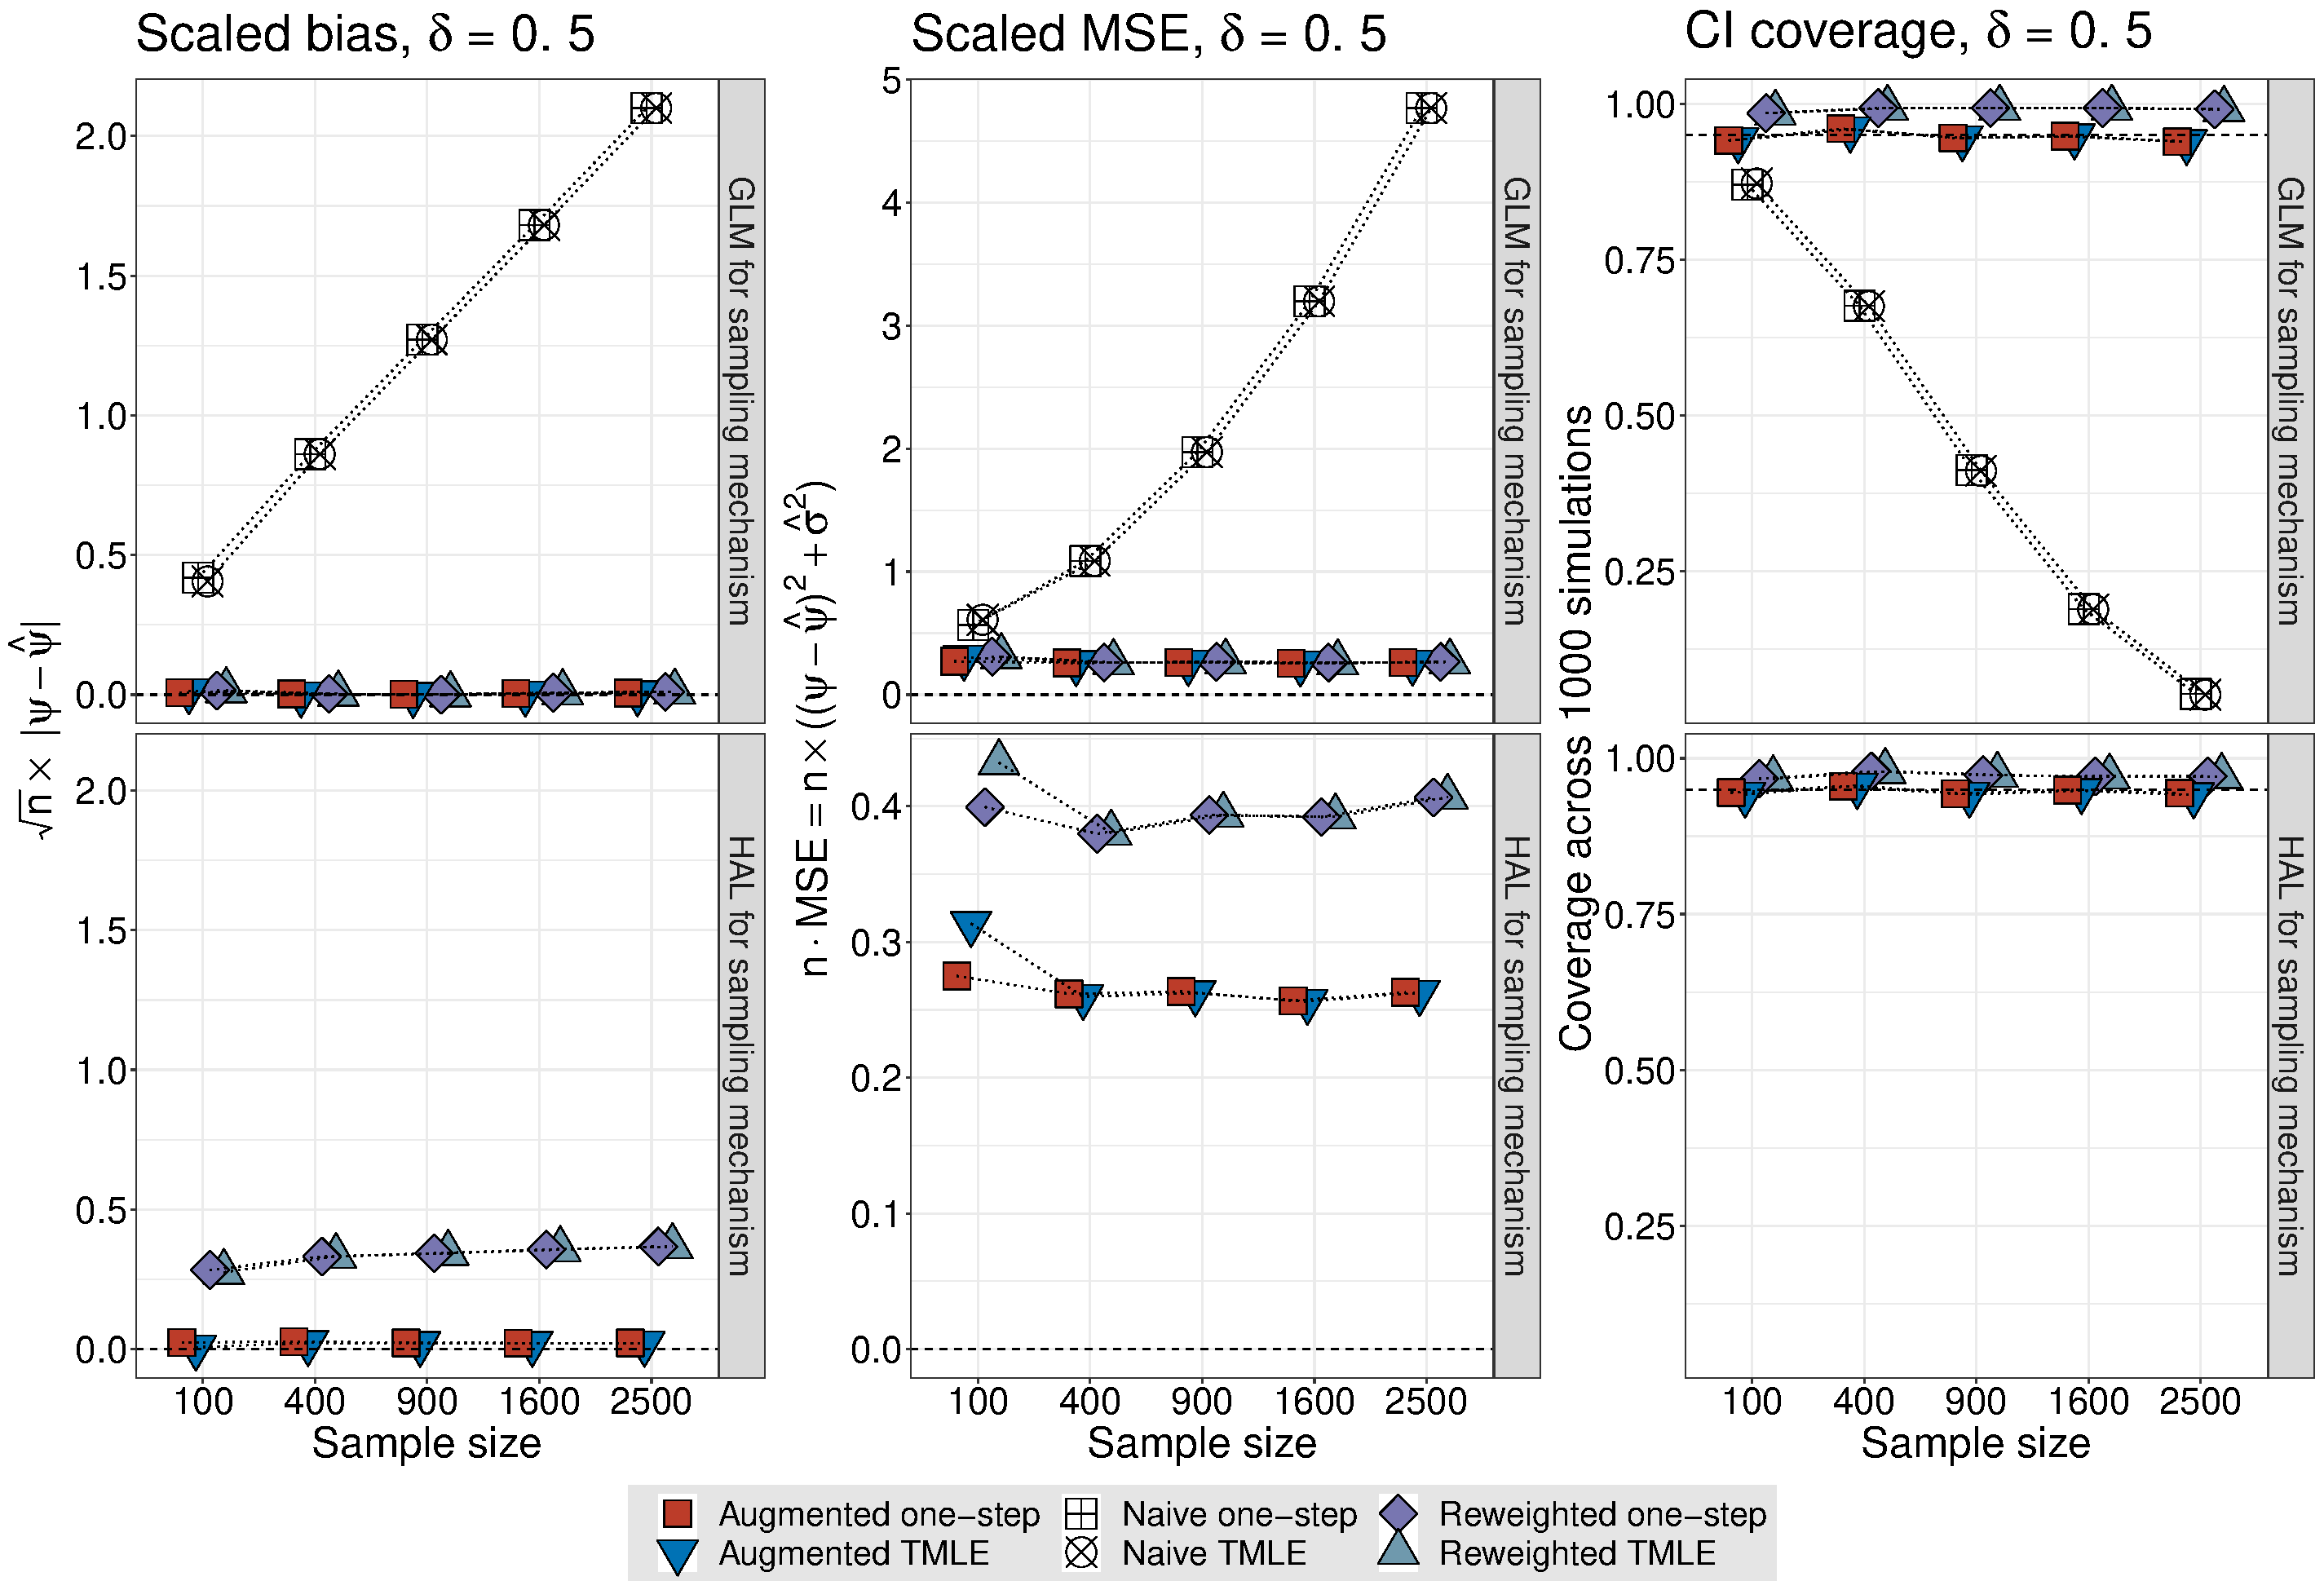
\includegraphics[scale=0.35]{simple_effect_panel_delta_upshift}
  \caption{Comparison of six estimation strategies
  for $\psi_{0,\delta}$ for $\delta = 0.5$, across 1000 Monte Carlo simulations
  for each of five sample sizes. The naive estimators do not make use of the
  estimated sampling mechanism $g_{n,C}$, so their performance is displayed
  only in the upper panel, in the interest of visual economy. This figure
  appears in color in the electronic version of this article, and any mention
  of color refers to that version.}
  \label{fig:simple_sim_delta_upshift}
\end{figure}

When the sampling mechanism is estimated via a correctly specified parametric
model (upper panel), the reweighted and our proposed estimators behave as
expected, with low bias and stable MSE. However, the reweighted estimators
display coverage exceeding 95\%, while our proposed estimators achieve nominal
coverage. This occurs because the influence function that is basis for the
standard error estimates does not include a first-order contribution resulting
from estimation of the sampling mechanism resulting in a conservative standard
error estimate. Unsurprisingly, the naive estimator performed poorly in all
sample sizes, highlighting the importance of accounting for sampling design.

When the sampling mechanism was estimated using HAL (lower panel), the
reweighted estimators do not attain asymptotic linearity, as evidenced by the
scaled bias and MSE increasing with sample size. On the other hand our proposed
estimators have small bias and MSE approaching the efficiency bound, thus
demonstrating the benefits of the additional effort required to produce our
estimators over the simpler reweighted estimators.

Our second simulation study (Section~\ref{sm}) showed that the
efficient estimators provide reliable performance in a setting similar to HVTN
505. Importantly, this setting incorporates both continuous and binary baseline
covariates and a rare outcome ($\approx$5\% incidence). We examine the
performance of our proposed one-step and TML estimators at a sample size of $n
= 1400$ across $\delta \in \{-2, -1.5, -1, 0.5, 0, 0.5, 1, 2\}$ and all nuisance
parameters were estimated via HAL. We found that the proposed estimators achieve
low bias and MSE, as well as empirical coverage of confidence intervals near the
nominal rate. Overall, the TML estimator had slightly better performance than
the one-step estimator.

\section{Application to the HVTN 505 Trial}\label{application}

HVTN 505 enrolled $2504$ HIV-negative participants and randomized participants
1-to-1 to receive an active vaccine or placebo. The one-year incidence of HIV-1
infection was about 1.8\% per person-year in the vaccine arm and 1.4\% per
person-year in the placebo arm, during primary follow-up for HIV-1 acquisition
(between week 28 and month 24; the same period as was used for assessment of
immune correlates). Blood was drawn at the week 26 visit and immune responses
measured for all HIV-1 cases diagnosed between week 28 and month 24 and
a stratified random sample of uninfected controls~\citep{janes2017higher}. The
two-phase sampling of vaccine-recipient controls sampled five controls per case
without-replacement within each of eight baseline covariate strata defined by
categories of body mass index and race/ethnicity (White, Hispanic, Black).
\citet{janes2017higher} and \citet{fong2018modification} analyzed these immune
responses, and both found CD4+ and CD8+ polyfunctionality scores to be
associated with risk of HIV-1 infection status by month 24.

We examined how a range of posited shifts in standardized polyfunctionality
scores of the CD4+ and CD8+ immune markers ($A$) would impact the mean
counterfactual risk of HIV-1 infection ($Y$) in vaccine recipients. We
considered \textit{standardized} polyfunctionality scores, so that our
pre-specified grid of shifts $\delta \in \{-2.0, -1.5, -1.0, -0.5, \allowbreak
0.0, 0.5, 1.0, 1.5, 2.0\}$ can be interpreted as shifts on the standard
deviation (sd) scale. We present results based on our TML estimator; results for
the one-step estimator were similar. To summarize the relationship between the
mean counterfactual risk of HIV-1 infection and shifts in polyfunctionality
scores, a working marginal structural model (MSM) was constructed, as detailed
in section~\ref{msm_summary} of Section~\ref{sm}. Our
augmented TML estimator $\psi_{n,\delta}^{\star}$ requires the construction of
initial estimators of all nuisance functions.

The conditional probability of inclusion in the second-phase sample was
estimated using HAL, adjusting for age, sex, race/ethnicity, body mass index,
and a behavioral risk score for HIV-1 infection. The density $q_{n,A}$ of the
CD4+ or CD8+ polyfunctionality scores ($A$), conditional on the same set of
covariates ($W$), was estimated using our proposed HAL-based conditional density
estimator. The outcome regression $\overline{Q}_{0,Y}$, which estimated the risk
of HIV-1 infection by 24 months ($Y$) given polyfunctionality score and baseline
covariates, was estimated using super learner~\citep{vdl2007super} (details in
Section~\ref{sm}). The pseudo-outcome regression, $G_n$, was
fit via HAL.

Results of applying our estimation procedure separately to both the CD4+ and
CD8+ polyfunctionality scores are presented in
Figure~\ref{fig:hvtn505_tmle_msm}.

\begin{figure}[H]
  \begin{subfigure}{0.9\textwidth}
  \centering
  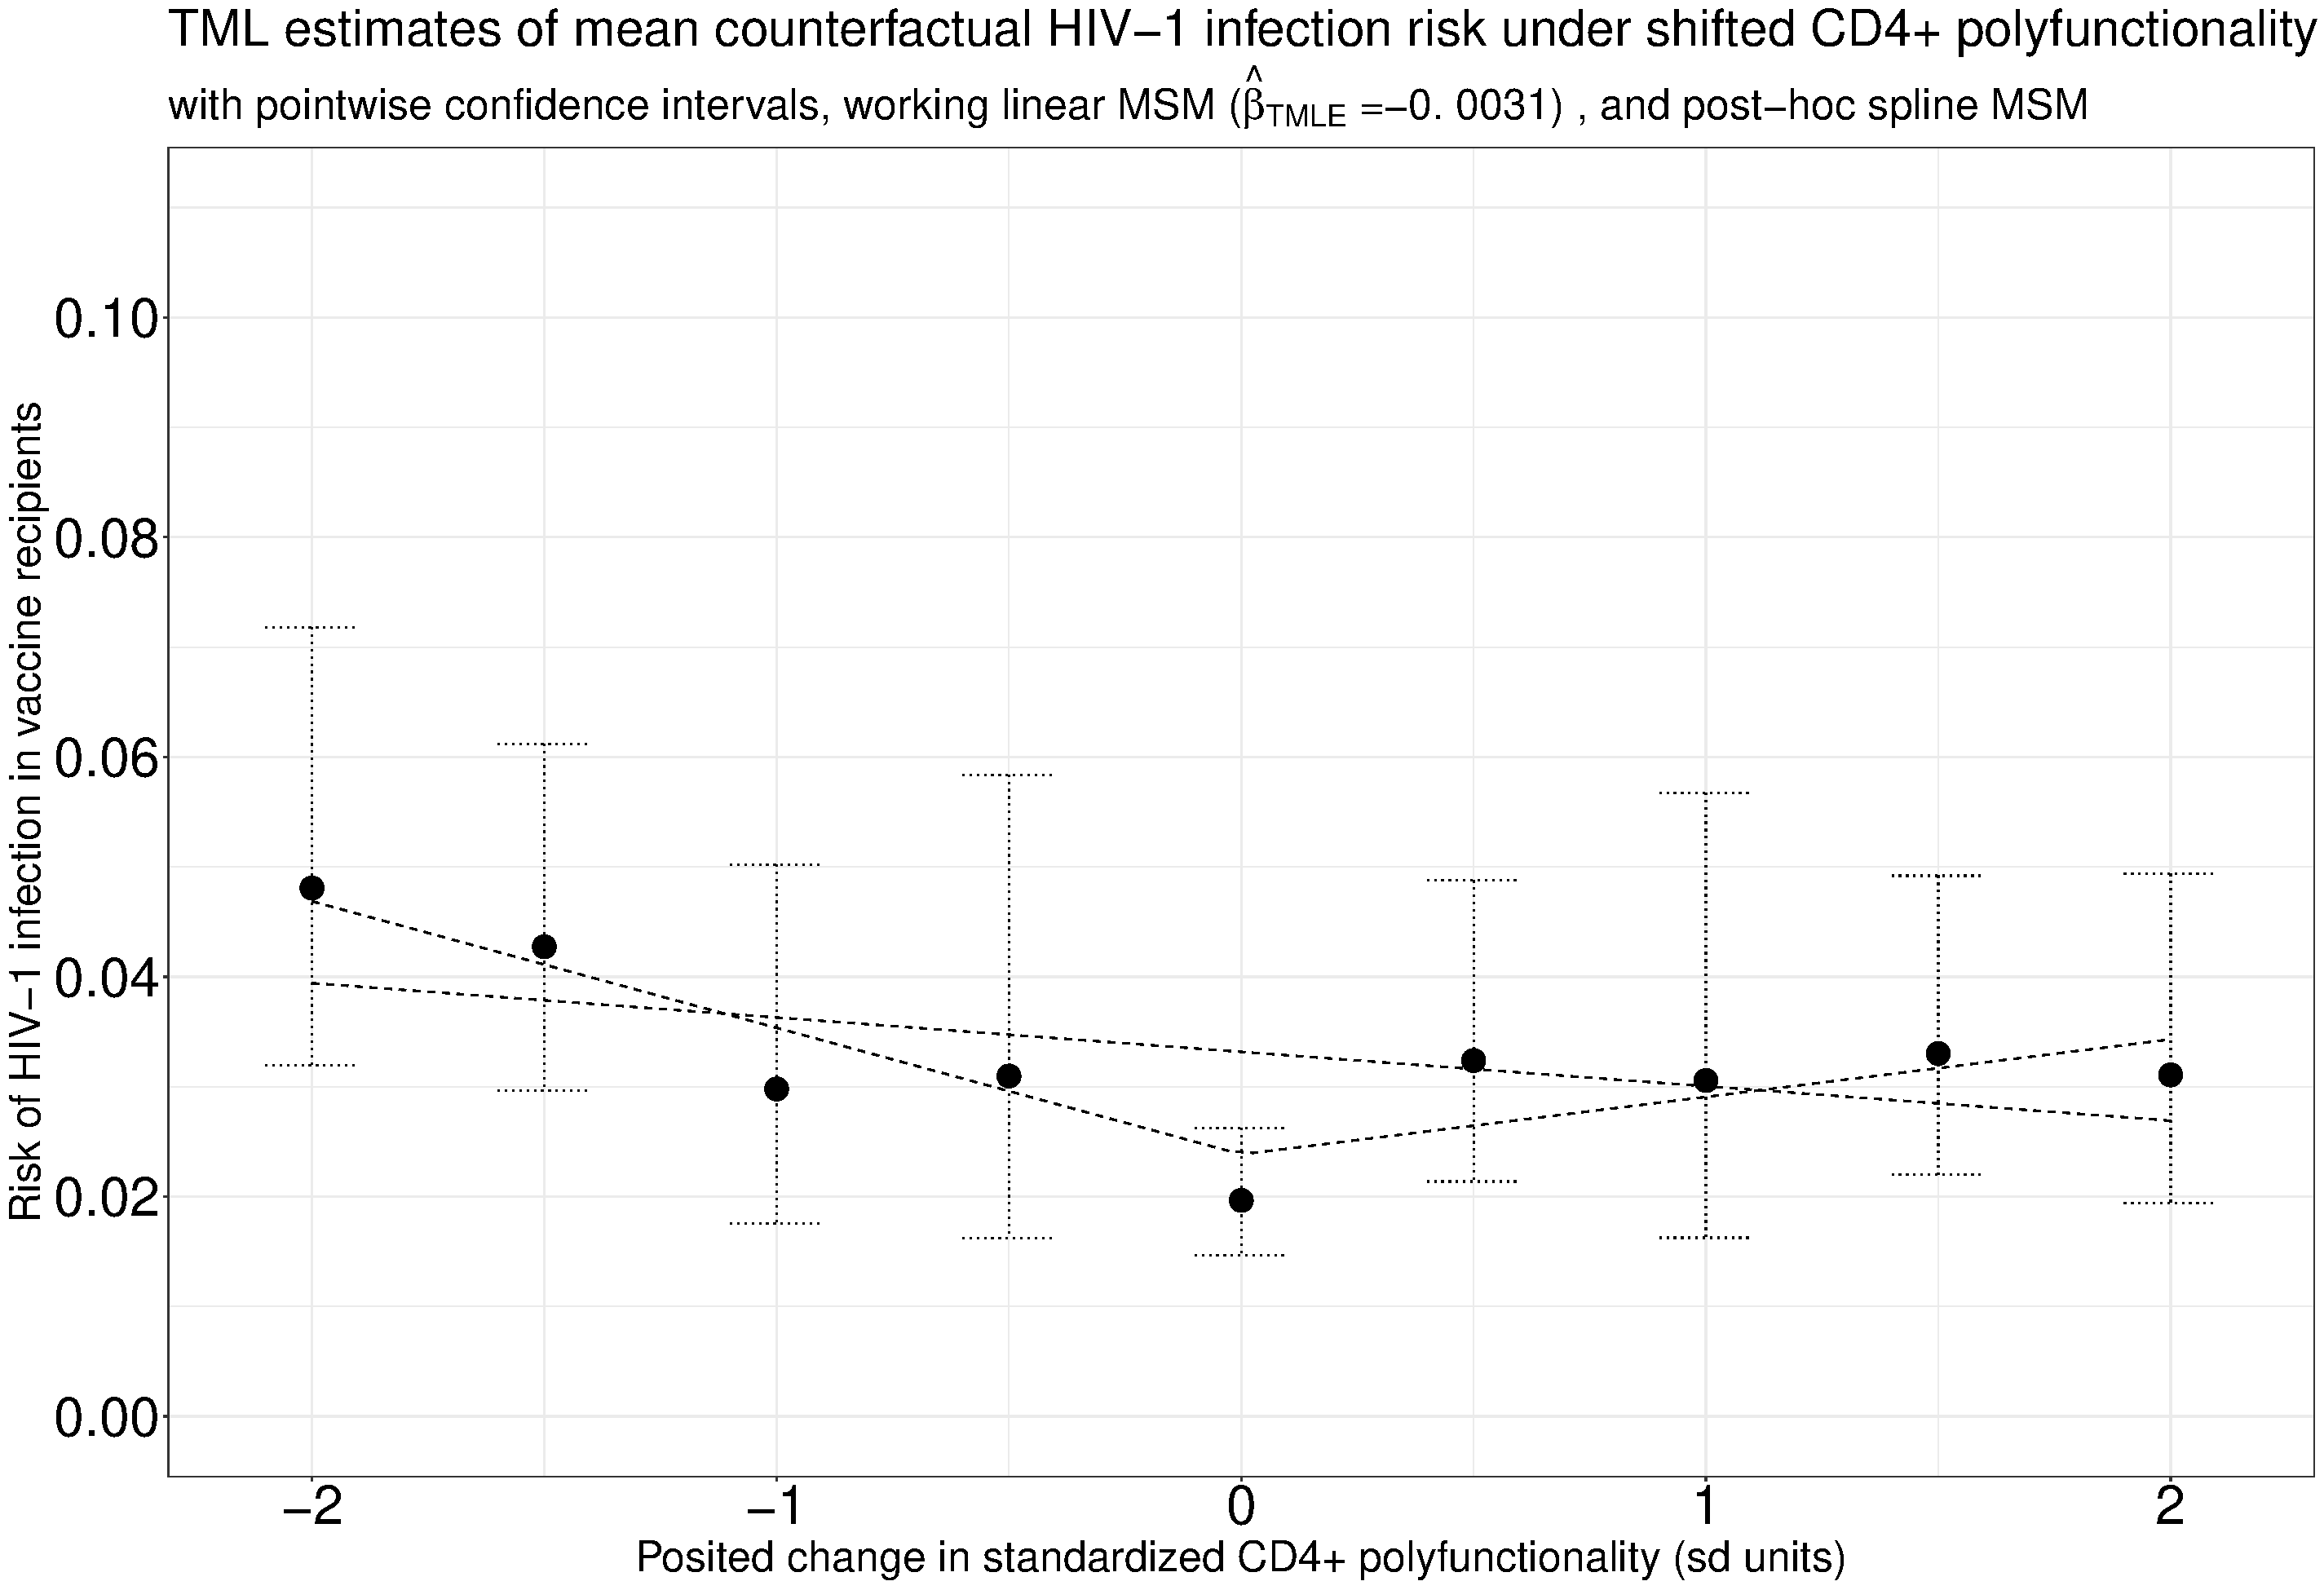
\includegraphics[scale=0.3]{cd4_msm_tmle_summary}
  \label{fig:cd4_tmle_msm}
  \end{subfigure}\\[0.5cm]
  \begin{subfigure}{0.9\textwidth}
  \centering
  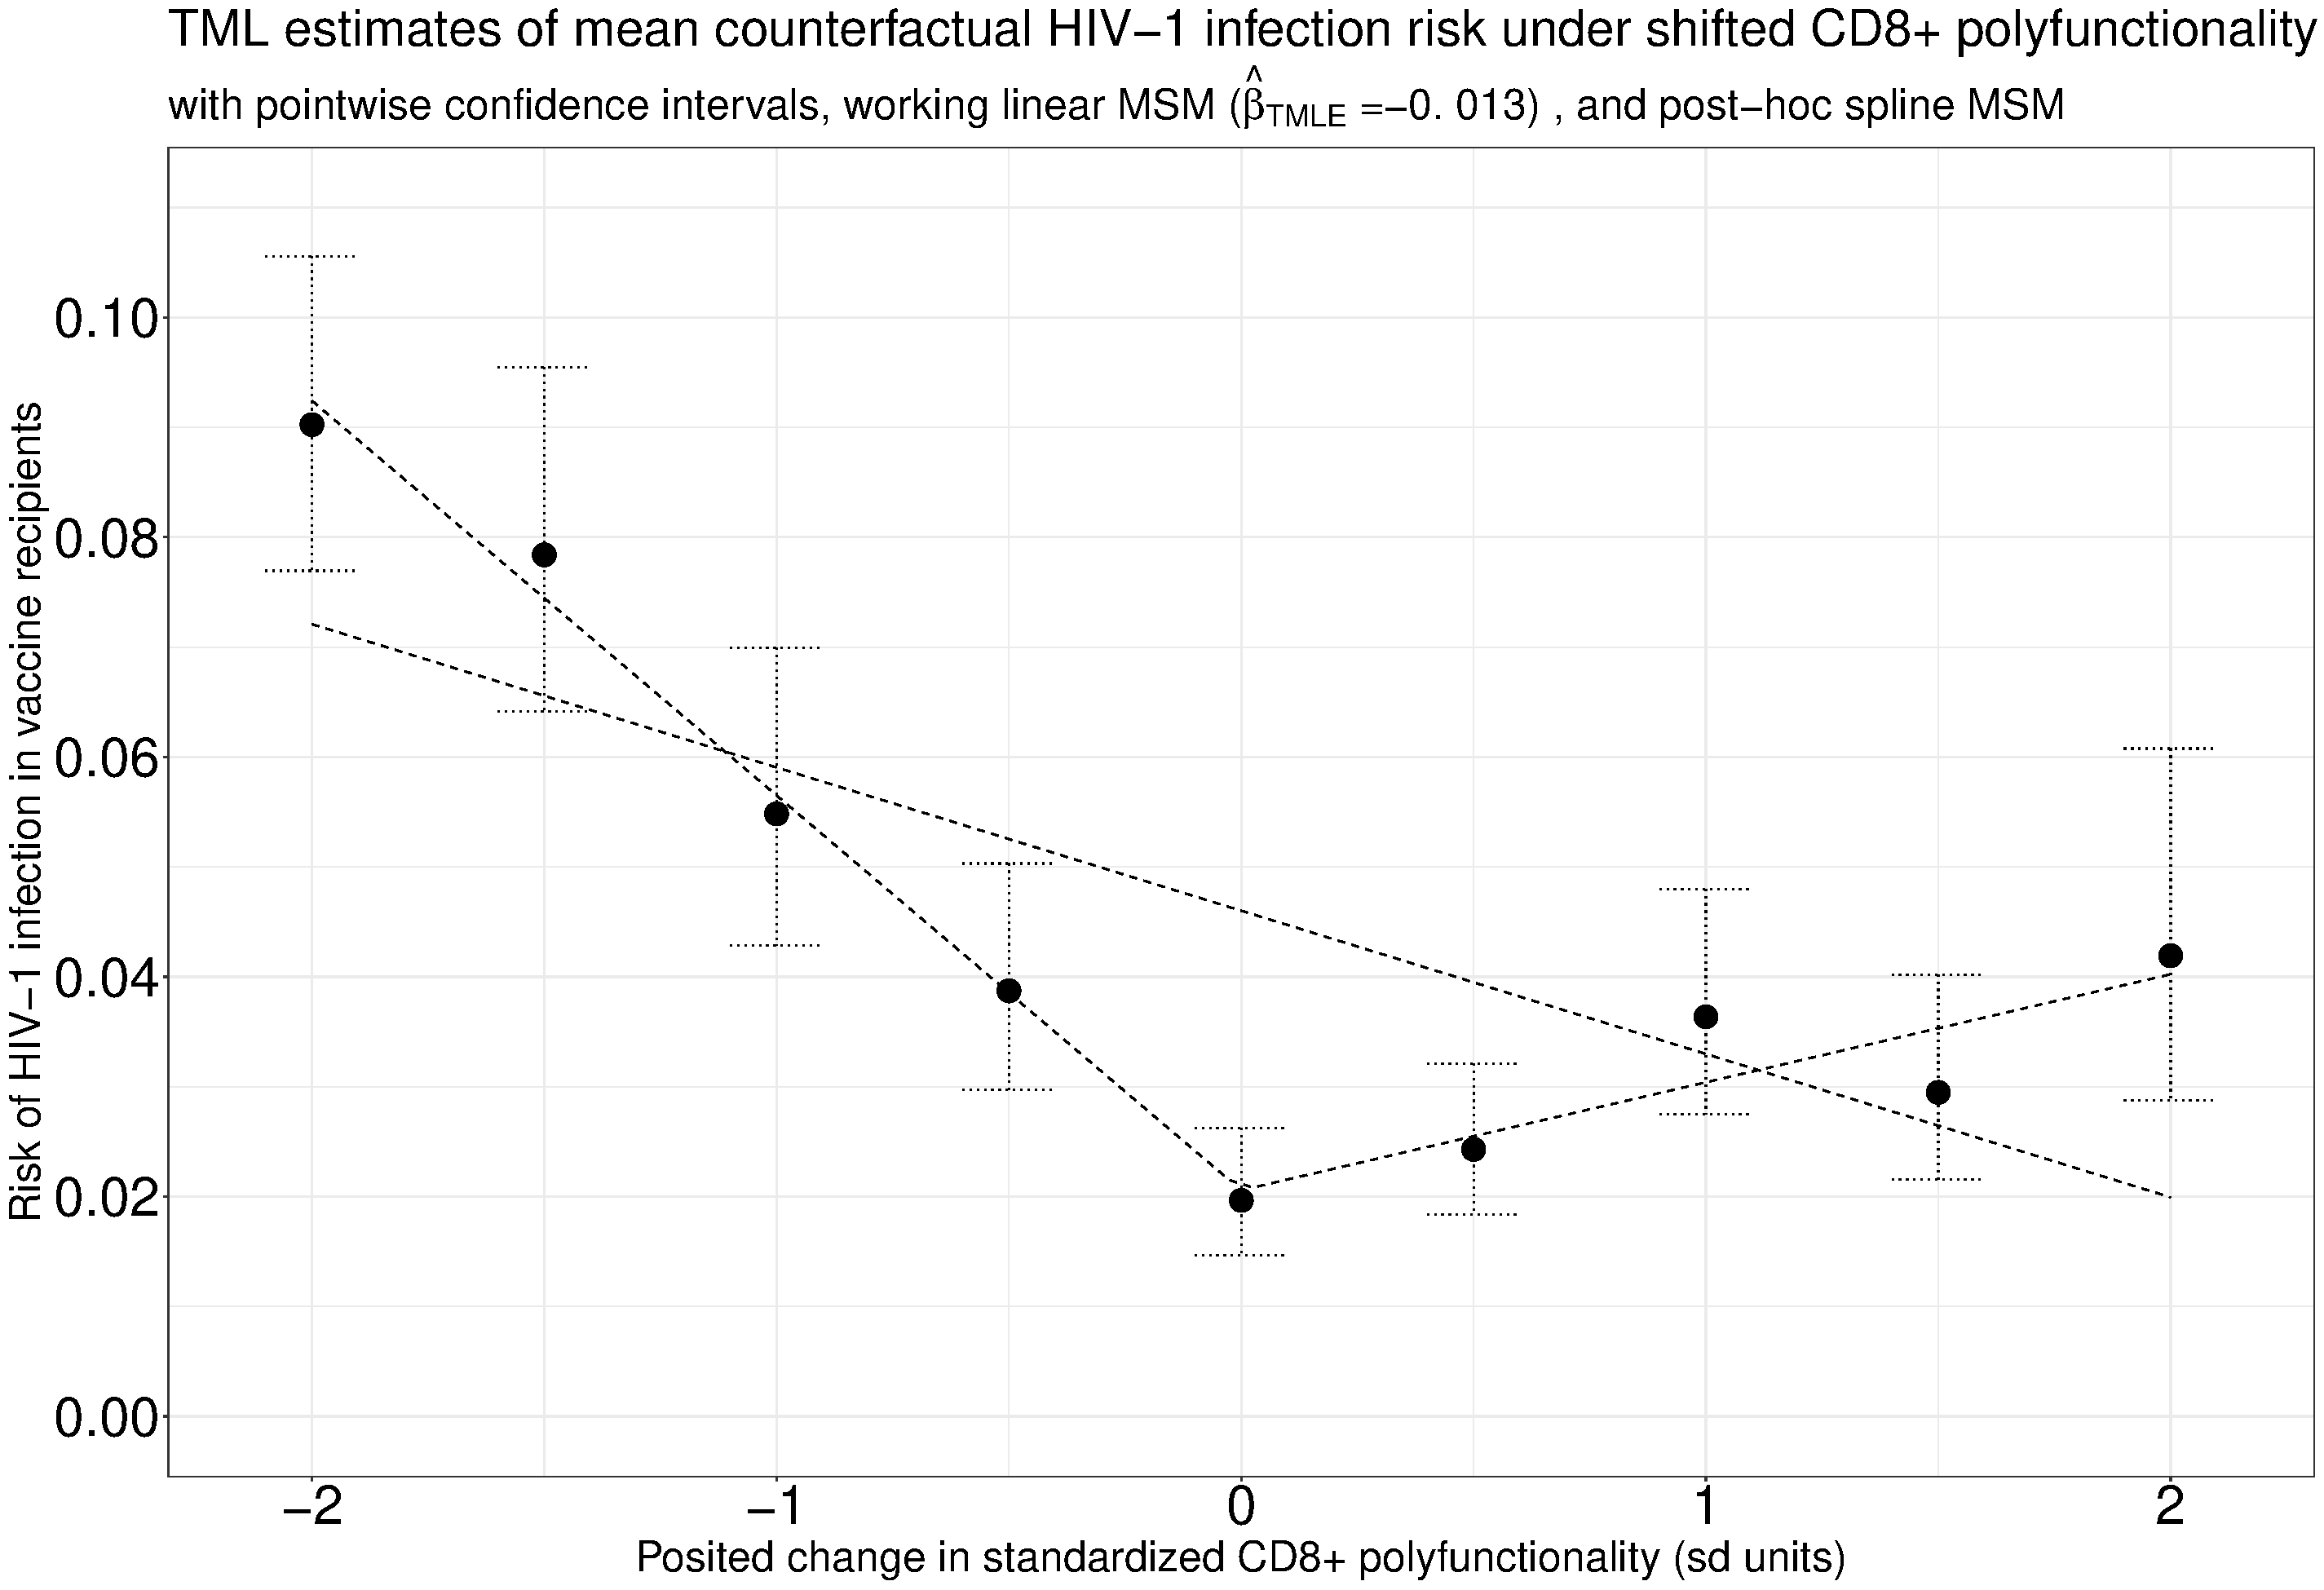
\includegraphics[origin=c,scale=0.3]{cd8_msm_tmle_summary}
  \label{fig:cd8_tmle_msm}
  \end{subfigure}
  \caption{TML estimates of the counterfactual mean of HIV-1 infection in
    vaccine recipients under stochastic interventions on CD4+ (top) and CD8+
    (bottom) standardized polyfunctionality scores. Inference for the estimates
    is based on pointwise Wald-type confidence intervals. The slope of a linear
    working MSM $\hat{\beta}_{\text{TMLE}}$, whose linear form is postulated
    \textit{a priori}, summarizes the effect of shifting the polyfunctionality
    scores on the mean counterfactual risk of HIV-1 infection. A spline model,
    whose V-shape appears to more closely trace the profile of counterfactual
    HIV-1 risk changes with $\delta$, was constructed post-hoc.}
  \label{fig:hvtn505_tmle_msm}
\end{figure}

Examination of the point estimates and confidence intervals of $\psi_{0,\delta}$
in Figure~\ref{fig:hvtn505_tmle_msm} reveals that downshifts in the CD4+
polyfunctionality score led to a small increase in estimated HIV-1 infection
risk among vaccine recipients (Figure~\ref{fig:hvtn505_tmle_msm}, top panel).
For example, examining the individual point estimates, a shift of two standard
units lower in the CD4+ polyfunctionality score was found to at least double the
counterfactual risk of HIV-1 infection. The estimated slope parameter of the
working MSM $\hat{\beta}_{\text{TMLE}}$ pointed to an estimated decrease in risk
of about -0.3\% per standard unit of CD4+ polyfunctionality change.

The estimated result of shifts in the polyfunctionality score of the CD8+
immunological marker displayed a markedly stronger relationship with the risk of
HIV-1 infection (Figure~\ref{fig:hvtn505_tmle_msm}, lower panel). Positive
shifts of the standardized CD8+ polyfunctionality score beyond those observed in
the trial do not appear to have a strong effect on HIV-1 infection risk;
confidence intervals for counterfactual risk estimates for all $\delta \geq 0$
overlap. On the other hand, shifts that lower the CD8+ polyfunctionality score
display a negative linear trend; moreover, confidence intervals for HIV-1 risk
estimates at all $\delta < 0$ do not overlap with those of the estimate at
$\delta = 0$. While this may be taken to indicate that decreases in CD8+ marker
activity adversely affect the risk of HIV-1 infection, we note that this
evidence should be weighed against the fact that all point estimates for
$\delta \neq 0$ are, in fact, higher than that at $\delta = 0$; thus, an
abundance of caution is warranted in drawing conclusions as to whether shifted
CD8+ polyfunctionality score would have improved the HVTN 505 vaccine. Still, it
may be informative that the counterfactual HIV-1 infection risk is over four
times that observed in the HVTN 505 trial at the largest negative shift
considered.
%that is, a vaccine inducing a significantly attenuated immune
%response would have been far less efficacious, underscoring the importance of
%post-vaccination immune response mechanisms in the infection process.

Overall, the results of our analyses support the conclusions of
\citet{janes2017higher} and \citet{fong2018modification}, further indicating
that modulation of the CD4+ and CD8+ polyfunctionality scores may reduce the
risk of HIV-1 infection, with CD8+ polyfunctionality playing a particularly
important role. Notably, our analysis differs from the previous efforts in two
ways: our estimates (i) are based on a formal causal model, which provides an
alternative estimand to summarize relationships between immunogenic response and
risk of HIV-1 infection, and (ii) leverage  machine learning to allow the use of
flexible modeling strategies while simultaneously delivering robust inference.

\section{Discussion}\label{discuss}

A possible criticism of our approach is that, in the context of vaccines, the
immune responses we consider may not be directly manipulable. Nevertheless, we
believe the estimands that we consider pass the important litmus test question:
``If we knew the value of the estimand, could we do something useful with it to
advance science?''~\citep{gilbert2011commentary}. Knowledge of which immune
responses may lead to the largest decrease in infection or disease incidence
would advance vaccine science and stimulate new ideas for the next generation of
vaccine research. Another challenge associated with our approach, as with many
examples in causal inference, is selecting a scientifically meaningful
intervention (i.e., modification of the exposure distribution). While we focused
here on additive shifts for simplicity, more scrutiny of this choice is
warranted in practice. Scientific context could provide some clues as to
potentially meaningful shifts. For example, in the context of influenza
vaccination, past studies have shown that repeated vaccinations may have
a dulling effect on immune responses to new
vaccines~\citep{thompson2016effects}. When such covariate data are available,
they could be used to define an appropriate shift, where the proposed shift is
lessened for individuals with many prior vaccinations.

Our analysis of the HVTN 505 trial could be improved in several respects. First,
there was participant dropout observed in the trial, which our analysis ignored.
A more robust analysis could leverage available covariate information to account
for potentially informative missingness. Further, while we investigate the
effect of altering post-vaccination immune responses on HIV-1 infection, the
issue of interference could limit identifiability of our target causal effects.
In trials conducted across geographically diverse sites or within short time
frames, it may be reasonable to assume that the potential protection conferred
by immune response in a given unit would not alter the infection process in
another unit, satisfying the lack of interference requirement for
identifiability of the causal parameter of interest. Indeed, there is a growing
body of work on relaxing this condition in causal
inference~\citep[e.g.,][]{hudgens2008toward}.

Beyond this issue, there are several other directions for potentially
interesting extensions. First, when a range of shifts is of interest as in our
example, we summarized linear trends using working marginal structural models.
An alternative formulation could examine the stronger null hypothesis that $H_0:
\E Y_{\delta} = \E Y$, uniformly in $\delta$. This is analogous to the
hypothesis tests of~\citet{kennedy2019nonparametric}, which deals with shifted
binary exposure distributions. There, the authors propose a test of this strong
null hypothesis and describe methods for obtaining simultaneous confidence bands
using the multiplier bootstrap. Second, it is of interest to extend our
estimation strategy to other effects based on stochastic interventions, such as
the population intervention (in)direct effects~\citep{diaz2020causal}. Extending
our estimation strategy to such settings and its application in analyzing other
vaccine efficacy trials will be the subject of future research.

\section{Supplementary Materials}\label{sm}

While no new data were generated or analyzed in the present work, the results of
our reported analyses may be reproduced using the publicly available \texttt{R}
code at \url{https://github.com/nhejazi/pub_txshift_biometrics}. Throughout our
simulation experiments and data analyses, we rely on our \texttt{txshift} and
\texttt{haldensify} \texttt{R} packages, available at
\url{https://github.com/nhejazi/txshift} and
\url{https://CRAN.R-project.org/package=haldensify}, respectively. The
\texttt{txshift} \texttt{R} package implements our proposed efficient estimators
of the counterfactual mean outcome under a stochastic intervention, while our
\texttt{haldensify} \texttt{R} package provides a nonparametric estimator of the
generalized propensity score.

\subsection{Conditional density estimation based on the highly adaptive
lasso}\label{cond_dens}

In section~\ref{est_nuisance_param}, several of the challenges associated
with conditional density estimation were briefly expressed. The auxiliary
covariate appearing in the form of the EIF is a ratio of such conditional
densities. In the construction of our proposed estimators, the exposure
mechanism $q_{0,A}$ is a density of the intervention $A$, conditional on the
observed covariates $W$, which must be evaluated at both the observed values and
the post-intervention counterfactual values. As consistent estimation of the the
generalized propensity score is an integral part of our proposed methodology, we
outline here a conditional density estimator, built around the HAL regression
function, that achieves the convergence rate required by our formal theorem. We
note that proposals for the data adaptive estimation of such quantities are
sparse in the literature~\citep[e.g.,][]{zhu2015boosting}. Notably,
\citet{diaz2011super} gave a proposal for constructing semiparametric estimators
of such a target quantity based on exploiting the relationship between the
hazard and density functions. Our proposal builds upon theirs in several key
ways: (i) we adjust their algorithm so as to incorporate sample-level weights,
necessary for making use of inverse probability of censoring weights; and (ii)
we replace their use of an arbitrary classification model with one based on the
HAL regression function. While our first modification is general and may be
applied to the estimation strategy \citet{diaz2011super} propose, our latter
contribution requires adjusting the penalization aspect of HAL regression to
respect the use of a loss function appropriate for prediction on the hazard
scale. To make these contributions widely accessible, we introduce the
\texttt{haldensify} \texttt{R} package~\citep{hejazi2020haldensify}, available
at \url{https://github.com/nhejazi/haldensify}

To build an estimator of a conditional density, \citet{diaz2011super} considered
discretizing the observed $a \in A$ based on a number of bins $T$ and a binning
procedure (e.g., including the same number of points in each bin or forcing
bins to be of the same length). We note that the choice of the tuning parameter
$T$ corresponds roughly to the choice of bandwidth in classical kernel density
estimation; this will be made clear upon further examination of the proposed
algorithm. The data $\{A, W\}$ are reformatted such that the hazard of an
observed value $a \in A$ falling in a given bin may be evaluated via standard
classification techniques. In fact, this proposal may be viewed as
a re-formulation of the classification problem into a corresponding set of
hazard regressions:
$\prob (a \in [\alpha_{t-1}, \alpha_t) \mid W) = \prob (a \in [\alpha_{t-1},
\alpha_t) \mid A \geq \alpha_{t-1}, W) \times \prod_{j = 1}^{t -1} \{1 - \prob
(a \in [\alpha_{j-1}, \alpha_j) \mid A \geq \alpha_{j-1}, W) \}$,
where the probability that a value of $a \in A$ falls in a bin $[\alpha_{t-1},
\alpha_t)$ may be directly estimated from a standard classification model. The
likelihood of this model may be re-expressed in terms of the likelihood of
a binary variable in a data set expressed through a repeated measures structure.
Specifically, this re-formatting procedure is carried out by creating a data set
in which any given observation $A_i$ appears (repeatedly) for as many intervals
$[\alpha_{t-1}, \alpha_t)$ that there are prior to the interval to which the
observed $a$ belongs. A new binary outcome variable, indicating $A_i \in
[\alpha_{t-1}, \alpha_t)$, is recorded as part of this new data structure. With
the re-formatted data, a pooled hazard regression, spanning the support of $A$
is then executed. Finally, the conditional density estimator
$q_{n, \alpha}(a \mid W) = (\prob(a \in [\alpha_{t-1}, \alpha_t) \mid W)) /
(\alpha_t - \alpha_{t-1})$,
for $\alpha_{t-1} \leq a < \alpha_t$, may be constructed. As part of this
procedure, the hazard estimates are mapped to density estimates through
rescaling of the estimates by the bin size ($\alpha_t - \alpha_{t-1}$).

In its original proposal, a key element of this procedure was the use of any
arbitrary classification procedure for estimating $\prob(a \in [\alpha_{t-1},
\alpha_t) \mid W)$, facilitating the incorporation of flexible, data adaptive
estimators. We alter this proposal in two ways, (i) replacing the arbitrary
estimator of $\prob(a \in [\alpha_{t-1}, \alpha_t) \mid W)$ with HAL regression
and (ii) accommodating the use of sample-level weights, making it possible for
the resultant conditional density estimator to achieve a convergence rate with
respect to a loss-based dissimilarity of $n^{-1/4}$ under only mild assumptions.
This is an important advance that is needed for the asymptotic analysis of our
proposed estimators, as per section~\ref{asymp_analy}. As a secondary
advance, our procedure alters the HAL regression function to use a loss function
tailored for estimation of the hazard, invoking $\ell_1$-penalization in
a manner consistent with this loss.

\subsection{Algorithm for efficient targeted minimum loss
  estimation}\label{tmle_algo}

In section~\ref{os_tml_est}, we introduced a novel algorithm for targeted
minimum loss estimation with inverse probability of censoring weights. We
formalize our procedure in Algorithm~\ref{alg:ipcw_targeting}:
\begin{algorithm}[H]
\label{alg:ipcw_targeting}
\SetAlgoLined
\KwResult{Updated sampling mechanism estimate $g_{n,C}^{\star}$ and updated
  outcome mechanism estimate $\overline{Q}_{n,Y}^{\star}$}
\SetKwInOut{Input}{Input}\SetKwInOut{Output}{Output}
\Input{
  \begin{itemize}
    \item[] Initial estimate of the sampling mechanism: $g_{n,C} \in [0, 1]$
    \item[] Initial estimate of the outcome mechanism: $\overline{Q}_{n,Y}
        \in \R$
    \item[] Estimate of the EIF pseudo-outcome regression: $G_n \in \R$
    \item[] Estimate of the auxiliary covariate of the EIF: $H_n \in \R$
    \item[] Observed indicators of the sampling mechanism: $C \in \{0, 1\}$
  \end{itemize}
}
\BlankLine
Initialize $g_{n,C}^{\star} \coloneqq 0$ and
$\overline{Q}_{n,Y}^{\star} \coloneqq 0$\;
\BlankLine
\While{$g_{n,C}^{\star} = 0$ and $\overline{Q}_{n,Y}^{\star} = 0$}{
Define a working logistic regression model $\logit(g_{n, C, \xi}) =
     \logit(g_{n,C}) + \xi (G_n / g_{n,C}) : \xi \in \R$ and evaluate the MLE
     $\xi_n$ of the parameter $\xi$, e.g., via iteratively reweighted least
     squares\;
With the MLE $\xi_n$, extract predictions from this working model for
    the outcome, the conditional mean of $C$ given $\{Y, W\}$, constructing the
    updated estimate $g_{n,C}^{\star} \coloneqq g_{n, C, \xi_n}$\;
Define a weighted working logistic regression model
    $\logit(\overline{Q}_{n, Y, \epsilon}) = \logit(\overline{Q}_{n,Y}) +
    \epsilon H_n : \epsilon \in \mathbb{R}$, with weights $C_i
    / g^{\star}_{n,C}(Y_i,W_i)$, and construct the MLE
    $\epsilon_n$ of the model parameter $\epsilon$\;
With the MLE $\epsilon_n$, construct the updated estimate of the
    outcome, the conditional mean of $Y$ given $\{A,W\}$, by prediction to
    obtain $\overline{Q}_{n,Y}^{\star} \coloneqq \overline{Q}_{n, Y,
    \epsilon_n}$.
}
\BlankLine
\Output{
  \begin{itemize}
    \item[] $g_{n,C}^{\star}$, an updated estimate of the sampling mechanism.
     \item[] $\overline{Q}_{n,Y}^{\star}$, an updated estimate of the outcome
       mechanism.
  \end{itemize}
}
\caption{Efficient updating procedure for IPCW-TML estimation}
\end{algorithm}
Note that in the two working logistic regression models defined above, the
inputs $g_{n,C}$ and $\overline{Q}_{n,Y}$ are both treated as offsets (known
parameter value equal to one); thus, the working models are one-dimensional.

The outlined procedure includes two targeting steps. The first of these steps
constructs an update of the initial estimator of the second-phase sampling
probability, $g_{n,C}^{\star}$, based on the initial estimate of $G_n$. This
step ensures that the revised estimate satisfies $\sum_{i=1}^n \{G_n(Y_i, W_i)
/ g_{n,C}^{\star}(Y_i,W_i\} \{C_i - g_{n,C}^{\star}(Y_i, W_i)\} = 0$. in
a single step when a universal least favorable submodel~\citep{vdl2016one} is
used, though an iterative procedure based on locally least favorable parametric
submodels may be used to achieve the same result. In the second step, the
updated outcome regression $\overline{Q}_{n,Y}^{\star}$ is generated based on
the conditional density estimate $q_{n,A}$; the inclusion of weights in the
regression ensures that $\sum_{i=1}^n C_i/g_{n,C}(Y_i, W_i) D_{n,i}^F = 0$.

\subsection{Summarization via working marginal structural
models}\label{msm_summary}

%\db{Basically, the point is that $\psi_{0,d}$ is like one
%counterfactual mean. So I can know the mean if I give everyone treatment, but
%that's only useful if I also know the mean when every one takes control. So we
%need to make explicit that we're trying to define an interesting
%\textit{contrast}.}
Estimation of $\psi_{0,\delta}$ for a single pre-specified shift $\delta$ may be
unsatisfactory in some contexts, as it does not provide information concerning
a dose-response relationship between exposure and outcome. Thus, to develop an
understanding of a dose-response pattern in the context of stochastic
interventions, it may be informative to estimate the counterfactual mean outcome
across several values of $\delta$. In the context of HVTN 505, we consider
estimation of a grid of counterfactual means $\psi_0 = (\psi_{n,\delta_1},
\ldots, \psi_{n,\delta_K})$ and examine how the risk of HIV infection varies
with choice of $\delta$ over a fixed grid, i.e., $\delta_k \in \{\delta_1,
\ldots, \delta_K\}$. After estimating the counterfactual mean for each
$\delta_k$, a summary measure relating the stochastic
interventions to the mean counterfactual outcomes may be constructed by
projection onto a working marginal structural model (MSM). For example, we might
consider a (possibly weighted) least-squares projection on the linear working
model $m_{\beta}(\delta) = \beta_0 + \beta_1 \delta$, in which case the
parameter $\beta_1$ corresponds to the linear trend in mean counterfactual
outcomes as a function of the $\delta_k$.

More generally, we can define $\beta(\delta)=\argmin_{\beta \in \mathbb{R}^d}
\sum_{\delta \in \{\delta_1, \ldots, \delta_K\}} h(\delta)\{\psi_{0,\delta}
- m_{\beta}(\delta)\}^2$, for a user-selected weight function $h(\delta)$. We
note that adjustment of the weight function, as well as the functional form of
$m_{\beta}(\delta)$, allow for a wide variety of working models to be
considered. Alternatively, $\beta(\delta)$ can be viewed as the solution of
\begin{equation*}
  0 = U(\beta,\psi) = \sum_{\delta \in \{\delta_1, \ldots, \delta_K\}}
  h(\delta) \frac{d}{d\beta} m_{\beta}(\delta) \{\psi_{0,\delta} -
  m_{\beta}(\delta)\}.
\end{equation*}
The goal is to make statistical inference on the parameter $\beta$. We note that
this approach does not assume a linear dose-response curve, but rather uses
a working model to summarize the relationship between exposure and outcome
\citep{neugebauer2007nonparametric}. This approach is distinct from that of
\citet{haneuse2013estimation}, whose proposal involving MSMs pertains
specifically to parametric models.

To estimate $\beta$, we assume access to the TML or one-step estimates $\psi_n
= (\psi_{n, \delta_1}, \ldots, \psi_{n,\delta_K})$ for each $\delta_k$. The
estimate $\beta_n$ of $\beta$ is the solution in $\beta$ of the equation $0
= U(\beta,\psi_n)$. To derive the limit distribution of $\beta_n$, let
$D_{0,\psi}$ denote a vector whose $k^{\text{th}}$ entry is the EIF associated
with parameter $\psi_{0,\delta_k}$. The delta method implies that the influence
function of $\beta_n$ is $D_{\beta} = [-\frac{d}{d \beta} U(\beta,\psi_0)^{-1}]
\frac{d}{d\psi_0} U(\beta, \psi_0) D_{\psi_0}$, and that $n^{1/2} (\beta_n
- \beta)$ converges in distribution to a mean-zero Gaussian random variable with
variance $\Sigma = \E_{P_0}\{D_{\beta}(O)^2\}$. The empirical covariance matrix
of $D_{0,\psi}$ evaluated at nuisance parameter estimates serves to estimate
$\Sigma$.

%\vdl{define $\beta(\delta)=\argmin_{\beta} \sum_{\delta}
%h(\delta)(\psi(\delta) - m_{\beta}(\delta))^2$ that solves
%$0=U(\beta,\psi) = \sum_{\delta} h(\delta) \frac{d}{d\beta} m(\psi(\delta) -
%m_{\beta}(\delta))$. This equation defines $\beta=\beta(\psi)$ as function of
%$\psi$-vector. The implicit function theorem says $\frac{d}{d \psi} \beta(\psi)
%= [-\frac{d}{d \beta} U(\beta, \psi)^{-1}] \frac{d}{d \psi} U(\beta,\psi)$ so
%$D_{\beta}=[-\frac{d}{d \beta} U(\beta,\psi)^{-1}] \frac{d}{d \psi}
%U(\beta,\psi) D_{\psi}$ (the last one is gradient on its side), where
%$D_{\psi}$ is vector efficient influence function of $\psi$ vector. the front
%is your matrix inverse. the last part if the gradient applied to $D_{\psi}$.}

%$\sum_{k = 1}^K h(\delta_k) \left(\psi_{0,\delta_k} -
%m_{\beta}(\delta_k) \right) \frac{d}{d\beta} m_{\beta}(\delta_k) = 0$, where
%$h(\delta)$ is a weight function. To estimate $\beta$ and derive confidence
%intervals and hypothesis tests for $\beta$, we note its EIF $D_{\beta}(O)$ may
%be written in terms of the EIFs $D_{\psi_{0,\delta_k}}(O)$ of the
%$\psi_{0,\delta_k}$ by application of the delta method, yielding
%\begin{equation*}
  %D_{\beta}(O) = \left(\sum_{k=1}^K h(\delta_k) \frac{d}{d\beta}
  %m_{\beta}(\delta_k) \frac{d}{d\beta} m_{\beta}(\delta_k)^T \right)^{-1} \cdot
  %\sum_{k=1}^K h(\delta_k) \frac{d}{d\beta} m_{\beta}(\delta_k)
  %D_{\psi_{0,\delta_k}}(O).
%\end{equation*}
%Substituting the linear working MSM for an analogous generalized linear model
%allows this projection approach to be applied to arbitrary finite-dimensional
%regression models.

%\db{I couldn't really follow this math. What is $h$? I would just show the math
%explicitly for the linear regression example (i.e., show how to compute
%estimators, get standard error estimates, build confidence intervals), and just
%state that the ideas generalize the projections onto arbitrary
%finite-dimensional regression models.}
%we note the first-order
%expansion $\beta(\widetilde{\psi}_{n,d}) - \beta(\widetilde{\psi}_{0,d}) \approx
%- \frac{d}{d\beta} u(\beta_0, \widetilde{\psi}_{0,d})^{-1} \frac{d}{d\psi}
%u(\beta_0, \psi_0)(\widetilde{\psi}_{n,d} - \widetilde{\psi}_{0,d})$, where
%where we have
%$\frac{d}{d\beta} u(\beta, \psi) = -\sum_{\delta} h(\delta) \frac{d}{d\beta}
%m_{\beta}(\delta)^t \frac{d}{d\beta} m_{\beta}(\delta),$
%and $\frac{d}{d\psi}u(\beta, \psi)(\psi_n - \psi_0) = \sum_{\delta} h(\delta)
%\frac{d}{d\beta} m_{\beta}(\delta) (\psi_n - \psi_0)(\delta)$.

\subsection{Proof of Theorem~\ref{theo:aslintmle}}

We now examine a proof of the theorem establishing conditions for the weak
convergence of our efficient estimators. Building upon
section~\ref{background}, note that the full data parameter may be
expressed as a mapping $\Psi^F: \M^X \rightarrow \R$ and that $\Psi^F(P_0^X)
\equiv \Psi^F(\overline{Q}_{0,Y})$, since the parameter mapping depends on
$P_0^X$ only through the functional $\overline{Q}_{0,Y}$. We recall that the EIF
$D^F(\overline{Q}_{0,Y},g_{0,A})$ coincides with the canonical gradient of the
parameter mapping $\Psi^F: \M^X \rightarrow \R$, since a regular asymptotically
linear estimator with influence function equal to the canonical gradient is
asymptotically efficient~\citep{bickel1993efficient, vdl2003unified}. Note
further that the observed data parameter is defined such that $\Psi(P_0) \equiv
\Psi^F(P^X_0)$, where the observed data parameter mapping $\Psi:\M \rightarrow
\R$ is pathwise differentiable at a distribution $P$ in the statistical model
with a gradient given by the EIF:
\begin{equation*}
  D(G_0, g_{0,C}, D^{F}(\overline{Q}_{0,Y}, q_{0,A}))(o) =
  \frac{C}{g_{0,C}(y, w)} D^F(\overline{Q}_{0,Y}, q_{0,A})(x) -
  \frac{G_0(y,w)}{g_{0,C}(y,w)}(C - g_{0,C}(y,w)) \ .
\end{equation*}
The class of all gradients of $\Psi$ at $P$ is given by $\{D(G_0, g_{0,C},
D^F(P^X)): D^F(P^X)\}$ where $D^F(P^X)$ varies over all gradients of the
full data parameter $\Psi^F$ at distributions $P^X \in \M^X$. As $D^F$ varies,
$G_0$ also necessarily varies since it is defined as the conditional mean of
$D^F$ given $\{C = 1, Y, W\}$. In particular, if the full data model $\M^X$ is
nonparametric, then there is only one full data gradient, which is the canonical
gradient (or EIF) of $\Psi$ at $P$.

In the sequel, let $\lVert f \rVert_2 = \E\{f(O)^2\}^{1/2}$ denote the
$L^2(P_0)$ norm of a $P_0$-measurable function $f$, define $\widetilde{G}_0
\coloneqq \E_{P_0}[D^F(\overline{Q}^{\star}_{n,Y}, q_{n,A})(O) \mid C = 1, Y,
W]$, and let $G_n$ be the estimate of $\widetilde{G}_0$. An exact
characterization of the second-order remainder for the full data parameter
$\Psi^F(P^X) - \Psi^F(P_0^X)$ is given by
\begin{equation*}
  R^F_2(\overline{Q}_{n,Y}, q_{n,A}, \overline{Q}_{0,Y}, q_{0,A}) \coloneqq
    \Psi^F(\overline{Q}_{n,Y})-\Psi^F(\overline{Q}_{0,Y}) +
    \E_{P^X_0}[D^F(\overline{Q}_{n,Y}, q_{n,A})]
\end{equation*}
while the exact second-order remainder for the observed data parameter
$\Psi(P)-\Psi(P_0)$ is analogously defined
\begin{equation*}
  R_2(P, P_0) \coloneqq \Psi(P) - \Psi(P_0) + \E_{P_0}[D(G_n, g_{n,C},
  D^F(\overline{Q}_{n,Y}, q_{n,A}))].
\end{equation*}
Combining these definitions, the exact second-order remainder for the observed
data parameter may be expressed in terms of the second-order remainder of its
full data counterpart:
\begin{equation*}
  R_2(P, P_0) = R_2^F(\overline{Q}_{n,Y}, q_{n,A}, \overline{Q}_{0,Y}, q_{0,A})
    + \E_{P_0} \left[ \left(\frac{g_{n,C} - g_{0,C}}{g_{n,C}} \right) (G_n -
    \widetilde{G}_0) \right].
\end{equation*}

Assume the following conditions:
\begin{assumption}\label{ass:eif_rootn}
  $\E_{P_n} D(G_n, g^{\star}_{n,C}, D^F(\overline{Q}^{\star}_{n,Y},
    q_{n,A})) = 0$.
\end{assumption}
\begin{assumption}\label{ass:sampling_bound}
  $g_{0,C} > \zeta > 0$ and $g^{\star}_{n,C} > \zeta$ with probability tending
  to 1 for some $\zeta > 0$.
\end{assumption}
\begin{assumption}\label{ass:obs_eif_parametric}
    $\lVert G_n - \widetilde{G}_0 \rVert_{P_0} = o_P(n^{-1/4})$ and
        $\lVert g^{\star}_{n,C} - g_{0,C} \rVert_{P_0} = o_P(n^{-1/4})$.
\end{assumption}
\begin{assumption}\label{ass:r2_fulldata}
  $R_2^F(\overline{Q}^{\star}_{n,Y}, q_{n,A}, \overline{Q}_{0,Y},
       q_{0,A}) = o_P(n^{-1/2})$.
\end{assumption}
\begin{assumption}\label{ass:neglig_obs_eif}
   $\lVert D(G_n, g^{\star}_{n,C}, D^F(\overline{Q}^{\star}_{n,Y},
        q_{n,A})) - D(G_0, g_{0,C}, D^{F}(\overline{Q}_{0,Y}, q_{0,A}))
        \rVert_{P_0} = o_P(1)$.
\end{assumption}
\begin{assumption}\label{ass:donsker}
   Let $\mathcal{F}_v^{\star}(M)$ be the class of cadlag functions $f$
   on a cube $[0,\tau] \subset \R^d$ (for some integer $d$), for which the
   sectional variation norm $\lVert f \rVert_v^{\star}$ is bounded by a
   universal constant $M < \infty$. Assume that $D(G_n,
   g^{\star}_{n,C}, D^{F}(\overline{Q}^{\star}_{n,Y}, q_{n,A})) \in
   \mathcal{F}_v^{\star}(M)$ with probability tending to 1 (n.b., the
   definition $\mathcal{F}_v^{\star}(M)$ can be replaced by any Donsker class).
\end{assumption}

\begin{proof}[Theorem~\ref{theo:aslintmle}: asymptotic linearity and
efficiency of the TML estimator $\psi_{n,\delta}^{\star}$]\label{pf:aslintmle}
Under conditions~\ref{ass:eif_rootn}--\ref{ass:donsker}, we have $\E_{P_n}
D(G_n, g^{\star}_{n,C}, D^F(\overline{Q}^{\star}_{n,Y},q_{n,A})) =
o_P(n^{-1/2})$; moreover, by definition of $R_2(P, P_0)$:
\begin{align*}
  \Psi^F(\overline{Q}^{\star}_{n,Y}) - \Psi^F(\overline{Q}_{0,Y}) =
   &-\E_{P_0} [D(G_n, g^{\star}_{n,C},
      D^F(\overline{Q}^{\star}_{n,Y}, q_{n,A}))] \\
   &+ R^F_2(\overline{Q}^{\star}_{n,Y}, q_{n,A}, \overline{Q}_{0,Y}, q_{0,A})
  + \E_{P_0} \left[ \left( \frac{g^{\star}_{n,C} - g_{0,C}}
   {g^{\star}_{n,C}} \right) (G_n - \widetilde{G}_0)\right].
\end{align*}
Combining with condition~\ref{ass:eif_rootn}, we have
\begin{align*}
  \Psi^F(\overline{Q}^{\star}_{n,Y}) - \Psi^F(\overline{Q}_{0,Y}) =
  & \E_{P_n}[D(G_n, g^{\star}_{n,C}, D^F(\overline{Q}^{\star}_{n,Y}, q_{n,A}))]
  - \E_{P_0}[D(G_n, g^{\star}_{n,C}, D^F(\overline{Q}^{\star}_{n,Y},
  q_{n,A}))] \\
  &+ R^F_2(\overline{Q}^{\star}_{n,Y}, q_{n,A}, \overline{Q}_{0,Y}, q_{0,A}) +
  \E_{P_0} \left[ \left( \frac{g^{\star}_{n,C} - g_{0,C}}{g^{\star}_{n,C}}
  \right) (G_n - \widetilde{G}_0) \right]
\end{align*}

Conditions~\ref{ass:neglig_obs_eif} and~\ref{ass:donsker} imply that the sum of
the first two terms equals $\E_{P_n}[D(G_0, g^{\star}_{0,C},
D^F(\overline{Q}^{\star}_{0,Y}, q_{0,A})(O)] + o_{P}(n^{-1/2})$.
Condition~\ref{ass:r2_fulldata} ensures the third term equals $o_{P}(n^{-1/2})$.
Conditions~\ref{ass:sampling_bound} and~\ref{ass:obs_eif_parametric} imply that
the fourth term equals $o_P(n^{-1/2})$, which completes the proof. An analogous
proof holds for the one-step estimator $\psi_{n,\delta}^{+}$ when the initial
estimates $\overline{Q}_{n,Y}$ and $g_{n,C}$ are used instead of their revised
counterparts. Here, we do not require condition~\ref{ass:eif_rootn}, as our
proposed estimation procedure guarantees that it will be attained.
\end{proof}

\subsection{Results of Additional Simulation Studies}\label{more_sims}

\subsubsection{Simulation \#1b: Comparison of estimator variants under the
  shifts $\delta = -0.5$ and $\delta = 0$}\label{sim1_supp}

In the results reported in section~\ref{sim}, for our first simulation
study under the shift $\delta = 0.5$, we noted excellent performance of our
proposed estimator variants under several standard metrics, including
$\sqrt{n}$-bias, $n$-MSE, and the coverage of confidence intervals. To further
assess the quality of performance of our augmented estimators, we examine the
same six estimator variants under the shifts $\delta \in \{-0.5, 0\}$. Details
of the simulation study have been previously described in
section~\ref{sim}. As before, results are reported based on aggregation
across $1000$ repetitions. The results of these numerical investigations are
reported in Figures~\ref{fig:simple_sim_delta_noshift}
and~\ref{fig:simple_sim_delta_downshift}.

\begin{figure}[H]
  \centering
  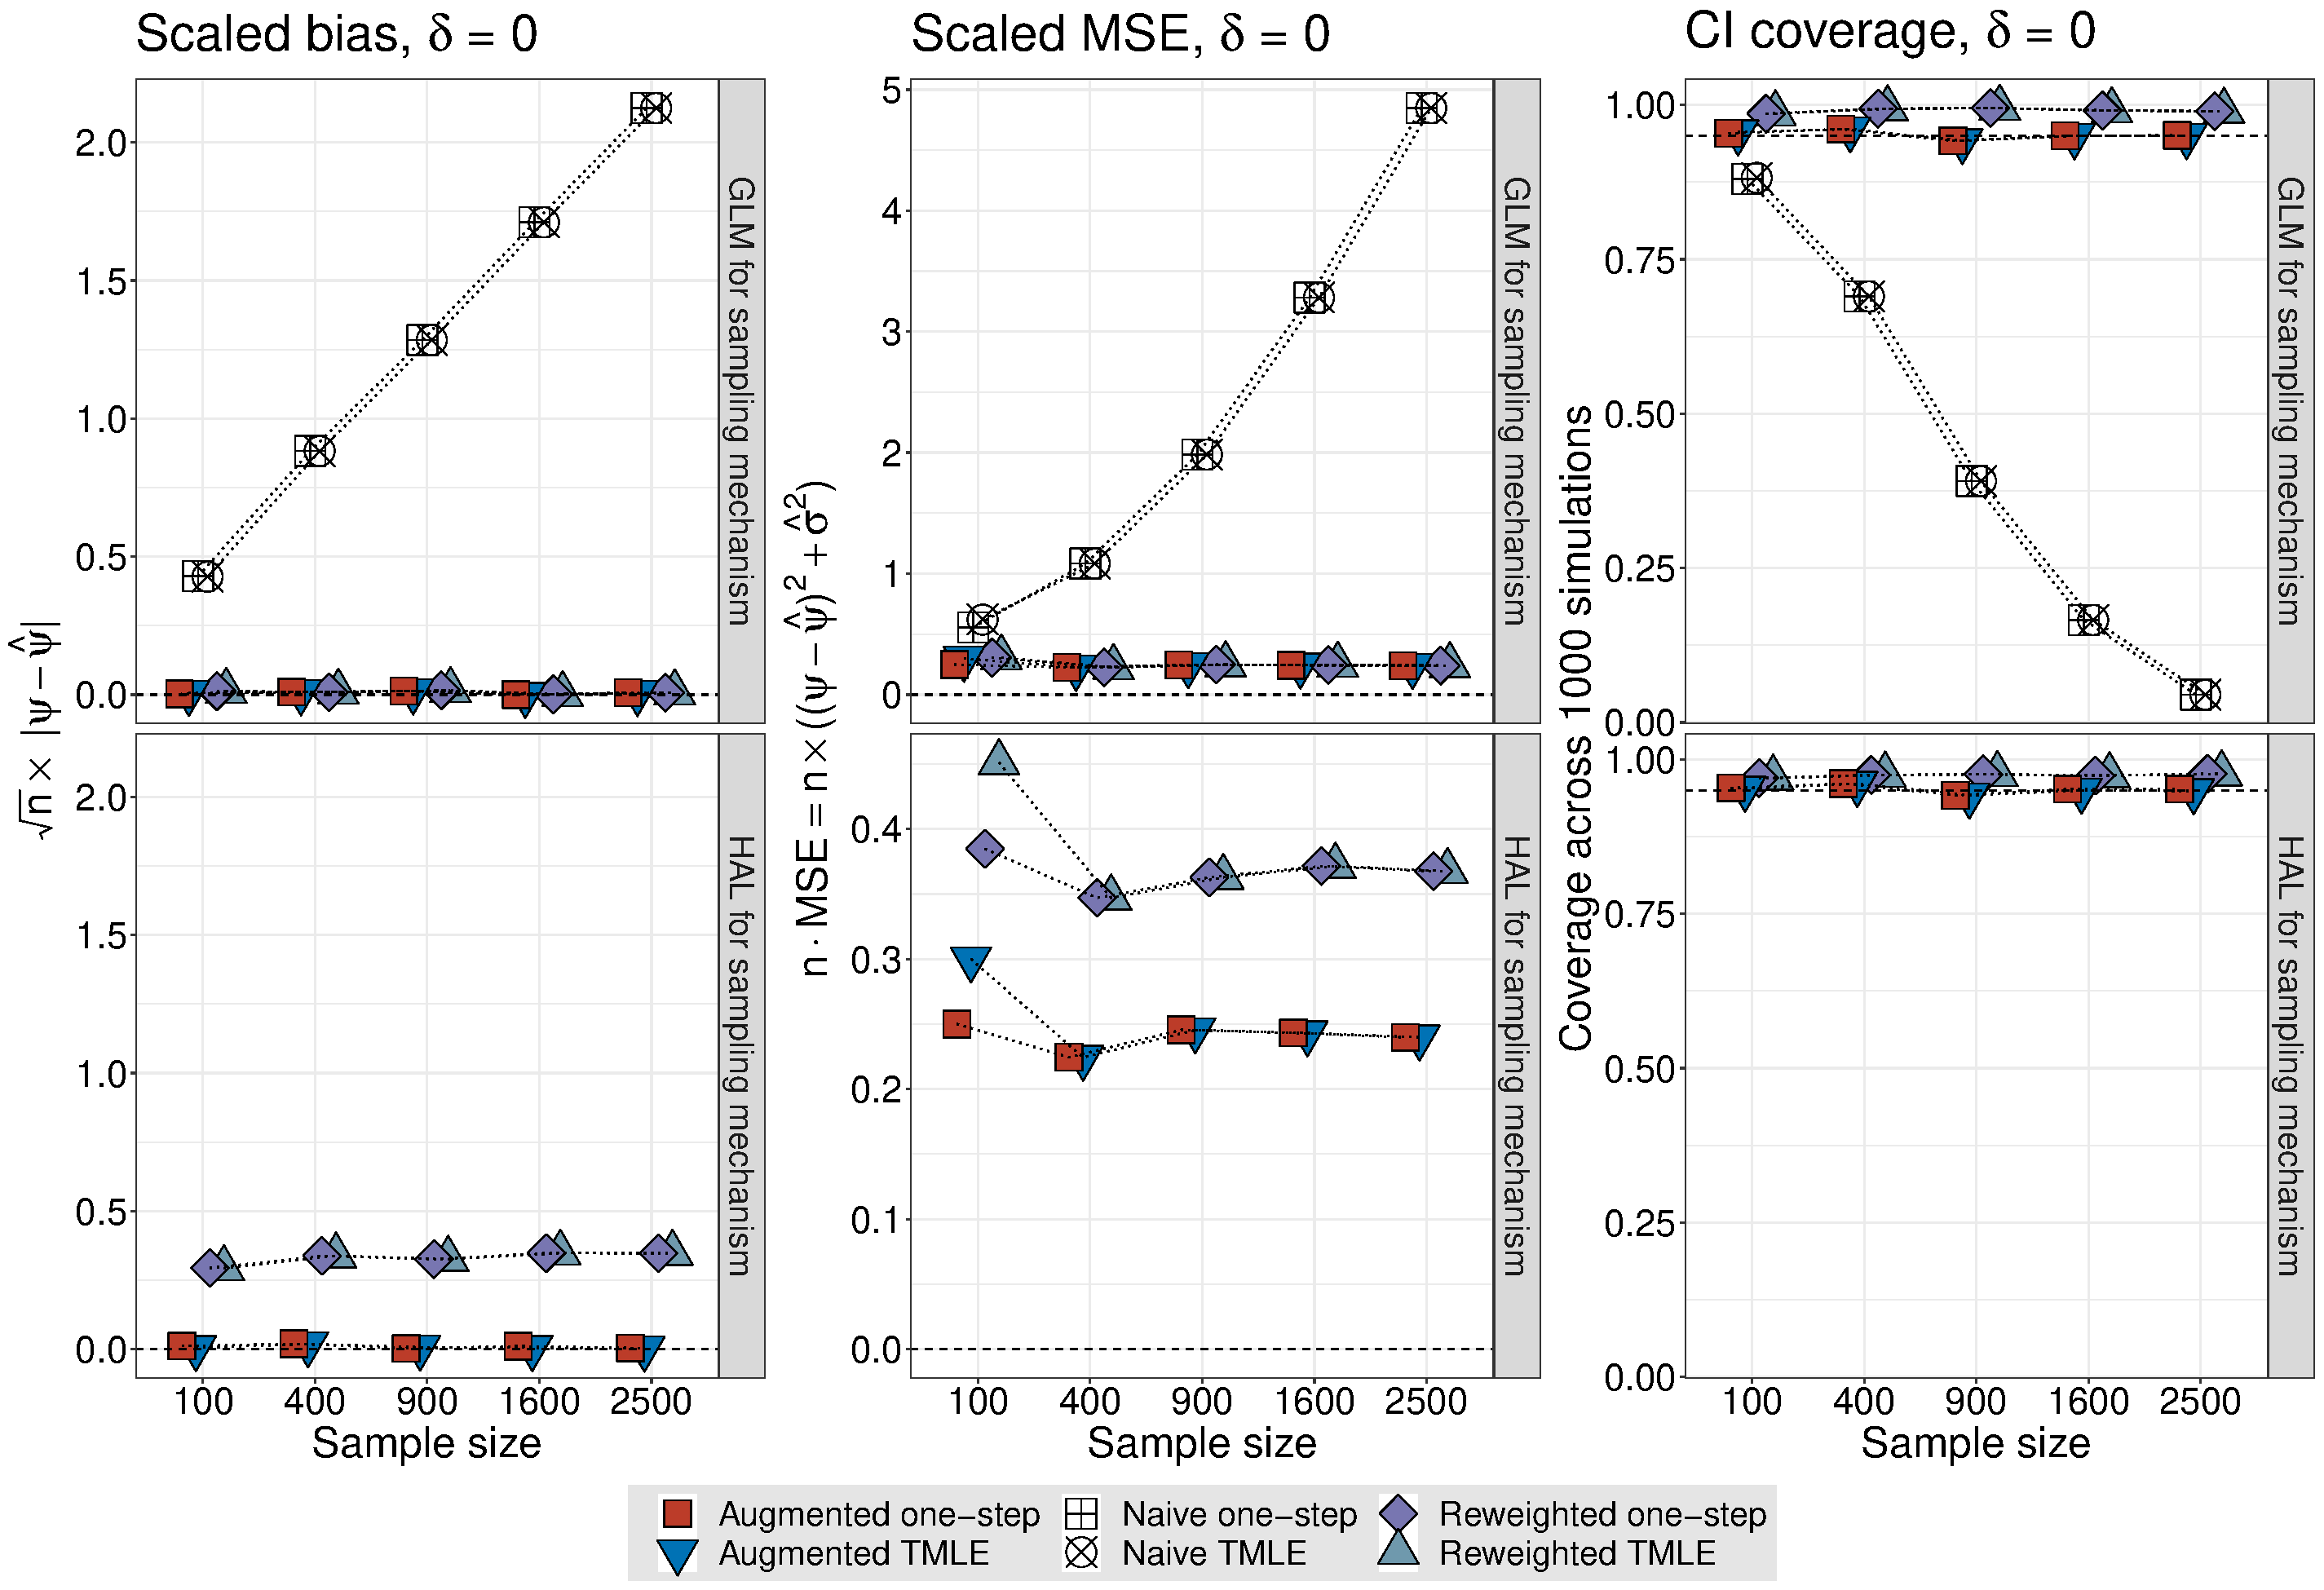
\includegraphics[scale=0.33]{simple_effect_panel_delta_null}
  \caption{Results of numerical simulations comparing six estimation strategies
  for $\psi_{0,\delta}$ for $\delta = 0$.}
  \label{fig:simple_sim_delta_noshift}
\end{figure}

\begin{figure}[H]
  \centering
  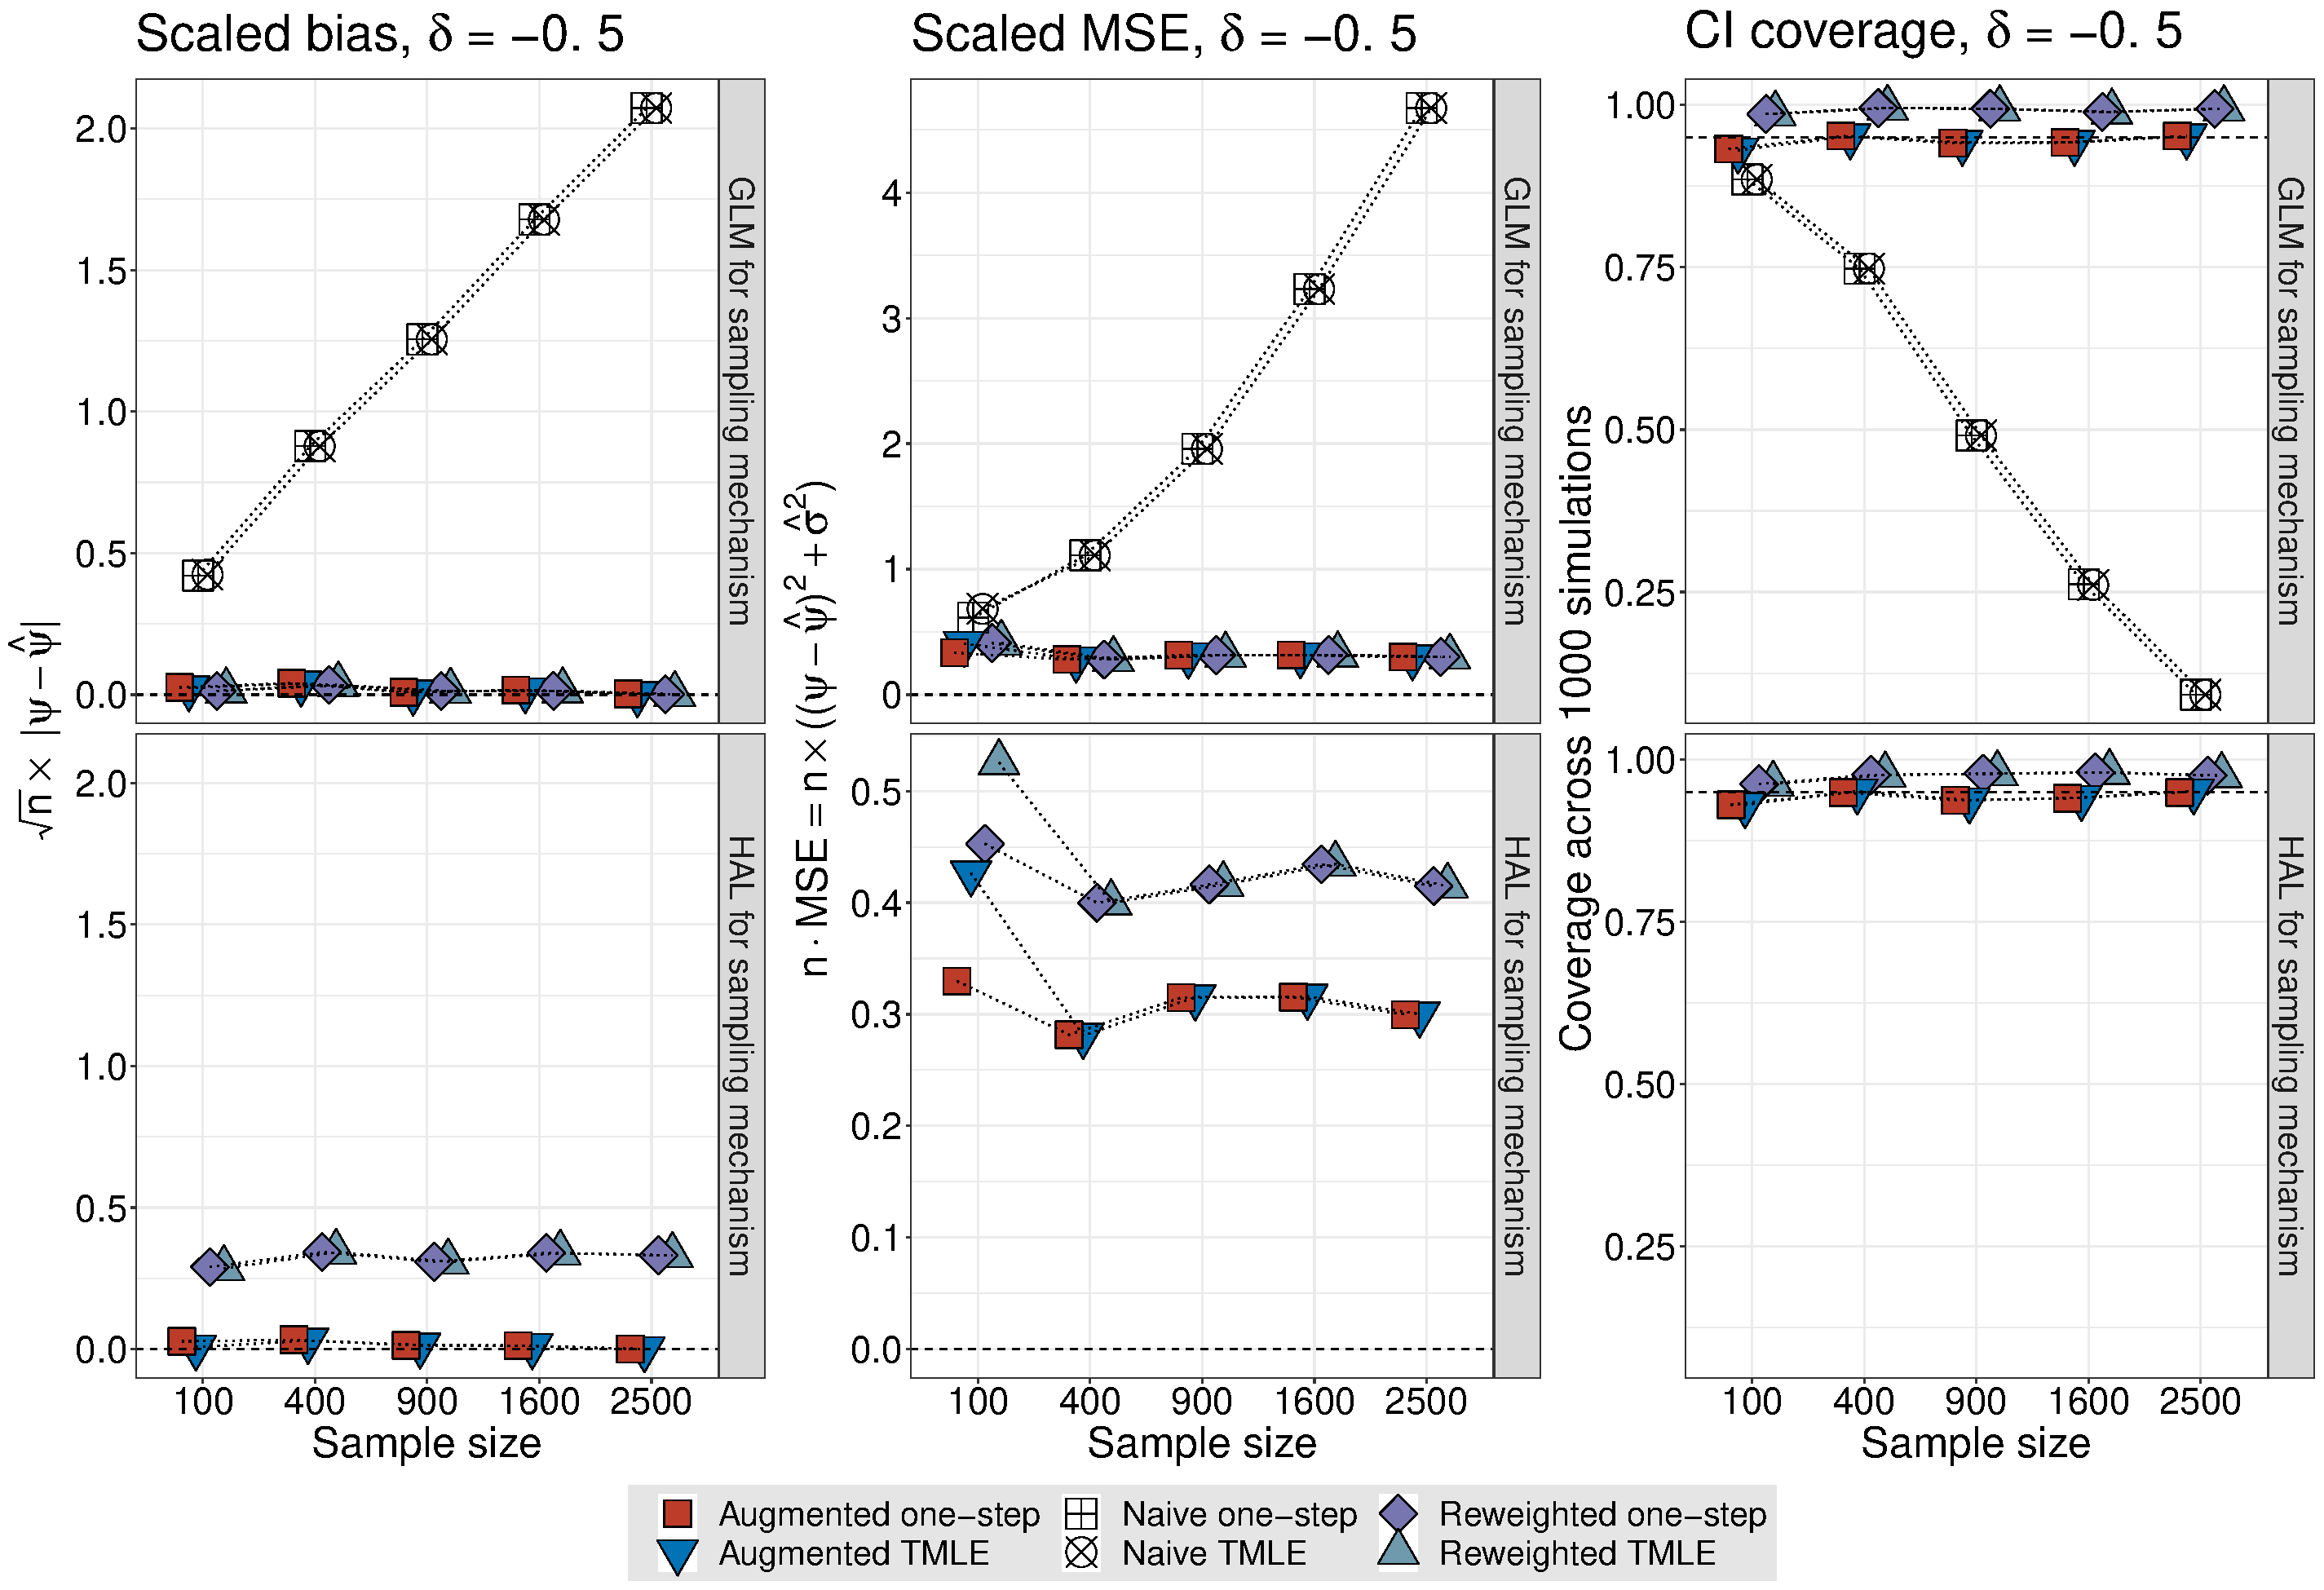
\includegraphics[scale=0.33]{simple_effect_panel_delta_downshift}
  \caption{Results of numerical simulations comparing six estimation strategies
  for $\psi_{0,\delta}$ for $\delta = -0.5$.}
  \label{fig:simple_sim_delta_downshift}
\end{figure}

Both the reweighted estimators of~\citet{rose2011targeted2sd} and our augmented
estimators display the expected level of performance when the sampling mechanism
is estimated via a correctly specified parametric model, standing out against
the performance of their unadjusted counterparts. As in the case of $\delta
= 0.5$, the reweighted estimators display coverage exceeding the desired 95\%
level, while their augmented analogs cover at exactly the nominal level. This
suggests again that the reweighted estimators exhibit an inflated variance
relative to that of our augmented estimators. The lower panel of each figure
visualizes differences in the performance of the estimators when the sampling
mechanism is estimated flexibly via HAL. These results reveal a significant
discrepancy in the performance of the reweighted and augmented estimators, with
our augmented one-step and TML estimators outperforming their reweighted
counterparts in terms of $\sqrt{n}$-bias, $n$-MSE, and coverage. In this second
case, we note that the TML estimators appear to exhibit a small degree of
estimation instability at $n = 100$, displaying larger $n$-MSE in both the
reweighted and augmented variants. We conjecture that this performance is due to
an instability induced by the targeting procedure --- in practice, this could be
ameliorated by alterations to the convergence criterion. Overall, the results of
these numerical investigations do not differ substantially from those presented
in section~\ref{sim}, establishing that our augmented estimators improve
upon alternative estimation strategies when nonparametric estimation of
$g_{0,C}$ is performed.

\subsubsection{Simulation \#2a: Comparing estimators in a scenario based on
  the HVTN 505 trial}\label{hvtn_sim}

For use in real data analysis, we examine only our augmented one-step and TML
estimators. We used the HVTN data to calibrate the following data-generating
mechanism:
\begin{align*}
  W_1 & \sim \mbox{Normal}(26.6, 5.7);
  W_2 \sim \text{Poisson}(40);
  W_3 \sim \bern(0.4);
  W_4 \sim \bern(0.3) \\
  A \mid W & \sim \mbox{Normal}(-1.37 + 0.004 W_1 + 0.015 W_2 + 0.05 W_3 +
    0.25 W_4, 0.2^2)\\
  Y \mid A, W & \sim \bern \left(\expit (-2.9 - 0.0013 W_1 - 0.0016 W_2 +
    0.0678 W_3 + 0.039 W_4 - 0.033 A) \right) \\
  C \mid Y, W & \sim
    \begin{cases}
      \bern \left(\expit (-2.45 - 0.027 W_1 + 0.012 W_2 + 0.39 W_3
      + 0.166 W_4) \right), & Y = 0 \\ 1, & Y = 1
    \end{cases} \ .
\end{align*}
Here, each of the structural equations were generated by fitting parametric
linear or logistic models for $\E[A \mid W]$, $\E[Y \mid A, W]$ and $\E[C \mid
Y = 0, W]$, the means of the CD4+ immunogenic marker, HIV-1 infection risk at
month 24, and probability of inclusion in the second-phase sample, respectively.
Meanwhile, the forms of $W_1, \ldots W_4$ were based on examination of the
empirical distributions of the relevant baseline covariates. Specifically, with
respect to the data from the HVTN 505 trial, $W_1$ mimics BMI, $W_2$ is based on
participants' age, $W_3$ is a binarized clinical behavioral risk score for HIV-1
infection, and $W_4$ behaves as the binarized race/ethnicity. For consistency
with the observed rate of HIV infection in the HVTN 505 trial, the outcome was
made to have a relatively rare event rate, with $\prob(Y = 1 \mid A, W) \approx
0.059$. We considered a setting where we observed $n = 1400$
i.i.d.~observations, approximately matching the sample size of the vaccinated
arm in HVTN 505. Estimator performance was assessed and reported by aggregating
across 1000 repetitions. Under this data-generating mechanism, the true
parameter values were approximated as $\psi_{0,\delta} = \{0.0627, 0.0617,
0.0609, 0.0598, 0.0589, \allowbreak 0.0580, 0.0571, 0.0561, 0.0554\}$ for
$\delta \in \{-2.0, -1.5, -1.0, \allowbreak -0.5, 0.0, 0.5, 1.0, 1.5, 2.0\}$,
respectively. An analogous setting, in which the effect of exposure on the
outcome was removed, yielded similar results; these are presented in the
\href{sm}{Supplementary Materials}.

The proposed estimators were constructed by using the highly adaptive lasso to
estimate the sampling mechanism $g_{n,C}$, the exposure mechanism $q_{n,A}$, the
outcome mechanism $\overline{Q}_{n,Y}$, and the pseudo-outcome regression $G_n$.
We compared the proposed one-step and TML estimators in terms of their bias,
MSE, and coverage of 95\% confidence intervals, summarizing the results in
Figure~\ref{fig:hvtn_sim_moderate}.
\begin{figure}[H]
  \centering
  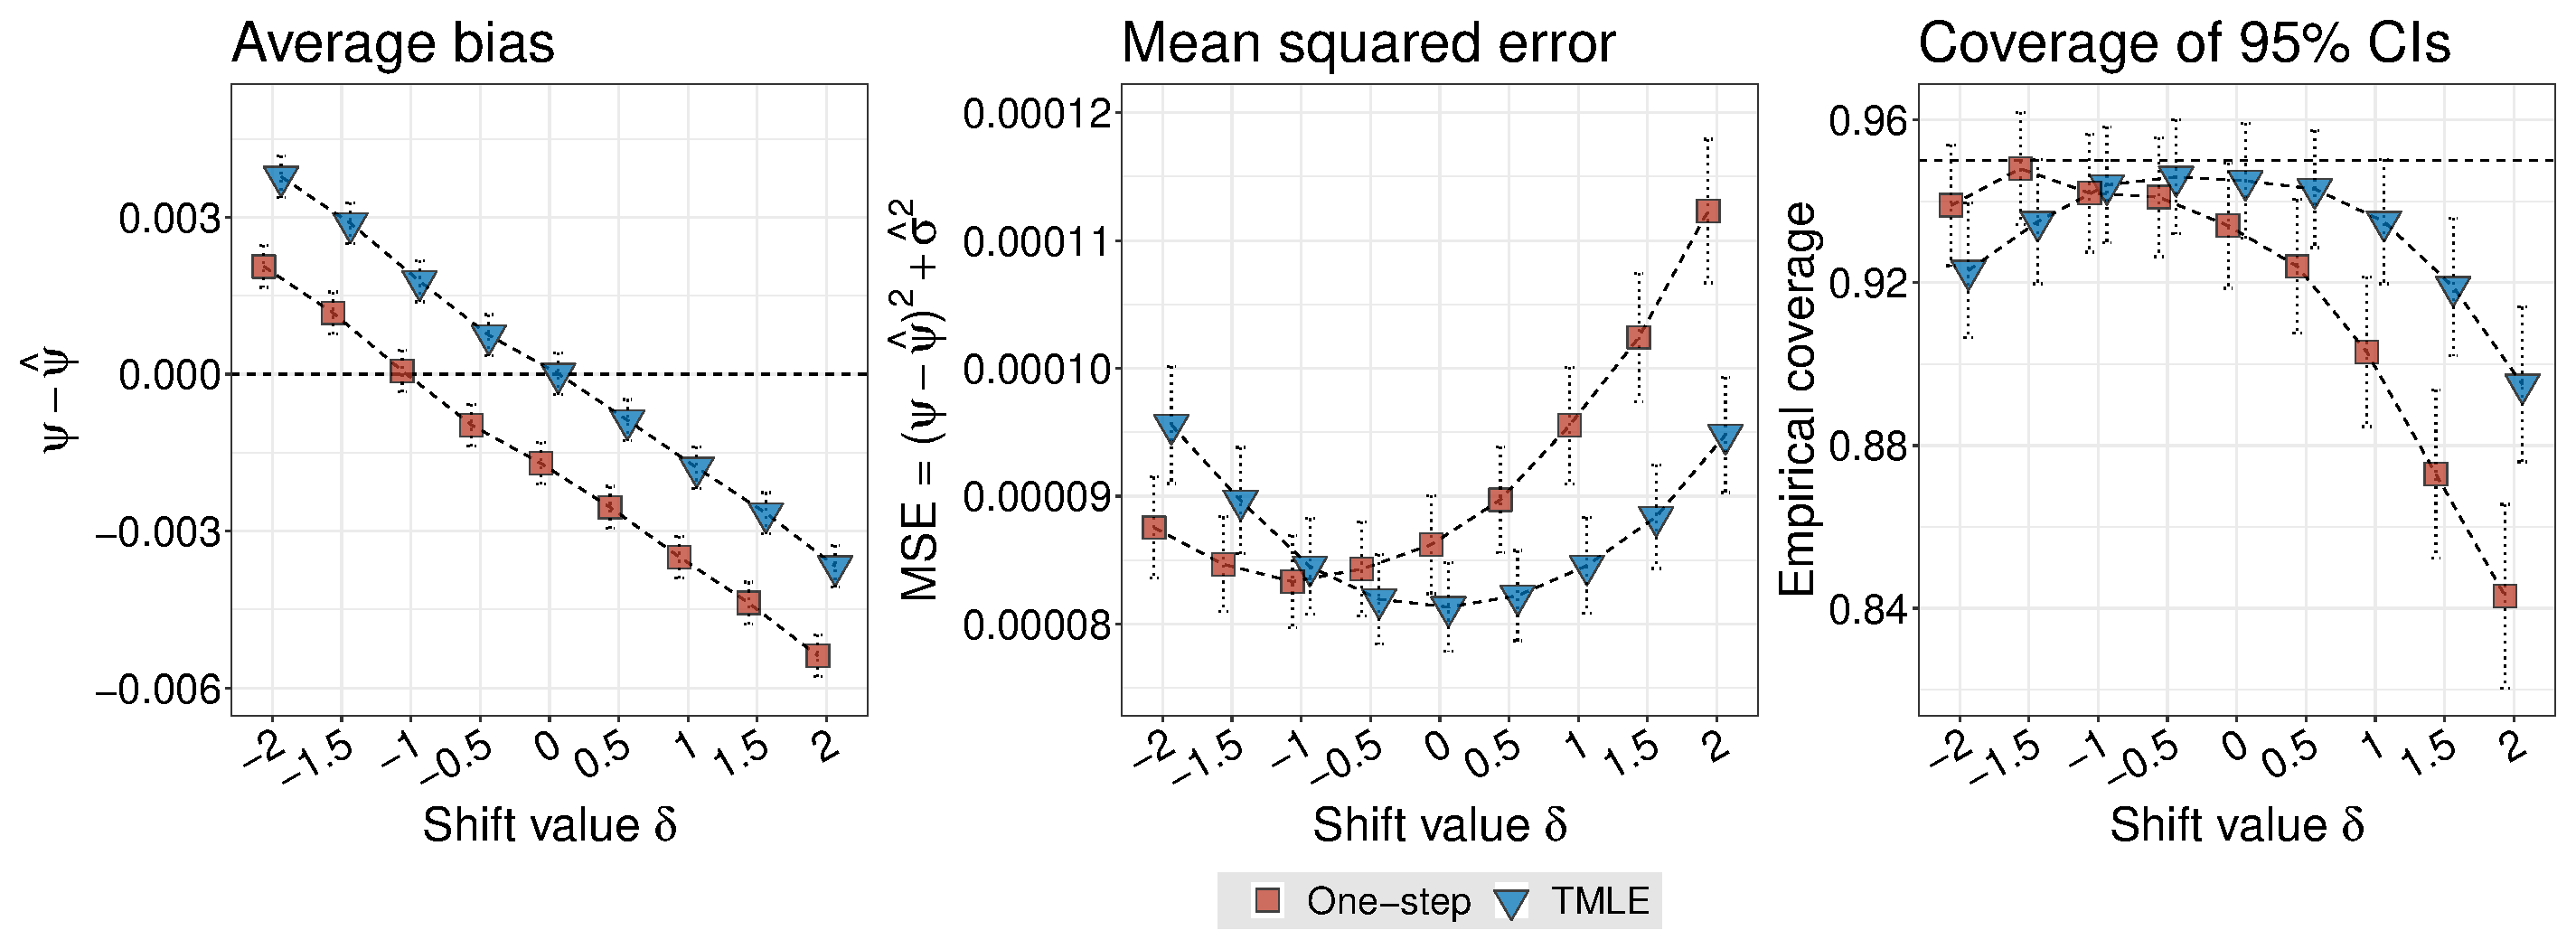
\includegraphics[scale=0.35]{hvtn505_moderate_panel}
  \caption{Results of numerical simulations comparing our two proposed
  estimators of $\psi_{0,\delta}$ for a grid of $\delta$, across 1000 Monte
  Carlo simulations at $n = 1400$.}
  \label{fig:hvtn_sim_moderate}
\end{figure}

%Primarily, the aim of this simulation study is to ascertain whether our
%augmented estimators would perform adequately in a setting similar to our
%motivating HVTN 505 trial. \db{Move up, move up} In contrast to the case of the
%simulation scheme described in section~\ref{simple_sim}, all nuisance parameters
%are estimated only via nonparametric HAL regression --- in this way, we ensure
%that the conditions of our theoretical results are satisfied. An initial
%estimator of the outcome mechanism $\overline{Q}_{n,Y}$ is based on a HAL
%classification model, while the initial estimator of the exposure mechanism
%$q_{n,A}$ is constructed via our HAL-based conditional density estimator
%(described in section~\ref{est_nuisance_param}). Just as with the augmented
%estimators featured in the lower panel of
%Figure~\ref{fig:simple_sim_delta_upshift}, the sampling mechanism $g_{n,C}$ and
%the pseudo-outcome regression $G_n$ were estimated using distinct HAL
%regressions.

Inspection of the bias and MSE indicates that both of our proposed estimators
display adequate performance, with small finite-sample bias and mean squared
error. In terms of bias, the TML estimator outperforms the one-step at $\delta
\geq -0.5$ while the one-step provides better performance at $\delta \leq -0.5$.
Given the exceedingly small scale of the bias, we conclude this to be
a particularity of this data-generating mechanism, not to be used as a guiding
principle in practice. The bias appears to dominate the MSE, with the parabolic
forms of the MSE curves having their respective minima at points at which each
of the estimators is unbiased. Here, the two estimators achieve comparable
performance at $\delta \leq 0$ but the TML estimator outperforms the one-step at
other values of $\delta$. Similarly, in terms of empirical coverage, both
estimators provide coverage near the nominal rate for $\delta \leq 0.5$ but the
performance of the TML estimator suffers less at larger $\delta$. Importantly,
we note that coverage at the nominal rate is only to be expected asymptotically
and is not guarateed by theory in the finite-sample setting presently under
consideration. From these numerical investigations, we concluded that our
augmented estimators are both well-suited to estimating $\psi_{0,\delta}$ in the
context of a re-analysis of data from the HVTN 505 trial.

\subsubsection{Simulation \#2b: Comparing estimators in a scenario like
HVTN 505, without effect of treatment}\label{sim2_supp}

To further assess the performance of our augmented estimators in a scenario like
the HVTN 505 trial, we replace the structural equation for the outcome $Y$ with
a draw from the Bernoulli distribution parameterized as $\bern (p = \expit(-2.8
- 0.0013 W_1 - 0.0016 W_2 + 0.0678 W_3 + 0.039 W_4))$ to achieve a setting in
which there is no effect of the treatment on the outcome. In this case, the
outcome process is relatively rare, with $\prob(Y = 1 \mid A, W) \approx
0.053$. The structural equations for other components of the observed data $O$
are unaltered. In this setting, the true parameter value was approximated to
be $\psi_{0,\delta} = 0.0526$ regardless of the value of $\delta$. We present
the results of assessing our augmented estimators in
Figure~\ref{fig:hvtn_sim_null}.
\begin{figure}[H]
  \centering
  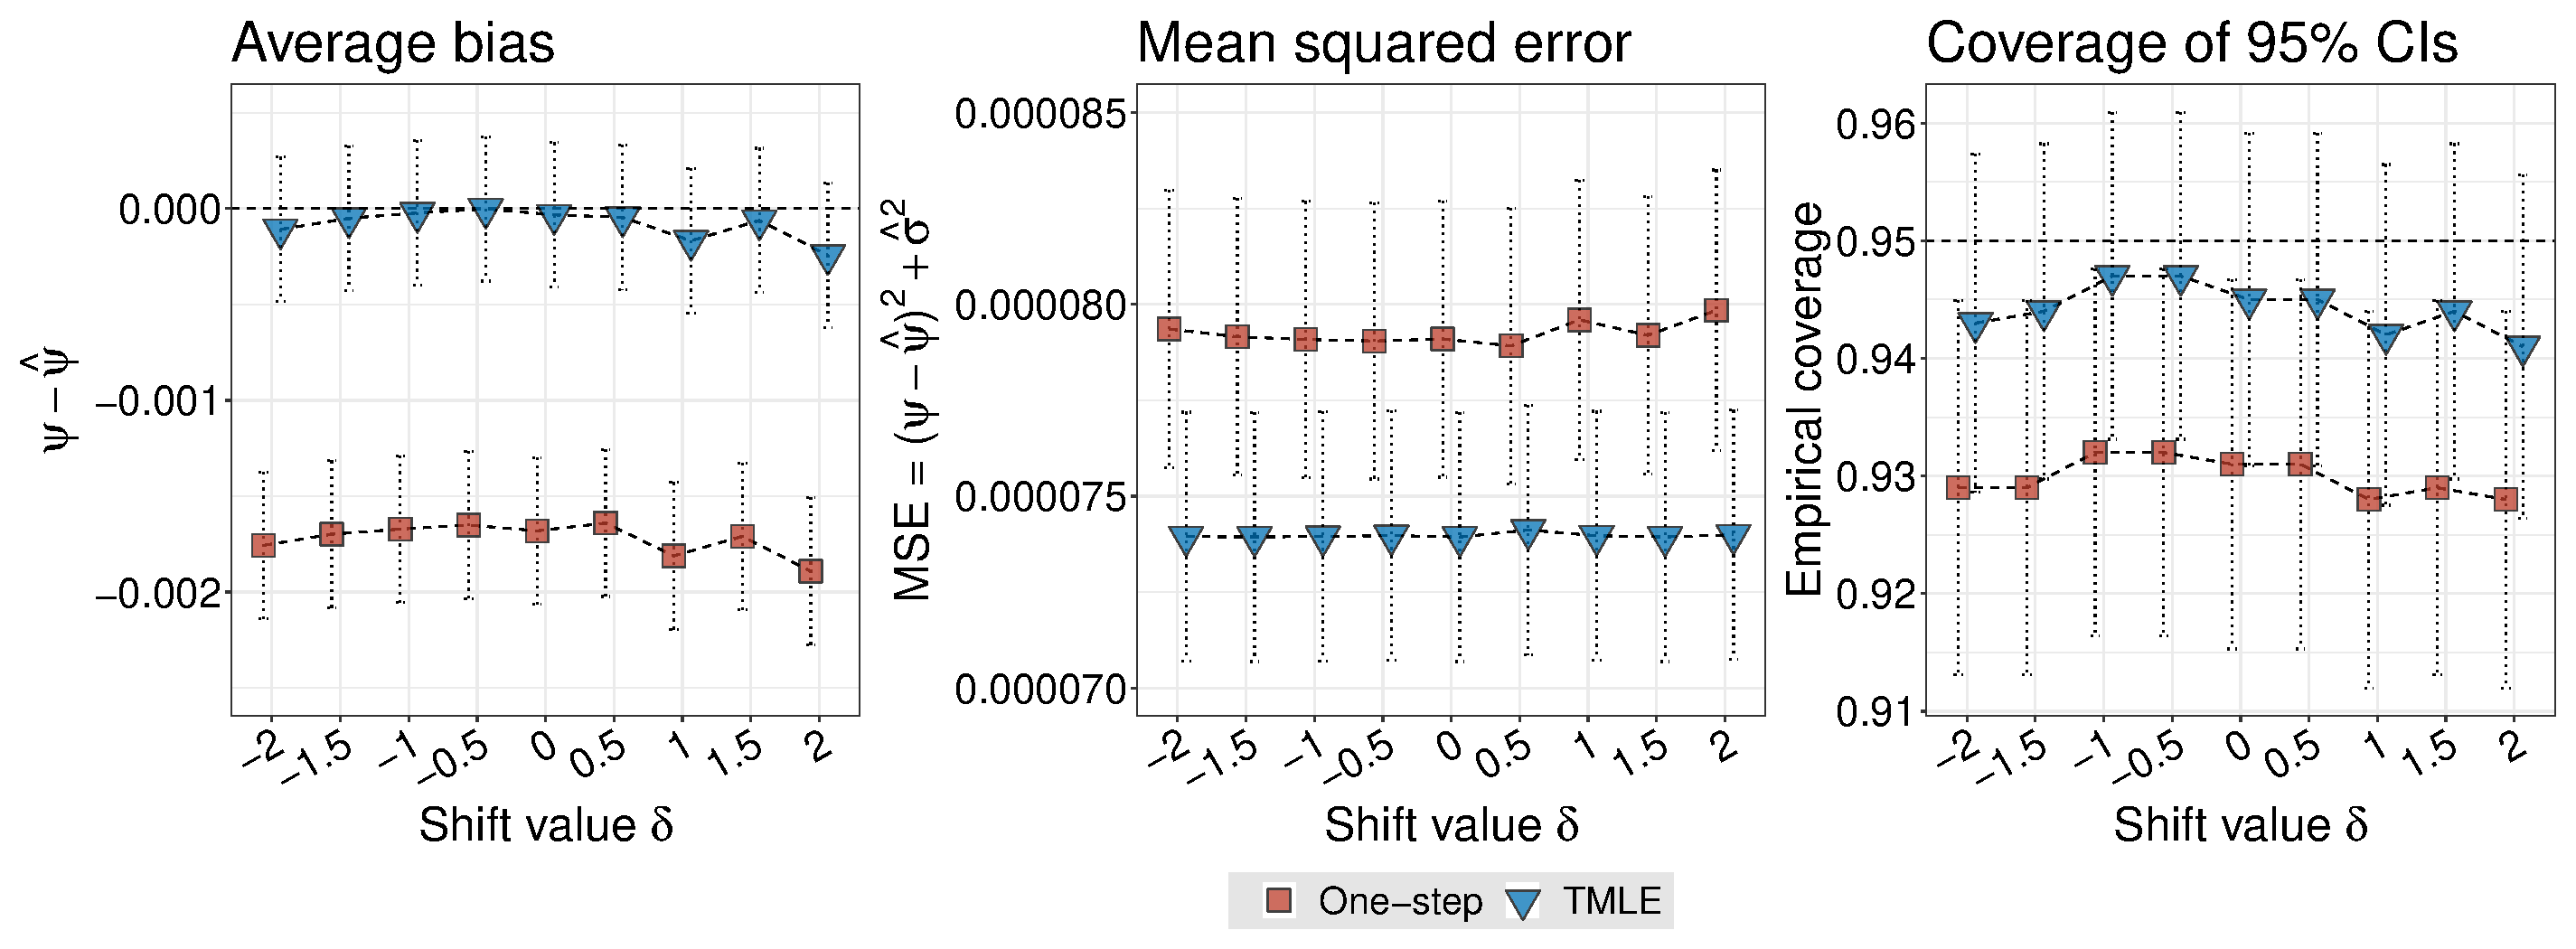
\includegraphics[scale=0.33]{hvtn505_null_panel}
  \caption{Results of numerical simulations comparing our two proposed
     estimators of $\psi_{0,\delta}$ for a grid of $\delta$, across 1000 Monte
     Carlo simulations at $n = 1400$.}
 \label{fig:hvtn_sim_null}
\end{figure}

As the ground truth of the effect of shifting the post-vaccination activity of
the CD4+ and CD8+ immunogenic markers on the risk of HIV-1 infection is unknown
in the HVTN 505 trial, we assess our estimators in this scenario so as to be
sure of there performance when no effect of treatment is present. Estimation of
all nuisance parameters is performed using exactly the same techniques outlined
previously in section~\ref{hvtn_sim}.

In terms of bias and MSE, our proposed estimators display adequate performance.
With respect to both metrics, the TML estimator outperforms the one-step
uniformly in $\delta$, though both estimators display extremely low bias and
MSE. In terms of the coverage of 95\% confidence intervals, the TML estimator
again outperforms the one-step estimator, though only very slightly. Unlike the
results presented in section~\ref{hvtn_sim}, the performance of the estimators,
in terms of all three metrics, appears stable across $\delta$, providing further
evidence that the phenomenon appearing in that numerical study was
a particularity of the effect of $A$ on $Y$ under this data-generating
mechanism. The improved performance of the TML estimator over the one-step
estimator is in line with prior demonstrations of the enhanced finite-sample
performance of TML estimators~\citep{vdl2011targeted}. As with the numerical
investigations presented in section~\ref{hvtn_sim}, these results suggest that
our augmented estimators will perform well enough to allow accurate estimation
of $\psi_{0,\delta}$ when applied to data from the HVTN 505 trial.

\subsection{Super Learner ensemble models for $\overline{Q}_{n,Y}$ in the HVTN
  505 data analysis}\label{hvtn_sl_details}

As noted in section~\ref{application}, for both the CD4+ and CD8+ analyses,
the estimated outcome mechanism $\overline{Q}_{n,Y}$ was constructed from an
ensemble model based on the super learner algorithm~\citep{vdl2007super}. The
cross-validation selector that forms the basis of the super learner has been
shown to exhibit unique theoretical guarantees, including asymptotic equivalence
to the oracle selector~\citep{vdl2004asymptotic, vdl2006cross, vdl2006oracle},
that make its use preferable over other ensemble learning approaches.

A rich library of candidate classification algorithms was considered in the
super learner ensemble model for $\overline{Q}_{n,Y}$. These included
$\ell_1$-penalized lasso regression~\citep{tibshirani1996regression,
friedman2009glmnet}; $\ell_2$-penalized ridge regression
\citep{tikhonov1977solutions,hoerl1970ridge,friedman2009glmnet}; three elastic
net regressions weighting the $\ell_1$ penalty at $\alpha \in \{0.25, 0.50,
0.75\}$ and the $\ell_2$ penaly at
$(1-\alpha)$~\citep{zou2003regression,friedman2009glmnet}; random
forests~\citep{breiman2001random} with 50, 100, and 500 trees based on its
implementation in the \texttt{ranger} \texttt{R}
package~\citep{wright2017ranger}; extreme gradient boosted trees with 20, 50,
100, and 300 fitting iterations~\citep{chen2016xgboost}; multivariate adaptive
polynomial spline regression~\citep{kooperberg1997polychotomous,stone1994use};
multivariate adaptive regression splines~\citep{friedman1991multivariate};
generalized linear models with Bayesian priors on parameters; a multilayer
perceptron~\citep{rosenblatt1961principles}; and the highly adaptive
lasso~\citep{vdl2017generally,benkeser2016highly,coyle2019hal9001}. The
implementation of the super learner algorithm in the \texttt{sl3} \texttt{R}
package~\citep{coyle2020sl3} was used, and weights assigned to each learning
algorithm by the super learner are given in Tables~\ref{tab:cd4_sl_coefs}
and~\ref{tab:cd8_sl_coefs} for the CD4+ and CD8+ analyses, respectively.

\begin{table}[H]
\caption{\label{tab:cd4_sl_coefs} Weights and risk estimates assigned to each
  individual learning algorithm in the ensemble model for $\overline{Q}_{n,Y}$
  used in the reported re-analysis of the CD4+ immunogenic marker.}
\centering
\begin{tabular}[t]{l|r|r|r|r}
\hline
Learner & Weight & Min. Fold Risk & Mean CV-Risk & Max. Fold Risk\\
\hline
Ridge ($\ell_2$ penalized) & 0.147 & 0.015 & 0.036 & 0.052\\
\hline
Lasso ($\ell_1$ penalized) & 0.000 & 0.015 & 0.036 & 0.052\\
\hline
Elastic net ($\alpha = 0.25$) & 0.116 & 0.015 & 0.036 & 0.051\\
\hline
Elastic net ($\alpha = 0.50$) & 0.000 & 0.015 & 0.036 & 0.051\\
\hline
Elastic net ($\alpha = 0.75$) & 0.181 & 0.015 & 0.036 & 0.051\\
\hline
Random forest (50 trees) & 0.000 & 0.062 & 0.097 & 0.173\\
\hline
Random forest (100 trees) & 0.000 & 0.050 & 0.093 & 0.153\\
\hline
Random forest (500 trees) & 0.000 & 0.061 & 0.093 & 0.158\\
\hline
xgboost(20 iterations) & 0.000 & 0.012 & 0.072 & 0.165\\
\hline
xgboost(50 iterations) & 0.000 & 0.012 & 0.080 & 0.181\\
\hline
xgboost(100 iterations) & 0.010 & 0.013 & 0.088 & 0.192\\
\hline
xgboost(500 iterations) & 0.000 & 0.012 & 0.098 & 0.204\\
\hline
Highly adaptive lasso (default) & 0.014 & 0.064 & 0.074 & 0.084\\
\hline
Highly adaptive lasso (custom) & 0.000 & 0.066 & 0.075 & 0.084\\
\hline
Multivariate adaptive regression splines & 0.000 & 0.050 & 0.086 & 0.131\\
\hline
Polynomial spline regression & 0.208 & 0.015 & 0.036 & 0.053\\
\hline
Multilayer perceptron network & 0.000 & 0.015 & 0.037 & 0.055\\
\hline
GLM with Bayesian priors & 0.323 & 0.015 & 0.036 & 0.051\\
\hline
Super Learner & 1.000 & --- & --- & ---\\
\hline
\end{tabular}
\end{table}

In the super learner ensemble model for the outcome regression in the CD4+
analysis, the three best learning algorithms were a GLM with Bayesian priors on
parameter estimates, a polynomial spline regression model, and an elastic net
regression model that favored the $\ell_1$ (lasso) penalty over the $\ell_2$
(ridge) penalty. Another variant of elastic net regression, which favored the
$\ell_2$ penalty over the $\ell_1$ penalty, and ridge regression were also given
nontrivial weights in the ensemble model. A variant of extreme gradient boosting
and the highly adaptive lasso received low weights, while all other candidate
algorithms in the library were assigned weights of zero.

\begin{table}[H]
\caption{\label{tab:cd8_sl_coefs} Weights and risk estimates assigned to each
  individual learning algorithm in the ensemble model for $\overline{Q}_{n,Y}$
  used in the reported re-analysis of the CD8+ immunogenic marker.}
\centering
\begin{tabular}[t]{l|r|r|r|r}
\hline
Learner & Weight & Min. Fold Risk & Mean CV-Risk & Max. Fold Risk\\
\hline
Ridge ($\ell_2$ penalized) & 0.161 & 0.013 & 0.037 & 0.075\\
\hline
Lasso ($\ell_1$ penalized) & 0.161 & 0.011 & 0.037 & 0.075\\
\hline
Elastic net ($\alpha = 0.25$) & 0.003 & 0.012 & 0.037 & 0.075\\
\hline
Elastic net ($\alpha = 0.50$) & 0.000 & 0.014 & 0.037 & 0.076\\
\hline
Elastic net ($\alpha = 0.75$) & 0.131 & 0.014 & 0.037 & 0.074\\
\hline
Random forest (50 trees) & 0.090 & 0.053 & 0.088 & 0.129\\
\hline
Random forest (100 trees) & 0.055 & 0.048 & 0.089 & 0.136\\
\hline
Random forest (500 trees) & 0.119 & 0.049 & 0.088 & 0.127\\
\hline
xgboost(20 iterations) & 0.000 & 0.043 & 0.064 & 0.112\\
\hline
xgboost(50 iterations) & 0.000 & 0.036 & 0.074 & 0.128\\
\hline
xgboost (100 iterations & 0.000 & 0.031 & 0.076 & 0.134\\
\hline
xgboost (300 iterations) & 0.000 & 0.029 & 0.086 & 0.146\\
\hline
Highly adaptive lasso (default) & 0.000 & 0.046 & 0.078 & 0.115\\
\hline
Highly adaptive lasso (custom) & 0.000 & 0.044 & 0.078 & 0.132\\
\hline
Multivariate adaptive regression splines & 0.000 & 0.029 & 0.100 & 0.159\\
\hline
Polynomial spline regression & 0.000 & 0.015 & 0.040 & 0.080\\
\hline
Multilayer perceptron network & 0.067 & 0.007 & 0.040 & 0.085\\
\hline
GLM with Bayesian priors & 0.214 & 0.016 & 0.037 & 0.073\\
\hline
Super Learner & 1.000 & --- & --- & ---\\
\hline
\end{tabular}
\end{table}

In the CD8+ analysis, the three best learning algorithms, chosen by the super
learner ensemble model for the outcome regression, were a GLM with Bayesian
priors on parameter estimates, ridge regression, and lasso regression. Other
algorithms that were assigned nontrivial weights included an elastic net
regression model that favored the $\ell_1$ (lasso) penalty over the $\ell_2$
(ridge) penalty and a random forest with 500 trees. A variant of elastic net
regression, random forests with 50 and 100 trees, and a multilayer perceptron
all received low weights, while all other candidate algorithms in the library
were assigned weights of zero.


\chapter{Stochastic Interventional Vaccine Efficacy}\label{three}

\section{Introduction}

The core ideas of Chapter~\ref{two} can form a novel approach to studying immune
correlates of protection --- those immunologic markers \textit{causally}
antagonistic to the process of infection~\citep{plotkin2012nomenclature}. In
vaccine efficacy trials of infectious diseases, such analyses can aid in
developing a more nuanced understanding of the differing roles that immunologic
markers can play in impacting vaccine efficacy and, beyond this, elucidate the
mechanism by which the activities of these markers may afford protection. This
analytic framework quantifies vaccine efficacy as the effect attributable to
shifting (upwards or downwards) the immune response distribution (i.e.,
immunologic marker activity) in vaccinees~\citep{hejazi2020efficient}, revealing
the complex interplay between vaccination, immunologic marker activity, and
infection.

To formalize, let us denote by the random variable $O = (W, A, S, Y)$ the data
collected on a single individual in a randomized vaccine efficacy trial,
where $W$ are clinically relevant baseline risk factors for infection (e.g.,
age, body mass index), $A$ is the randomized assignment to placebo or vaccine,
$S$ is the immune response activity of an antibody of interest, and $Y$ is an
indicator of infection. Throughout, we assume that $S$ is the scalar-valued
activity of a particular antibody, as quantified by an established immunoassay,
and is a candidate immune correlate of protection. In measuring $S$, we further
assume that biological material (e.g., drawn blood) for evaluating the activity
of the immunologic marker is taken at an \textit{a priori}-specificed time
post-vaccination. Since such trials often measure the time-to-infection, the
outcome process is generally a composite time-to-event quantity
$\{\tilde{T} = \min(T_F, T_C), \Delta = \mathbb{I}(T_F < T_C)\}$, where $T_F$
and $T_C$ are the (mutually unobservable) failure and censoring times,
respectively, and $\Delta$ is simply the indicator of observed failure. We
simplify this to $Y \coloneqq \mathbb{I}(\Delta = 1)$ (i.e., observed infection)
by the end of the trial.

Leveraging the framework developed in Chapter~\ref{two}, we formulate and
evaluate vaccine efficacy parameters in the context of efficacy trials of the
vaccines produced to counteract the COVID-19 pandemic. The central goal of this
and related statistical analyses~\citep[e.g.,][]{benkeser2021inference,
gilbert2021assessment} is to derive reliable, parsimonious surrogate
endpoints~\citep{prentice1989surrogate, gilbert2008evaluating} based on the
immunologic marker activity measured by a given immunoassay, effectively
narrowing the set of candidate immune correlates of protection and curbing the
time and resources consumed by vaccine efficacy trials. Alternative techniques
and shared details of the data analytic approach are outlined in the immune
correlates statistical analysis plan of the COVID-19 Vaccine Prevention Network
(CoVPN)~\citep{gilbert2021covpn}. Each of outlined analyses is implemented in
the \texttt{R} programming language~\citep{R}, all publicly available at
\url{https://github.com/CoVPN/correlates_reporting}, which incorporates version
control and continuous integration for automated code checking and analysis
report generation.

\section{Formulating Vaccine Efficacy Parameters}

Taking the outcome of interest $Y$ to be the indicator of a COVID-19 disease
endpoint of interest by a pre-specified time (e.g., $Y \in \{0, 1\}$ by Day 57
post-vaccination), we consider the counterfactual outcome $Y(a,s)$ generated by
a hypothetical intervention setting both the randomized vaccination assignment
(i.e., $A = a$) and the immunologic marker activity (at the specified timepoint)
$S$ to a random draw from an analyst-specified distribution. Consider the shift
$\delta$ to be a hypothetical change in the standardized response activity of
the immunologic marker $S$ in question. In particular, we may conceive of the
effect on risk of a given COVID-19 endpoint of a controlled intervention
shifting the distribution of an immunologic response by $\delta$ units, for
externally specified values of $\delta$. Such interventions on vaccine-induced
immunologic marker activity can be viewed as the hypothetical results of
potential changes to the candidate vaccine, for example, change in dose or
vaccine re-formulation. As the immunologic marker activity at $\delta = 0$
corresponds to that induced by the curent vaccine, we can consider
counterfactual scenarios in which changes to the vaccine result in relatively
heightened (if $\delta > 0$) or muted (if $\delta < 0$) immune response.

To query the counterfactual risk of the COVID-19 endpoint of interest under the
hypothetical modified vaccine, that is, the vaccine inducing immune response $S
+ \delta$ for $\delta \in \mathbb{R}$, we naturally consider the mean of the
counterfactual outcomes of the form $Y(1, S(1) + \delta)$, corresponding to the
risk in vaccinees receiving the hypothetical vaccine. A similar approach, based
on the controlled direct effect~\citep{benkeser2021inference}, evaluates the
effect of an intervention that sets $S = s$ statically, thereby assuming that it
is possible to set the post-intervention immune response value $s$ for
\textit{all individuals in the population}. Unfortunately, this rather stringent
assumption may be unrealistic when $s$ is large and there exist subpopulations
with within which the modified vaccine fails to elicit a strongly immunogenic
response. The stochastic interventional approach presently described makes a far
laxer assumption on the intervention: The intervention need only
shift immune responses relative to the observed value for a given individual,
allowing for individual-specific (or subpopulation-specific) changes in
vaccine-induced immunogenicity.

Under standard identification assumptions~\citep{diaz2012population,
hejazi2020efficient}, such as no unmeasured confounding and positivity,
generally required for all causal analyses, the counterfactual risk
$\E[Y(1, S(1)
+ \delta)]$ is identified by
\begin{equation}\label{eqn:stochintrisk}
  \E[\P(Y = 1 \mid A = 1, S = S + \delta, W = w) \mid A = 1, W] \ .
\end{equation}
By examining this quantity across a range of feasible $\delta$ values provides
insight into the relative contribution of a given immunologic response marker in
preventing the manifestation of the endpoint of interest.
Noting that $\P(Y(0)=1) = \P(Y=1 \mid A=0)$ (in view of vaccine
versus placebo randomization, as given in \citep{gilbert2021assessment}) and
that
this quantity may
be estimated in the same way as for the controlled vaccine efficacy analyses,
we define
stochastic interventional vaccine efficacy (SVE) as
\begin{equation}\label{eqn:sve}
\text{SVE}(\delta) = 1 - \frac{\E[\P(Y = 1 \mid A = 1, S = S + \delta, W = w)
\mid A = 1, W]}{\P(Y(0)=1)} \ .
\end{equation}

\section{Considerations for Statistical Estimation}

\citet{hejazi2020efficient} proposed nonparametric estimators that rely on
estimates of the outcome regression and the conditional density of the immune
response in vaccinated participants. Their estimators efficiently account for
two-phase sampling of immune responses and are implemented in the
\texttt{txshift} package~\citep{hejazi2020txshift-joss} for the \texttt{R}
language and environment for statistical computing~\citep{R}, freely available
through both GitHub at \url{https://github.com/nhejazi/txshift} and the
Comprehensive \texttt{R} Archive Network at
\url{https://CRAN.R-project.org/package=txshift}.

To assess vaccine efficacy against COVID-19 endpoints, we apply these estimators
to several immunologic markers measured at Day 57, controlling for a common set
of baseline risk factors in the interest of alignment with other CoVPN analyses.
For further details on the immunologic markers and risk factors, as well as key
details on study design, we refer the interested reader to the comprehensive
statistical analysis plan of~\citet{gilbert2021covpn}. Similar to the natural
effects approach of \citet{benkeser2021inference}, our implementation leverages
low-dimensional risk factors alongside parametric regression strategies and
flexible conditional density estimation for endpoints with fewer than $100$
observed cases (pooling across trial arms); however, more flexible statistical
learning techniques are employed for modeling the outcome process for endpoints
with a greater number of observed cases.

In particular, conditional density estimates of immune response markers are
based principally on a nonparametric estimation strategy that constructs the
conditional density through estimates of the conditional hazard of the
discretized immune response marker values~\citep{hejazi2020efficient,
hejazi2021haldensify}, as per Algorithm~\ref{alg:pooled_haz_dens} of
Chapter~\ref{one}; this approach is an extension of the proposal
of~\citet{diaz2011super}. A Super Learner ensemble~\citep{vdl2007super} of
variants of this nonparametric conditional density estimator and the
semiparametric location-scale conditional density estimation procedure discussed
in Algorithm~\ref{alg:loc_scale_dens} of Chapter~\ref{one}, as. implemented in
the \texttt{sl3} \texttt{R} package~\citep{coyle2021sl3}. In settings with
limited numbers of case endpoints, the outcome process is modeled as a Super
Learner ensemble of a library of parametric regression
techniques~\citep[per][]{gruber2010application}, while the algorithm library is
augmented with flexible regression techniques --- including, for example, lasso
and ridge regression~\citep{tibshirani1996regression, tikhonov1977solutions,
hoerl1970ridge}, elastic net regression~\citep{zou2003regression,
friedman2009glmnet}, random forests~\citep{breiman2001random, wright2017ranger},
extreme gradient boosting machines~\citep{chen2016xgboost}, multivariate
adaptive polynomial and regression splines~\citep{friedman1991multivariate,
stone1994use, kooperberg1997polychotomous}, and the highly adaptive
lasso~\citep{vdl2017generally, benkeser2016highly, hejazi2020hal9001,
coyle2021hal9001} --- as the number of case endpoints grows. The choice of
algorithm library is coordinated across the CoVPN correlates of protection
analyses~\citep{gilbert2021covpn}.

Output of the analyses will be presented as point and 95\% confidence interval
estimates of $\E[Y(1, S(1) + \delta)]$ and of $\text{SVE}(\delta)$ over the
values of $s$ for each of the Day 57 immunologic markers, for each of a range of
$\delta$ spanning the interval $[-1, 1]$ on the standard unit scale for each
immunologic marker. As with related analyses, in the context of data from
real-world COVID-19 trials, these analyses are to be carried out only if
diagnostics support plausibility of the positivity assumption. Notably, however,
the positivity assumption for the stochastic interventional effects is unique.
Where the positivity assumption for effects defined by static interventions
requires a positive probability of treatment assignment across \textit{all
strata} defined by baseline factors (i.e., that a discretized immune response
value be possible regardless of baseline factors), the positivity assumption of
our effects is
\begin{equation*}
  s_i \in \mathcal{S} \implies s_i + \delta \in \mathcal{S} \mid A = 1, W = w
\end{equation*}
\noindent for all $w \in \mathcal{W}$ and $i = 1, \ldots n$. In particular, this
positivity assumption does not require that the post-intervention exposure
density, $q_{0,S}(S - \delta \mid A = 1, W)$, place mass across all strata
defined by $W$. Instead, it requires that the post-intervention exposure
mechanism be bounded, that is,
\begin{equation*}
  \P \{q_{0,S}(S - \delta \mid A = 1, W) / q_{0,S}(S \mid A = 1, W) > 0 \} = 1,
\end{equation*}
\noindent which may be readily satisfied by a suitable choice of $\delta$.

Importantly, the static intervention approach may require consideration of
counterfactual variables that are scientifically unrealistic. Namely, it may be
inconceivable to imagine a world where every participant exhibits high immune
responses, given the phenotypic variability of participants' immune systems.
This too may be resolved by considering an intervention indexed not by $\delta$
but by $\delta(W)$, that is, one in which the choice of the shift is itself
a function of the baseline covariates $W$~\citep{hejazi2020efficient,
diaz2012population, haneuse2013estimation, diaz2018stochastic}.

\section{Application to the COVID-19 Pandemic}

We estimate the counterfactual mean of symptomatic COVID-19 infection under
posited shifts in the measured activity levels of each of immunologic markers
that are \emph{candidate} mechanistic correlates of protection (mCoP), as
defined by the aims of the CoVPN statistical analysis
plan~\citep{gilbert2021covpn}. By shifting the \emph{standardized} immunologic
activity levels by standard unit shifts along the grid $\{-1, -0.5, 0, 0.5,
1\}$, we can assess the degree to which vaccines that modulate mCoP immunologic
marker activity to these modified levels could mitigate symptomatic COVID-19
infection in terms of both counterfactual stochastic interventional risk and
vaccine efficacy (VE). In the sequel, we demonstrate our approach using the Day
57 activity of the spike protein binding and pseudo-neutralizing antibodies.

\begin{figure}[H]
  \centering
  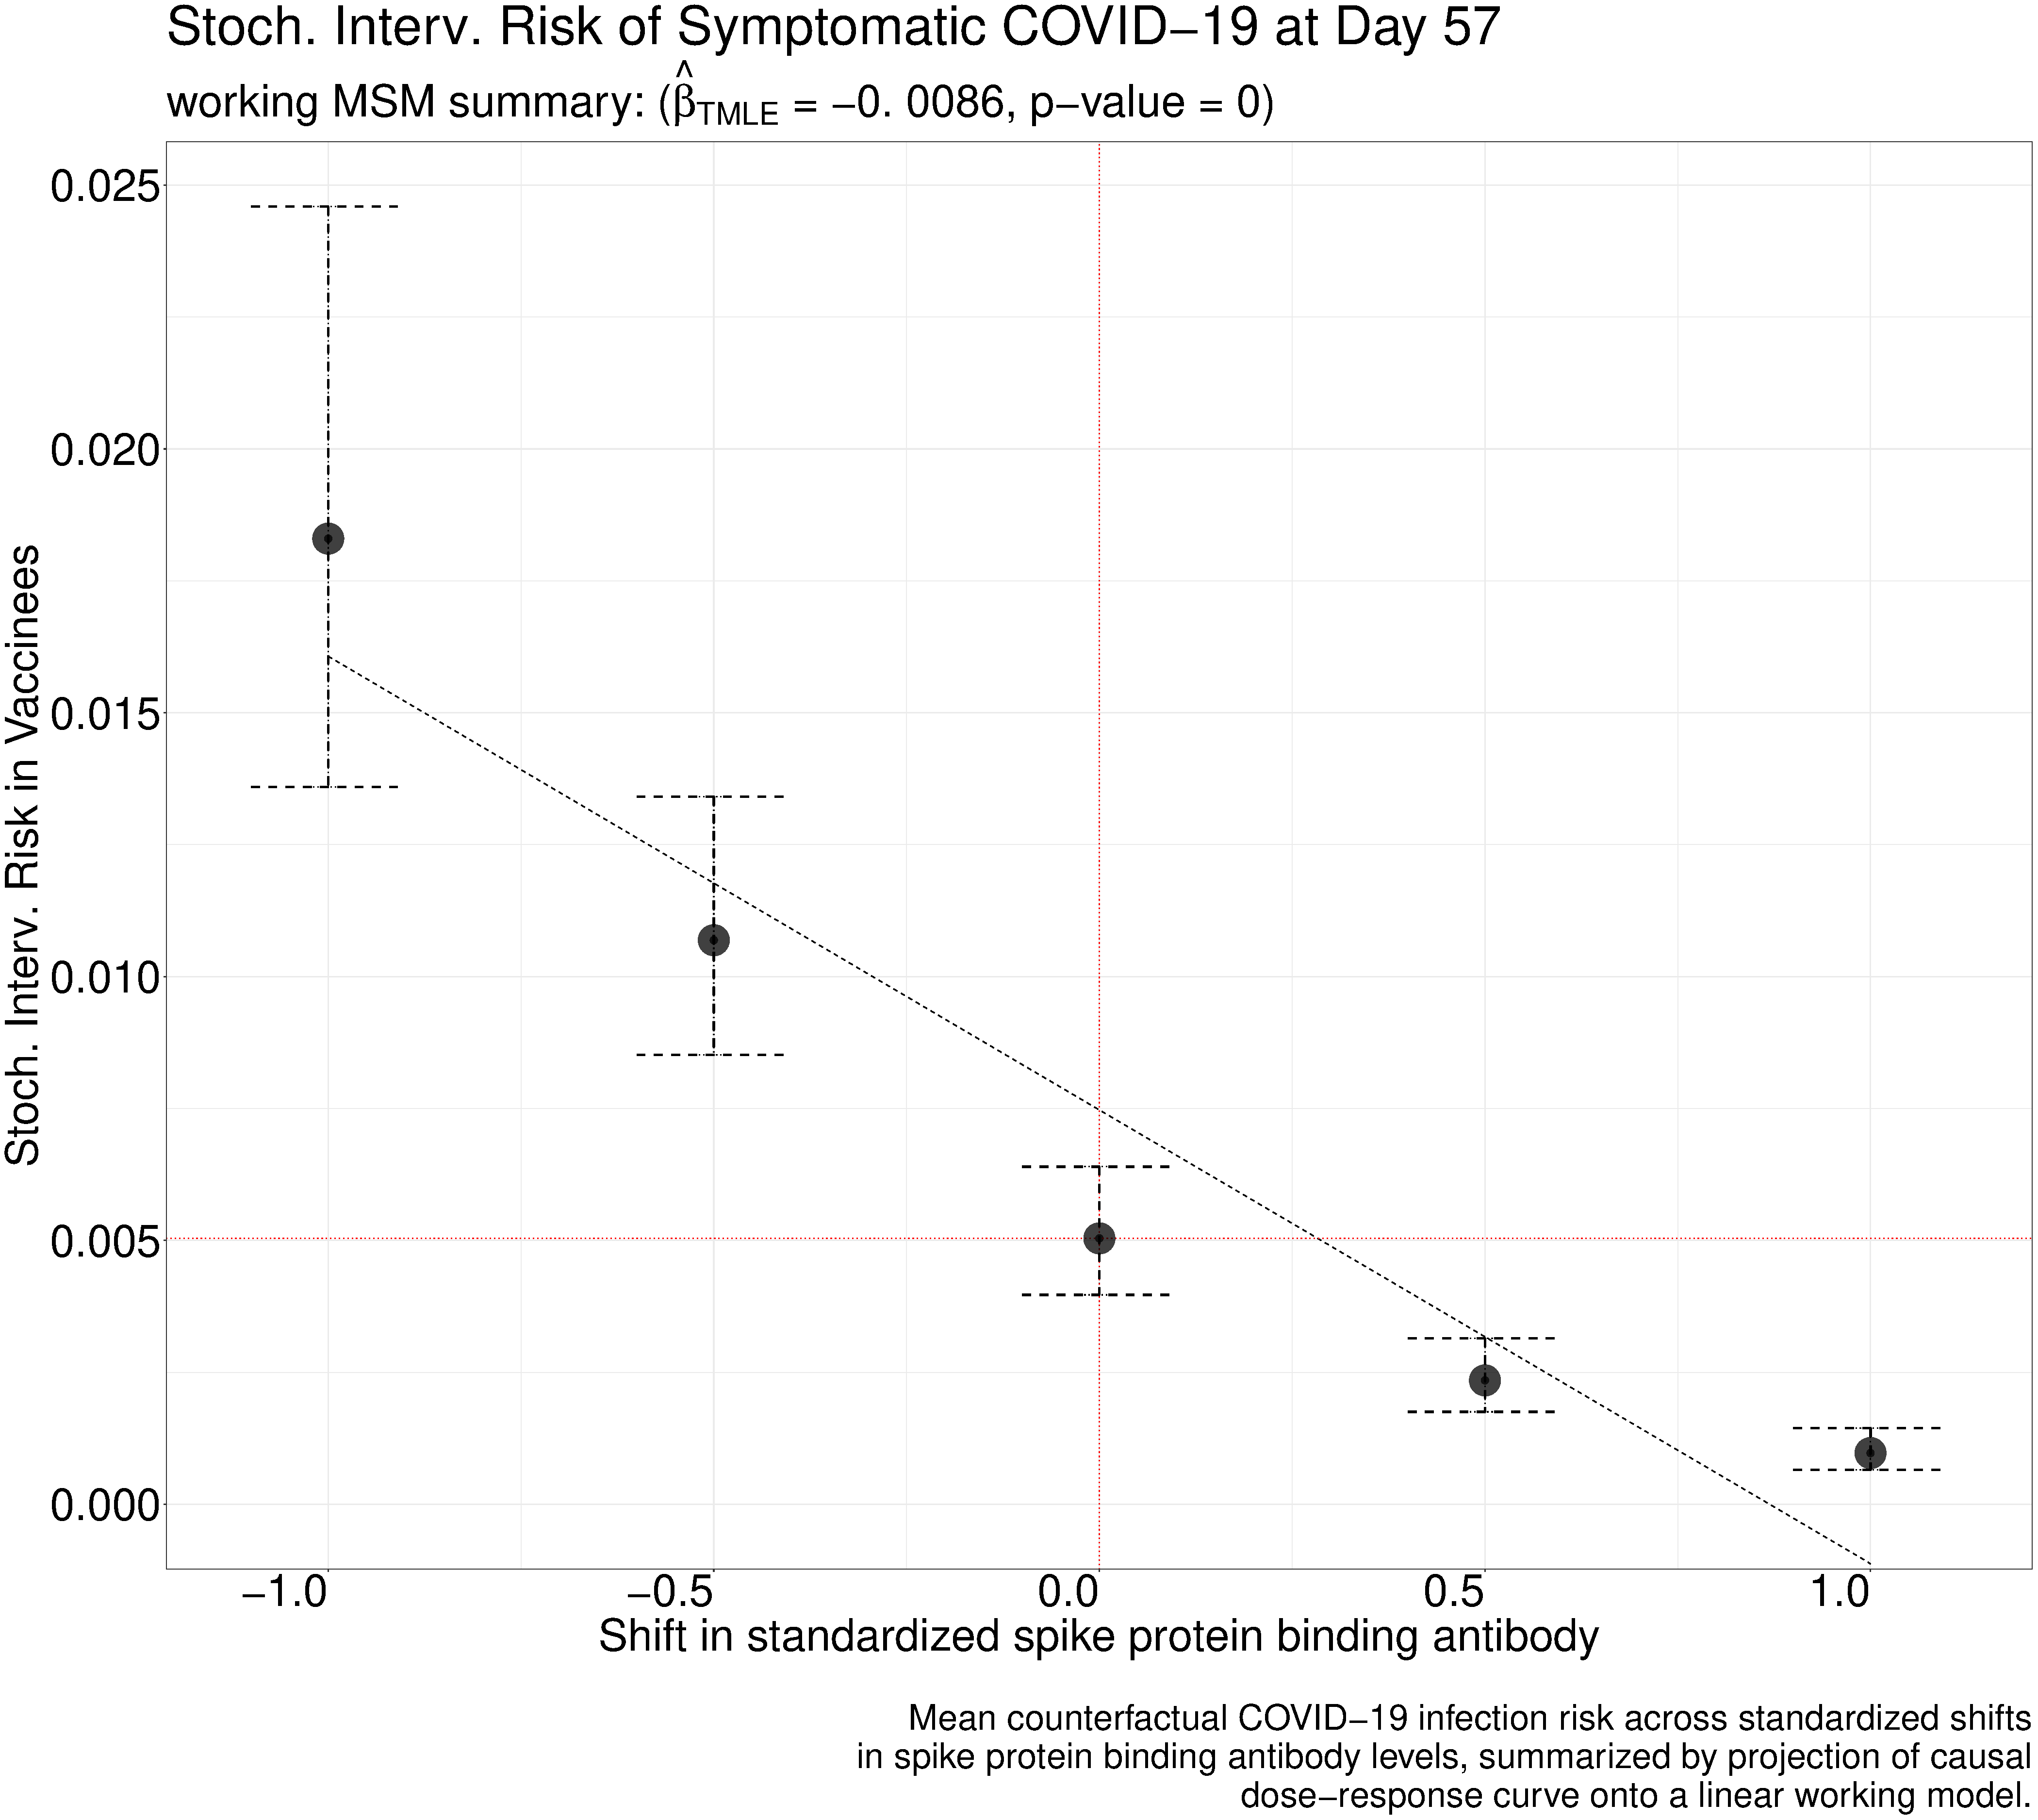
\includegraphics[width=0.975\linewidth,]{mcop_risk_Day57bindSpike}
  \caption{Stochastic interventional risk estimates, with confidence intervals,
  for the spike protein binding antibody at Day 57.}
  \label{fig:marker1-risk-day57}
\end{figure}

Estimation of the stochastic interventional risk for the spike protein antibody
across several values of $\delta$ reveals a monotonic decrease in risk with
increases in the activity of this immunologic marker. In particular, at $\delta
= 0$, for the vaccine administered in the current efficacy trial, the estimated
risk of symptomatic COVID-19 infection at Day 57 is 0.5\%. For positive values
of $\delta$, reflecting increased activity of the spike protein antibody, the
estimated risk of the adverse endpoint decreases towards zero. This suggests
that improvements to the dosage or formulation of the current vaccine may be
capable of improving its efficacy further still. Considering now negative values
of $\delta$, it appears that even moderate decreases in the modulation of this
antibody marker can significantly limit the efficacy of the vaccine against
infection. For example, with $\delta = -0.5$, the estimated risk doubles to
1.00\%; moreover, risk appears to grow sharply with further decreases in marker
activity. To summarize the trend in the change in estimated risk across the grid
in $\delta$, we note that projection onto a working marginal structural model
(MSM; as per Chapter~\ref{two}) yields a linear form with slope
$\hat{\beta}_{\text{TMLE}} = -0.0086$ and corresponding p-value of $p < 0.001$
for the hypothesis test of no trend (i.e., $H_0: \beta = 0$ and $H_1: \beta
\neq 0$).

\begin{figure}[H]
  \centering
  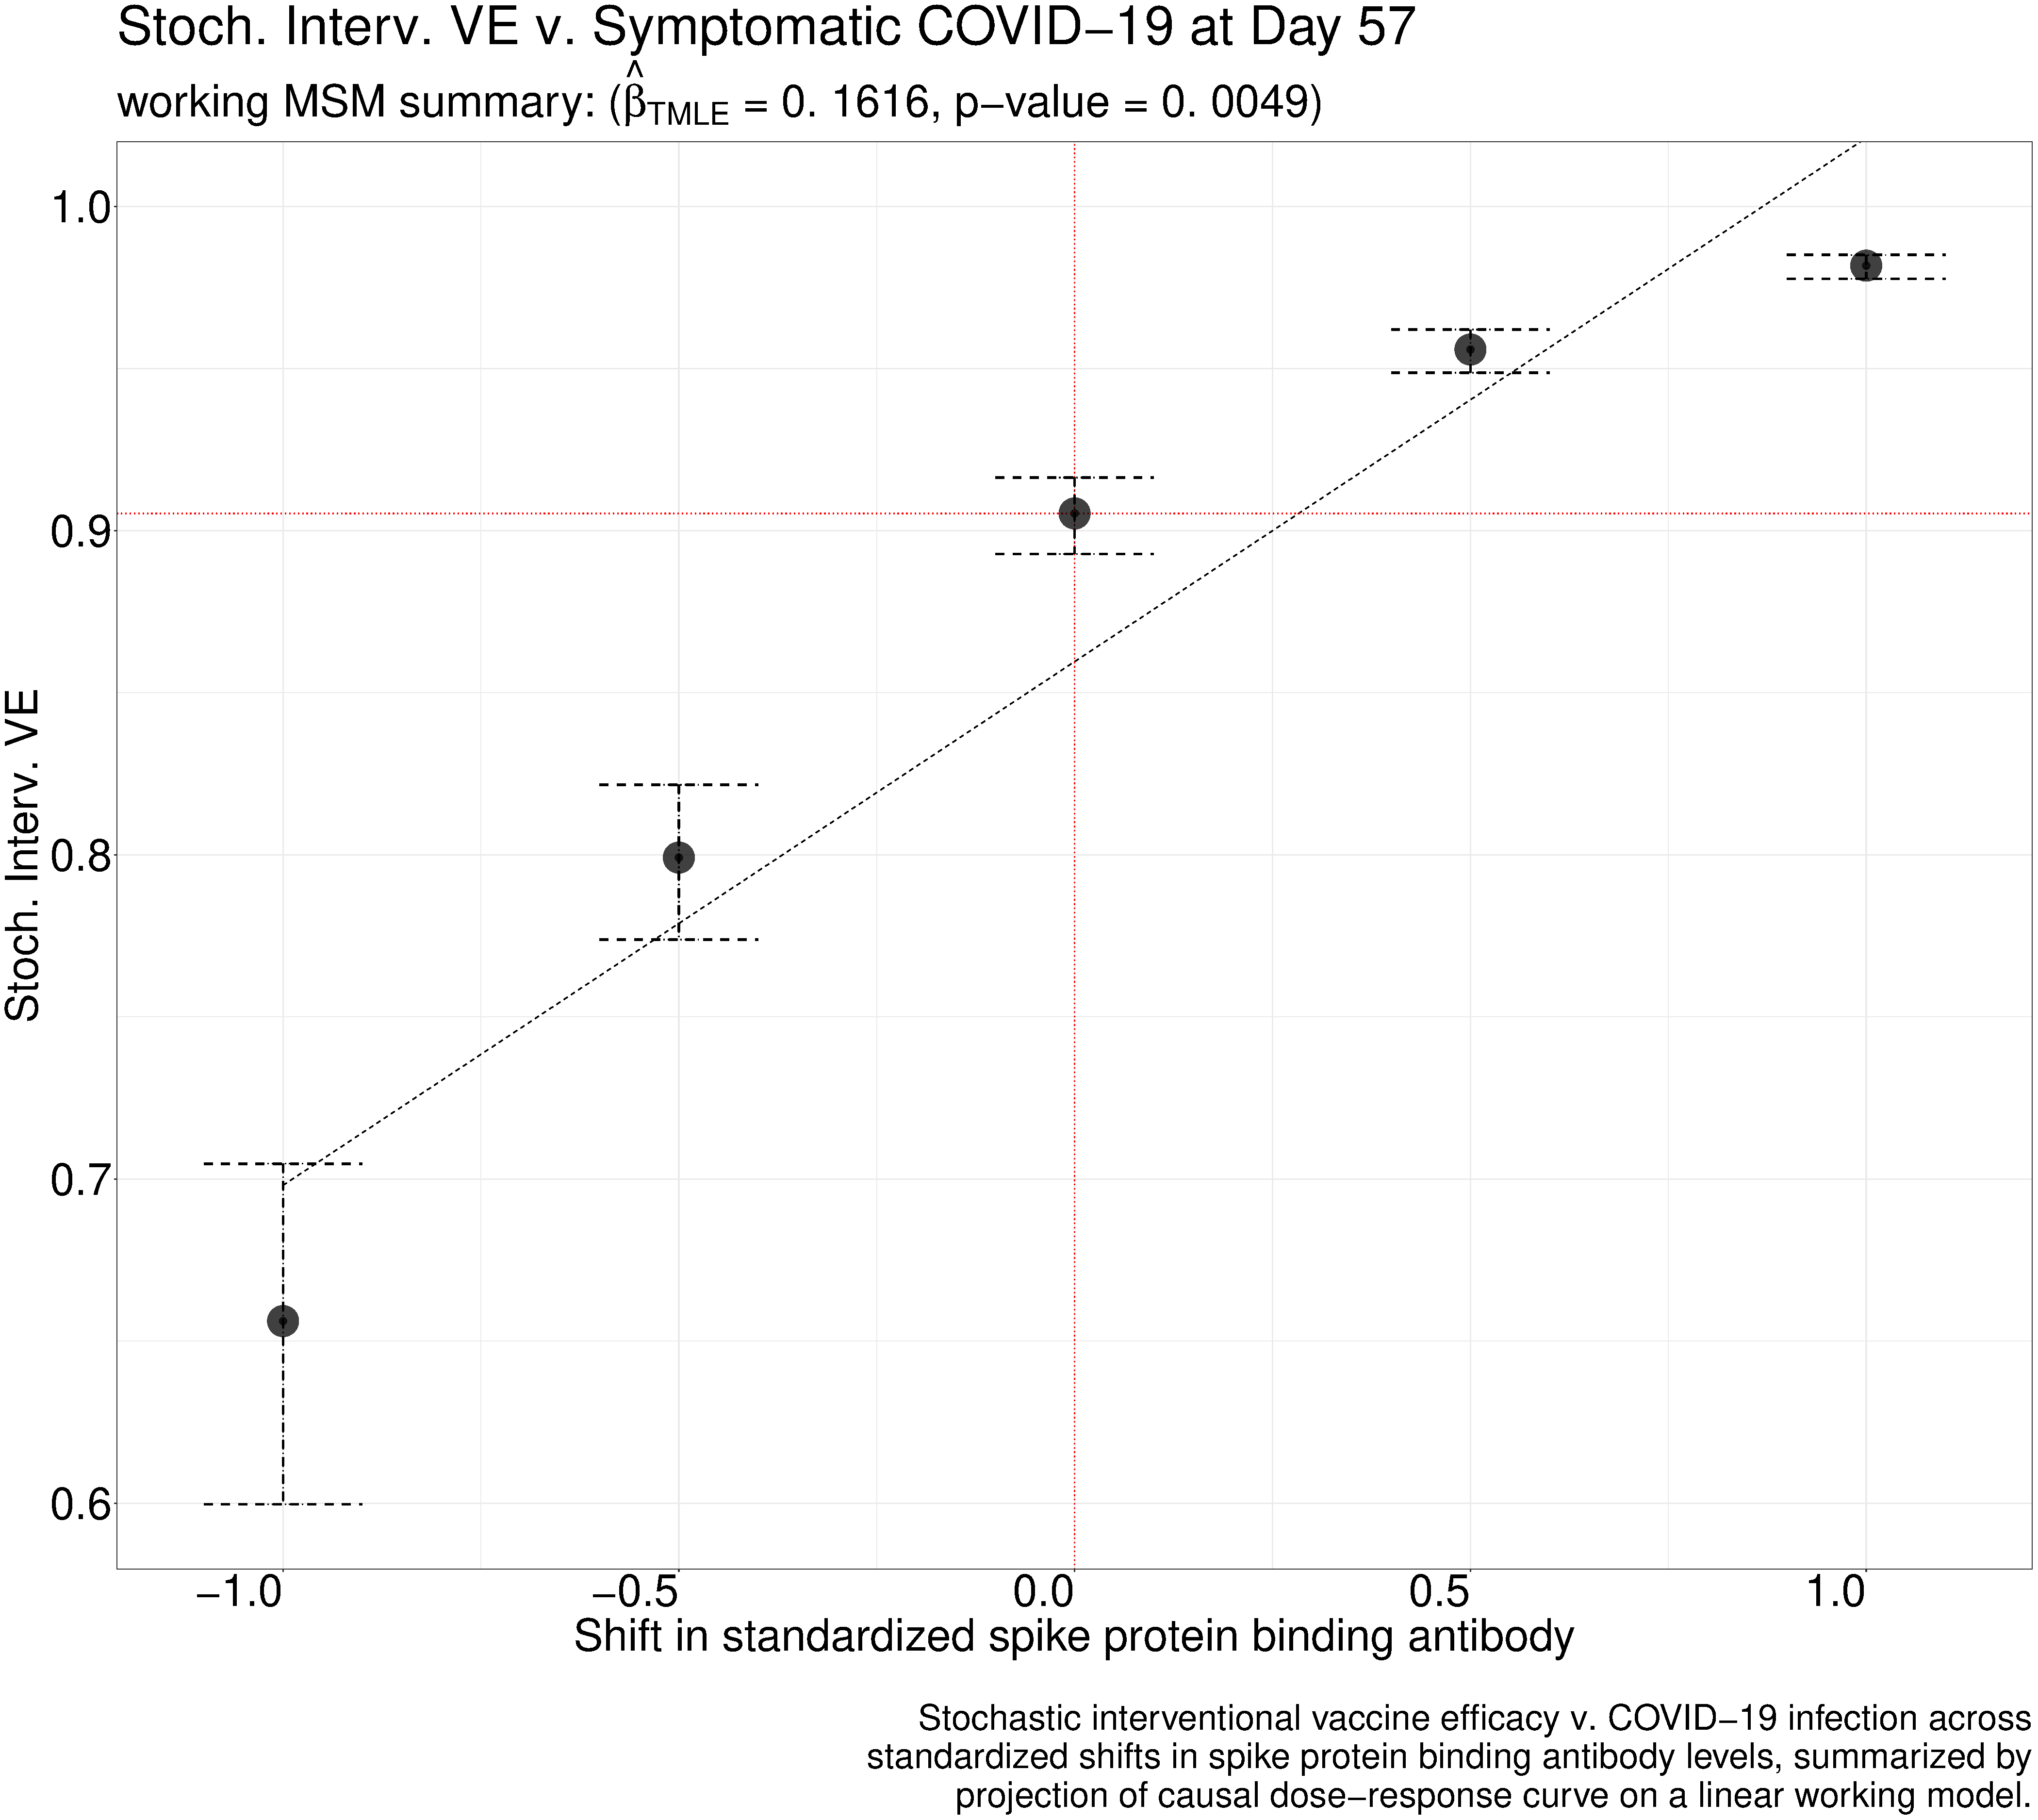
\includegraphics[width=0.975\linewidth,]{mcop_sve_Day57bindSpike}
  \caption{Stochastic interventional VE estimates, with confidence intervals,
    for the spike protein binding antibody at Day 57.}
  \label{fig:marker1-sve-day57}
\end{figure}

The evaluation of stochastic interventional VE is a process of re-scaling the
corresponding stochastic interventional risk estimates by the risk of infection
in the placebo arm of the trial, as per equation~\eqref{eqn:sve}. Accordingly,
the estimated VE provides information similar to that provided by the risk
estimates. In the case of the spike protein antibody, we find that the VE
produced by the administered vaccine (i.e., at $\delta = 0$) is just over 90\%.
What's more, upwards shifts of the activity of this marker have moderate impacts
on the estimated VE, with vaccine efficacy estimates of roughly 95\% and 97\%
for $\delta = 0.5$ and $\delta = 1$, respectively. While this analysis suggests
that reconstituting a future vaccine so as to specifically increase the activity
of the spike protein antibody may lead to very limited increases in protection,
the risk estimates at downwards shifts in its activity strongly suggest that all
vaccines ought to seek to module this marker at the level at which the current
vaccine does so. Specifically, a decrease of just a half standard unit (i.e.,
$\delta = -0.5$) leads to an estimated risk of 80\%, while a decrease of a full
standard unit ($\delta = -1$) yields a risk estimate of about 65\% --- 10\% and
25\% lower, respectively, than the risk estimate for the administered vaccine.
Examination of how VE estimates vary along the grid in $\delta$ reveals a sharp
increasing trend for the projection of the VE estimates onto a linear working
MSM. The slope parameter of the MSM is estimated to be
$\hat{\beta}_{\text{TMLE}} = 0.1616$ with a p-value of $p < 0.01$ for the
hypothesis test of no trend.

\begin{figure}[H]
  \centering
  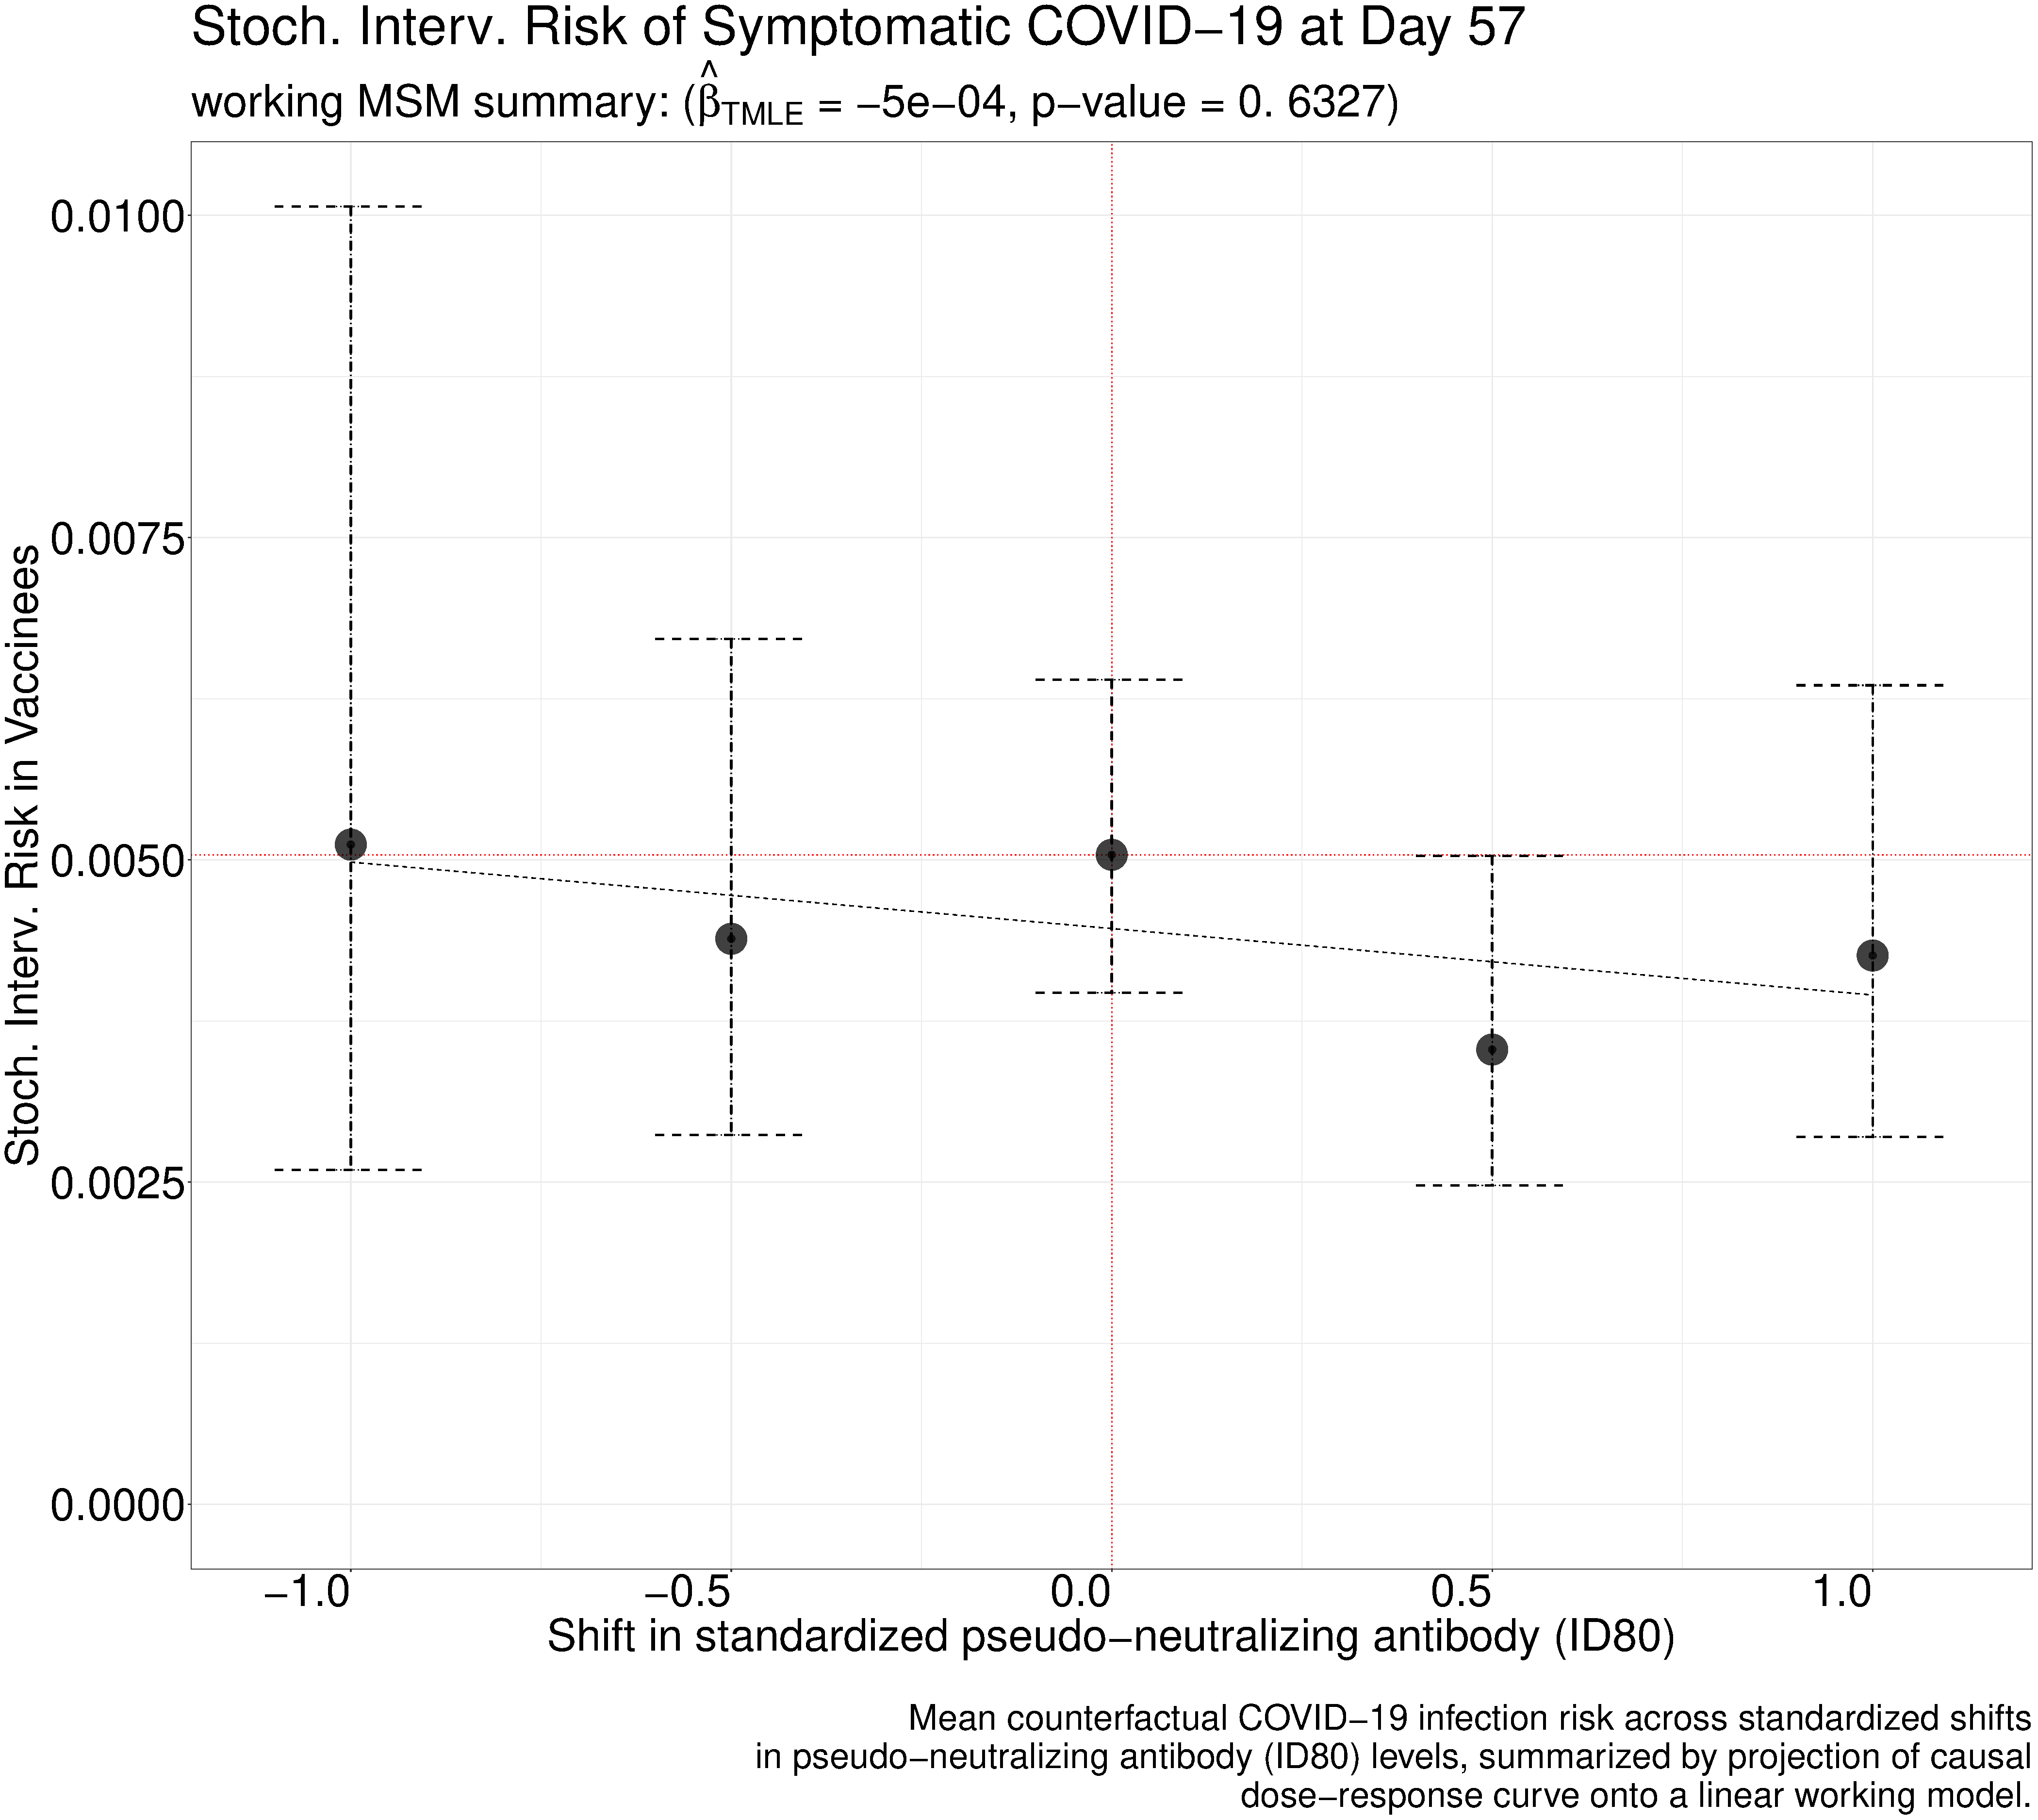
\includegraphics[width=0.975\linewidth,]{mcop_risk_Day57pseudoneutid80}
  \caption{Stochastic interventional risk estimates, with confidence intervals,
  for the pseudo-neutralizing antibody at Day 57.}
  \label{fig:marker4-risk-day57}
\end{figure}

Estimation of the stochastic interventional risk for the pseudo-neutralizing
antibody across the grid in $\delta$ reveals that the estimated risk is largely
insensitive to hypothetical changes in the marker activity. To start,
considering $\delta = 0$ (i.e., the activity of $S$ induced by the currently
administered vaccine), estimated risk of symptomatic COVID-19 infection at Day
57 is 0.5\%. The estimated stochastic interventional risk lies close to this
value for other values of $\delta$, suggesting that the pseudo-neutralizing
antibody may not be a suitable target for designing future vaccines to further
curb the risk of symptomatic COVID-19 infection.

\begin{figure}[H]
  \centering
  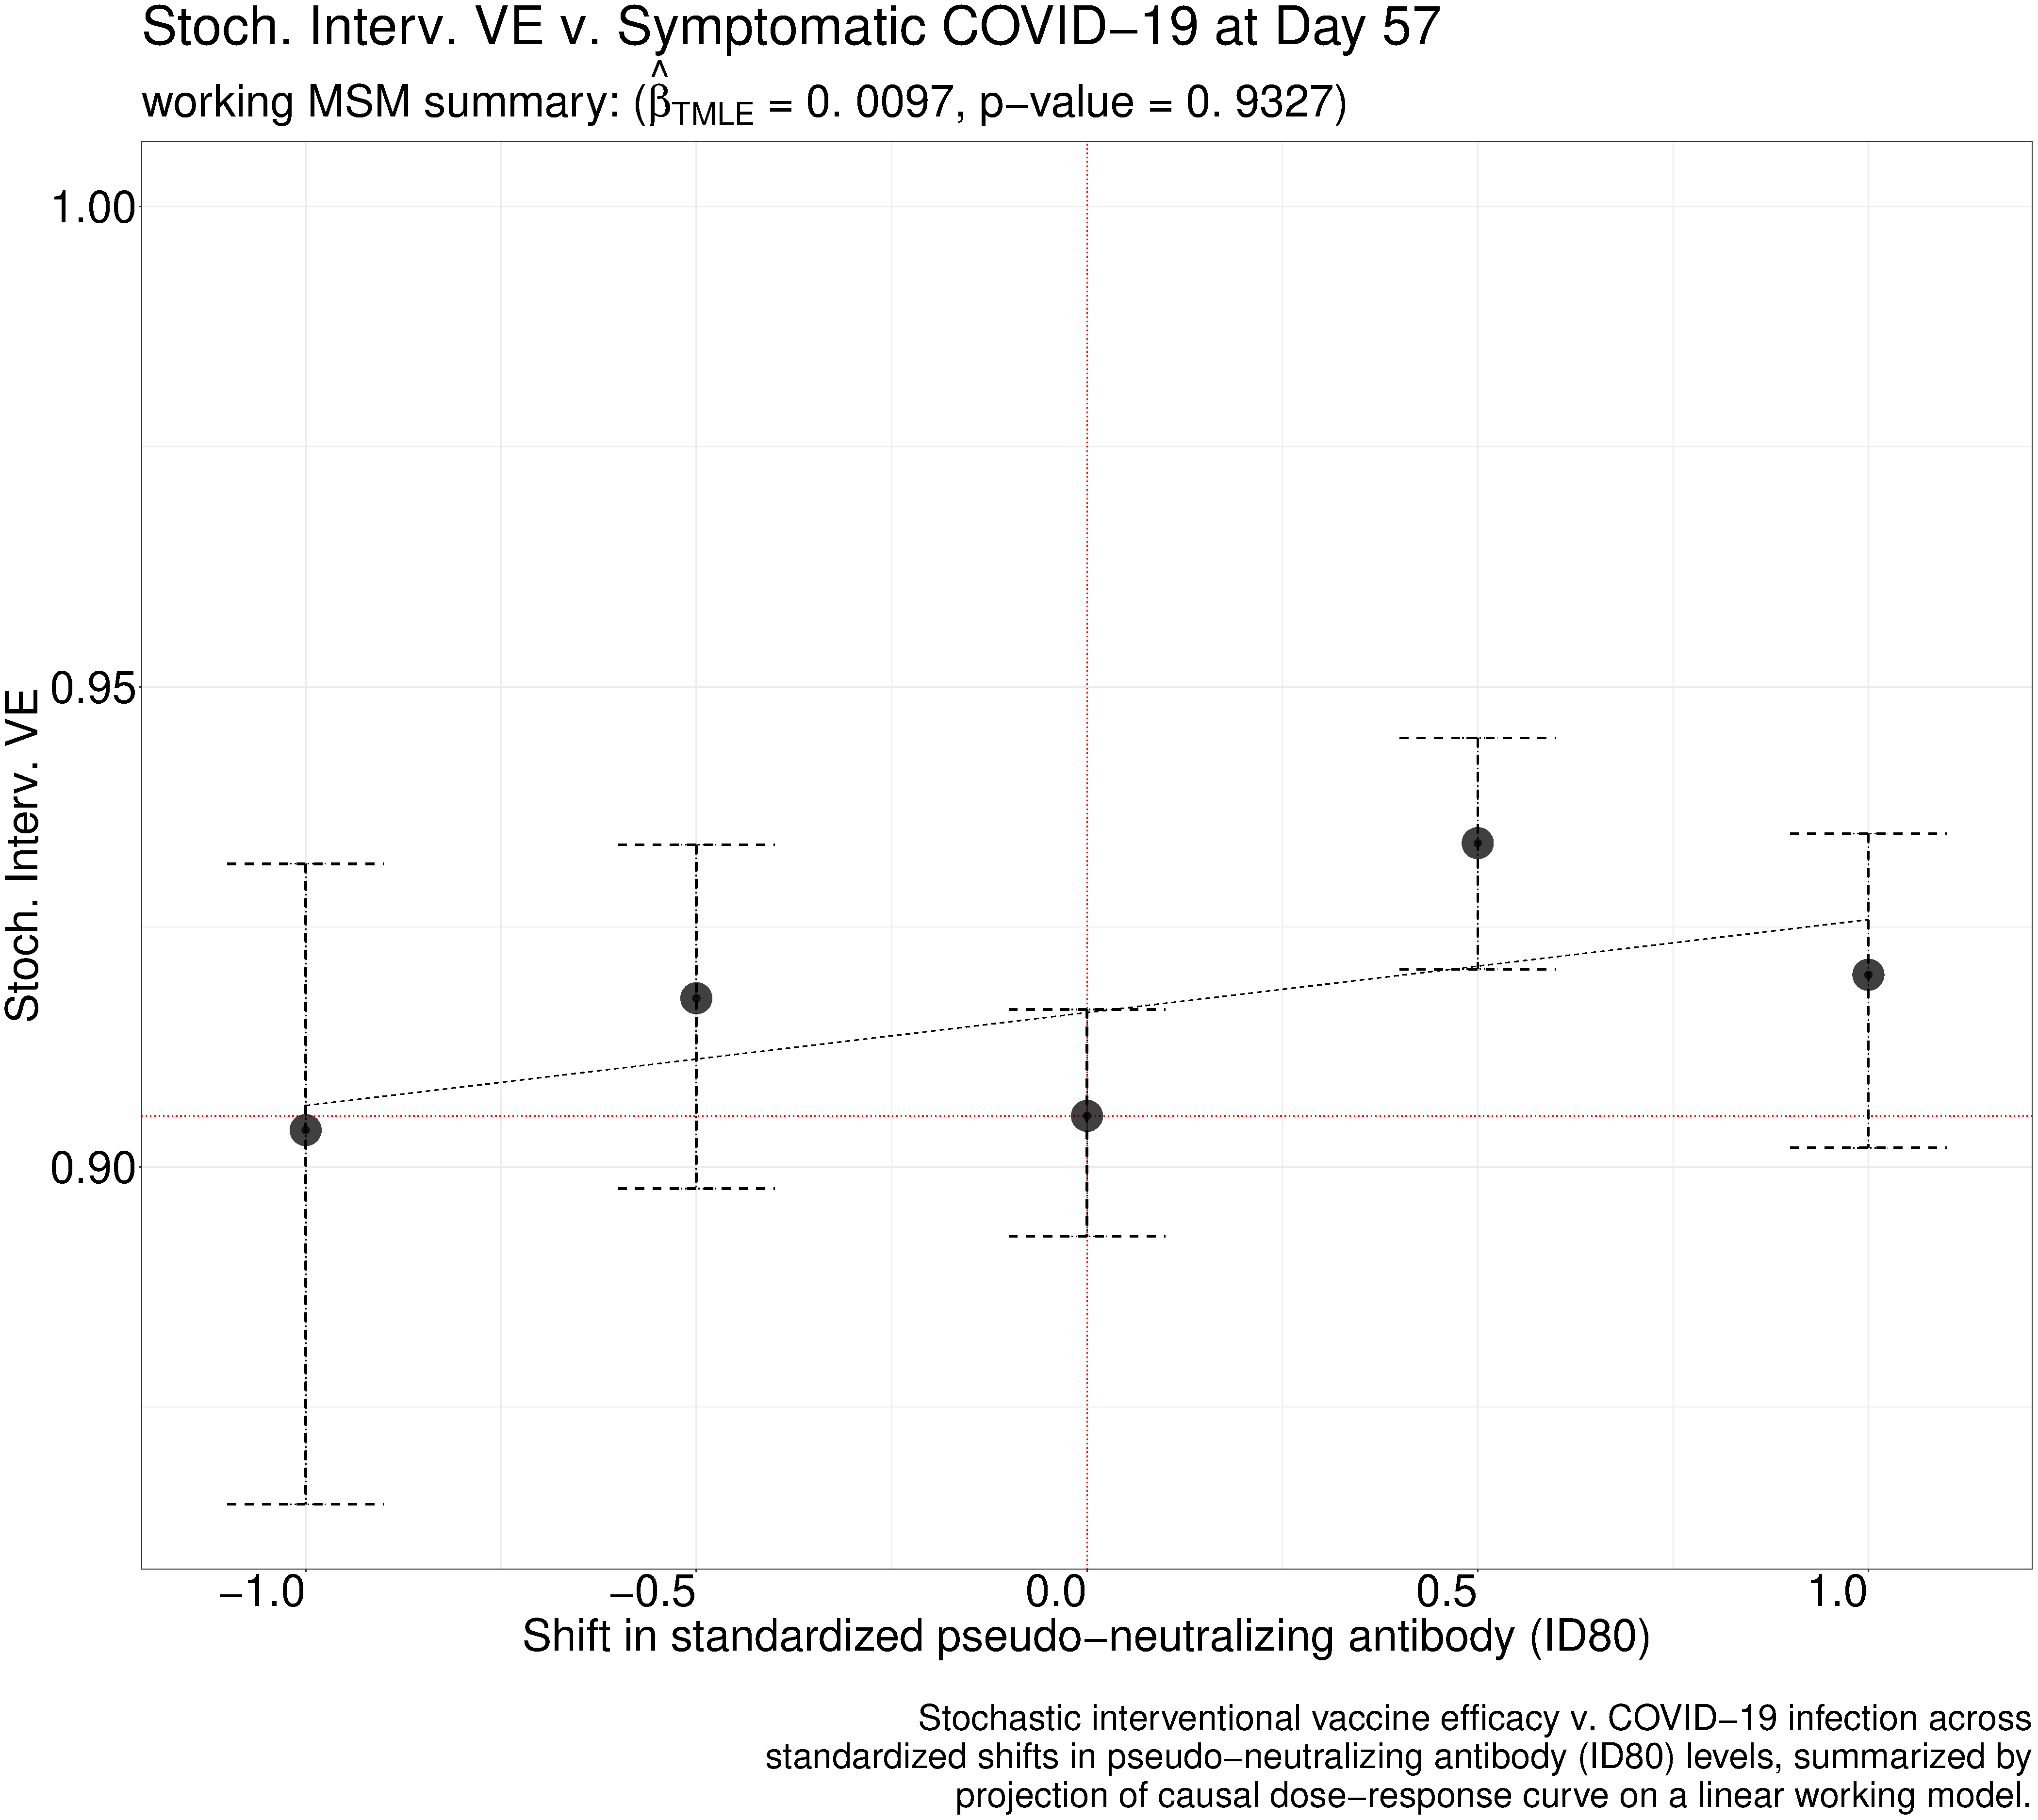
\includegraphics[width=0.975\linewidth,]{mcop_sve_Day57pseudoneutid80}
  \caption{Stochastic interventional VE estimates, with confidence intervals,
  for the pseudo-neutralizing antibody at Day 57.}
  \label{fig:marker4-sve-day57}
\end{figure}

Similarly to the estimates of the stochastic interventional risk for shifting of
the pseudo-neutralizing antibody, the stochastic VE estimates all lie within
roughly 3\% of the estimated VE at the null shift of $\delta = 0$. Examining the
VE estimate at that shift, we note an efficacy of roughly 90\%, with no sharp or
consistent changes in VE estimates at upwards or downwards shifts of the
activity of this marker. Consistent with the risk analyses, these VE estimates
suggest the pseudo-neutralizing antibody to be an unpromising candidate for
targeting by future vaccines.

\chapter{Stochastic Interventional Causal Mediation}\label{four}

Causal mediation analysis has historically been limited in two important ways:
(i) a focus has traditionally been placed on binary exposures and static
interventions, and (ii) direct and indirect effect decompositions have been
pursued that are only identifiable in the absence of intermediate confounders
affected by exposure. We present a theoretical study of an (in)direct effect
decomposition of the population intervention effect, defined by stochastic
interventions jointly applied to the exposure and mediators. In contrast to
existing proposals, our causal effects can be evaluated regardless of whether
a exposure is categorical or continuous and remain well-defined even in the
presence of intermediate confounders affected by exposure. Our (in)direct
effects are identifiable without a restrictive assumption on cross-world
counterfactual independencies, allowing for substantive conclusions drawn from
them to be validated in randomized controlled trials. Beyond the novel effects
introduced, we provide a careful study of nonparametric efficiency theory
relevant for the construction of flexible, multiply robust estimators of our
(in)direct effects, while avoiding undue restrictions induced by assuming
parametric models of nuisance parameter functionals. To complement our
nonparametric estimation strategy, we introduce inferential techniques for
constructing confidence intervals and hypothesis tests, and discuss open source
software, the \texttt{medshift} \texttt{R} package, implementing the proposed
methodology. Application of our (in)direct effects and their nonparametric
estimators is illustrated using data from a comparative effectiveness trial
examining the direct and indirect effects of pharmacological therapeutics on
relapse to opioid use disorder.

%%%%%%%%%%%%%%%%%%%%%%%%%%%%%%%%%%%%%%%%%%%%%%%%%%%%%%%%%%%%%%%%%%%%%%%%%%%%%%%
\section{Introduction}\label{sec:intro}
%%%%%%%%%%%%%%%%%%%%%%%%%%%%%%%%%%%%%%%%%%%%%%%%%%%%%%%%%%%%%%%%%%%%%%%%%%%%%%%

In myriad applications, one is often interested in the effect of an exposure on
an outcome only through a particular pathway between the two. Indeed, efforts in
defining and identifying such \textit{path-specific} effects have come to
constitute a rich history in not only philosophy but also in the sciences of
statistics, causal inference, epidemiology, economics, and psychology. In each
of these disciplines, as well as in many others among the biomedical and social
sciences, developing a mechanistic understanding of the complexities that admit
representations as path-specific effects remains a central goal; examples
include elucidating the biological mechanism by which a vaccine reduces
infection risk~\citep[e.g.,][]{corey2015immune, hejazi2020efficient}, assessing
the effect on preterm birth of maternal exposure to environmental
toxins~\citep[e.g.,][]{ferguson2017mediation}, and ascertaining the effect of
novel pharmacological therapies on substance abuse disorder relapse.

The latter serves as our motivating example as we consider how exposure to
a buprenorphine dose schedule characterized by successive increases toward
a maximum dose early in treatment (versus static dose) affects the risk of
relapse to opioid use disorder, both directly and indirectly through mediating
factors such as depression and pain. Developing a detailed mechanistic
understanding of the process by which such therapeutics modulate intermediary
states is necessarily a \textit{causal} question --- one central to designing
and successively improving upon available therapies in a manner targeted towards
the mitigation of the risk of substance abuse relapse. In comparative
effectiveness trials of promising opioid use disorder therapeutics, detailed
dissections of the complex neurological and psychiatric pathways involved in the
development of addiction disorders is of clinical
interest~\citep{lee2018comparative, rudolph2020explaining}. The ability to
define and evaluate causal effects along paths involving or avoiding mediating
neuropsychiatric sequela would facilitate drug efficacy assessments; moreover,
the ability to  refine scientific conclusions based on statistical evidence
through randomized controlled trials remains integral to furthering clinical
progress.

To carefully study complex mediation relationships, a wealth of techniques
rooted in statistical causal inference have been formulated. Path
analysis~\citep{wright1921correlation, wright1934method}, perhaps the earliest
example of such methodology, directly inspired the development of subsequent
techniques that leveraged parametric structural equation
models~\citep[e.g.,][]{goldberger1972structural, baron1986moderator} for
mediation analysis. More
recently, the advent of modern frameworks and formalisms for causal inference,
including nonparametric structural equation models, directed acyclic graphs,
and their underlying do-calculus~\citep{pearl1995causal, pearl2009causality},
provided the necessary foundational tools to express causal mechanisms without
reliance on more restrictive approaches tied to parametric modeling.

In tandem with the developments of~\citet{pearl2009causality}, similar
approaches spearheaded by~\citet{robins1986new}, \citet{spirtes2000causation},
\citet{dawid2000causal}, and~\cite{richardson2013single} allowed nonparametric
formulations of mediation analysis and uncovered significant limitations of the
earlier efforts focused on structural equation models~\citep{pearl1998graphs,
imai2010general}. Recent applications of modern causal models have illustrated
the failings of popular parametric modeling
strategies~\citep[i.e.,][]{baron1986moderator}, in the presence of intermediate
confounders of the mediator-outcome relationship~\citep{cole2002fallibility}.
Consequently, the usually implausible assumptions that underlie such restrictive
structural equation models make these approaches of limited applicability for
the examination of complex phenomena in the biomedical, health, and social
sciences.

Modern approaches to causal inference have allowed for significant advances over
the methodology of traditional mediation analysis, overcoming the significant
restrictions imposed by the use of parametric structural equation modeling. For
example,~\citet{robins1992identifiability} and~\citet{pearl2001direct}, using
distinct frameworks, provided equivalent nonparametric decompositions of the
average treatment effect (for binary exposures) into the \textit{natural}
direct and indirect effects, which quantify all effects of the treatment on the
outcome through paths avoiding the mediator and all paths involving the
mediator, respectively. Such advances were not without their limitations,
however. A key assumption of the nonparametric decomposition of the average
treatment effect is the requirement of \textit{cross-world} counterfactual
independencies (i.e., the condition that counterfactuals indexed by distinct
intervention assignments be independent). Unfortunately, such an assumption
limits the scientific relevance of the natural (in)direct effects by making them
unidentifiable in randomized trials, directly implying that corresponding
scientific claims cannot be falsified through
experimentation~\citep{popper1934logic, dawid2000causal, robins2010alternative}.
Importantly, such cross-world independencies are also unsatisfied in the
presence of intermediate confounders affected by
treatment~\citep{avin2005identifiability, tchetgen2014identification}. As such
confounders are often present in practice, the natural (in)direct effects are
of limited applicability.

A related thread of the literature has considered stochastic interventions,
which generalize many intervention classes. For example, within this framework,
static interventions result in post-intervention exposures that have degenerate
distributions. \citet{stock1989nonparametric} first considered the estimation of
the total effects of stochastic interventions, while many
others~\citep[e.g.,][]{robins2004effects, didelez2006direct,
tian2008identifying, pearl2009myth, stitelman2010impact, haneuse2013estimation,
diaz2013assessing, dudik2014doubly, young2014identification} provided careful
studies that expanded the underlying theory of stochastic interventions and
demonstrated their numerous applications. Uniquely, stochastic interventions can
be applied to define causal effects of continuous-valued exposures, with an
interpretation echoing that of regression adjustment. For
example,~\citet{diaz2012population} and~\citet{haneuse2013estimation} described
modified treatment policies, which assign post-intervention counterfactuals
based on the natural value of the exposure; their methods were demonstrated in
the context of increasing leisure physical activity in the elderly and reducing
surgical time for non-small-cell lung cancer operations. Stochastic
interventions have also successfully been applied to binary exposures:
\citet{kennedy2019nonparametric} proposed incremental propensity score
interventions and demonstrated their use in longitudinal studies in order to
circumvent identifiability and estimation issues arising from positivity
violations.

Contemporaneously,~\citet{diaz2020causal} proposed a decomposition of the total
effect of stochastic interventions into the population intervention (in)direct
effects, which are endowed with interpretations analogous to that of the natural
(in)direct effects. Prior related attempts at the
same~\citep[e.g.,][]{vansteelandt2012imputation} introduced parametric modeling
assumptions to lessen reliance on the assumption of cross-world counterfactual
independencies, introducing flexibility at the cost of bias and restrictive
assumptions on post-intervention distributions. In a similar vein, the
stochastic (in)direct effects of~\citet{diaz2020causal} do not require
cross-world counterfactual independencies but succeed in accommodating
nonparametric estimation strategies. Consequently, these population intervention
(in)direct effects may be estimated without restrictive assumptions and yield
scientific results that can be tested through randomization of both the
exposure and mediator. Despite these advances, the results
of~\citet{diaz2020causal} suffer a serious shortcoming --- that is, these
effects lack identifiability in the presence of intermediate confounders, which
affect both mediators and outcome and are themselves affected by the exposure.
This incompatibility with intermediate confounding motivated the development of
a new and promising family of \textit{interventional} (in)direct
effects~\citep{didelez2006direct, vanderweele2014effect, lok2016defining,
vansteelandt2017interventional, zheng2017longitudinal, rudolph2017robust,
lok2019causal, nguyen2020clarifying}, which utilize joint static and stochastic
interventions (applied to the exposure and mediators, respectively) to retain
identifiability under such confounding. Until recently, nonparametric effect
decompositions and efficiency theory were unavailable for this class of effects,
though efforts by \citet{diaz2020nonparametric} and
\citet{benkeser2020nonparametric} have sought to provide some remedy. While
resolving the issues arising from requiring cross-world counterfactual
independencies, these interventional (in)direct effects are limited by their
lack of applicability beyond binary exposures.

In the present work, we outline a general framework encompassing many prior
causal mediation analysis approaches, including the natural (in)direct effects,
their interventional effect counterparts, and the stochastic (in)direct effects.
Building upon the foundations laid by \citet{diaz2020causal}, the introduced
class of mediation effects originate from combining the novel lines of inquiry
established in the distinct literatures on stochastic interventions and the
interventional effects; accordingly, we denote these \textit{stochastic
interventional (in)direct effects}. Our proposed class of effects are the first
to simultaneously avoid the requirement of cross-world counterfactual
independencies; leverage stochastic interventions to be applicable to binary,
categorical, and continuous-valued exposures; and remain identifiable despite
intermediate confounding. As such, our contributions apply to a broader class of
exposures than the interventional effects~\citep[e.g.,][]{diaz2020nonparametric,
benkeser2020nonparametric} while generalizing stochastic (in)direct
effects~\citep[e.g.,][]{diaz2020causal} to accommodate the presence of
intermediate confounders. While our robust and flexible causal mediation
analysis framework subsumes prior classes of effect definitions, this is far
from enough for the successful application of our proposed (in)direct effects.
To this end, we develop novel efficiency theory and efficient nonparametric
estimators of this broad new class of causal mediation parameters, within the
frameworks of one-step~\citep{pfanzagl1985contributions, bickel1993efficient}
and targeted minimum loss estimation~\citep{vdl2006targeted, vdl2011targeted,
vdl2018targeted}. These flexible estimators have desirable asymptotic properties
even when nuisance parameter functionals are estimated via machine learning;
moreover, they are endowed with a form of multiple robustness producing
consistent point estimates under several configurations of nuisance parameter
misspecification. Lastly, we provide implementations of our methodological
advances in our free and open source
\texttt{medshift}~\citep{hejazi2020medshift} package, for the \texttt{R}
language and environment for statistical computing~\citep{R}.

%%%%%%%%%%%%%%%%%%%%%%%%%%%%%%%%%%%%%%%%%%%%%%%%%%%%%%%%%%%%%%%%%%%%%%%%%%%%%%%
\section{Mediation Analysis for the Population Intervention
  Effect}\label{sec:backg}
%%%%%%%%%%%%%%%%%%%%%%%%%%%%%%%%%%%%%%%%%%%%%%%%%%%%%%%%%%%%%%%%%%%%%%%%%%%%%%%
Let $A$ denote a continuous or categorical exposure variable, $Y$ denote
a continuous or binary outcome, $Z$ denote mediator(s), $W$ denote
a vector of observed pre-exposure covariates, and $L$ denote an
intermediate (mediator-outcome) confounder affected by exposure. We formalize
the causal inference problem via the nonparametric structural
equation model (NPSEM):
\begin{align}\label{eq:npsem}
  W &= f_W(U_W); A = f_A(W, U_A); L = f_L(A, W, U_L);\\ \nonumber
  Z &= f_Z(L, A, W, U_Z); Y = f_Y(Z, L, A, W, U_Y).
\end{align}
In the NPSEM (\ref{eq:npsem}), $U=(U_W,U_A,U_L,U_Z,U_Y)$ is a vector of
exogenous factors, and the functions $f$ are assumed deterministic but unknown.
This mechanistic model is assumed to generate the observed data $O$; it encodes
several fundamental assumptions. First, an implicit temporal ordering $W
\rightarrow A \rightarrow L \rightarrow Z \rightarrow Y$ is assumed. Second,
each variable (i.e., $\{W, A, L, Z, Y\}$) is assumed to be generated from the
corresponding deterministic function of the observed variables that precede it
temporally, plus an exogenous variable denoted by $U$. Each exogenous variable
is assumed to contain all unobserved causes of the corresponding observed
variable. For a random variable $X$, let $X_a$ denote the counterfactual outcome
observed in a hypothetical world in which $\P(A=a)=1$. For example, we have
$L_a = f_L(a, W,U_L)$, $Z_a=f_Z(L_a, a, W,U_Z)$, and $Y_a=f_Y(Z_a, L_a, a, W,
U_Y)$. Likewise, we let $Y_{a,z} = f_Y(z, L_a, a, W,U_Y)$ denote the value of
the outcome in a hypothetical world where $\P(A = a, Z = z)=1$.
Figure~\ref{fig:dag} represents model (\ref{eq:npsem}) in terms of a directed
acyclic graph (DAG).
\begin{figure}[!htb]
  \centering
  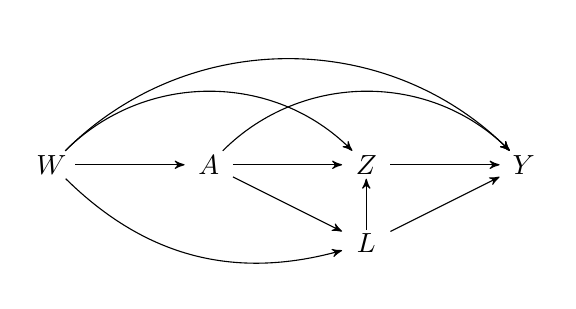
\begin{tikzpicture}
    \Vertex{0, -1}{L}
    \Vertex{-4, 0}{W}
    \Vertex{0, 0}{Z}
    \Vertex{-2, 0}{A}
    \Vertex{2, 0}{Y}
    \ArrowR{W}{L}{black}
    \Arrow{L}{Z}{black}
    \Arrow{W}{A}{black}
    \Arrow{A}{Z}{black}
    \Arrow{Z}{Y}{black}
    \Arrow{A}{L}{black}
    \Arrow{L}{Y}{black}
    \ArrowL{W}{Y}{black}
    \ArrowL{A}{Y}{black}
    \ArrowL{W}{Z}{black}
  \end{tikzpicture}
  \caption{Directed Acyclic Graph of NPSEM (\ref{eq:npsem}).}
  \label{fig:dag}
\end{figure}

Letting $O = (W, A, Z, L, Y)$ represent a random variable with distribution
$\P$, we denote by $O_1, \ldots, O_n$ a sample of $n$ i.i.d.~observations of
$O$. We let $\P f = \int f(o)\dd \P(o)$ for a given function $f(o)$. We use
$\P_c$ to denote the joint distribution of $(O,U)$, and let $\E$ and $\E_c$
denote corresponding expectation operators. We use $\Pn$ to denote the empirical
distribution of $O_1, \ldots, O_n$, and assume $\P \in \M$, where $\M$ is the
nonparametric statistical model defined as all continuous densities on $O$ with
respect to a dominating measure $\nu$. Let $\p$ denote the corresponding
probability density function. We use $\g(a \mid w)$ and $\e(a \mid z, w)$ to
denote the probability density function or the probability mass function of $A$
conditional on $W = w$ and $(Z, W)$, respectively; $\m(z,l,a,w)$ to denote the
outcome regression function $\E(Y \mid Z = z,L=l,A = a,W = w)$. Let
$\g(\cdot\mid w)$ and $\e(\cdot\mid z,w)$ be dominated by a measure $\kappa(a)$
(e.g., the counting measure for binary $A$ and the Lebesgue measure for
continuous $A$). % We also use $\q(z \mid a,w)$ and $\r(z \mid w)$ to
% denote the corresponding conditional densities of $Z$.
We will use the parameterizations
\begin{equation}
  \frac{\p(z\mid w)}{\p(z\mid a, w)} = \frac{\g(a\mid w)}{\e(a\mid z,w)};
    \quad\quad \frac{\p(z\mid a,w)}{\p(z\mid l,a,w)}=
    \frac{\p(l\mid a,w)}{\p(l\mid z,a,w)}\label{eq:parameterize}
\end{equation}
in constructing our estimators, as such parameterizations allow for estimation
and integration with respect to multivariate conditional densities on the
mediator $Z$ to be avoided. We use $\cal W, \cal A, \cal Z$, $\cal L$, and
$\cal Y$ to denote the support of the corresponding random variables.

Causal effects are defined in terms of hypothetical interventions on the
NPSEM~\eqref{eq:npsem}. In particular, consider an intervention in which the
structural equation corresponding to $A$ is removed, with the treatment drawn
instead from a user-specified distribution $g_\delta(a \mid w)$, which may
itself depend on the natural exposure distribution and a user-specified
parameter $\delta$. Going forward, we let $A_\delta$ denote a draw from
$g_\delta(a \mid w)$. Alternatively, such modifications can occasionally be
described in terms of an intervention in which the structural equation
corresponding to $A$ is removed and the treatment is set equal to a hypothetical
regime $d(A, W)$. Regime $d$ depends on the treatment level $A$ that would be
assigned in the absence of the regime as well as on $W$. The latter intervention
has been referred to as depending on the \textit{natural value of treatment}, or
as a \textit{modified treatment policy}~\citep{haneuse2013estimation}. For such
interventions, \citet{haneuse2013estimation} introduced the assumption of
\textit{piecewise smooth invertibility}, which ensures that the change of
variable formula can be used when computing integrals over $\cal A$:
\begin{assumptioniden}[Piecewise smooth invertibility]\label{ass:inv}
  For each $w \in \cal W$, assume that the interval
  ${\cal I}(w) = (l(w,), u(w))$ may be partitioned into subintervals
  ${\cal I}_{\delta,j}(w):j = 1, \ldots, J(w)$ such that $d(a, w)$ is equal to
  some $d_j(a, w)$ in ${\cal I}_{\delta,j}(w)$ and $d_j(\cdot,w)$ has inverse
  function $h_j(\cdot, w)$ with derivative $h_j'(\cdot, w)$.
\end{assumptioniden}
Assumption~\ref{ass:inv} can be used to show that the intervention drawing
$A_{\delta}$ from the post-intervention distribution $\g_\delta(a \mid w)$ can
be interpreted on the individual level. \citet{young2014identification} provide
a discussion comparing and contrasting the interpretation and identification of
these two interventions. Such stochastic interventions can be used to define the
\textit{population intervention effect (PIE)} of $A$ on $Y$. To illustrate,
consider continuous-valued $A$ and assume the distribution of $A$ conditional on
$W = w$ is supported in the interval $(l(w), u(w))$. Then, one may define
\begin{equation}\label{eq:defdshift}
  d(a, w) =
  \begin{cases}
    a - \delta & \text{if } a > l(w) + \delta \\
    a & \text{if } a \leq l(w) + \delta,
  \end{cases}
\end{equation}
where $0 < \delta < u(w)$ is an arbitrary prespecified value. We
can alternatively define a tilted intervention distribution as
\begin{equation}\label{eq:tilt}
  \g_\delta(a \mid w) = \frac{\exp(\delta a) \g(a \mid w)}
  {\int \exp(\delta a) \g(a\mid w)\dd\kappa(a)},
\end{equation}
for $\delta \in \mathbb R$. % As a simple example, consider a random
% variable $A \mid W = w \sim N\{\mu(w), \sigma^2(w)\}$. Under the
% intervention, $A$ is distributed as
% $N\{\mu(w) + \delta \sigma^2(w), \sigma^2(w)\}$.
\citet{kennedy2019nonparametric} proposed a form of exponential tilting
(\ref{eq:tilt}) under the parameterization $\delta' = \exp(\delta)$, appropriate
for incremental interventions on the propensity score for binary $A$.
\citet{diaz2020causal} provide a careful study of the
interventions~\ref{eq:defdshift} and~\ref{eq:tilt} in the context of mediation,
introducing novel (in)direct effects and corresponding efficiency theory;
however, their contributions assume the absence of intermediate confounding.

%For binary $A$,~\cite{kennedy2019nonparametric} proposed evaluating the total
%effect of a binary treatment $A$ in terms of incremental propensity score
%interventions that replace the propensity score $g(1 \mid w)$ with a shifted
%variant constructed from multiplying the odds of treatment by a user-specified
%parameter $\delta'$. In particular, the post-intervention propensity score is
%\begin{equation}\label{eq:incremental}
  %\g_{\delta'}(1 \mid w) = \frac{\delta' \g(1 \mid w)}{\delta'
  %\g(1 \mid w) + 1 - \g(1\mid w)},
%\end{equation}
%for $0 < \delta' < \infty$.

%As this characterization will be useful for studying the
%properties of the parameter and estimators we propose, we review it briefly in
%the sequel.
%\begin{assumptioniden}[Piecewise smooth invertibility]\label{ass:inv}
  %For each $w \in \cal W$, assume that the interval
  %${\cal I}(w) = (l(w,), u(w))$ may be partitioned into subintervals
  %${\cal I}_{\delta,j}(w):j = 1, \ldots, J(w)$ such that $d(a, w)$ is equal to
  %some $d_j(a, w)$ in ${\cal I}_{\delta,j}(w)$ and $d_j(\cdot,w)$ has inverse
  %function $h_j(\cdot, w)$ with derivative $h_j'(\cdot, w)$.
%\end{assumptioniden}
%Under this assumption, the stochastic intervention associated with any modified
%treatment policy $d(A,W)$ may be recovered through
%\begin{equation}\label{eq:gdelta}
  %\g_\delta(a \mid w) =
  %\sum_{j=1}^{J(w)} I_{\delta, j} \{h_j(a, w), w\} \g\{h_j(a, w)\mid w\}
  %h_j'(a,w),
%\end{equation}
%where $I_{\delta, j} \{u, w\} = 1$ if $u \in {\cal I}_{\delta, j}(w)$ and
%$I_{\delta, j}\{u, w\} = 0$ otherwise. The density associated with the
%intervention (\ref{eq:defdshift}) becomes $\g_\delta(a\mid w) = \g(a\mid w)
%\one\{l(w)\leq a \leq l(w) + \delta\} + \g(a+\delta\mid w) \one\{l(w)\leq a
%\leq u(w) - \delta\}$. Therefore, the intervention may also be represented as
%a change in which the structural equation $f_A$ is removed from the NPSEM, with
%$A$ instead being drawn from the post-intervention distribution $\g_\delta(a
%\mid w)$. Such stochastic interventions can be used to define the
%\textit{population intervention effect (PIE)} of $A$ on $Y$.

\subsection{Stochastic Mediation Effects}

\citet{diaz2020causal} defined the (in)direct effect of $A$ on $Y$ in
terms of a decomposition of the total effect of a stochastic
intervention. In particular, the total effect $\E(Y - Y_{A_\delta})$ may be
decomposed as the sum of the population intervention direct and indirect effects
(PIDE; PIIE):
\begin{align*}
  \text{PIDE} &= \E_c\{f_Y(Z, L, A, W,U_Y) -
                f_Y(Z, L_{A_\delta},A_\delta,W,U_Y)\}\\
  \text{PIIE} &= \E_c\{f_Y(Z, L_{A_\delta},A_\delta,W,U_Y) -
                f_Y(Z_{A_\delta},L_{A_\delta},A_\delta,W,U_Y)\}.
\end{align*}
Upon inspection, the definitions above reveal that the direct effect
measures the effect through paths \emph{not} involving the mediator
(i.e., $A \rightarrow Y$ and $A\rightarrow L \rightarrow Y$), whereas the
indirect effect measures the effect through paths involving the mediator
(i.e., $A\rightarrow Z \rightarrow Y$ and $A\rightarrow L \rightarrow Z
\rightarrow Y$).

Unfortunately, the population intervention (in)direct effects are not generally
identified in the presence of an intermediate confounder affected by treatment
such as in the DAG in Figure (\ref{fig:dag})~\citep{diaz2020causal}. This is due
to the dual role of $L$ as a confounder of the relation between $Z$ and $Y$,
which requires adjustment, and a variable on the path from $A$ to $Y$, which
precludes adjustment. It is exactly this issue that the interventional
effects~\citep{vanderweele2014effect} resolve, though their limitation to static
interventions and binary exposures is too significant a limitation. Next, we
present a solution to this complication using a joint stochastic intervention on
the exposure $A$ and mediator $Z$. We also show that the effects defined in this
paper are a generalization of the effects of~\citet{diaz2020causal} in the sense
that the former reduce to the latter in the absence of intermediate confounding.

\subsection{Stochastic Interventional Mediation Effects}

To introduce (in)direct effects robust to the presence of intermediate
confounders, we draw upon ideas first outlined
by~\citet{didelez2006direct},~\citet{petersen2006estimation},
and~\citet{vdl2008direct}, all subsequently formalized
by~\citet{vanderweele2014effect} and~\citet{vansteelandt2017interventional}.
Owing to their definition in terms of stochastic interventions on the mediator,
these (in)direct effects have been collectively termed \emph{interventional
effects}. We leverage two types of stochastic interventions: one on the
treatment $A$, which defines the intervention of interest, and one on the
mediator $Z$, which is used to achieve identifiability of the effects. Following
the convention of the literature, we term stochastic interventions on the
mediator $Z$ \textit{interventional}, while reserving the label of
\textit{stochastic} to refer only to interventions on the treatment $A$. To
proceed, let $G_\delta$ denote a random draw from the distribution of
$Z_{A_\delta}$ conditional on $(A_\delta, W)$, and let $G$ denote a random draw
from the distribution of $Z$ conditional on $(A, W)$. We consider the effect
defined by $\psi_\delta = \E_c\{Y_{A,G} - Y_{A_\delta,G_\delta}\}$. Note that
the effect $\psi_{\delta}$ is distinct from the effect considered
by~\citet{diaz2020causal}, which may be expressed $\E_c\{Y_{A,Z}
- Y_{A_\delta,Z_\delta}\}$. The effect $\psi_\delta$ arises from fixing the
mediator to a random value chosen from its distribution among all those with
a particular treatment level, rather than fixing it to what it would have been
under a particular (static) treatment. Defining the effect in this way aids in
achieving an identifiable decomposition into direct and indirect effects. In
particular, we may decompose this effect in terms of interventional stochastic
\textit{direct effects (DE)} and \textit{indirect effects (IE)}:
\begin{equation}\label{eqn:pie_decomp}
  \psi(\delta) = \overbrace{\E\{Y_{A, G} -
    Y_{A_\delta, G}\}}^{\text{DE}} +
  \overbrace{\E\{Y_{A_\delta, G} -
    Y_{A_\delta, G_\delta}\}}^{\text{IE}}.
\end{equation}
Decomposition as the sum of direct and indirect effects affords an
interpretation analogous to the corresponding standard decomposition of the
average treatment effect into the natural direct and indirect
effects~\citep{pearl2001direct}. In particular, the direct effect arises
from drawing a counterfactual value of $A$ from a post-intervention
distribution while keeping the distribution of $Z$ fixed. The indirect
effect arises from replacing the distribution of $Z$ with a candidate
post-intervention distribution while holding $A$ fixed. Our proposed stochastic
interventional effects have an interpretation similar to the interventional
effects of~\citet{vanderweele2014effect}; moreover, while both effect
definitions account for the presence of an intermediate confounder, our
(in)direct effects utilize flexible, stochastic interventions on the
exposure while those of~\citet{vanderweele2014effect} are limited to static
interventions on binary exposures. By generalizing the effect definitions of
\citet{diaz2020causal}, our proposed (in)direct effects include, as special
cases, the natural (in)direct effects (under a static intervention on binary $A$
and no intermediate confounders $L$), the interventional (in)direct effects
(under a static intervention on binary $A$ and a stochastic intervention on $Z$,
allowing intermediate confounders $L$), and the stochastic (in)direct effects
(under a stochastic intervention on arbitrary-valued $A$ and no intermediate
confounders $L$).

\subsection{Identification}\label{sec:iden}

To construct estimators of our proposed causal (in)direct effects, we turn to
examining assumptions needed to estimate components of the post-intervention
quantities corresponding to counterfactual variables of interest. Towards this
end, we introduce the following identification assumptions:
% COMMON SUPPORT ASSUMPTION
\begin{assumptioniden}[Common support]\label{ass:cs}
  Assume $\supp\{\g_\delta(\, \cdot \mid w)\} \subseteq
  \supp\{\g(\, \cdot \mid w)\}$ for all $w\in \cal W$.
\end{assumptioniden}
\begin{assumptioniden}[No unmeasured exposure-outcome confounder]
  \label{ass:ncay}
  Assume $Y_{a,z} \indep A \mid W$.
\end{assumptioniden}
\begin{assumptioniden}[No unmeasured mediator-outcome confounder]
  \label{ass:nczy}
  Assume $Y_{a,z} \indep Z \mid (L,A,W)$.
\end{assumptioniden}
\begin{assumptioniden}[No unmeasured exposure-mediator confounder]
  \label{ass:ncaz}
  Assume $Z_a \indep A \mid W$.
\end{assumptioniden}

Under these assumptions, we have the following identification results. A proof
is available in Section~\ref{sm}.

% Assumption
% \ref{cond:cet}\ref{cond:cetii} is the standard assumption that $A$ is
% randomized within strata of $W$ either by nature or by
% experimentation.

\begin{theorem}[Identification]\label{theo:iden}
  % Under \ref{cond:cs} and \ref{cond:cet}\ref{cond:ceti}, the indirect
  % effect is identified and is given by
  % \begin{equation}
  %   \beta(\delta) = \int \{m(a, z,
  %   w)p(z\mid w) - b(a,
  %   w)\}g_\delta(a\mid w)p(w)d\nu(a,z,w).\label{eq:indirect}
  % \end{equation}
  Define
  \begin{align*}
    \theta_{1,\delta} &= \int \m(z,l,a,w)\p(l\mid a,w)\p(z\mid a,w)
        \g_\delta(a \mid w)\p(w)\dd\nu(a,z,l,w),\\
    \theta_{2,\delta} &=  \int \m(z,l,a,w)\p(l\mid a,w)\p(z\mid w)
        \g_\delta(a \mid w)\p(w)\dd\nu(a,z,l,w).
  \end{align*}
  Under \ref{ass:cs}--\ref{ass:ncaz}, the direct effect $\psid$ and indirect
  effect $\psii$ (\ref{eqn:pie_decomp}) are identified, respectively, by
\begin{equation}
  \begin{split}
    \psid & = \theta_{1,0} - \theta_{2,\delta}\\
    \psii & = \theta_{2,\delta} -\theta_{1,\delta}.
    \end{split}\label{eq:defpsi}
\end{equation}
\end{theorem}

Assumption~\ref{ass:ncay} states that, conditional on $W$, there is no
unmeasured confounding of the relation between $A$ and $Y$;
assumption~\ref{ass:ncaz} states that conditional on $W$ there is no unmeasured
confounding of the relation between $A$ and $Z$; and assumption~\ref{ass:nczy}
states that conditional on $(W,A,L)$ there is no unmeasured confounding of the
relation between $Z$ and $Y$. These assumptions are standard in causal mediation
analysis. In addition to these assumptions, standard mediation
analyses~\citep[e.g., ][]{vanderweele2014effect} require positivity assumptions
on the treatment and mediation mechanisms. The stochastic intervention framework
we adopt does not require such assumptions, as positivity can be arranged by
definition of $\g_\delta$. For example, the interventions in expressions
\eqref{eq:defdshift} and \eqref{eq:tilt} satisfy assumption~\ref{ass:cs} by
definition. The interested reader is encouraged to
consult~\citet{kennedy2019nonparametric} and~\citet{diaz2020causal} for
a discussion on this topic.

Another consequence of this identification result is that the definitions
\eqref{eq:defpsi} reduce to the stochastic (in)direct effects
of~\citet{diaz2020causal} in the absence of intermediate confounders $L$.
Importantly, this implies that our estimators can be safely used in the absence
of intermediate confounders; furthermore, it implies that the corresponding
estimates may be interpreted in terms of a decomposition of the population
intervention effect $\E_c\{Y - Y_{A_\delta}\}$, which is arguably of more
scientific interest than the interventional effect $\psi_\delta = \E_c\{Y_{A,G}
- Y_{A_\delta,G_\delta}\}$.

As is clear from the definition \eqref{eq:defpsi}, evaluation of $\psid$ and
$\psii$ requires access to $\theta_{1,0}$, the population mean in the absence of
any intervention on the treatment mechanism, as well as both of $\theta_{1,
\delta}$ and $\theta_{2,\delta}$, which are based on the post-intervention
treatment mechanism $\g_\delta(a \mid w)$. Consequently, we next turn our
attention to developing efficiency theory for estimation of the statistical
parameter $\theta_{j,\delta}: j = 1,2$, which depends on the observed data
distribution $\P$.

%%%%%%%%%%%%%%%%%%%%%%%%%%%%%%%%%%%%%%%%%%%%%%%%%%%%%%%%%%%%%%%%%%%%%%%%%%%%%%%
\section{Optimality Theory for Estimation of the Direct
  Effect}\label{sec:optimal}
%%%%%%%%%%%%%%%%%%%%%%%%%%%%%%%%%%%%%%%%%%%%%%%%%%%%%%%%%%%%%%%%%%%%%%%%%%%%%%%
Thus far, we have discussed the decomposition of the effect of a stochastic
intervention into direct and indirect effects and have provided identification
results under under standard identifiability assumptions. We consider the
development of efficiency theory for the estimation of $\theta_{1,\delta}$ and
$\theta_{2,\delta}$ in the nonparametric model $\M$. To do so, we introduce the
\textit{efficient influence function} (EIF), which characterizes the asymptotic
behavior of all regular and asymptotically linear
estimators~\citep{bickel1993efficient, vdvaart2002semiparametric}. Three common
approaches exist for constructing local efficient estimators based on the EIF:
(i) estimating equation~\citep[e.g.,][]{vdl2003unified}, (ii) one-step bias
correction~\citep[e.g.,][]{pfanzagl1985contributions, bickel1993efficient}, and
targeted minimum loss estimation~\citep{vdl2006targeted, vdl2011targeted,
vdl2018targeted}.

As a consequence of its representation in terms of orthogonal score equations,
the EIF allows the construction of consistent estimators of the target parameter
even when certain components of its distribution are inconsistently estimated.
Thirdly, second-order bias terms may be derived from asymptotic analysis of
estimators constructed based on the EIF --- often, these estimators require slow
convergence rates (e.g., $n^{-1/4}$) for the nuisance parameters involved. This
latter property enables the use of flexible, data adaptive regression techniques
in estimating these quantities.

For simplicity, we focus on the case of a binary intermediate confounder $L$,
though our general approach requires only that either $L$ or $Z$ be
low-dimensional. In Theorem~\ref{theo:eif}, we present the EIF for a general
stochastic intervention. Although the components of the EIF associated with
$(Y,Z,L,W)$ are the same, the component associated with the model for the
distribution of $A$ must be computed on a case-by-case basis, that is, for each
intervention of interest. Lemmas~\ref{lemma:mtp} and~\ref{lemma:tilt} present
such components for modified treatment policies satisfying
assumption~\ref{ass:inv} and for exponential tilting, respectively. In
theorem~\ref{theo:eif} below, we present a representation of the EIF that avoids
the computation of multivariate integrals over $Z$. To introduce the EIF, we
define the following auxiliary nuisance parameters:
\begin{equation}
  \begin{split}
  \uu(z,a,w) & = \int \m(z,l,a,w) \dd\P(l\mid a,w);\\
  \vv(l,a,w) & = \int \m(z,l,a,w) \dd\P(z\mid a,w);\\
  \s(l,a,w) & = \int \m(z,l,a,w) \dd\P(z\mid w);
\end{split}\quad\quad
\begin{split}
\bar \uu(a,w) & = \int \uu(z,a,w) \dd\P(z\mid a,w)\\
  \bar \vv(a,w) & = \int \vv(l,a,w) \dd\P(l\mid a,w)\\
  \bar \s(a,w) & = \int \s(l,a,w) \dd\P(l\mid a,w)
\end{split}\label{eq:nuis}
\end{equation}
Proofs for the following results are detailed in Section~\ref{sm}.
\begin{theorem}[Efficient influence functions]\label{theo:eif}
\begin{equation}
  H^1_{\P,\delta}(a,z,l,w) = \frac{\g_\delta(a\mid
    w)}{\g(a\mid w)}\frac{\p(z\mid a,w)}{\p(z\mid a,l,w)};\quad
  H^2_{\P,\delta}(a,z,l,w) = \frac{\g_\delta(a\mid
    w)}{\g(a\mid w)}\frac{\p(z\mid w)}{\p(z\mid a,l,w)}
  \label{eq:Hs}
\end{equation}
The efficient influence functions for $\theta_{j, \delta} : j = 1, 2$ in the
nonparametric model are equal to
$D^j_{\P, \delta}(o) - \theta_{j,\delta}$, where
$D^j_{\P,\delta}(o) = S^j_{\P,\delta}(o) + S^{j,A}_{\P,\delta}(o)$ and
  \begin{align}
    S^1_{\P,\delta}(o) & =  H^1_{\P,\delta}(a,z,l,w)\{y -
             \m(z,l,a,w)\}\label{eq:scorey1}\\
                         &+ \frac{\g_\delta(a\mid
                           w)}{\g(a\mid w)}\big[\vv(l,a,w) -
                           \bar\vv(a,w)  + \uu(z,a,w)
                           -\bar\uu(a,w)\big]\label{eq:scorelz1}\\
                         &+\int \bar\uu(a,w)\g_\delta(a\mid
                           w)\dd\kappa(a)\notag\\
    S^2_{\P,\delta}(o)  & =  H^2_{\P,\delta}(a,z,l,w)\{y -
                            \m(z,l,a,w)\}\label{eq:scorey2}\\
                       & + \frac{\g_\delta(a\mid
                            w)}{\g(a\mid w)}\{\s(l,a,w) - \bar
                         \s(a,w)\}\label{eq:scorelz2}\\
                         & +\int \uu(z,a,w)\g_\delta(a\mid
                           w)\dd\kappa(a)\notag,
  \end{align}
  and $S^{1,A}_{\P,\delta}(o)$, $S^{2,A}_{\P,\delta}(o)$ are the respective
  efficient score functions of the model for $g(a\mid w)$.
\end{theorem}
An immediate consequence of Theorem \ref{theo:eif} is that, in a randomized
trial, $S^{j,A}_{\P,\delta}(o) = 0$ for $j = 1,2$; however, even in such trials,
covariate adjustment can improve the efficiency of the resultant
estimator~\citep{vdl2003unified}. We now present the efficient scores
$S^{j,A}_{\P,\delta}(o)$ for modified treatment policies and exponentially
tilted stochastic interventions. To do so, we define the parameter $\q(a,w)
= \int \uu(z, a, w)\dd\P(z\mid w)$.
\begin{lemma}[Modified treatment policies]\label{lemma:mtp}
  If the modified treatment policy $d(A,W)$ satisfies assumption~\ref{ass:inv},
  then
  \begin{align*}
    S^{1,A}_{\P, \delta}(o) &= \bar \uu(d(a,w), w) - \int \bar
                                \uu(d(a,w), w)\g(a\mid w)\dd\kappa(a)\\
    S^{2,A}_{\P, \delta}(o) &= \q(d(a,w), w) - \int \q(d(a,w), w)
                                \g(a \mid w) \dd\kappa(a).
  \end{align*}
\end{lemma}

\begin{lemma}[Exponential tilt]\label{lemma:tilt}
  If the stochastic intervention is the exponential tilt (\ref{eq:tilt}), then
  \begin{align}
    S^{1,A}_{\P, \delta}(o) &= \frac{\g_\delta(a \mid
                                w)}{\g(a \mid w)}\left\{\bar\uu(a, w) - \int
                                \bar\uu(a, w)\g_\delta(a\mid
                                w)\dd\kappa(a)\right\}\label{eq:scorea1}\\
    S^{2,A}_{\P, \delta}(o) &= \frac{\g_\delta(a \mid
                                w)}{\g(a \mid w)}\left\{\q(a, w) - \int
                                \q(a, w)\g_\delta(a\mid w)
                                \dd\kappa(a)\right\}\label{eq:scorea2}
  \end{align}
\end{lemma}

For binary treatments, the EIF corresponding to the incremental propensity score
intervention may be simplified as per the following corollary.
\begin{coro}[Efficient influence function for incremental propensity
  score interventions]\label{coro:tilt}
  Let $A$ take values on $\{0, 1\}$, and let the exponentially tilted
  intervention $g_{\delta,0}(1\mid W)$ be based on (\ref{eq:tilt}) under the
  parameterization $\delta' = \exp(\delta)$. Then, the EIF of
  Lemma~\ref{lemma:tilt} may be simplified as follows. Define the nuisance
  parameters
\begin{equation}
  \begin{split}
    \q^1(w) &= \bar\uu(1, w) - \bar\uu(0, w),\\
    \q^2(w) &= \E \left\{\uu(Z,1, W) - \uu(Z,0, W) \mid W = w \right\},
  \end{split}\label{eq:defqs}
\end{equation}
  Then
  $$S^{j,A}_{\eta,\delta}(o)= \frac{\delta\q^j(w)\{a -
  \g(1\mid w)\}}{\{\delta \g(1\mid w) + 1 - \g(1\mid w)\}^2}.$$
\end{coro}

In contrast to the efficient influence function for the interventional
(in)direct effects~\citep{diaz2020nonparametric}, the contribution of the
treatment process to the EIF for the stochastic interventional effects is
non-zero. This is a direct consequence of the fact that the parameter of
interest depends on $\g$; moreover, this implies that the efficiency bound in
observational studies differs from the efficiency bound in randomized trials.
Thus, it is not generally possible to obtain estimating equations robust to
inconsistent estimation of $\g$. Such robustness will only be possible if the
stochastic intervention is also a modified treatment policy satisfying
assumption~\ref{ass:inv}.

The form of Theorem~\ref{theo:eif} makes it clear that estimation of
multivariate or continuous conditional density functions on the mediators $Z$ or
intermediate confounders $L$, as well as integrals with respect to these density
functions, is generally necessary for computation of the EIF. This poses
a significant challenge from the perspective of estimation, due to both the
curse of dimensionality and the practical computational complexity inherent in
solving multivariate numerical integrals. A simplification is possible when
either either of $Z$ or $L$ is low-dimensional; this is achieved by
reparameterizing the densities as conditional expectations (or low-dimensional
conditional densities) that take other nuisance parameters as pseudo-outcomes is
possible. To demonstrate, we assume $L$ is univariate (e.g., binary as in our
illustrative application), though similar parameterizations may be achieved if
$Z$ is low-dimensional. In cases where $L$ or $Z$ is low-dimensional, our
proposed re-parameterizations allow for the conditional density to be estimated
via appropriate semiparametric estimators~\citep[e.g.,][]{diaz2011super}.

\begin{lemma}[Low-dimensional $L$ and $Z$]\label{lemma:altres}
  If $L$ is low-dimensional (e.g., binary and univariate) and $Z$ is
  multivariate, we can choose a representation of $\vv$, $\s$, and $\bar\uu$ in
  terms of conditional expectations in order to facilitate their estimation.
  Denote $\b(l\mid a,w)$ and $\d(l\mid z,a,w)$ the probability that
  $L=l\in\{0,1\}$ conditional on $(A,W)$ and $(Z,A,W)$, respectively. Then,
  using (\ref{eq:parameterize}), we have
  \begin{align}
    \vv(l,a,w) & = \E\left[\m(z,l,a,w)\frac{\b(L\mid A, W)}{\d(L\mid Z, A,
                 W)}\,\bigg|\,L=l, A=a, W=w\right],\notag\\
    \s(l,a,w) & =\E\left[\m(z,l,a,w)\frac{\b(L\mid A, W)}{\d(L\mid Z, A,
                W)}\frac{\g(A\mid W)}{\e(A\mid Z, W)}\,\bigg|\,L=l, A=a,
                W=w\right],\label{eq:altnuis}\\
    \bar \uu(a,w) & = \E\left[\uu(Z,A,W)\,\bigg|\,A=a, W=w\right].\notag
  \end{align}
  Likewise,
  \begin{equation*}
    H^1_{\P,\delta}(a,z,l,w)  =  \frac{\g_\delta(a\mid
      w)}{\g(a\mid w)}\frac{\b(l\mid a, w)}{\d(l\mid z, a,
      w)};\quad    H^2_{\P,\delta}(a,z,l,w)   =  \frac{\g_\delta(a\mid
      w)}{\e(a\mid z,w)}\frac{\b(l\mid a, w)}{\d(l\mid z, a,
      w)},
  \end{equation*}
  and
  $$\q(a, w) = \E\left\{\frac{\g(A \mid W)}{\e(A \mid Z, W)} \uu(Z, A, W) \mid
  A = a, W = w \right\}.$$ Analogous representations may be constructed for
  $\bar \vv$, $\bar\s$, and $\uu$ based on the parameterizations
  (\ref{eq:parameterize}) if $L$ is multivariate and $Z$ is of low dimension. We
  note, however, that at least one of $Z$ or $L$ must be of small dimensionality
  so that its density may be estimated and integrals over its range may be
  computed with ease.
\end{lemma}

In what follows, we assume $L$ is univariate, denote $\eta = (\m, \g, \b,
\bar\uu, \vv, \d, \e, \s, \q)$ and let $D_{\P,\delta}^j(o)
= D_{\eta,\delta}^j(o)$. The choice of parameterization in
Lemma~\ref{lemma:altres} has important consequences for the purpose of
estimation, as it helps to bypass estimation of the (possibly high-dimensional)
conditional density of the mediators, instead allowing for regression methods,
far more readily available throughout the statistics literature and software, to
be used for estimation of the relevant quantities. Similar ideas have been used
by~\citet{zheng2017longitudinal},~\citet{diaz2020causal},
and~\citet{diaz2020nonparametric}. In addition to the expression for the
efficient influence function in Lemma~\ref{lemma:altres}, it is important to
understand the behavior of the difference $\P D_{\eta_1} - \theta$, which is
expected to yield a second order term in differences $\eta_1-\eta$, so that
consistent estimation of $\theta$ is possible under consistent estimation of
certain configurations of the parameters in $\eta$. As we will see in
Theorems~\ref{theo:asos} and \ref{theo:astmle}, this second-order term is
fundamental in the construction of asymptotically linear estimators.
Lemmas~\ref{lemma:so1} and~\ref{lemma:so2}, found in the
\ref{sm}, delinate these second-order terms. The
following lemma is a direct consequence.

\begin{lemma}[Multiple robustness for modified treatment
  policies]\label{lemma:dr1}
  Let the modified treatment policy satisfy \ref{ass:inv}, and let $\eta_1$ be
  such that one of the following conditions hold:
  \begin{table}[H]
    \centering
    \begin{tabular}{|c|c|c|c|c|c|c|c|c|c|}\hline
              & $\m_1=\m$ & $\g_1=\g$ & $\b_1=\b$ & $\bar\uu_1=\bar\uu$ & $\vv_1=\vv$ & $\d_1=\d$ & $\e_1=\e$ & $\s_1=\s$ & $\q_1=\q$ \\\hline
      Cond.~1 & $\times$  & $\times$  & $\times$  &                     &             &           &           &           &           \\
      Cond.~2 & $\times$  & $\times$  &           &                     & $\times$    &           &           & $\times$  &           \\
      Cond.~3 &           & $\times$  & $\times$  &                     &             & $\times$  & $\times$  &           &           \\
      Cond.~4 &           & $\times$  &           & $\times$            & $\times$    & $\times$  & $\times$  &           &           \\
      Cond.~5 & $\times$  &           & $\times$  & $\times$            &             &           &           &           & $\times$  \\
      Cond.~6 & $\times$  &           &           & $\times$            & $\times$    &           &           & $\times$  & $\times$  \\\hline
    \end{tabular}
    \caption{Different configurations of consistency for nuisance
      parameters.}
    \label{tab:dr1}
  \end{table}
  Then $\P D_{\eta_1,\delta}^1=\theta_{1,\delta}$ and $\P
  D_{\eta_1,\delta}^2=\theta_{2,\delta}$, with $D_{\eta,\delta}^1$ and
  $D_{\eta,\delta}^2$ as defined in Theorem~\ref{theo:eif} and
  Lemma~\ref{lemma:mtp}.
\end{lemma}
The above lemma implies that it is possible to construct consistent estimators
for for the (in)direct effects under consistent estimation of subsets of the
nuisance parameters in $\eta$, in the configurations described in the lemma.
Lemma~\ref{lemma:dr1} follows directly from Lemma~\ref{lemma:so1}, found in
the \ref{sm}. Some readers may find it surprising that estimation of
$\theta_{j,\delta}$ may be robust to inconsistent estimation of $\g$, even when
the parameter definitions are explicitly dependent on $\g$. We offer some
intuition into this result by noting that assumption~\ref{ass:inv} allows use of
the change of variable formula to obtain $$\theta_{2,\delta} = \E\left\{\int
\m(z, l, d(A,W),W)\p(l\mid d(A,W), W)\p(z \mid W)\dd\nu(z,l)\right\}.$$
Estimation of this parameter without relying on $\g$ may be carried out by
consistently estimating $\m(z,l,a,w)$, $\p(l\mid a, w)$, and $\p(z\mid w)$ and
using the empirical distribution as an estimator of the outer expectation. This
behavior has been previously observed for related stochastic intervention
effects under assumption~\ref{ass:inv}~\citep{diaz2012population,
haneuse2013estimation, diaz2020causal}.

The robustness result for the case an exponentially tilted intervention
(\ref{eq:npsem}), which does not satisfy assumption~\ref{ass:inv}, is presented
in the following lemma
\begin{lemma}[Multiple robustness for exponential tilting]
  \label{lemma:dr2}
  Let $\g_\delta$ be defined as in (\ref{eq:tilt}). Let $\eta_1$ be such that at
  least one of Cond. 1-4 in Table \ref{tab:dr1} holds. Then $\P
  D_{\eta_1,\delta}^1=\theta_{1,\delta}$ and $\P
  D_{\eta_1,\delta}^2=\theta_{2,\delta}$, with $D_{\eta,\delta}^1$ and
  $D_{\eta,\delta}^2$ as defined in Theorem~\ref{theo:eif} and
  Lemma~\ref{lemma:tilt}
\end{lemma}

Lemma~\ref{lemma:dr2} is a direct consequence of Lemma~\ref{lemma:so2} in
the \ref{sm}. The corresponding proof reveals that the EIF for the binary
distribution is not robust to inconsistent estimation of $\g$ --- that is, the
intervention fails to satisfy assumption~\ref{ass:inv} and integrals over the
range of $A$ cannot be computed using the change of variable formula. This
behavior has been previously observed for other interventions that do not
satisfy assumption~\ref{ass:inv}~\citep[e.g.,][]{diaz2013assessing}. Even though
this lemma implies that consistent estimation of $\g$ is required, the bias
terms remain second-order; thus, an estimator of $\g$ converging at rate
$n^{1/4}$ or faster is sufficient.

%%%%%%%%%%%%%%%%%%%%%%%%%%%%%%%%%%%%%%%%%%%%%%%%%%%%%%%%%%%%%%%%%%%%%%%%%%%%%%%
\section{Efficient Estimation and Statistical Inference}\label{sec:estima}
%%%%%%%%%%%%%%%%%%%%%%%%%%%%%%%%%%%%%%%%%%%%%%%%%%%%%%%%%%%%%%%%%%%%%%%%%%%%%%%
We discuss two efficient estimators that rely on the efficient influence
function $D_{\eta, \delta}$, in order to build an estimator that is both
efficient and robust to model misspecification. We discuss an asymptotic
linearity result for the doubly robust estimator that allows computation of
asymptotically correct confidence intervals and hypothesis tests. In the sequel,
we assume that preliminary estimators of the components of $\eta$ are available.
These estimators may be obtained from flexible regression techniques such as
support vector machines, regression trees, boosting, neural networks, splines,
or ensembles thereof~\citep{wolpert1992stacked, breiman1996stacked,
vdl2007super}. As previously discussed, the consistency of these estimators
determines consistency of our estimators of $\theta_{j, \delta}$.

Both of our proposed efficient estimators make use of the EIF $D_{\eta, \delta}$
to revise an initial substitution estimator through a bias correction step. As
such, estimation proceeds by first constructing initial estimators of the
nuisance parameters in $\eta$; then, each of the efficient estimators is
constructed by application of distinct bias-correction steps. In constructing
the these efficient estimators, we advocate for the use of
cross-fitting~\citep{klaassen1987consistent, zheng2011cross,
chernozhukov2018double} to avoid imposing entropy conditions on the initial
estimators of the nuisance parameters in $\eta$. Let ${\cal V}_1, \ldots, {\cal
V}_J$ denote a random partition of the index set $\{1, \ldots, n\}$ into $J$
prediction sets of approximately the same size. That is, ${\cal V}_j\subset
\{1, \ldots, n\}$; $\bigcup_{j=1}^J {\cal V}_j = \{1, \ldots, n\}$; and ${\cal
V}_j\cap {\cal V}_{j'} = \emptyset$. For each $j$, the associated training
sample is given by ${\cal T}_j = \{1, \ldots, n\} \setminus {\cal V}_j$, and we
let $j(i)$ denote the index of the validation set which contains observation
$i$. Denote by $\hat \eta_{j}$ the estimator of $\eta$ obtained by training a
prediction algorithm using only data in the sample ${\cal T}_j$.

\subsection{Efficient One-Step Estimator}

To construct a robust and efficient estimator using the efficient influence
function $D_{\eta, \delta}$, the one-step bias
correction~\citep{pfanzagl1985contributions, bickel1993efficient} adds the
empirical mean of the estimated EIF $D_{\hat{\eta}, \delta}$ to an initial
substitution estimator. The estimators are thus defined
\begin{equation}\label{eq:aipw}
  \begin{split}
    \psidos &= \frac{1}{n} \sum_{i = 1}^n \{D^1_{\hat\eta_{j(i)},
      0}(O_i) - D^2_{\hat\eta_{j(i)}, \delta}(O_i)\}\\
    \psiios &= \frac{1}{n} \sum_{i = 1}^n \{D^2_{\hat\eta_{j(i)},
      \delta}(O_i) - D^1_{\hat\eta_{j(i)}, \delta}(O_i)\}.
  \end{split}
\end{equation}
Asymptotic linearity and efficiency of estimators for modified treatment
policies follows.

\begin{theorem}[Weak convergence of one-step estimators]\label{theo:asos}
  Let $\norm{\cdot}$ denote the $L_2(\P)$-norm defined as
  $\norm{f}^2 = \int f^2 \dd \P$. Define the following assumptions.
  \begin{enumerate}[label=(\roman*)]
  \item \label{ass:bounded}
    $\P\{|D_{\eta, \delta}^j(O)| \leq C \} = \P \{| D_{\hat{\eta},
      \delta}^j(O) | \leq C \} = 1$ for $j=1,2$ and for some
    $C < \infty$.
  \item The following second-order terms converge at the specified rate
    \label{ass:sec1}
    \begin{itemize}
    \item  $\norm{\hat{\m} - \m} \{\norm{\hat{\g} - \g} +
        \norm{\hat{\e} - \e} + \norm{\hat{\d} - \d}\} = o_\P(n^{-1/2})$
  \item $\norm{\hat{\g} - \g}\{\norm{\hat{\bar\uu} -
      \bar\uu} + \norm{\hat{\q} - \q}\} = o_\P(n^{-1/2})$
  \item $\norm{\hat{\b} - \b}\{\norm{\hat{\vv} - \vv} +
    \norm{\hat{\s} - \s}\} = o_\P(n^{-1/2})$, and
    \end{itemize}
  \item \label{ass:pwinv} The effect is defined in terms of modified treatment
    policy $d(a,w)$, which is piecewise smooth invertible (\ref{ass:inv}).
  \item \label{ass:gconv} The intervention $\g_\delta$ is an
    exponential tilting intervention and
    $\P\left\{ \int(\hat{\g} - \g) \dd\kappa \right\}^2 =
    o_\P(n^{-1/2})$.
  \end{enumerate}
  If assumptions~\ref{ass:bounded} and~\ref{ass:sec1} hold, and one of
  assumptions~\ref{ass:pwinv} and~\ref{ass:gconv} holds, then:
  \begin{align*}
    \sqrt{n}\{\psidos - \psid\} &\rightsquigarrow N(0,
    \sigma^2_{\mbox{\scriptsize D},\delta}),\text{ and }\\
    \sqrt{n}\{\psiios - \psii\} &\rightsquigarrow N(0,
                                  \sigma^2_{\mbox{\scriptsize I},\delta}),
  \end{align*}
  where
  $\sigma^2_{\mbox{\scriptsize D},\delta} = \var\{D_{\eta, 0}^1(O)
  -D_{\eta, \delta}^2(O)\}$ and $\sigma^2_{\mbox{\scriptsize I},\delta} =
  \var\{D_{\eta, \delta}^2(O) - D_{\eta, \delta}^1(O)\}$ are the respective
  efficiency bounds.
\end{theorem}

Theorem~\ref{theo:asos} establishes the weak convergence of $\psidos$ and
$\psiios$ pointwise in $\delta$. This convergence is useful to derive confidence
intervals in situations where the modified treatment policy has a suitable
scientific interpretation for a given realization of $\delta$. Under
Theorem~\ref{theo:asos}, an estimator $\hat\sigma^2_{\mbox{\scriptsize
D},\delta}$ of $\sigma^2_{\mbox{\scriptsize D},\delta}$ may be obtained as the
empirical variance of $D_{\hat\eta_{j(i)}, 0}^1(O_i) - D_{\hat\eta_{j(i)},
\delta}^2(O_i)$, and a Wald-type confidence interval may be constructed as
$\psidos\pm z_{1-\alpha/2} \hat\sigma^2_{\mbox{\scriptsize
D}}(\delta)/\sqrt{n}$; the same applies to $\psiios$.

Although the one-step estimator has optimal asymptotic performance, its
finite-sample behavior may be affected by the inverse probability weighting
involved in the computation of the efficient influence functions
$D_{\hat\eta}^j(O_i):j=1,2$. In particular, it is not guaranteed that $\psidos$
and $\psiios$ will remain within the bounds of the parameter space. This issue
may be attenuated by performing weight stabilization. The estimated EIF
$D_{\hat\eta_{j(i)}}^1(O_i)$ can be weight-stabilized by dividing
(\ref{eq:scorey1}) and (\ref{eq:scorey2}) by the empirical mean of
$H_{\hat\eta_j(i),\delta}^1(A_i,Z_i,L_i,W_i)$ and
$H_{\hat\eta_j(i),\delta}^2(A_i,Z_i,L_i,W_i)$, respectively; as well as dividing
(\ref{eq:scorelz1}), (\ref{eq:scorelz2}), (\ref{eq:scorea1}), and
(\ref{eq:scorea2}) by the empirical mean of $\hat \g_{j(i), \delta}(A_i\mid
W_i)/\hat \g_{j(i)}(A_i\mid W_i)$.

\subsection{Efficient Targeted Minimum Loss Estimator}

Although corrections may be applied to the one-step estimator, a more principled
way to obtain estimators that remain in the parameter space may be derived from
the targeted minimum loss (TML) estimation framework. The TML estimator is
constructed by tilting an initial data adaptive estimator $\hat{\eta}$ towards
a solution $\tilde{\eta}$ of the estimating equations
\begin{equation}
  \begin{split}
    \Pn \{D_{\tilde\eta,0}^1 - D_{\tilde\eta,\delta}^2\} &=
    \psid(\tilde\eta) \\
    \Pn \{D_{\tilde\eta,\delta}^2 - D_{\tilde\eta,\delta}^1\} &=
    \psii(\tilde\eta),
  \end{split}\label{eq:eqtmle}
\end{equation}
where $\psid(\tilde\eta)$ and $\psii(\tilde\eta)$ are the substitution
estimators in formula (\ref{eq:tmle}) obtained by plugging in the estimates
$\tilde{\eta}$ in the parameter definition (\ref{eq:defpsi}). Thus, a TML
estimator is guaranteed to remain in the parameter space by virtue of its being
a substitution estimator. The fact that the nuisance estimators solve the
relevant estimating equation is used to obtain a weak convergence result
analogous to Theorem~\ref{theo:asos}. Thus, while the TML estimator is expected
to attain the same optimal asymptotic behavior as the one-step estimator, its
finite-sample behavior may be better. An algorithm to compute a TML estimator
$\tilde\eta$ is presented in the \ref{sm}. Roughly, the algorithm proceeds by
projecting the EIF into score functions for the model of each nuisance
parameter, and fitting appropriate parametric
submodels~\citep{vdl2011targeted, vdl2018targeted}. For example, the following
model is fitted for $\m$:
$$\logit \m_\beta(a,z,l,w) = \logit \hat
  \m(z,l,a,w) + \beta_I H_{\mbox{\scriptsize I}}(o) +
  \beta_D H_{\mbox{\scriptsize D}}(o), \quad \text{where}$$
\begin{align*}
  H_{\mbox{\scriptsize D}}(o) &= \frac{{\hat\b}(l\mid a,
                                w)}{{\hat\d}(l \mid z, a,
                                w)}\left\{1-\frac{{\hat\g}_\delta(a\mid
                                w)}{{\hat\e}(a\mid z,w)}\right\}\\
  H_{\mbox{\scriptsize I}}(o) &= \frac{{\hat\b}(l\mid a,
                                w)}{{\hat\d}(l \mid z, a,
                                w)}\left\{\frac{{\hat\g}_\delta(a\mid
                                w)}{{\hat\e}(a\mid
                                z,w)}-\frac{\hat{\g}_\delta(a
                                \mid w)}{{\hat\g}(a\mid w)}\right\},
\end{align*}
and $\logit(p) = \log\{p(1-p)^{-1}\}$. Here, the initial estimator $\logit
\hat\m(z,l,a,w)$ is considered a fixed offset variable (i.e., a variable with
known parameter value equal to one). The score of these tilting models is equal
to the corresponding component of the efficient influence function. The
parameter $\beta=(\beta_I, \beta_D)$ may be estimated by running standard
logistic regression of $Y$ on $(H_{\mbox{\scriptsize D}}(O),
H_{\mbox{\scriptsize I}}(O))$ with no intercept and an offset term equal to
$\logit \hat\m(z,l,a,w)$. Let $\hat\beta$ denote the MLE, and let $\tilde
\m=\m_{\hat\beta}$ denote the updated estimates. Fitting this model ensures that
$\tilde\m$ solves the relevant score equations. Models like this are estimated
iteratively for all parameters in a way that guarantees that the estimating
equations~\eqref{eq:eqtmle} are solved up to a term that converges to zero in
probability at rate faster than $n^{-1/2}$. After the iteration ends, the TML
estimators are defined as
\begin{equation}
  \begin{split}
    \psidtmle &= \frac{1}{n} \int\sum_{i = 1}^n
    \left\{\tilde{\bar\uu}(a,W_i)\tilde\g(a\mid W_i) -
      \tilde\uu(Z_i,a,W_i)\tilde\g_\delta(a\mid W_i)\right\}\dd\kappa(a)\\
    \psiitmle &= \frac{1}{n} \int\sum_{i = 1}^n
    \left\{\tilde\uu(Z_i,a,W_i) -
      \tilde{\bar\uu}(a,W_i)\right\}\tilde\g_\delta(a\mid
    W_i)\dd\kappa(a).
  \end{split}\label{eq:tmle}
\end{equation}
The fact that the TML estimator solves estimating equations~\eqref{eq:eqtmle} is
a fundamental step in proving the following theorem.
\begin{theorem}[Weak convergence of TML estimator]
  \label{theo:astmle}
  Assume \ref{ass:bounded} and \ref{ass:sec1} hold, and one of
  \ref{ass:pwinv}, \ref{ass:gconv} defined in Theorem~\ref{theo:asos}
  holds, then:
  \begin{align*}
    \sqrt{n}\{\psidtmle - \psid\} &\rightsquigarrow N(0,
                                  \sigma^2_{\mbox{\scriptsize D},\delta}),
                                  \text{ and }\\
    \sqrt{n}\{\psiitmle - \psii\} &\rightsquigarrow N(0,
                                  \sigma^2_{\mbox{\scriptsize I},\delta}),
  \end{align*}
  where
  $\sigma^2_{\mbox{\scriptsize D},\delta} = \var\{D_{\eta, 0}^1(O)
  -D_{\eta, \delta}^2(O)\}$ and $\sigma^2_{\mbox{\scriptsize I},\delta} =
    \var\{D_{\eta, \delta}^2(O) - D_{\eta, \delta}^1(O)\}$.
\end{theorem}
Using Theorem~\ref{theo:astmle}, asymptotically valid variance estimators,
p-values, and confidence intervals for the (in)direct effects may be obtained in
a manner analogous to those for the one-step estimator. The proof of the theorem
proceeds using similar arguments as the proof of Theorem~\ref{theo:asos} for the
one-step estimator, using empirical process theory and leveraging cross-fitting
to avoid entropy conditions on the initial estimators of $\eta$. Since the
estimators now depend on the full sample through the estimates of the parameters
$\beta$ of the logistic tilting models, the empirical process treatment differs
slightly to that of Theorem~\ref{theo:asos}; its proof is detailed in the
\ref{sm}.

%%%%%%%%%%%%%%%%%%%%%%%%%%%%%%%%%%%%%%%%%%%%%%%%%%%%%%%%%%%%%%%%%%%%%%%%%%%%%%%
\section{Simulation Study}\label{sec:sim}
%%%%%%%%%%%%%%%%%%%%%%%%%%%%%%%%%%%%%%%%%%%%%%%%%%%%%%%%%%%%%%%%%%%%%%%%%%%%%%%

We used simulation experiments to assess our two proposed efficient estimators
of the (in)direct effects. On account of computational considerations, we focus
on binary exposures and intermediate confounders in this example; however, as
noted in the prior, our proposed methodology is general enough to be readily
applicable in the presence of continuous-valued covariates, treatment,
mediators, intermediate confounders, and outcome. We used the following
data-generating mechanism for the joint distribution of $O$ to generate
synthetic data for evaluation of the two estimators:
\begin{align*}
W_1 &\sim \text{Bernoulli}(p = 0.6);
W_2 \sim \text{Bernoulli}(p = 0.3);\\
W_3 \mid (W_1, W_2) &\sim \text{Bernoulli}(p = 0.2 + 1/3 \cdot (W_1 + W_2));\\
A \mid W &\sim \text{Bernoulli}(p = \expit(2 + (5 / (W_1 +
    W_2 + W_3))));\\
    %pscore <- plogis(2 - 1 / (- rowSums(w) / 4 + 1))
L \mid (A, W) &\sim \text{Bernoulli}(p = \expit(1/3(W_1 + W_2 + W_3) - A -
  \log(2) + 0.2));\\
    %prob1 <- plogis(rowMeans(w) - a - log(2) + 0.2)
Z \mid (L, A, W) &\sim \text{Bernoulli}(p = \expit(\log(3) \cdot (W_1 + W_2)
    + A - L));\\
    %prob1 <- plogis(rowSums(log(3) * w[, -3]) + a - l)
Y \mid (Z, L, A, W) &\sim \text{Bernoulli}\left(p = \expit\left(1 -
   \frac{3 \cdot (3 - L - 3A + Z)}{2 + (W_1 + W_2 + W_3)} \right)\right),
    %plogis(1 - 3 / (2 + rowSums(w) / 3 - l - 3 * a + z))
\end{align*}
where $\expit(x) \coloneqq \{1 + \exp(x)\}^{-1}$. For each of the sample sizes
$n \in \{200, 800, 1800, 3200, 5000, \allowbreak 7200, 9800, 12800,
16200\}$, $500$ datasets were generated. For every dataset, six variations of
each of the two efficient estimators was applied --- five variants were based on
misspecification of a single nuisance parameter among $\{\e, \m, \d, \g, \b\}$
while the sixth variant was constructed based on consistent estimation of all
five nuisance parameters. An intercept-only logistic regression model
provided inconsistent estimation of each of the nuisance parameters $\{\e, \m,
\d, \g, \b\}$, while a Super Learner ensemble~\citep{vdl2007super} was used to
achieve consistent estimation. The Super Learner ensemble was constructed with
a library of algorithms composed of intercept-only logistic regression;
main-terms logistic regression; and several variants of the highly adaptive
lasso~\citep{benkeser2016highly, vdl2017generally, hejazi2020hal9001,
coyle2021hal9001}, a nonparametric regression approach capable of flexibly
estimating arbitrary functional forms at a fast convergence rate under only
a global smoothness assumption~\citep{vdl2017uniform, bibaut2019fast}. Note that
we do not consider cases of misspecified estimation of $\{\vv, \s, \q,
\bar\uu\}$, as their consistent estimation depends on a subset of the nuisance
parameters $\{\e, \m, \d, \g, \b\}$. Generally, based on Lemmas~\ref{lemma:dr1}
and~\ref{lemma:dr2}, robustness of the direct and indrect effect estimators to
misspecification of $\{\e, \m, \d\}$ is to be expected, but the same is not true
under misspecification of $\{\g, \b\}$.

Figure~\ref{fig:simula} summarizes the results of our investigations of the
relative performance of the estimator variants enumerated above. Specifically,
we assess the relative performance of our proposed estimators in terms of
absolute bias, scaled (by $n^{1/2}$) bias, standard error and scaled (by $n$)
mean squared error relative to the efficiency bound for the data-generating
model, the empirical coverage of 95\% confidence intervals, and relative
efficiency. In terms of both raw (unscaled) bias and scaled bias, the estimator
variants appear to conform to the predictions of Lemmas~\ref{lemma:dr1}
and~\ref{lemma:dr2} --- specifically, raw bias vanishes and scaled bias
stabilizes to a small value (providing evidence for rate-consistency) under
misspecification of any of $\{\e, \m, \d\}$ as well as in the case of no
nuisance parameter misspecification. In the same vein, when either of $\{\g,
\b\}$ are estimated inconsistently, some of the estimator variants display
diverging asymptotic (scaled) bias, in agreement with expectations based upon
theory. The consistency of other estimator variants (e.g., the one-step
estimator under misspecification of $\b$) is likely an artifact of this
data-generating mechanism, not to be taken as a general indication of robust
performance. In terms of their relative mean squared error, the estimators of
the (in)direct effects exhibit convergence to the efficiency bound under
misspecification of $\{\e, \m, \d\}$ and under no misspecification; this also
appears to hold for a subset of the estimator variants under misspecification of
$\{\g, \b\}$. We stress that aspects of this are likely to be a particularity of
the given data-generating mechanism or on account of the irregularity of
misspecified estimator variants, for the regularity and asymptotically linearity
of the estimators is only to be expected under consistent estimation of all
nuisance parameters. Finally, the empirical coverage of 95\% confidence
intervals is as expected: under a lack of nuisance parameter misspecification,
both the one-step and TML estimators of the direct and indirect effect achieve
95\% coverage in larger sample sizes. We note that misspecification of $\e$
leads to over-coverage for all estimator variants, implying an overly inflated
variance estimate, while the confidence intervals fail to attain the nominal
rate in most other instances. Notably, several of the estimator variants
generate confidence intervals that are liable to converge to 0\% coverage in
larger samples under misspecification of $\{\g, \b\}$, very much in line with
theoretical expectations.
\begin{figure}[H]
  \centering
  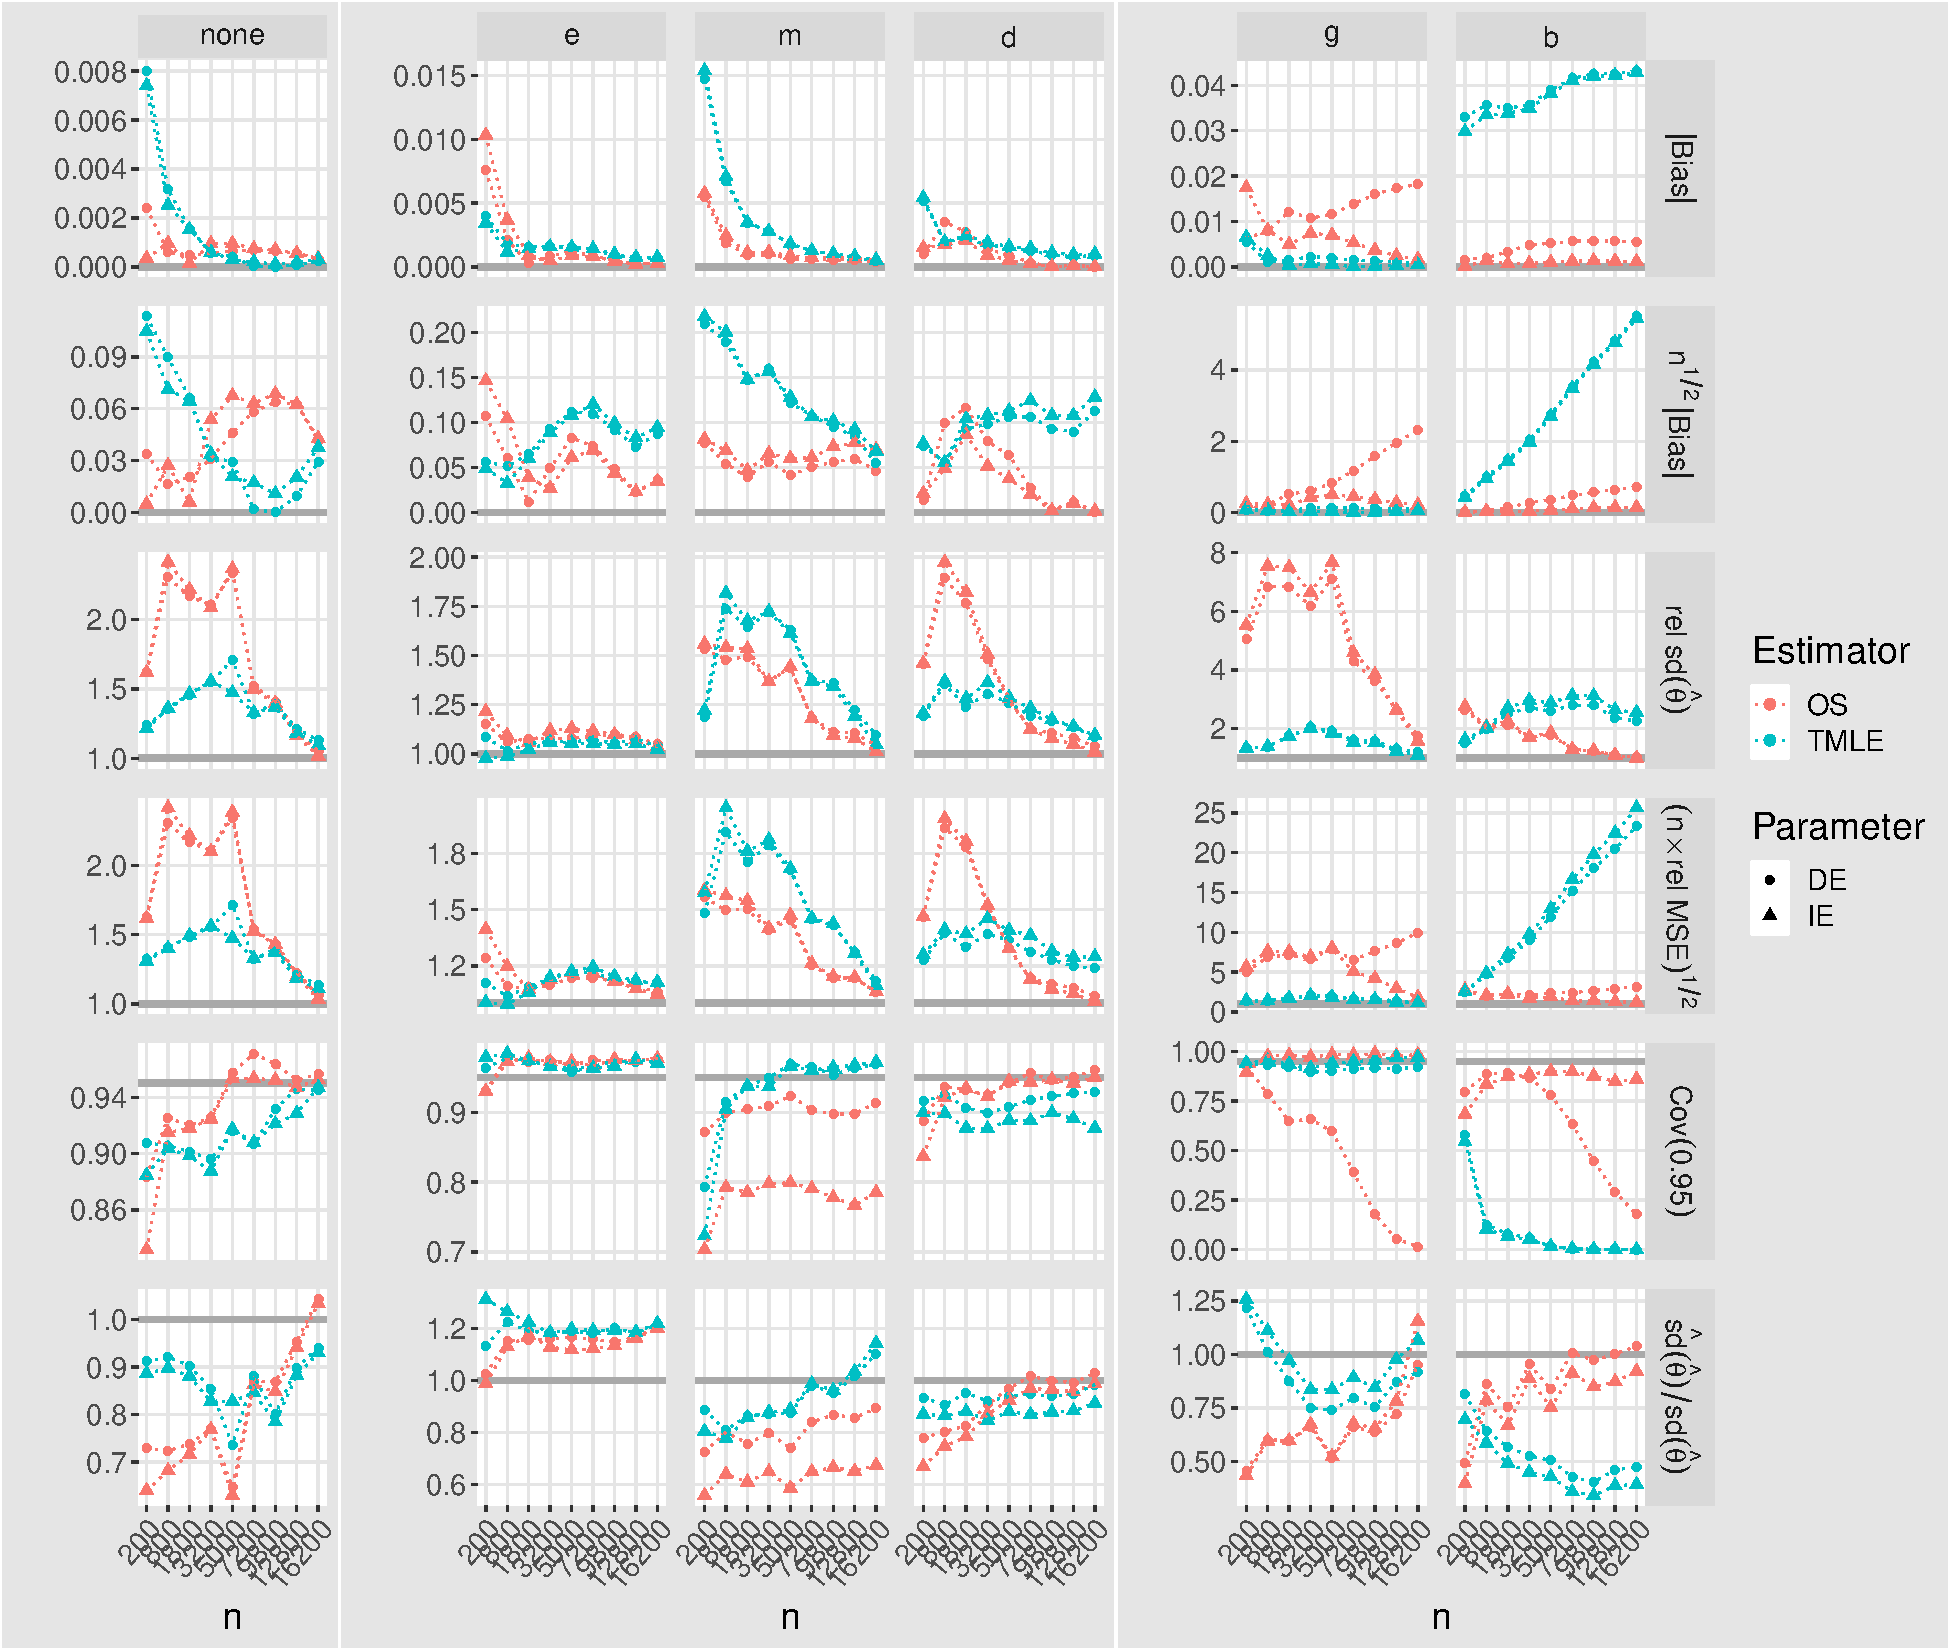
\includegraphics[scale = 0.49]{plot}
  \caption{Comparison of efficient estimators across different nuisance
    parameter configurations.}\label{fig:simula}
\end{figure}
Importantly, the TML estimator appears to generally outperform the one-step
estimator throughout several scenarios. This comes in several forms, including
lower bias, relative standard deviation, or relative mean squared error under
misspecification of $\{\e, \m, \d\}$ or under no misspecification; however,
under inconsistent estimation of $\{\g, \b\}$, the irregularity of the
estimators complicates this comparison. Interestingly, under misspecification of
$\g$, the TML estimators of the direct and indirect effects appear unbiased and
efficient, a result unpredictable from theory given the irregularity of the
estimators under this configuration. Altogether, results of our numerical
experiments indicate that our proposed estimators exhibit properties that align
with the theoretical results of Lemmas~\ref{lemma:dr1} and~\ref{lemma:dr2}.

%%%%%%%%%%%%%%%%%%%%%%%%%%%%%%%%%%%%%%%%%%%%%%%%%%%%%%%%%%%%%%%%%%%%%%%%%%%%%%%
\section{Application to the X:BOT Trial}\label{sec:applic}
%%%%%%%%%%%%%%%%%%%%%%%%%%%%%%%%%%%%%%%%%%%%%%%%%%%%%%%%%%%%%%%%%%%%%%%%%%%%%%%

We now consider the application of our proposed stochastic interventional direct
and indirect effects to decompose the causal effect of a strategy where
buprenorphine dose is successively increased early in treatment (regardless of
opioid use) on relapse among those with opioid use disorder (OUD). Data for our
illustrative analysis come from the X:BOT trial, a 24-week, multi-site
randomized controlled trial designed to examine the comparative effectiveness of
extended-release naltrexone (XR-NTX) and sublingual buprenorphine-naloxone
(BUP-NX) on relapse~\citep{lee2018comparative, lee2016nida, nunes2016ethical}.
The X:BOT trial enrolled 570 participants, all of whom were 18 years or older,
had OUD~\citep[as per the Diagnostic and Statistical Manual of Mental
Disorders-5;][]{apa2013dsm5}, and had used non-prescribed opioids in the 30 days
preceding enrollment. Participants were randomized to receive either XR-NTX or
BUP-NX using a stratified permuted block design; 287 of the 570 were randomized
to receive BUP-NX. Prior analytic efforts have established a protective effect
of BUP-NX administration (versus placebo) on OUD
relapse~\citep{mattick2014buprenorphine}. For each participant assigned to
receive BUP-NX, the prescribed dose was based on both clinical
indication~\citep{lee2018comparative} and clinician judgment. Some clinicians
tended to hold dose constant over time (i.e., a static regimen), while others
increased dose --- either based on clinical assessment or on the hypothesis that
higher doses would result in better outcomes~\citep{nutt2015considerations,
greenwald2003effects, comer2005buprenorphine, heikman2017polydrug}. In this
analysis, we estimated hypothetical stochastic interventional (in)direct effects
to assess the mechanism by which universally ramping up BUP-NX dose early in
treatment (defined as three or more dose increases in the first four weeks of
treatment) could mitigate the risk of OUD relapse.

Baseline covariates ($W$) available in the data included site; gender; age;
race/ethnicity; homeless status; educational attainment; employment status;
marital status; current intravenous drug use; alcohol use disorder; cocaine use
disorder; age at start of heroin use; severity of current opioid use; indicator
of prior OUD treatment; past withdrawal discomfort level; histories of
amphetamine use, sedative use, and cannabis use; weekly cost of primary drug;
whether or not living with an individual currently using drugs or with alcohol
use disorder; histories of psychiatric illnesses; randomization timing; baseline
pain level; baseline depression symptoms. The exposure ($A$) was taken to be
successive increases in dose of BUP-NX versus static dose, measured during the
first four weeks of treatment. Mediating factors ($Z$) included depression and
pain, measured from week 6 until relapse or week 24 (end of follow-up).
Abstinence from illicit opioid use early in the treatment schedule, measured
between weeks 4 and 6, acted as an intermediate confounder affected by exposure
($L$). OUD relapse status at the X:BOT trial's end of follow-up was the outcome
of interest ($Y$). To examine the effect of exposure to successive increases in
BUP-NX dose, we consider an incremental propensity score intervention, which,
for binary $A$, replaces the propensity score $g(1 \mid w)$ with a shifted
variant constructed from multiplying the odds of treatment by a user-specified
parameter $\delta$~\citep{kennedy2019nonparametric}, which we vary along a grid
$\log(\delta) \in \{-10.0, -9.5, \ldots, 9.5, 10.0\}$ of the exposure odds
observed in the X:BOT trial.
%By considering a grid in $\delta$ of plausible incremental propensity score
%interventions, our (in)direct effect estimates are poised to reveal both
%a mechanistic pathway through which adaptive BUP-NX dose can affect OUD
%relapse as well as the interplay of dose strategies (indirectly) with
%pertinent neuropsychiatric sequela.
Across all such estimates in the odds $\delta$ of exposure, the stochastic
interventional (in)direct effects that we estimated may be interpreted
in terms of the overall effect of increasingly encouraging ramping up BUP-NX
dose early in treatment on the counterfactual risk of OUD relapse; thus, the
results of our analysis may be informative of the mechanisms by which increasing
BUP-NX dose can alter the risk of OUD relapse. Figure~\ref{fig:xbot_ipsi}
presents the direct and indirect effect estimates across the grid in $\delta$.
\begin{figure}[H]
  \centering
  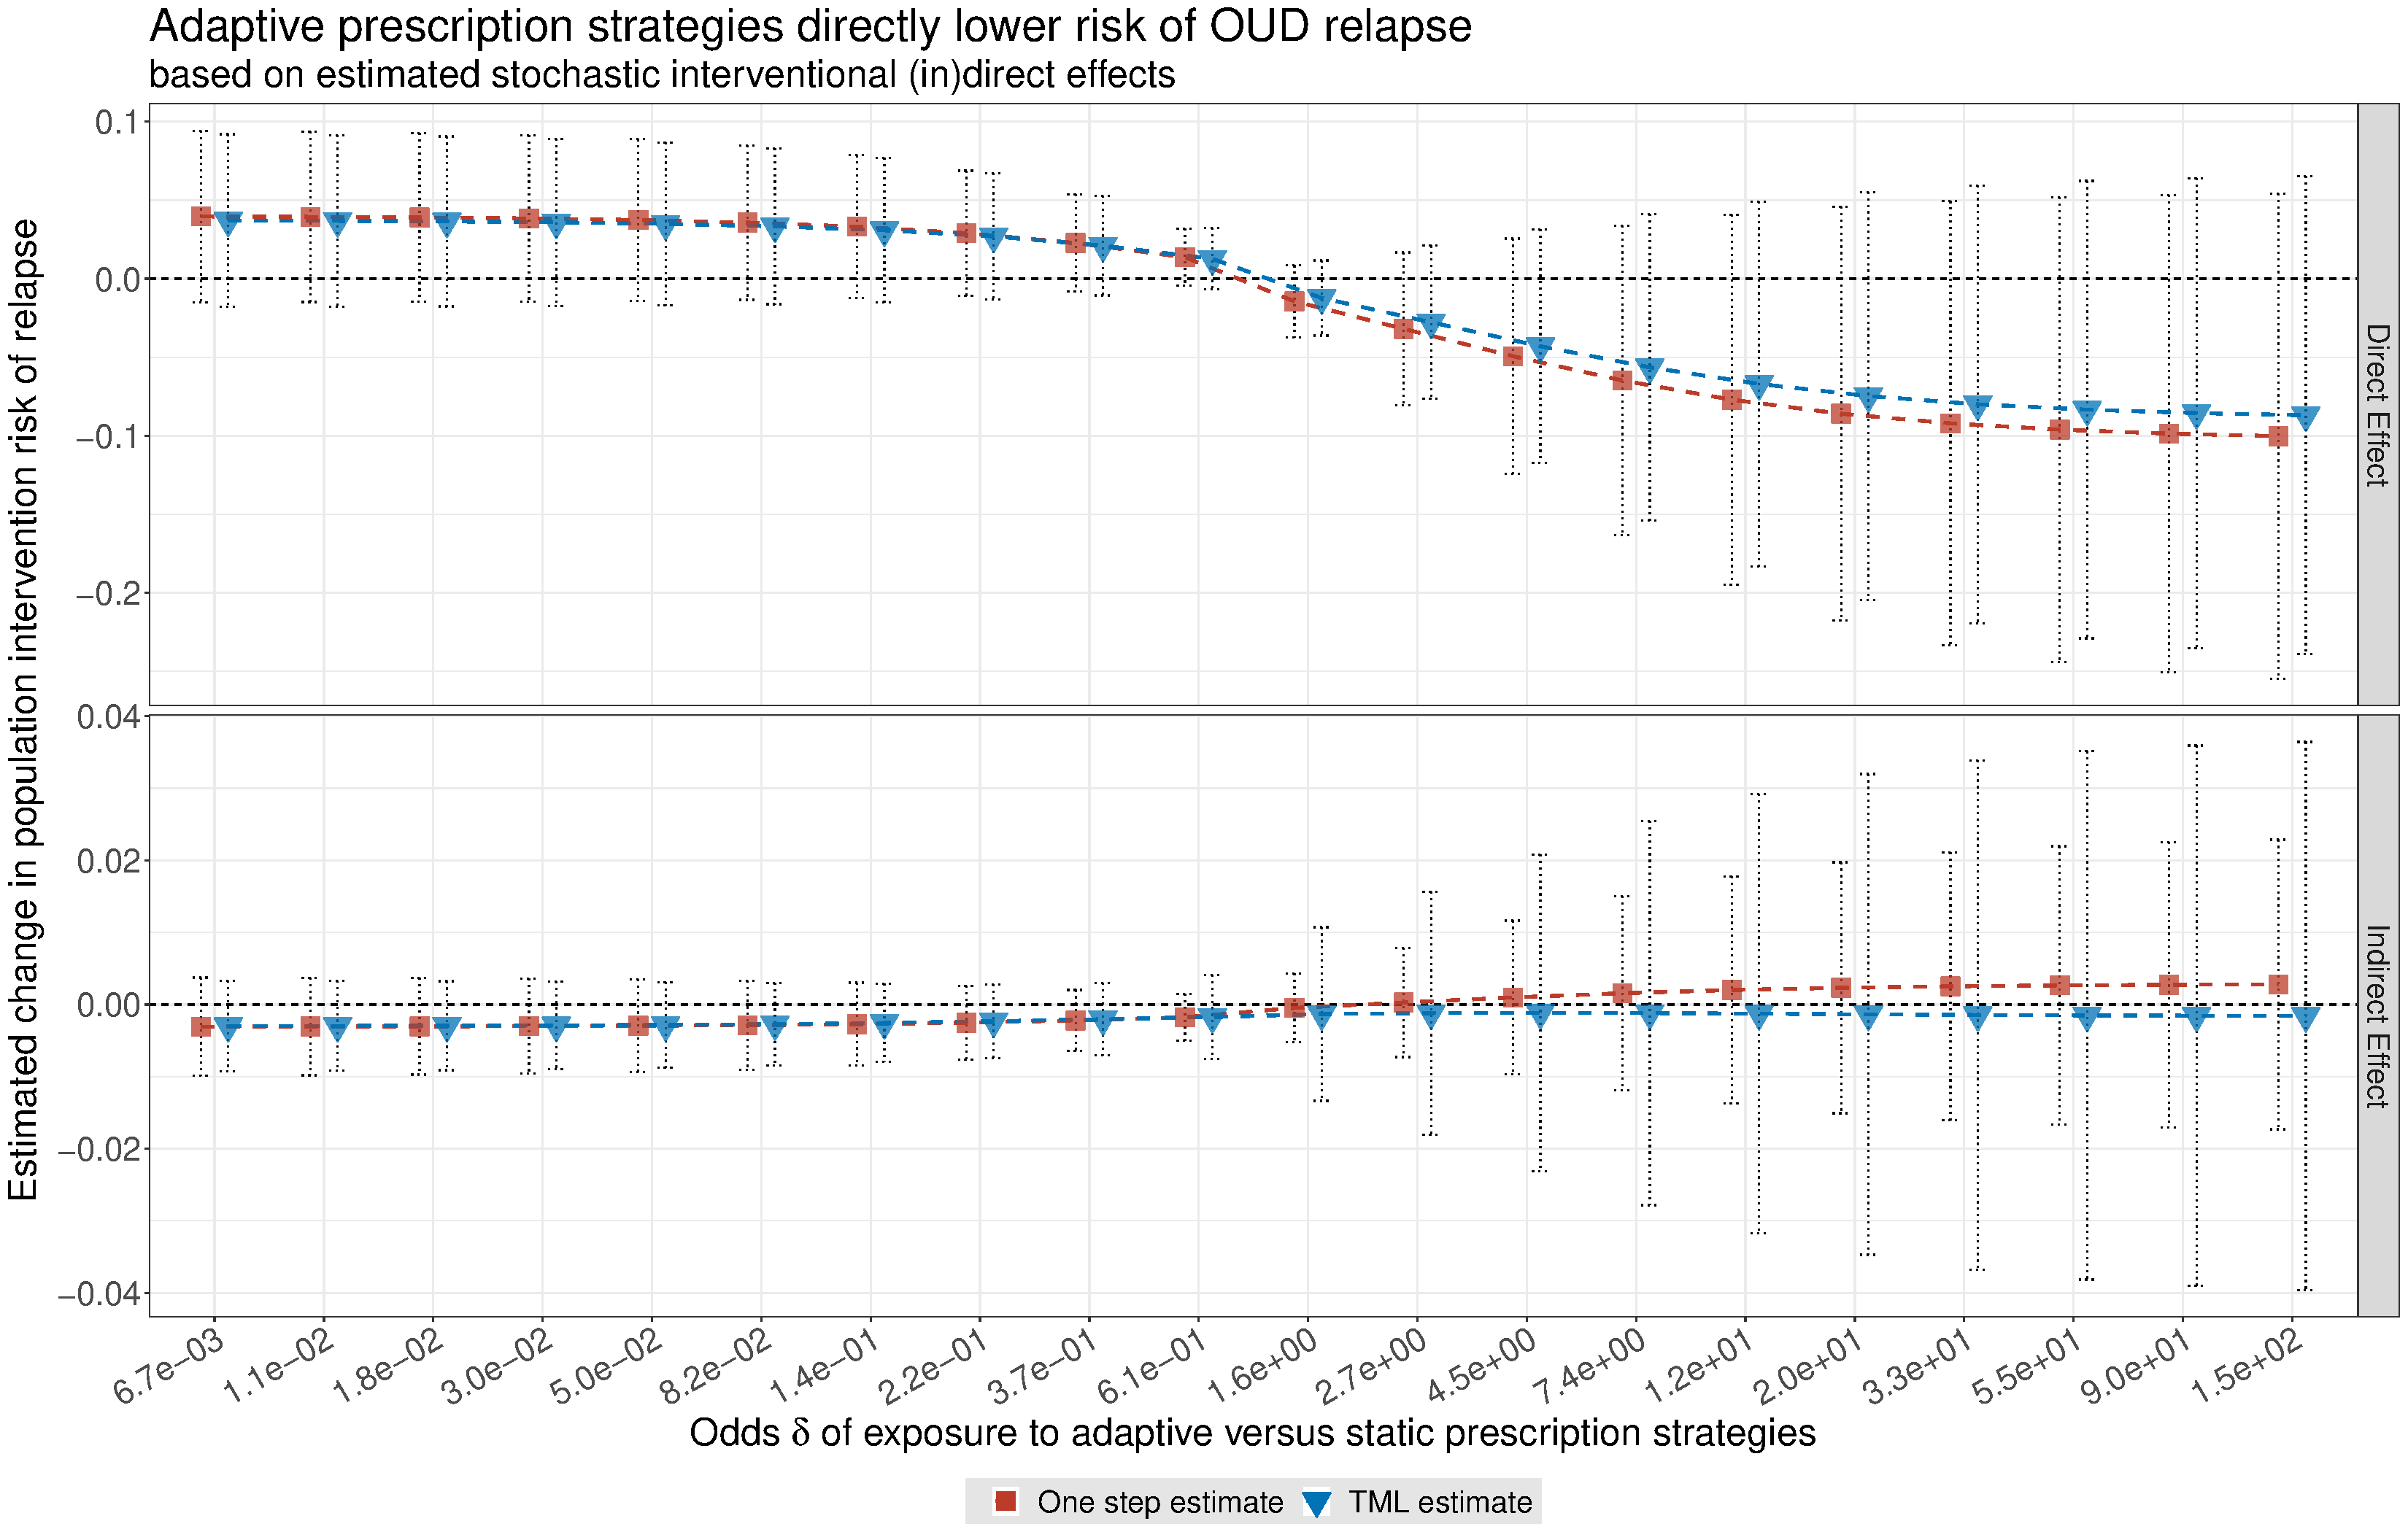
\includegraphics[scale=0.29]{manuscript_xbot}
  \caption{Stochastic interventional direct (upper panel) and indirect (lower
  panel) effect estimates of a hypothetical intervention increasing odds of
  exposure to a BUP-NX dose schedule in which dose is successively increased
  early in OUD relapse treatment across a grid of shifts $\delta$ in the odds.}
  \label{fig:xbot_ipsi}
\end{figure}
We applied both of our cross-fitted, efficient one-step and TML estimators to
examine the stochastic interventional direct and indirect effects of increasing
the odds of ramping up BUP-NX dose. Both estimation strategies produced results
that were generally in very close agreement as to the magnitude of the direct
and indirect effects. For each point estimate, standard error estimates and 95\%
Wald-style confidence intervals were constructed based on the conclusions of
Theorem~\ref{theo:astmle}. In order to ensure the flexibility of our estimators,
each component of the vector of nuisance parameters $\eta = (\e, \m, \d, \g,
\b)$ was estimated via ensemble machine learning, using the Super Learner
algorithm~\citep{vdl2007super, coyle2021sl3}. The library of machine learning
algorithms from which the Super Learner ensemble was constructed included
intercept-only logistic regression, logistic regression with Bayesian priors on
parameters, multivariate adaptive regression
splines~\citep{friedman1991multivariate}, generalized additive
models~\citep{hastie1990generalized}, random forests~\citep{breiman2001random},
gradient boosted machines~\citep{friedman2001greedy}, and the highly adaptive
lasso~\citep{benkeser2016highly, coyle2021hal9001, hejazi2020hal9001}.

From examination of the point estimates and confidence intervals of the direct
and indirect effects in Figure~\ref{fig:xbot_ipsi}, two conclusions may be
drawn. Firstly, there appears to be little to no indirect effect of successively
increasing BUP-NX dose on risk of OUD relapse, revealing that any effect of
BUP-NX dose does not appear to operate through mediating factors such as
depression or pain. Secondly, the direct effect of successively increasing
BUP-NX dose varies considerably across changes in the odds of the introduction
of such a dose schedule. Importantly, it appears that decreasing the odds of
increasing  dose could lead to as much as a 5\% increase in the OUD relapse
risk, with a plateau emerging at odds lower than $\approx$0.1\%, suggesting that
static dose can lead to increased relapse risk relative to successive dose
increases. Continuing this pattern, OUD relapse risk appears to decrease by
$\approx$10\% with increasing odds of successively increasing BUP-NX dose, with
the risk plateauing at odds higher than 33\%. This decrease in the
counterfactual risk of OUD relapse suggests a protective effect of BUP-NX dose
schedules where dose is successively increased early in treatment relative to
static dose.

The conclusions that may be drawn from our re-analysis using the stochastic
interventional direct and indirect effects complement those previously reported
in the investigations of~\citet{lee2018comparative}, who evaluated the total
effect of BUP-NX (versus XR-NTX) treatment on OUD relapse,
and~\citet{rudolph2020explaining}, who used the interventional mediation
analysis approach of~\citet{diaz2020nonparametric} (limited to static
interventions on $A$) to examine differences in relapse risk between homeless
and non-homeless participants. Importantly, our substantive conclusion --- that
dose increases directly lower the risk of relapse --- agree generally with those
of~\citet{rudolph2020association}, who found that dose increases directly
lowered risk of OUD relapse when such dose increases followed opioid use.
Notably, our proposed (in)direct effects and estimation approach differ from
previous efforts in three important ways: (i) our causal effect definitions
remain unaltered in the presence intermediate confounders affected by exposure
and may be re-evaluated in randomized trials, (ii) the flexible estimators we
introduce eschew restrictive modeling assumptions by incorporating
state-of-the-art machine learning in the estimation of nuisance parameters, and
(iii) our strategy provides an analog to a dose-response analysis by allowing
for the risk of OUD relapse to be traced out across changes in the odds of
exposure to a schedule in which BUP-NX dose is increased repeatedly early in
treatment.

%%%%%%%%%%%%%%%%%%%%%%%%%%%%%%%%%%%%%%%%%%%%%%%%%%%%%%%%%%%%%%%%%%%%%%%%%%%%%%%
\section{Discussion}\label{sec:discuss}
%%%%%%%%%%%%%%%%%%%%%%%%%%%%%%%%%%%%%%%%%%%%%%%%%%%%%%%%%%%%%%%%%%%%%%%%%%%%%%%

% Structure adapted from
% https://www.tandfonline.com/doi/pdf/10.1080/01621459.2017.1319839

We have proposed a class of novel direct and indirect effects for causal
mediation analysis, as well as two efficient estimators of these effects in the
nonparametric statistical model. Importantly, our proposed estimation framework
allows for data adaptive estimation of nuisance parameters, while still
preserving the benefits associated with similar classical techniques --- that
is, our estimators are regular and asymptotically linear, provide unbiased point
estimates, are multiply robust, allow the construction of asymptotically valid
confidence intervals, and are capable of attaining the nonparametric efficiency
bound. Our (in)direct effects have interpretations that echo those of the
classical natural (in)direct effects; however, our effects remain well-defined
even in the presence of intermediate confounders affected by exposure. Further,
any scientific conclusions drawn based upon our proposed (in)direct effects may
be readily interrogated in trials that randomize both the exposure and
mediators. Such flexible effect definitions and estimators seem necessary both
to cope with the design complexity exhibited by modern epidemiological and
biomedical studies and to take appropriate advantage of the ever-growing number
of data adaptive regression techniques.

The challenge of leveraging data adaptive regression methodology to construct
robust estimators that accommodate valid statistical inference is not a new one.
It has been considered in great detail as early as the work
of~\citet{pfanzagl1985contributions} as well in numerous recent advances, most
notably by~\citet{vdl2011targeted, vdl2018targeted}
and~\citet{chernozhukov2018double}; related work by these authors presents
a wealth of extensions and applications. In the present work, we derive multiply
robust, efficient estimators based on both the one-step and targeted minimum
loss estimation frameworks. Following~\citet{klaassen1987consistent}
and~\citet{zheng2011cross}, our estimators leverage cross-validation to avoid
imposing possibly restrictive assumptions on nuisance function estimators. We
demonstrated the properties of our estimators in simulation experiments that
illustrated their ability to yield unbiased point estimates, attain the
nonparametric efficiency bound, and build confidence intervals covering at the
nominal rate across several nuisance parameter configurations --- all within a
problem context in which classical mediation effects are ill-defined. We
demonstrated the application of our novel (in)direct effects in dissecting the
mechanism by which increasing odds of adopting a dose schedule of universal
successive increases in buprenorphine dose early in treatment affects OUD
relapse~\citep{lee2018comparative, rudolph2020explaining}.

Several significant extensions and refinements are left for future
consideration. Firstly, our proposed estimation strategy for the direct and
indirect effects leverages re-parameterizations of factors of the likelihood in
order to simplify the estimation of nuisance parameters. This approach works
particularly well when either mediators or intermediate confounders are of low
dimension; however, improving this approach to accommodate moderate
dimensionality of both mediators and intermediate confounders would surely widen
the range of scenarios to which the methodology may be applied. Secondly, when
defining effects based upon stochastic interventions indexed by the
user-specified parameter $\delta$, an important consideration is choosing
\textit{a priori} a particular value of $\delta$. One solution is to evaluate
a set of causal effects indexed by a grid in $\delta$. In such cases, aggregate
effects (across $\delta$) may be summarized via working marginal structural
models~\citep[e.g.,][]{hejazi2020efficient} or the construction of uniform tests
of the null hypothesis of no direct effect~\citep[e.g.,][]{diaz2020causal}.
Developments of these distinct summarization strategies would enrich the range
of scientific problems on which these robust and flexible (in)direct effects may
be brought to bear.

%%%%%%%%%%%%%%%%%%%%%%%%%%%%%%%%%%%%%%%%%%%%%%%%%%%%%%%%%%%%%%%%%%%%%%%%%%%%%%%
\section{Supplementary Material}\label{sm}
%%%%%%%%%%%%%%%%%%%%%%%%%%%%%%%%%%%%%%%%%%%%%%%%%%%%%%%%%%%%%%%%%%%%%%%%%%%%%%%

\subsection{Theorem \ref{theo:iden}}
\begin{proof}
  % The first part of the Theorem is proved in \cite{Diaz12}. The second part
  % is proved as follows.
  First, we have
  \begin{align}
    \E&\{Y_{A_\delta, G_\delta}\} \notag\\&= \int \E\left\{Y_{a,z}\mid
                                            A_\delta=a,G_\delta = z,
                                            W=w\right\}\g_\delta(a\mid
                                            w)\P(G_\delta=z\mid
                                            A_\delta=a,W=w)\p(w)\dd\nu(a,z,w)\notag\\
      &= \int \E\left\{Y_{a,z}\mid W=w\right\}\g_\delta(a\mid
        w)\P(Z(a)=z\mid
        A_\delta=a,W=w)\p(w)\dd\nu(a,z,w)\label{eq:t1e1}\\
      &= \int \E\left\{Y_{a,z}\mid A=a,W=w\right\}\g_\delta(a\mid
        w)\P(Z(a)=z\mid W=w)\p(w)\dd\nu(a,z,w)\label{eq:t1e2}\\
      &= \int \E\left\{Y_{a,z}\mid A=a,W=w\right\}\g_\delta(a\mid
        w)\P(Z(a)=z\mid A=a,W=w)\p(w)\dd\nu(a,z,w)\label{eq:t1e3}\\
      &= \int \E\left\{Y_{a,z}\mid A=a,W=w,L=l\right\}\b(l\mid a,w)\g_\delta(a\mid
        w)\p(z\mid a,w)\p(w)\dd\nu(a,z,l,w)\notag\\
      &= \int \m(a,z,l,w)\b(l\mid a,w)\g_\delta(a\mid
        w)\p(z\mid a,w)\p(w)\dd\nu(a,z,l,w)\label{eq:t1e4},
  \end{align}
  where (\ref{eq:t1e1}) follows by definition of $(A_\delta,G_\delta)$,
  (\ref{eq:t1e2}) follows by~\ref{ass:ncay} and definition of
  $A_\delta$, (\ref{eq:t1e3}) follows by~\ref{ass:ncaz}, and
  (\ref{eq:t1e4}) follows by~\ref{ass:nczy}. Similar arguments yield
  \[\E\{Y_{A, G}\}=\int \m(a,z,l,w)\b(l\mid a,w)\g(z\mid
    w)\p(z\mid a,w)\p(w)\dd\nu(a,z,l,w).\]
  We also have
  \begin{align*}
    \E&\{Y_{A_\delta, G}\} \notag\\&= \int \E\left\{Y_{a,z}\mid
                                     A_\delta=a,G = z,
                                     W=w\right\}\g_\delta(a\mid
                                     w)\P(G=z\mid
                                     A_\delta=a,W=w)\p(w)\dd\nu(a,z,w)\notag\\
      &= \int \E\left\{Y_{a,z}\mid W=w\right\}\g_\delta(a\mid
        w)\P(G=z\mid W=w)\p(w)\dd\nu(a,z,w)\\
      &= \int \E\left\{Y_{a,z}\mid A=a,W=w\right\}\g_\delta(a\mid
        w)\p(z\mid w)\p(w)\dd\nu(a,z,w)\\
      &= \int \E\left\{Y_{a,z}\mid A=a,W=w\right\}\g_\delta(a\mid
        w)\p(z\mid w)\p(w)\dd\nu(a,z,w)\\
      &= \int \E\left\{Y_{a,z}\mid A=a,W=w,L=l\right\}\b(l\mid a,w)\g_\delta(a\mid
        w)\p(z\mid w)\p(w)\dd\nu(a,z,l,w)\notag\\
      &= \int \m(a,z,l,w)\b(l\mid a,w)\g_\delta(a\mid
        w)\p(z\mid w)\p(w)\dd\nu(a,z,l,w).
  \end{align*}
  Subtracting gives the expressions for the PIIE and PIDE in the
  theorem.
\end{proof}

\subsection{Efficient Influence Functions (Theorem~\ref{theo:eif})}
\begin{proof}
  In this proof we will use $\Theta_j(\P):j=1,2$ to denote a parameter
  as a functional that maps the distribution $\P$ in the model to a
  real number. We will assume that the measure $\nu$ is discrete so
  that integrals can be written as sums, and will omit the dependence
  on $\delta$. It can be checked algebraically that the resulting
  influence function will also correspond to the influence function of
  a general measure $\nu$. The true parameter value for $\theta_1$ is
  thus given by
  \[\theta_1=\Theta_1(\P) = \sum_{y,a,z,m,w} y\,\p(y\mid a, z, l,
    w)\p(l\mid a,w)\p(z\mid a,w)\g_\delta(a\mid w)\p(w).\] The
  non-parametric MLE of $\theta_1$ in the model of $\g_\delta$ known
  is given by
  \begin{equation}
    \Theta(\Pn)=\sum_{y,a,z,m,w}y\frac{\Pn f_{y,a,z,l,w}}{\Pn
      f_{a,z,l,w}}\frac{\Pn f_{l,a,w}}{\Pn f_{a,w}}\frac{\Pn
      f_{z,a,w}}{\Pn f_{a,w}}\g_{\delta}(a\mid w)\Pn f_w\label{nonpest},
  \end{equation}
  where we remind the reader of the notation $\P f =\int f \dd\P$. Here
  $f_{y,a,z,l,w}=\one(Y=y,A=a,Z=z,M=m,W=w)$, and $\one(\cdot)$ denotes
  the indicator function. The other functions $f$ are defined
  analogously.

  We will use the fact that the efficient influence function in a
  non-parametric model corresponds with the influence curve of the
  NPMLE. This is true because the influence curve of any regular
  estimator is also a gradient, and a non-parametric model has only
  one gradient. The Delta method \cite[see, e.g., Appendix 18
  of][]{vdl2011targeted} shows that if $\hat \Theta_1(\Pn)$ is a
  substitution estimator such that $\theta_1=\hat \Theta_1(\P)$, and
  $\hat \Theta_1(\Pn)$ can be written as
  $\hat \Theta^*_1(\Pn f:f\in\mathcal{F})$ for some class of functions
  $\mathcal{F}$ and some mapping $\Theta^*_1$, the influence function of
  $\hat \Theta_1(\Pn)$ is equal to
  \[\dr_\P(O)=\sum_{f\in\mathcal{F}}\frac{\dd\hat \Theta^*_1(\P)}
  {\dd\P f}\{f(O)-\P f\}.\]

  Applying this result to (\ref{nonpest}) with
  $\mathcal{F}=\{f_{y,a,z,l,w},f_{a,z,l,w},f_{z,a,w},f_{a',w},
  f_{l,a,w},f_{a,w},f_w:y,a,z,l,w\}$ and rearranging terms gives the result of
  the theorem. The algebraic derivations involved here are lengthy and not
  particularly illuminating, and are therefore omitted from the proof. Similar
  analyses may be performed for the model where only $\g_\delta$ is unknown, as
  well as $\theta_2$.
\end{proof}

\subsection{Targeted Minimum Loss Estimation Algorithm}

To simplify notation, in the remaining of this section we will denote
$\tilde \eta_{j(i)}(O_i)$ with $\tilde \eta(O_i)$. If $L$ is binary,
the efficient influence functions in Theorem~\ref{theo:eif} may be
simplified using the following identity:
\[ \vv(l,a,w) - \bar\vv(a,w) = \{\vv(1,a,w) -\vv(0,a,w)\}
\{l-\b(1\mid a, w)\},\] which also holds for $\vv$ replaced by $\s$ and
$\bar\vv$ by $\bar\s$.

\begin{enumerate}[label=Step \arabic*., align=left, leftmargin=*]
\item Initialize $\tilde\eta =\hat\eta$. Compute $\tilde\vv$,
  $\tilde\s$, and $\tilde\q^j$ by plugging in $\tilde \m$,
  $\tilde \g$, $\tilde \e$, $\tilde \d$ into equations~\eqref{eq:nuis},
  \eqref{eq:altnuis} and~\eqref{eq:defqs} if
  $Z$ is multivariate, and fitting data-adaptive regression algorithms as
  appropriate.

\item \label{step:computeH} For each subject, compute the auxiliary covariates
  \begin{align*}
    H_{\mbox{\scriptsize D}, i} &= \frac{{\tilde\b}(L_i\mid A_i,
                                  W_i)}{{\tilde\d}(L_i \mid Z_i, A_i,
                                  W_i)}\left\{1-\frac{{\tilde\g}_\delta(A_i\mid
                                  W_i)}{{\tilde\e}(A_i\mid Z_i,W_i)}\right\}\\
    H_{\mbox{\scriptsize I}, i} &= \frac{{\tilde\b}(L_i\mid A_i,
                                  W_i)}{{\tilde\d}(L_i \mid Z_i, A_i,
                                  W_i)}\left\{\frac{{\tilde\g}_\delta(A_i\mid
                                  W_i)}{{\tilde\e}(A_i\mid
                                  Z_i,W_i)}-\frac{\tilde{\g}_\delta(A_i
                                  \mid W_i)}{{\tilde\g}(A_i\mid
                                  W_i)}\right\}\\
    K_{\mbox{\scriptsize D}, i} & = {\tilde\vv}(1,A_i,W_i)
                                  - {\tilde\vv}(0,A_i,W_i) - \frac{{\tilde\g}_\delta(A_i
                                  \mid W_i)}{{\tilde\g}(A_i\mid W_i)} \{{\tilde\s}(1,A_i,W_i) -
                                  {\tilde\s}(0,A_i,W_i)\}\\
    K_{\mbox{\scriptsize I}, i} & = \frac{{\tilde\g}_\delta(A_i
                                  \mid W_i)}{{\tilde\g}(A_i\mid W_i)}
                                  \{{\tilde\s}(1,A_i,W_i) -
                                  {\tilde\s}(0,A_i,W_i) - {\tilde\vv}(1,A_i,W_i)
                                  + {\tilde\vv}(0,A_i,W_i)\}\\
    M_{\mbox{\scriptsize D}, i} & = -\frac{\tilde\g_\delta(1\mid w)(1 -
                                  \tilde\g_\delta(1\mid w))}{\tilde\g(1\mid w)(1 -
                                  \tilde\g(1\mid w))}{\tilde\q}^2(w)\\
    M_{\mbox{\scriptsize I}, i} & = \frac{\tilde\g_\delta(1\mid w)(1 -
                                  \tilde\g_\delta(1\mid w))}{\tilde\g(1\mid w)(1 -
                                  \tilde\g(1\mid w))}\{{\tilde\q}^2(w)-{\tilde\q}^1(w)\}
  \end{align*}
\item \label{step:fit} Fit the logistic tilting models
  \begin{align*}
    \logit \m_\beta(A_i,Z_i,L_i,W_i) &= \logit \tilde
                                       \m(A_i,Z_i,L_i,W_i) + \beta_I H_{\mbox{\scriptsize I}, i} +
                                       \beta_D H_{\mbox{\scriptsize D}, i}\\
    \logit \b_\alpha(1\mid A_i,W_i) &= \logit \tilde
                                      \b(1\mid A_i,W_i) + \alpha_I K_{\mbox{\scriptsize I}, i} +
                                      \alpha_D K_{\mbox{\scriptsize
                                      D}, i}\\
    \logit \g_\gamma(1\mid W_i) &= \logit \tilde
                                  \g(1\mid W_i) + \gamma_I M_{\mbox{\scriptsize I}, i} +
                                  \gamma_D M_{\mbox{\scriptsize D}, i}
  \end{align*}
  where
  $\logit(p) = \log\{p(1-p)^{-1}\}$. Here, $\logit \tilde\m(a,z,l,w)$
  is an offset variable (i.e., a variable with known parameter value
  equal to one). The parameter $\beta=(\beta_I, \beta_D)$ may be
  estimated by running standard logistic regression of $Y_i$ on
  $(H_{\mbox{\scriptsize D}, i}, H_{\mbox{\scriptsize I}, i})$ with no
  intercept and an offset term equal to
  $\logit \tilde\m(A_i,Z_i,L_i,W_i)$. Let $\hat\beta$ denote the
  estimate, and let $\tilde \m=\m_{\hat\beta}$ denote the updated
  estimates. Perform analogous computations for $\b$ and $\g$.
\item \label{step:computeu} Compute $\tilde\uu$ according to
   equation~\eqref{eq:nuis} by plugging in $\tilde\m$ and $\tilde\b$. Compute
  the covariate
  \[J_i = \frac{{\tilde\g}_\delta(A_i
      \mid W_i)}{{\tilde\g}(A_i\mid W_i)},\]
  and fit the model
  \[\logit \bar\uu_\kappa(A_i,W_i) = \logit \tilde{\bar\uu}(A_i,W_i) +
    \kappa_D + \kappa_I J_{ i}\] by running a logistic regression of
  $\tilde\uu(Z_i,A_i,W_i)$ on $J_i$ with an intercept and offset
  $\logit \tilde{\bar\uu}(A_i,W_i)$. Let $\hat\kappa$ denote the MLE,
  and update $\tilde{\bar\uu} = \bar\uu_{\hat \kappa}$.
\item The TMLE of the direct and indirect effects are defined as:
  \begin{equation*}
    \begin{split}
      \psidtmle &= \frac{1}{n} \int\sum_{i = 1}^n
      \left\{\tilde{\bar\uu}(a,W_i)\tilde\g(a\mid W_i) -
        \tilde\uu(Z_i,a,W_i)\tilde\g_\delta(a\mid W_i)\right\}\dd\kappa(a)\\
      \psiitmle &= \frac{1}{n} \int\sum_{i = 1}^n
      \left\{\tilde\uu(Z_i,a,W_i) -
        \tilde{\bar\uu}(a,W_i)\right\}\tilde\g_\delta(a\mid
      W_i)\dd\kappa(a)
    \end{split}
  \end{equation*}
\end{enumerate}

\subsection{Proof of Theorem \ref{theo:asos}}
\begin{proof}
  Let $\Pnj$ denote
  the empirical distribution of the prediction set ${\cal V}_j$, and let
  $\Gnj$ denote the associated empirical process
  $\sqrt{n/J}(\Pnj-\P)$. For simplicity we denote a general parameter
  $\psi$ with influence function $D_\eta$, the proof applies equally
  to the direct and indirect effect parameters. Note that
  \[\psios = \frac{1}{J}\sum_{j=1}^J\Pnj D_{\hat
      \eta_j,\delta},\,\,\,\psi_\delta=\P D_{\eta}.\]Thus,
  \[  \sqrt{n}\{\psios - \psi_\delta\}=\Gn \{D_{\eta,\delta}
    - \psi_\delta\} + R_{n,1}(\delta) + R_{n,2}(\delta),\]
  where
  \[  R_{n,1}(\delta)  =\frac{1}{\sqrt{J}}\sum_{j=1}^J\Gnj(D_{\hat
      \eta_j,\delta} - D_{\eta,\delta}),\,\,\,
    R_{n,2}(\delta)  = \frac{\sqrt{n}}{J}\sum_{j=1}^J\P\{D_{\hat
      \eta_j,\delta}-\psi_\delta\}.
  \]
  It remains to show that $R_{n,1}(\delta)$ and $R_{n,2}(\delta)$ are
  $o_P(1)$. Lemmas~\ref{lemma:dr1} and~\ref{lemma:dr2} together
  with the Cauchy-Schwartz inequality and assumption \ref{ass:sec1}
  of the theorem shows that $||R_{n,2}||_{\Delta}=o_P(1)$. For
  $||R_{n,1}||_{\Delta}$ we use empirical process theory to argue conditional
  on the training sample ${\cal T}_j$. In particular, Lemma 19.33
  of~\cite{vdvaart2000asymptotic} applied to the class of functions
  ${\cal F} = \{D_{\hat \eta_j,\delta} - D_{\eta,\delta}\}$ (which
  consists of one element) yields
  \[E\left\{\big|\Gnj (D_{\hat \eta_j,\delta} - D_{\eta,\delta})\big|
      \,\bigg|\, {\cal T}_j\right\}\lesssim \frac{2C\log 2}{n^{1/2}} +
    ||D_{\hat \eta_j,\delta} - D_{\eta,\delta}||(\log 2)^{1/2}\] By
  assumption \ref{ass:sec1}, the left hand side is $o_P(1)$. Lemma 6.1
  of~\cite{chernozhukov2018double} may now be used to argue that
  conditional convergence implies unconditional convergence, concluding
  the proof.
\end{proof}

\subsection{Theorem~\ref{theo:astmle}}
\begin{proof}
  Let $\Pnj$ denote the empirical distribution of the prediction set
  ${\cal V}_j$, and let $\Gnj$ denote the associated empirical process
  $\sqrt{n/J}(\Pnj-\P)$. For simplicity we denote a general parameter
  $\psi$ with influence function $D_\eta$, the proof applies equally
  to the direct and indirect effect parameters. By definition, the sum
  of the scores of the submodels
  $\{\m_\beta,\b_\alpha,\g_\gamma,\bar\uu_\kappa:(\beta,\alpha,
  \gamma, \kappa)\}$ at the last iteration of the TMLE procedure is
  equal to
  $n^{-1}\sum_{i=1}^n D_{\tilde \eta}(O_i) = o_P(n^{-1/2})$. Thus, we have
  \[\psitmle = \frac{1}{J}\sum_{j=1}^J\Pnj D_{\tilde \eta_j}+o_P(n^{-1/2}).\]
  Thus,
  \[  \sqrt{n}(\psitmle - \theta)=\Gn (D_{\eta}
    - \theta) + R_{n,1} + R_{n,2} + o_P(n^{-1/2}),\]
  where
  \[  R_{n,1}  =\frac{1}{\sqrt{J}}\sum_{j=1}^J\Gnj(D_{\tilde
      \eta_j} - D_{\eta}),\,\,\,
    R_{n,2}  = \frac{\sqrt{n}}{J}\sum_{j=1}^J\P(D_{\tilde
      \eta_j}-\theta).
  \]
  As in the proof of Theorem~\ref{theo:asos}, Lemmas~\ref{lemma:dr1}
  and~\ref{lemma:dr2} together with the Cauchy-Schwartz inequality and
  the assumptions of the theorem shows that $R_{n,2}=o_P(1)$.

  Since $D_{\tilde \eta_j}$ depends on the full sample through the
  estimates of the parameters $\beta$ of the logistic tilting models,
  the empirical process treatment of $R_{n,1}$ needs to be slightly
  from that in the proof of Theorem~\ref{theo:asos}. To make this
  dependence explicit, we introduce the notation
  $D_{\hat \eta_j,\beta}=D_{\tilde \eta_j}$ and $R_{n,1}(\beta)$. Let
  ${\cal F}_n^j=\{D_{\hat \eta_j,\beta} -
  D_\eta:\beta\in B\}$. Because the function
  $\hat\eta_j$ is fixed given the training data, we can apply Theorem
  2.14.2 of~\cite{vdvaart1996weak} to obtain
  \[E\left\{\sup_{f\in {\cal F}_n^j}|\Gnj f| \,\,\bigg|\,\, {\cal
        T}_j\right\}\lesssim ||F^j_n||\int_0^1\sqrt{1+N_{[\,]}(\epsilon
      ||F_n^j||, {\cal F}_n^j, L_2(\P))}\dd\epsilon, \] where
  $N_{[\,]}(\epsilon ||F_n^j||, {\cal F}_n^j, L_2(\P))$ is the
  bracketing number and we take
  $F_n^j=\sup_{\beta\in B}|D_{\hat \eta_j,\beta} -
  D_\eta|$ as an envelope for the class ${\cal
    F}_n^j$. Theorem 2.7.2 of~\cite{vdvaart1996weak} shows
  \[\log N_{[\,]}(\epsilon ||F_n^j||, {\cal F}_n^j, L_2(\P))\lesssim
    \frac{1}{\epsilon ||F_n^j||}.\]
  This shows
  \begin{align*}||F^j_n||\int_0^1\sqrt{1+N_{[\,]}(\epsilon
    ||F_n^j||, {\cal F}_n^j, L_2(\P))}\dd\epsilon &\lesssim
        \int_0^1\sqrt{||F^j_n||^2+\frac{||F^j_n||}{\epsilon}}\dd\epsilon\\
        &\leq
    ||F^j_n||+||F^j_n||^{1/2}\int_0^1\frac{1}{\epsilon^{1/2}}\dd\epsilon\\
        &\leq ||F^j_n|| + 2 ||F^j_n||^{1/2}.
  \end{align*}
  Since $||F^j_n||=o_P(1)$, this shows
  $\sup_{f\in {\cal F}_n^j}\Gnj f=o_P(1)$ for each $j$, conditional on
  ${\cal T}_j$. Thus $\sup_{\beta\in B} R_{n,1}(\beta)=o_P(1)$.
  Lemmas~\ref{lemma:dr1} and~\ref{lemma:dr2} together with the
  Cauchy-Schwartz inequality and the assumptions of the theorem show
  that $R_{n,2}=o_P(1)$, concluding the proof of the theorem.
\end{proof}

\subsection{Additional Results}

\begin{lemma}[Second order terms for modified treatment
  policies]\label{lemma:so1}
  Let $\dd\xi(o)$ denote $\dd\nu(a,l,z)\dd\P(w)$, and let $\r(z\mid,
  a, w)$ denote $\p(z\mid a, w)$, and let $\h(z\mid,
  w)$ denote $\p(z\mid w)$. Let $d(a,w)$ denote a modified treatment
  policy satisfying~\ref{ass:inv}. We have
  \begin{align}
    \P D_{\eta_1,\delta}^1 -\psi_1(\delta) & =
         \int\left(\frac{\g}{\g_1}\frac{\d}{\d_1} -
        1\right)(\m-\m_1)\b_1\r\g_{\delta,1}\dd\xi\label{eq:so1}\\
        &-\int\left(\frac{\g}{\g_1}-1\right)(\bar\uu_1-\bar\uu)
        \g_{\delta,1}\dd\xi\label{eq:so3}\\
         &+\int\left(\frac{\g}{\g_1}-1\right)(\m_1-\m)\b_1\r
         \g_{\delta,1}\dd\xi\label{eq:so4}\\
         &-\int\frac{\g}{\g_1}(\b_1-\b)(\vv_1-\vv)\g_{\delta,1}
         \dd\xi\label{eq:so5}\\
        &-\int(\bar\uu_1-\bar\uu)(\g_{\delta,1}-\g_\delta)
        \dd\xi\label{eq:so2}
  \end{align}
  and
  \begin{align*}
    \P D_{\eta_1,\delta}^2 - \psi_2(\delta)
    & = \int\left(\frac{\e}{\e_1}\frac{\d}{\d_1} -
      1\right)(\m-\m_1)\b_1\h\g_{\delta,1} \dd\xi\\
    &+\int\frac{\g}{\g_1}(\b_1-\b)(\s_1-\s)\g_{\delta,1}\dd\xi\\
    &-\int(\q_1-\q)(\g_{\delta,1}-\g_\delta)\dd\xi.
  \end{align*}
\end{lemma}
\begin{proof} Note that
\begin{equation}
  \begin{split}
    \P S_{\eta_1,\delta}^1 -
    \psi_1(\delta)
    & =
      \int\left(\frac{\g}{\g_1}\frac{\d}{\d_1}
      - 1\right)(\m-\m_1)\b_1\r\g_{\delta,1}\dd\xi
      + \int(\m-\m_1)\b_1\r\g_{\delta,1}\dd\xi                                  \\
    & - \int\bar\uu
      (\g_\delta - \g_{\delta,1})\dd\xi - \int \bar\uu
      \g_{\delta,1}\dd\xi                                                       \\
    & +\int
      \frac{\g}{\g_1}(\b-\b_1)\vv_1\g_{\delta,1}\dd\xi
      + \int
      \frac{\g}{\g_1}(\uu_1\r-\bar\uu_1)\g_{\delta,1}\dd\xi
      +\int\bar\uu_1\g_{\delta,1}\dd\xi                                         \\
    & =(\ref{eq:so1})
      +\int (\bar\uu_1-\bar\uu)\g_{\delta,1}\dd\xi                              \\
    & +\int(\m-\m_1)\b_1\r\g_{\delta,1}\dd\xi +
      \int\frac{\g}{\g_1}(\b-\b_1)\vv_1\g_{\delta,1}\dd\xi                      \\
    & + \int
      \frac{\g}{\g_1}\uu_1\r\g_{\delta,1}\dd\xi
      -\int
      \frac{\g}{\g_1}\bar\uu_1\g_{\delta,1}\dd\xi                               \\
    & - \int\bar\uu
      (\g_\delta - \g_{\delta,1})\dd\xi           \\
    & =(\ref{eq:so1})
      -\int\left(\frac{\g}{\g_1}-1\right)(\bar\uu_1-\bar\uu)\g_{\delta,1}\dd\xi \\
    & +\int \frac{\g}{\g_1}\m_1\b_1\r\g_{\delta,1}\dd\xi - \int
      \frac{\g}{\g_1}\m\b\r\g_{\delta,1}\dd\xi                                  \\
    & +\int(\m-\m_1)\b_1\r\g_{\delta,1}\dd\xi +
      \int\frac{\g}{\g_1}(\b-\b_1)\vv_1\g_{\delta,1}\dd\xi                      \\
    & - \int\bar\uu
      (\g_\delta - \g_{\delta,1})\dd\xi           \\
    & =(\ref{eq:so1})-
      (\ref{eq:so3}) \\
    & +\int(\m-\m_1)\b_1\r\g_{\delta,1}\dd\xi +
      \int\frac{\g}{\g_1}(\b-\b_1)\vv_1\g_{\delta,1}\dd\xi            \\
    & +\int
      \frac{\g}{\g_1}(\m_1\b_1
      +\m\b_1-\m\b_1-
      \m\b)\r\g_{\delta,1}\dd\xi                                      \\
    & - \int\bar\uu
      (\g_\delta - \g_{\delta,1})\dd\xi \\
    & =(\ref{eq:so1}) - (\ref{eq:so3})                                                  \\
    & +
      \int(\m-\m_1)\b_1\r\g_{\delta,1}\dd\xi +
      \int\frac{\g}{\g_1}(\b-\b_1)\vv_1\g_{\delta,1}\dd\xi            \\
    & +\int
      \frac{\g}{\g_1}(\m_1
      -\m)\b_1\r\g_{\delta,1}\dd\xi
      +\int
      \frac{\g}{\g_1}(\b_1-\b)\m\r\g_{\delta,1}\dd\xi                 \\
    & - \int\bar\uu
      (\g_\delta - \g_{\delta,1})\dd\xi \\
    & =(\ref{eq:so1})-(\ref{eq:so3}) +(\ref{eq:so4})-(\ref{eq:so5}) \\
    & - \int\bar\uu(\g_\delta - \g_{\delta,1})\dd\xi.
  \end{split}\label{eq:proof1}
\end{equation}
Using~\ref{ass:inv} we can change variables to obtain
\[\P S_{\eta_1,\delta}^{A,1} =
  \int\bar\uu_1(\g_\delta-\g_{\delta,1})\dd\xi.\] The proof for
$\psi_2$ is analogous. This completes the
proof of the theorem.
\end{proof}

\begin{lemma}[Second order terms for
  exponential tilting.]\label{lemma:so2}
  Define $c(w) = \{\int_a \exp(\delta a)\g(a\mid w)\}^{-1}$, and let
  $c_1(w)$ be defined analogously. Let $b(a) = \exp(\delta a)$. Using
  the same notation as in Lemma~\ref{lemma:dr1}, we have
  \begin{align*}
    \P D_{\eta_1,\delta}^1  -\psi_1(\delta)
    & =
      \int\left(\frac{\g}{\g_1}\frac{\d}{\d_1} -
      1\right)(\m-\m_1)\b_1\r\g_{\delta,1}\dd\xi\\
    &-\int\left(\frac{\g}{\g_1}-1\right)(\bar\uu_1-\bar\uu)\g_{\delta,1}\dd\xi\\
    &+\int\left(\frac{\g}{\g_1}-1\right)(\m_1-\m)\b_1\r\g_{\delta,1}\dd\xi\\
    &-\int\frac{\g}{\g_1}(\b_1-\b)(\vv_1-\vv)\g_{\delta,1}\dd\xi\\
    &+ \int(\bar\uu_1-\bar\uu)(\g_{\delta,1}-\g_\delta)\dd\xi\\
    & -\int\left\{(c_1-c)^2\int b
      \g_1\bar\uu_1\dd\kappa\int b
      \g\dd\kappa\right\}\dd\xi\\
    &+\int \left\{(c_1-c)\int b\bar\uu_1(\g-\g_1)\dd\kappa\right\}\dd\xi,
  \end{align*}
  and
  \begin{align*}
    \P D_{\eta_1,\delta}^2  -\psi_2(\delta)
    & = \int\left(\frac{\e}{\e_1}\frac{\d}{\d_1}  -
      1\right)(\m-\m_1)\b_1\h\g_{\delta,1} \dd\xi\\
    &+\int\frac{\g}{\g_1}(\b_1-\b)(\s_1-\s)\g_{\delta,1}\dd\xi\\
    &-\int(\q_1-\q)(\g_{\delta,1}-\g_\delta)\dd\xi\\
    & -\int\left\{(c_1-c)^2\int b
      \g_1\bar\q_1\dd\kappa\int b
      \g\dd\kappa\right\}\dd\xi\\
    &+\int \left\{(c_1-c)\int b\bar\q_1(\g-\g_1)\dd\kappa\right\}\dd\xi.
  \end{align*}

\end{lemma}

\begin{proof}
  In this proof, (\ref{eq:proof1}) is also valid. We have
  \[\P S_{\eta_1,\delta}^{1,A} - \int\bar\uu(\g_\delta -
    \g_{\delta,1})\dd\xi = \P S_{\eta_1,\delta}^{1,A} - \int\bar\uu_1(\g_\delta -
    \g_{\delta,1})\dd\xi + \int(\bar\uu_1-\bar\uu)(\g_{\delta,1}-\g_\delta)\dd\xi\]
It thus remains to
  prove that
  \begin{align*}
    \P S_{\eta_1,\delta}^{1,A} - \int\bar\uu_1(\g_\delta -
    \g_{\delta,1})\dd\xi = & -\int\left\{(c_1-c)^2\int b
      \g_1\bar\uu_1\dd\kappa\int b
      \g\dd\kappa\right\}\dd\xi\\
    &+\int \left\{(c_1-c)\int b\bar\uu_1(\g-\g_1)\dd\kappa\right\}\dd\xi.
  \end{align*}
  We have
  \begin{align}
    \P S_{\eta_1}^{1,A} -
    & \int\bar\uu_1(\g_{\delta}-\g_{\delta,1})\dd\xi\notag\\
    &=\int\left\{\int\frac{\g_{1,\delta}}{\g_1}\bar\uu_1 \g\dd\kappa
      -\int \frac{\g_{1,\delta}}{\g_1}\g\dd\kappa\int\bar\uu_1 \g_{1,\delta}\dd\kappa + \int(\g_{1,\delta} -
      \g_\delta)\bar\uu_1\dd\kappa\right\}\dd\xi\notag\\
    &=\int\left\{\frac{\g_{1,\delta}}{\g_1}\g\bar\uu_1\dd\kappa - \int \g_\delta\bar\uu_1\dd\kappa + \int
      \g_{1,\delta}\bar\uu_1\dd\kappa\left[1-\int\frac{\g_{1,\delta}}{\g_1}\g\dd\kappa\right]\right\}
      \dd\xi\notag\\
    &=\int\left\{c_1\int
      b\bar\uu_1 \g\dd\kappa
      - c_1\int
      b\bar\uu_1
      \g\dd\kappa
      + c_1\int
      b\g\bar\uu_1\dd\kappa\int(c-c_1)b\g\dd\kappa\right\}\dd\xi\notag\\
    &=\int(c_1-c)\left\{\int b\bar\uu_1 \g\dd\kappa - c_1\int b
      \g_1\bar\uu_1\dd\kappa\int b \g\dd\kappa\right\}\dd\xi\notag\\
    &=\int(c_1-c)\left\{\int b\bar\uu_1 \g\dd\kappa - c\int b
      \g_1\bar\uu_1\dd\kappa\int b \g\dd\kappa - (c_1-c)\int b
      \g_1\bar\uu_1\dd\kappa\int b \g\dd\kappa\right\}\dd\xi\notag\\
    &=\int\left\{-(c_1-c)^2\int b
      \g_1\bar\uu_1\dd\kappa\int b \g\dd\kappa + (c_1-c)\left[\int
      b\bar\uu_1 \g\dd\kappa - \int
      b\g_1\bar\uu_1\dd\kappa\right]\right\}\dd\xi\label{eq:intone}\\
    &=\int\left\{-(c_1-c)^2\int b
      \g_1\bar\uu_1\dd\kappa\int b \g\dd\kappa + (c_1-c)\int b\bar\uu_1(\g-\g_1)\dd\kappa\right\}\dd\xi\notag,
  \end{align}
  where (\ref{eq:intone}) follows from $c\int b \g\dd\kappa = 1$. The proof for
  $\psi_2$ is analogous.
\end{proof}

\chapter{Open Source Software for Causal Inference}\label{five}

\section{The \texttt{txshift} \texttt{R} Package}

\subsection{Summary}

Statistical causal inference has traditionally focused on effects defined by
inflexible static interventions, applicable only to binary or categorical
exposures. The evaluation of such interventions is often plagued by many
problems, both theoretical (e.g., non-identification) and practical (e.g.,
positivity violations); however, stochastic interventions provide a promising
solution to these fundamental issues~\citep{diaz2018stochastic}. The
\texttt{txshift} \texttt{R} package provides researchers in (bio)statistics,
epidemiology, health policy, economics, and related disciplines with access to
state-of-the-art statistical methodology for evaluating the causal effects of
stochastic shift interventions on \textit{continuous-valued} exposures.
\texttt{txshift} estimates the causal effects of modified treatment policies (or
``feasible interventions''), which take into account the natural value of an
exposure in assigning an intervention level. To accommodate use in study designs
incorporating outcome-dependent two-phase sampling (e.g., case-control), the
package provides two types of modern corrections, both rooted in semiparametric
theory, for constructing unbiased and efficient estimates, despite the
significant limitations induced by such designs. Thus, \texttt{txshift} makes
possible the estimation of the causal effects of stochastic interventions in
experimental and observational study settings subject to real-world design
limitations that commonly arise in modern scientific practice.

\subsection{Statement of Need}

Researchers seeking to build upon or apply cutting-edge statistical approaches
for causal inference often face significant obstacles: such methods are usually
not accompanied by robust, well-tested, and well-documented software packages.
Yet coding such methods from scratch is often impractical for the applied
researcher, as understanding the theoretical underpinnings of these methods
requires advanced training, severely complicating the assessment and testing of
bespoke causal inference software. What's more, even when such software tools
exist, they are usually minimal implementations, providing support only for
deploying the statistical method in problem settings untouched by the
complexities of real-world data. The \texttt{txshift} \texttt{R} package solves
this problem by providing an open source tool for evaluating the causal effects
of flexible, stochastic interventions, applicable to categorical or
continuous-valued exposures, while providing corrections for appropriately
handling data generated by commonly used but complex two-phase sampling designs.

\subsection{Background}

Causal inference has traditionally focused on the effects of static
interventions, under which the magnitude of the exposure is set to a fixed,
prespecified value for each unit. The evaluation of such interventions faces
a host of issues, among them non-identification, violations of the assumption of
positivity, and inefficiency. Stochastic interventions provide a promising
solution to these fundamental issues by allowing for the target parameter to be
defined as the mean counterfactual outcome under a hypothetically shifted
version of the observed exposure distribution~\citep{diaz2012population}.
Modified treatment policies, a particular class of such interventions, may be
interpreted as shifting the natural exposure level at the level of a given
observational unit~\citep{haneuse2013estimation, diaz2018stochastic}.

Despite the promise of such advances in causal inference, real data analyses are
often further complicated by economic constraints, such as when the primary
variable of interest is far more expensive to collect than auxiliary covariates.
Two-phase sampling is often used to bypass these limitations --- unfortunately,
these sampling schemes produce side effects that require further adjustment when
formal statistical inference is the principal goal of a study. Among the rich
literature on two-phase designs, \citet{rose2011targeted2sd} stand out for
providing a study of nonparametric efficiency theory under a broad class of
two-phase designs. Their work provides guidance on constructing efficient
estimators of causal effects under general two-phase sampling designs.

\subsection{\texttt{txshift}'s Scope}

Building on these prior works, \citet{hejazi2020efficient} outlined a novel
approach for use in such settings: augmented targeted minimum loss (TML) and
one-step estimators for the causal effects of stochastic interventions, with
guarantees of consistency, efficiency, and multiple robustness despite the
presence of two-phase sampling. These authors further outlined a technique that
summarizes the effect of shifting an exposure variable on the outcome of
interest via a nonparametric working marginal structural model, analogous to
a dose-response analysis. The \texttt{txshift} software package, for the
\texttt{R} language and environment for statistical computing~\citep{R},
implements this methodology.

\texttt{txshift} is designed to facilitate the construction of TML and one-step
estimators of the causal effects of modified treatment policies that shift the
observed exposure value up (or down) by an arbitrary scalar $\delta$, which may
possibly take into account the natural value of the exposure (and, in future
versions, the covariates). The \texttt{R} package includes tools for deploying
these efficient estimators under outcome-dependent two-phase sampling designs,
with two types of corrections: (1) a reweighting procedure that introduces
inverse probability of censoring weights directly into relevant loss functions,
as discussed in \citet{rose2011targeted2sd}; as well as (2) an augmented
efficient influence function estimating equation, studied more thoroughly by
\citet{hejazi2020efficient}. \texttt{txshift} integrates with the \texttt{sl3}
package~\citep{coyle2020sl3} to allow for ensemble machine learning to be
leveraged in the estimation of nuisance parameters. What's more, the
\texttt{txshift} package draws on both the
\texttt{hal9001}~\citep{coyle2021hal9001,hejazi2020hal9001} and
\texttt{haldensify}~\citep{hejazi2020haldensify} \texttt{R} packages to allow
each of the efficient estimators to be constructed in a manner consistent with
the methodological and theoretical advances of~\citet{hejazi2020efficient},
which require fast convergence rates of nuisance parameters to their true
counterparts for efficiency of the resultant estimator.

\subsection{Availability}

The \texttt{txshift} package has been made publicly available both via
GitHub (\url{https://github.com/nhejazi/txshift}) and the Comprehensive
\texttt{R} Archive Network (\url{https://CRAN.R-project.org/package=txshift}).
Use of the \texttt{txshift} package has been extensively documented in the
package's \texttt{README}, two vignettes, and its \texttt{pkgdown} documentation
website (\url{https://code.nimahejazi.org/txshift}).

\section{The \texttt{medshift} \texttt{R} Package}

\subsection{Background}

This \texttt{R} package aims to provide tools for assessing the population
intervention direct effect and the population intervention indirect effect,
based on the effect decomposition of the population intervention effect
introduced in~\citet{diaz2020causal}.

To proceed, we'll use as our running example a simple data set from an
observational study of the relationship between BMI and kids behavior,
distributed as part of the \texttt{mma} \texttt{R} package on the Comprehensive
\texttt{R} Archive Netowrk (\url{https://CRAN.R-project.org/package=mma}).
First, let's load the packages we'll be using and set a seed for
reproducibility; then, load this data set and take a quick look.

\begin{lstlisting}[language=R]
# preliminaries
library(data.table)
library(dplyr)
library(sl3)
library(medshift)
library(mma)
set.seed(429153)

# load and examine data
data(weight_behavior)
dim(weight_behavior)
head(weight_behavior)

##        bmi  age sex  race numpeople car gotosch snack tvhours cmpthours
## 1 18.20665 12.2   F OTHER         5   3       2     1       4         0
## 2 22.78401 12.8   M OTHER         4   3       2     1       4         2
## 3 19.60725 12.6   F OTHER         4   2       4     2      NA        NA
## 4 25.56754 12.1   M OTHER         2   3       2     1       0         2
## 5 15.07408 12.3   M OTHER         4   1       2     1       2         1
## 6 22.98338 11.8   M OTHER         4   1       1     1       4         3
##   cellhours sports exercises sweat overweigh
## 1         0      2         2     1         0
## 2         0      1         8     2         0
## 3        NA   <NA>         4     2         0
## 4         0      2         9     1         1
## 5         3      1        12     1         0
## 6         2      1         1     1         0
\end{lstlisting}

The documentation for the data set describes it as a ``database obtained from
the Louisiana State University Health Sciences Center, New Orleans, by  Dr.
Richard Scribner. He  explored the relationship  between BMI and kids behavior
through a survey at children, teachers and parents in Grenada in 2014. This data
set includes $691$ observations and $15$ variables.''

Unfortunately, the data set contains a few observations with missing values. As
these are unrelated to the object of our analysis, we'll simply remove these for
the time being. Note that in a real data analysis, we might consider strategies
to fully make of the observed data, perhaps by imputing missing values. For now,
we simply remove the incomplete observations, resulting in a data set with fewer
observations (now $567$ units) but otherwise the same structure as the original.

\begin{lstlisting}[language=R]
# remove missing values
is_na <- unique(do.call(c, apply(apply(weight_behavior, 2, is.na), 2, which)))
weight_behavior_complete <- weight_behavior[-is_na, ]
weight_behavior_complete$sports <-
  as.numeric(weight_behavior_complete$sports) - 1
dim(weight_behavior_complete)
head(weight_behavior_complete)

##        bmi  age sex  race numpeople car gotosch snack tvhours cmpthours
## 1 18.20665 12.2   F OTHER         5   3       2     1       4         0
## 2 22.78401 12.8   M OTHER         4   3       2     1       4         2
## 4 25.56754 12.1   M OTHER         2   3       2     1       0         2
## 5 15.07408 12.3   M OTHER         4   1       2     1       2         1
## 6 22.98338 11.8   M OTHER         4   1       1     1       4         3
## 8 19.15658 12.1   F OTHER         3   3       2     1       0         0
##   cellhours sports exercises sweat overweigh
## 1         0      1         2     1         0
## 2         0      0         8     2         0
## 4         0      1         9     1         1
## 5         3      0        12     1         0
## 6         2      0         1     1         0
## 8         1      0         1     3         0
\end{lstlisting}

For the analysis of this observational data set, we focus on the effect of
participating in a sports team (\texttt{sports}) on the BMI of children
(\texttt{bmi}), taking several related covariates as mediators (\texttt{snack},
\texttt{exercises}, \texttt{overweigh}) and all other collected covariates as
potential confounders. Considering an NPSEM, we separate the observed variables
from the data set into their corresponding nodes as follows.

\begin{lstlisting}[language=R]
Y <- weight_behavior_complete$bmi
A <- weight_behavior_complete$sports
Z <- weight_behavior_complete %>%
  select(snack, exercises, overweigh)
W <- weight_behavior_complete %>%
  select(age, sex, race, numpeople, car, gotosch, tvhours, cmpthours,
         cellhours, sweat)
\end{lstlisting}

Finally, in our analysis, we consider an incremental propensity score
intervention (IPSI), as first proposed by~\citet{kennedy2017nonparametric},
wherein the \textit{odds of participating in a sports team} is modulated by
a fixed amount ($0 \leq \delta \leq \infty$), specified \textit{a priori}, for
each individual. Such an intervention may be interpreted as the effect of
a school program that motivates children to participate in sports teams. To
exemplify our approach, we postulate a motivational intervention that
\textit{triples the odds} of participating in a sports team for each individual:
\begin{lstlisting}[language=R]
delta_shift_ipsi <- 3
\end{lstlisting}

To easily incorporate ensemble machine learning into the estimation procedure,
we rely on the facilities provided in the \texttt{sl3} \texttt{R}
package (\url{https://tlverse.org/sl3})~\citep{coyle2021sl3}.
We construct an ensemble learner using a handful of popular machine learning
algorithms below.

\begin{lstlisting}[language=R]
# SL learners used for continuous data (the nuisance parameter M)
xgb_contin_lrnr <- Lrnr_xgboost$new(nrounds = 50, objective = "reg:linear")
enet_contin_lrnr <- Lrnr_glmnet$new(alpha = 0.5, family = "gaussian",
                                    nfolds = 3)
lasso_contin_lrnr <- Lrnr_glmnet$new(alpha = 1, family = "gaussian",
                                     nfolds = 3)
fglm_contin_lrnr <- Lrnr_glm_fast$new(family = gaussian())
contin_lrnr_lib <- Stack$new(enet_contin_lrnr, lasso_contin_lrnr,
                             fglm_contin_lrnr, xgb_contin_lrnr)
sl_contin_lrnr <- Lrnr_sl$new(learners = contin_lrnr_lib,
                              metalearner = Lrnr_nnls$new())
# SL learners used for binary data (nuisance parameters G and E in this case)
xgb_binary_lrnr <- Lrnr_xgboost$new(nrounds = 50, objective = "reg:logistic")
enet_binary_lrnr <- Lrnr_glmnet$new(alpha = 0.5, family = "binomial",
                                    nfolds = 3)
lasso_binary_lrnr <- Lrnr_glmnet$new(alpha = 1, family = "binomial",
                                     nfolds = 3)
fglm_binary_lrnr <- Lrnr_glm_fast$new(family = binomial())
binary_lrnr_lib <- Stack$new(enet_binary_lrnr, lasso_binary_lrnr,
                             fglm_binary_lrnr, xgb_binary_lrnr)
logistic_metalearner <- make_learner(Lrnr_solnp,
                                     metalearner_logistic_binomial,
                                     loss_loglik_binomial)
sl_binary_lrnr <- Lrnr_sl$new(learners = binary_lrnr_lib,
                              metalearner = logistic_metalearner)
\end{lstlisting}

\subsection{Decomposing the population intervention effect}

We may decompose the population intervention effect (PIE) in terms of a
\textit{population intervention direct effect} (PIDE) and a \textit{population
intervention indirect effect} (PIIE):
\begin{equation*}
  \overbrace{\mathbb{E}\{Y(A_\delta, Z(A_\delta)) -
    Y(A_\delta, Z)\}}^{\text{PIIE}} +
    \overbrace{\mathbb{E}\{Y(A_\delta, Z) - Y(A, Z)\}}^{\text{PIDE}}.
\end{equation*}

This decomposition of the PIE as the sum of the population intervention direct
and indirect effects has an interpretation analogous to the corresponding
standard decomposition of the average treatment effect. In the sequel, we will
compute each of the components of the direct and indirect effects above using
appropriate estimators as follows.

\begin{itemize}
\item For $\mathbb{E}\{Y(A, Z)\}$, the sample mean $\frac{1}{n}\sum_{i=1}^n
  Y_i$ is sufficient;
\item for $\mathbb{E}\{Y(A_{\delta}, Z)\}$, an efficient one-step estimator for
  the effect of a joint intervention altering the exposure mechanism but not the
  mediation mechanism, as proposed in~\citet{diaz2020causal}; and,
\item for $\mathbb{E}\{Y(A_{\delta}, Z_{A_{\delta}})\}$, an efficient one-step
  estimator for the effect of a joint intervention altering both the exposure
  and mediation mechanisms, as proposed in~\citet{kennedy2017nonparametric} and
  implemented in the \texttt{npcausal} \texttt{R}
  package (\url{https://github.com/ehkennedy/npcausal}).
\end{itemize}

\subsection{Estimating the effect decomposition term}

As given in~\citet{diaz2020causal}, the statistical functional identifying the
decomposition term that appears in both the PIDE and PIIE
$\mathbb{E}\{Y(A_{\delta}, Z)\}$, which corresponds to altering the exposure
mechanism while keeping the mediation mechanism fixed, is
\begin{equation*}
  \theta_0(\delta) = \int m_0(a, z, w) g_{0,\delta}(a \mid w) p_0(z, w)
    d\nu(a, z, w),
\end{equation*}
for which a one-step estimator is available. The corresponding \textit{efficient
influence function} (EIF) with respect to the nonparametric model $\mathcal{M}$
is $D_{\eta,\delta}(o) = D^Y_{\eta,\delta}(o)
+ D^A_{\eta,\delta}(o) + D^{Z,W}_{\eta,\delta}(o) - \theta(\delta)$. The
one-step estimator may be computed using the EIF estimating equation, making use
of cross-fitting~\citep{zheng2011cross,chernozhukov2018double} to circumvent any
need for entropy conditions (i.e., Donsker class restrictions). The resultant
estimator is
\begin{equation*}
  \hat{\theta}(\delta) = \frac{1}{n} \sum_{i = 1}^n D_{\hat{\eta}_{j(i)},
  \delta}(O_i) = \frac{1}{n} \sum_{i = 1}^n \left\{ D^Y_{\hat{\eta}_{j(i)},
  \delta}(O_i) + D^A_{\hat{\eta}_{j(i)}, \delta}(O_i) +
  D^{Z,W}_{\hat{\eta}_{j(i)}, \delta}(O_i) \right\},
\end{equation*}
which is implemented in the \texttt{medshift} \texttt{R} package. We make use of
that implementation to estimate $\mathbb{E}\{Y(A_{\delta}, Z)\}$ via its
one-step estimator $\hat{\theta}(\delta)$, as demonstrated below.

\begin{lstlisting}[language=R]
# let's compute the parameter where A (but not Z) are shifted
theta_eff <- medshift(W = W, A = A, Z = Z, Y = Y,
                      delta = delta_shift_ipsi,
                      g_learners = sl_binary_lrnr,
                      e_learners = sl_binary_lrnr,
                      m_learners = sl_contin_lrnr,
                      phi_learners = Lrnr_hal9001$new(),
                      estimator = "onestep",
                      estimator_args = list(cv_folds = 3))
summary(theta_eff)
\end{lstlisting}

\subsection{Estimating the direct effect}

Recall that, based on the decomposition outlined previously, the population
intervention direct effect may be denoted $\beta_{\text{PIDE}}(\delta) =
\theta_0(\delta) - \mathbb{E}Y$. Thus, an estimator of the PIDE,
$\hat{\beta}_{\text{PIDE}}(\delta)$ may be expressed as a composition of
estimators of its constituent parameters:
\begin{equation*}
  \hat{\beta}_{\text{PIDE}}({\delta}) = \hat{\theta}(\delta) -
  \frac{1}{n} \sum_{i = 1}^n Y_i.
\end{equation*}

Based on the above, we may construct an estimator of the PIDE using quantities
already computed. The convenience function below applies the simple delta method
required in the case of a linear contrast between the two constituent
parameters:
\begin{lstlisting}[language=R]
# convenience function to compute inference via delta method: EY1 - EY0
linear_contrast <- function(params, eifs, ci_level = 0.95) {
  # bounds for confidence interval
  ci_norm_bounds <- c(-1, 1) * abs(stats::qnorm(p = (1 - ci_level) / 2))
  param_est <- params[[1]] - params[[2]]
  eif <- eifs[[1]] - eifs[[2]]
  se_eif <- sqrt(var(eif) / length(eif))
  param_ci <- param_est + ci_norm_bounds * se_eif
  # parameter and inference
  out <- c(param_ci[1], param_est, param_ci[2])
  names(out) <- c("lwr_ci", "param_est", "upr_ci")
  return(out)
}
\end{lstlisting}

With the above convenience function in hand, we'll construct or extract the
necessary components from existing objects and simply apply the function:
\begin{lstlisting}[language=R]
# parameter estimates and EIFs for components of direct effect
EY <- mean(Y)
eif_EY <- Y - EY
params_de <- list(theta_eff$theta, EY)
eifs_de <- list(theta_eff$eif, eif_EY)

# direct effect = EY - estimated quantity
de_est <- linear_contrast(params_de, eifs_de)
de_est
##       lwr_ci    param_est       upr_ci
##       -0.4961   -0.0073         0.4815
\end{lstlisting}

As given above, we have for our estimate of the direct effect
$\hat{\beta}_{\text{PIDE}}({\delta}) = -0.007$.

\section{The \texttt{haldensify} \texttt{R} Package}

\subsection{Motivations}

In causal inference problems, both classical estimators (e.g., based on inverse
probability weighting) and doubly robust estimators (e.g., one-step estimation,
targeted minimum loss estimation) require estimation of the propensity score, a
nuisance parameter corresponding to the treatment mechanism. While exposures of
interest may often be continuous-valued, most approaches opt to discretize the
exposure so as to estimate effects based on categorical exposures --- such
a simplification is often done out of convenience, to avoid estimation of the
\textit{generalized propensity score}~\citep{hirano2004propensity,
imai2004causal}, which is a conditional density function. The
\texttt{haldensify} package introduces a flexible approach for estimating such
conditional density functions, using the highly adaptive lasso (HAL),
a nonparametric regression function that has been proven to converge to a given
target function(al) at $n^{-1/3}$-rate under minimal conditions.

Consider data generated by typical cohort sampling $O = (W, A, Y)$, where $W$ is
a vector of baseline covariates, A is a continuous-valued exposure, and $Y$ is
an outcome of interest. Estimation of the generalized propensity score $g_{0,A}$
corresponds to estimating the conditional density of $A$ given $W = w$. A simple
strategy for estimating this nuisance function is to assume a parametric working
model and use parametric regression to generate suitable density estimates. For
example, one could operate under the working assumption that $A$ given $W$
follows a normal distribution with homoscedastic variance and mean
$\sum_{j=1}^p \beta_j \phi_j(W)$, where $\phi = (\phi_j : j)$ are user-selected
basis functions and $\beta = (\beta_j : j)$ are unknown regression parameters.
In this case, a density estimate would be generated by fitting a linear
regression of $A$ on $\phi(W)$ to estimate the conditional mean of $A$ given
$W$, paired with an estimate of the variance of $A$. Then, the estimated
conditional density would be given by the density of a Gaussian distribution
evaluated at these estimates. Unfortunately, most such approaches do not allow
for flexible modeling of $g_{0,A}$. This motivated our development of a novel
and flexible procedure for constructing conditional density estimates
$g_{n,A}(a \mid w)$ of $A$ given $W = w$ (possibly subject to observation-level
weights), evaluated at $a \in \mathcal{A}$.

\subsection{Pooled hazards conditional density estimation}

As consistent estimation of the generalized propensity score is an integral part
of constructing estimators of the causal effects of continuous-valued exposures,
our conditional density estimator, built around the HAL regression function, may
be quite useful in flexibly constructing such estimates. We note that proposals
for the data adaptive estimation of such quantities are sparse in the
literature~\citep[e.g.,][]{zhu2015boosting}. Notably, \citet{diaz2011super} gave
a proposal for constructing semiparametric estimators of such a target quantity
based on exploiting the relationship between the hazard and density functions.
Our proposal builds upon theirs in several key ways:

\begin{enumerate}
  \item We adjust their algorithm so as to incorporate sample-level weights,
     necessary for making use of sample-level weights (e.g., inverse probability
     of censoring weighting); and
  \item we replace their use of an arbitrary classification model with the HAL
     regression function.
\end{enumerate}

While our first modification is general and may be applied to the estimation
strategy of~\citet{diaz2011super}, our latter contribution requires adjusting
the penalization aspect of HAL regression models so as to respect the use of
a loss function appropriate for density estimation on the hazard scale.

To build an estimator of a conditional density, \citet{diaz2011super} considered
discretizing the observed $a \in A$ based on a number of bins $T$ and a binning
procedure (e.g., including the same number of points in each bin or forcing
bins to be of the same length). We note that the choice of the tuning parameter
$T$ corresponds roughly to the choice of bandwidth in classical kernel density
estimation; this will be made clear upon further examination of the proposed
algorithm. The data $\{A, W\}$ are reformatted such that the hazard of an
observed value $a \in A$ falling in a given bin may be evaluated via standard
classification techniques. In fact, this proposal may be viewed as
a re-formulation of the classification problem into a corresponding set of
hazard regressions:
\begin{equation*}
   \mathbb{P} (a \in [\alpha_{t-1}, \alpha_t) \mid W) = \mathbb{P} (a \in
   [\alpha_{t-1}, \alpha_t) \mid A \geq \alpha_{t-1}, W) \times
   \prod_{j = 1}^{t -1} \{1 - \mathbb{P} (a \in [\alpha_{j-1}, \alpha_j)
   \mid A \geq \alpha_{j-1}, W) \},
\end{equation*}
where the probability that a value of $a \in A$ falls in a bin $[\alpha_{t-1},
\alpha_t)$ may be directly estimated from a standard classification model. The
likelihood of this model may be re-expressed in terms of the likelihood of
a binary variable in a data set expressed through a repeated measures structure.
Specifically, this re-formatting procedure is carried out by creating a data set
in which any given observation $A_i$ appears (repeatedly) for as many intervals
$[\alpha_{t-1}, \alpha_t)$ that there are prior to the interval to which the
observed $a$ belongs. A new binary outcome variable, indicating $A_i \in
[\alpha_{t-1}, \alpha_t)$, is recorded as part of this new data structure. With
the re-formatted data, a pooled hazard regression, spanning the support of $A$
is then executed. Finally, the conditional density estimator
\begin{equation*}
   g_{n, \alpha}(a \mid W) = \frac{\mathbb{P}(a \in [\alpha_{t-1}, \alpha_t)
      \mid W)}{(\alpha_t - \alpha_{t-1})},
\end{equation*}
for $\alpha_{t-1} \leq a \le \alpha_t$, may be constructed. As part of this
procedure, the hazard estimates are mapped to density estimates through
rescaling of the estimates by the bin size ($\alpha_t - \alpha_{t-1}$).

In its original proposal, a key element of this procedure was the use of any
arbitrary classification procedure for estimating $\mathbb{P}(a \in
[\alpha_{t-1}, \alpha_t) \mid W)$, facilitating the incorporation of flexible,
data adaptive estimators. We alter this proposal in two ways,

\begin{enumerate}
  \item replacing the arbitrary estimator of $\mathbb{P}(a \in [\alpha_{t-1},
      \alpha_t) \mid W)$ with HAL regression~\citep{vdl2015generally,
      benkeser2016highly,vdl2017generally}, as implemented in the
      \texttt{hal9001} \texttt{R} package~\citep{coyle2021hal9001,
      hejazi2020hal9001}; and
  \item accommodating the use of sample-level weights, making it possible for
     the resultant conditional density estimator to achieve a convergence rate
     with respect to a loss-based dissimilarity of
     $n^{-1/3}$~\citep{bibaut2019fast} under only mild
     assumptions.
\end{enumerate}

Our procedure alters the HAL regression function to use a loss function tailored
for estimation of the hazard, invoking $\ell_1$-penalization in a manner
consistent with this loss.

\subsection{Example Code}

First, let's load a few required packages, set a seed to make our example
reproducible, and generate some very simple, simulated example data.

\begin{lstlisting}[language=R]
library(haldensify)
library(data.table)
library(ggplot2)
set.seed(75681)

make_example_data <- function(n_obs) {
  W <- runif(n_obs, -4, 4)
  A <- rnorm(n_obs, mean = W, sd = 0.25)
  dat <- as.data.table(list(A = A, W = W))
  return(dat)
}

# number of observations in our simulated dataset
n_obs <- 200
example_data <- make_example_data(n_obs)

# let's take a quick look at the data
head(example_data)

##             A           W
## 1:  2.3063922  2.24687273
## 2:  0.9297479  0.91025531
## 3: -3.2443382 -2.98696024
## 4: -0.1842217 -0.01204378
## 5:  3.2756387  3.59166824
## 6: -2.9132139 -3.02363838
\end{lstlisting}

The function \texttt{make\_example\_data()}, defined below, generates a baseline
covariate $W$ and a continuous-valued exposure variable $A$, whose mean is a
function of $W$.

Next, we'll fit our pooled hazards conditional density estimator via the
\texttt{haldensify()} function. Based on underlying theory and simulation
experiments, we recommend setting a relatively large number of bins and using a
binning strategy that accommodates creating such a large number of bins.

\begin{lstlisting}[language=R]
haldensify_fit <- haldensify(
  A = example_data[["A"]],
  W = example_data[["W"]],
  n_bins = c(10, 20),
  grid_type = "equal_range",
  lambda_seq = exp(seq(-0.1, -10, length = 500)),
  # the following are passed to hal9001::fit_hal() internally
  max_degree = 5,
  num_knots = NULL,
  smoothness_orders = 0,
  reduce_basis = 1 / sqrt(n_obs)
)

# print the output object
haldensify_fit

## HAL Conditional Density Estimation
## Number of bins over support of A: 20
## CV-selected lambda: 4e-04
## Summary of fitted HAL:
##         coef                term
##  1:  4.015834         (Intercept)
##  2:  8.219963  [ I(W >= -3.305) ]
##  3:  7.080282  [ I(bin_id >= 9) ]
##  4: -6.906777  [ I(W >= -3.393) ]
##  5:  6.111346  [ I(bin_id >= 7) ]
##  6:  5.984919   [ I(W >= 0.474) ]
##  7:  5.615845  [ I(bin_id >= 2) ]
##  8:  5.536335  [ I(bin_id >= 4) ]
##  9:  5.375681 [ I(bin_id >= 13) ]
## 10:  5.270633  [ I(W >= -0.267) ]
\end{lstlisting}

Having constructed the conditional density estimator, we can examine the
empirical risk over the grid of choices of the $\ell_1$ regularization parameter
$\lambda$. To do this, we can simply call the available \texttt{plot()} method,
which uses the cross-validated conditional density fits in the
\texttt{cv\_tuning\_results} slot of the \texttt{haldensify} object. For example,

\begin{lstlisting}[language=R]
plot(haldensify_fit)
\end{lstlisting}

The empirical risk curve of the conditional density estimates across differing
values of $\lambda$ are visualized in Figure~\ref{fig:haldensify_risk}.
\begin{figure}[H]
  \centering
  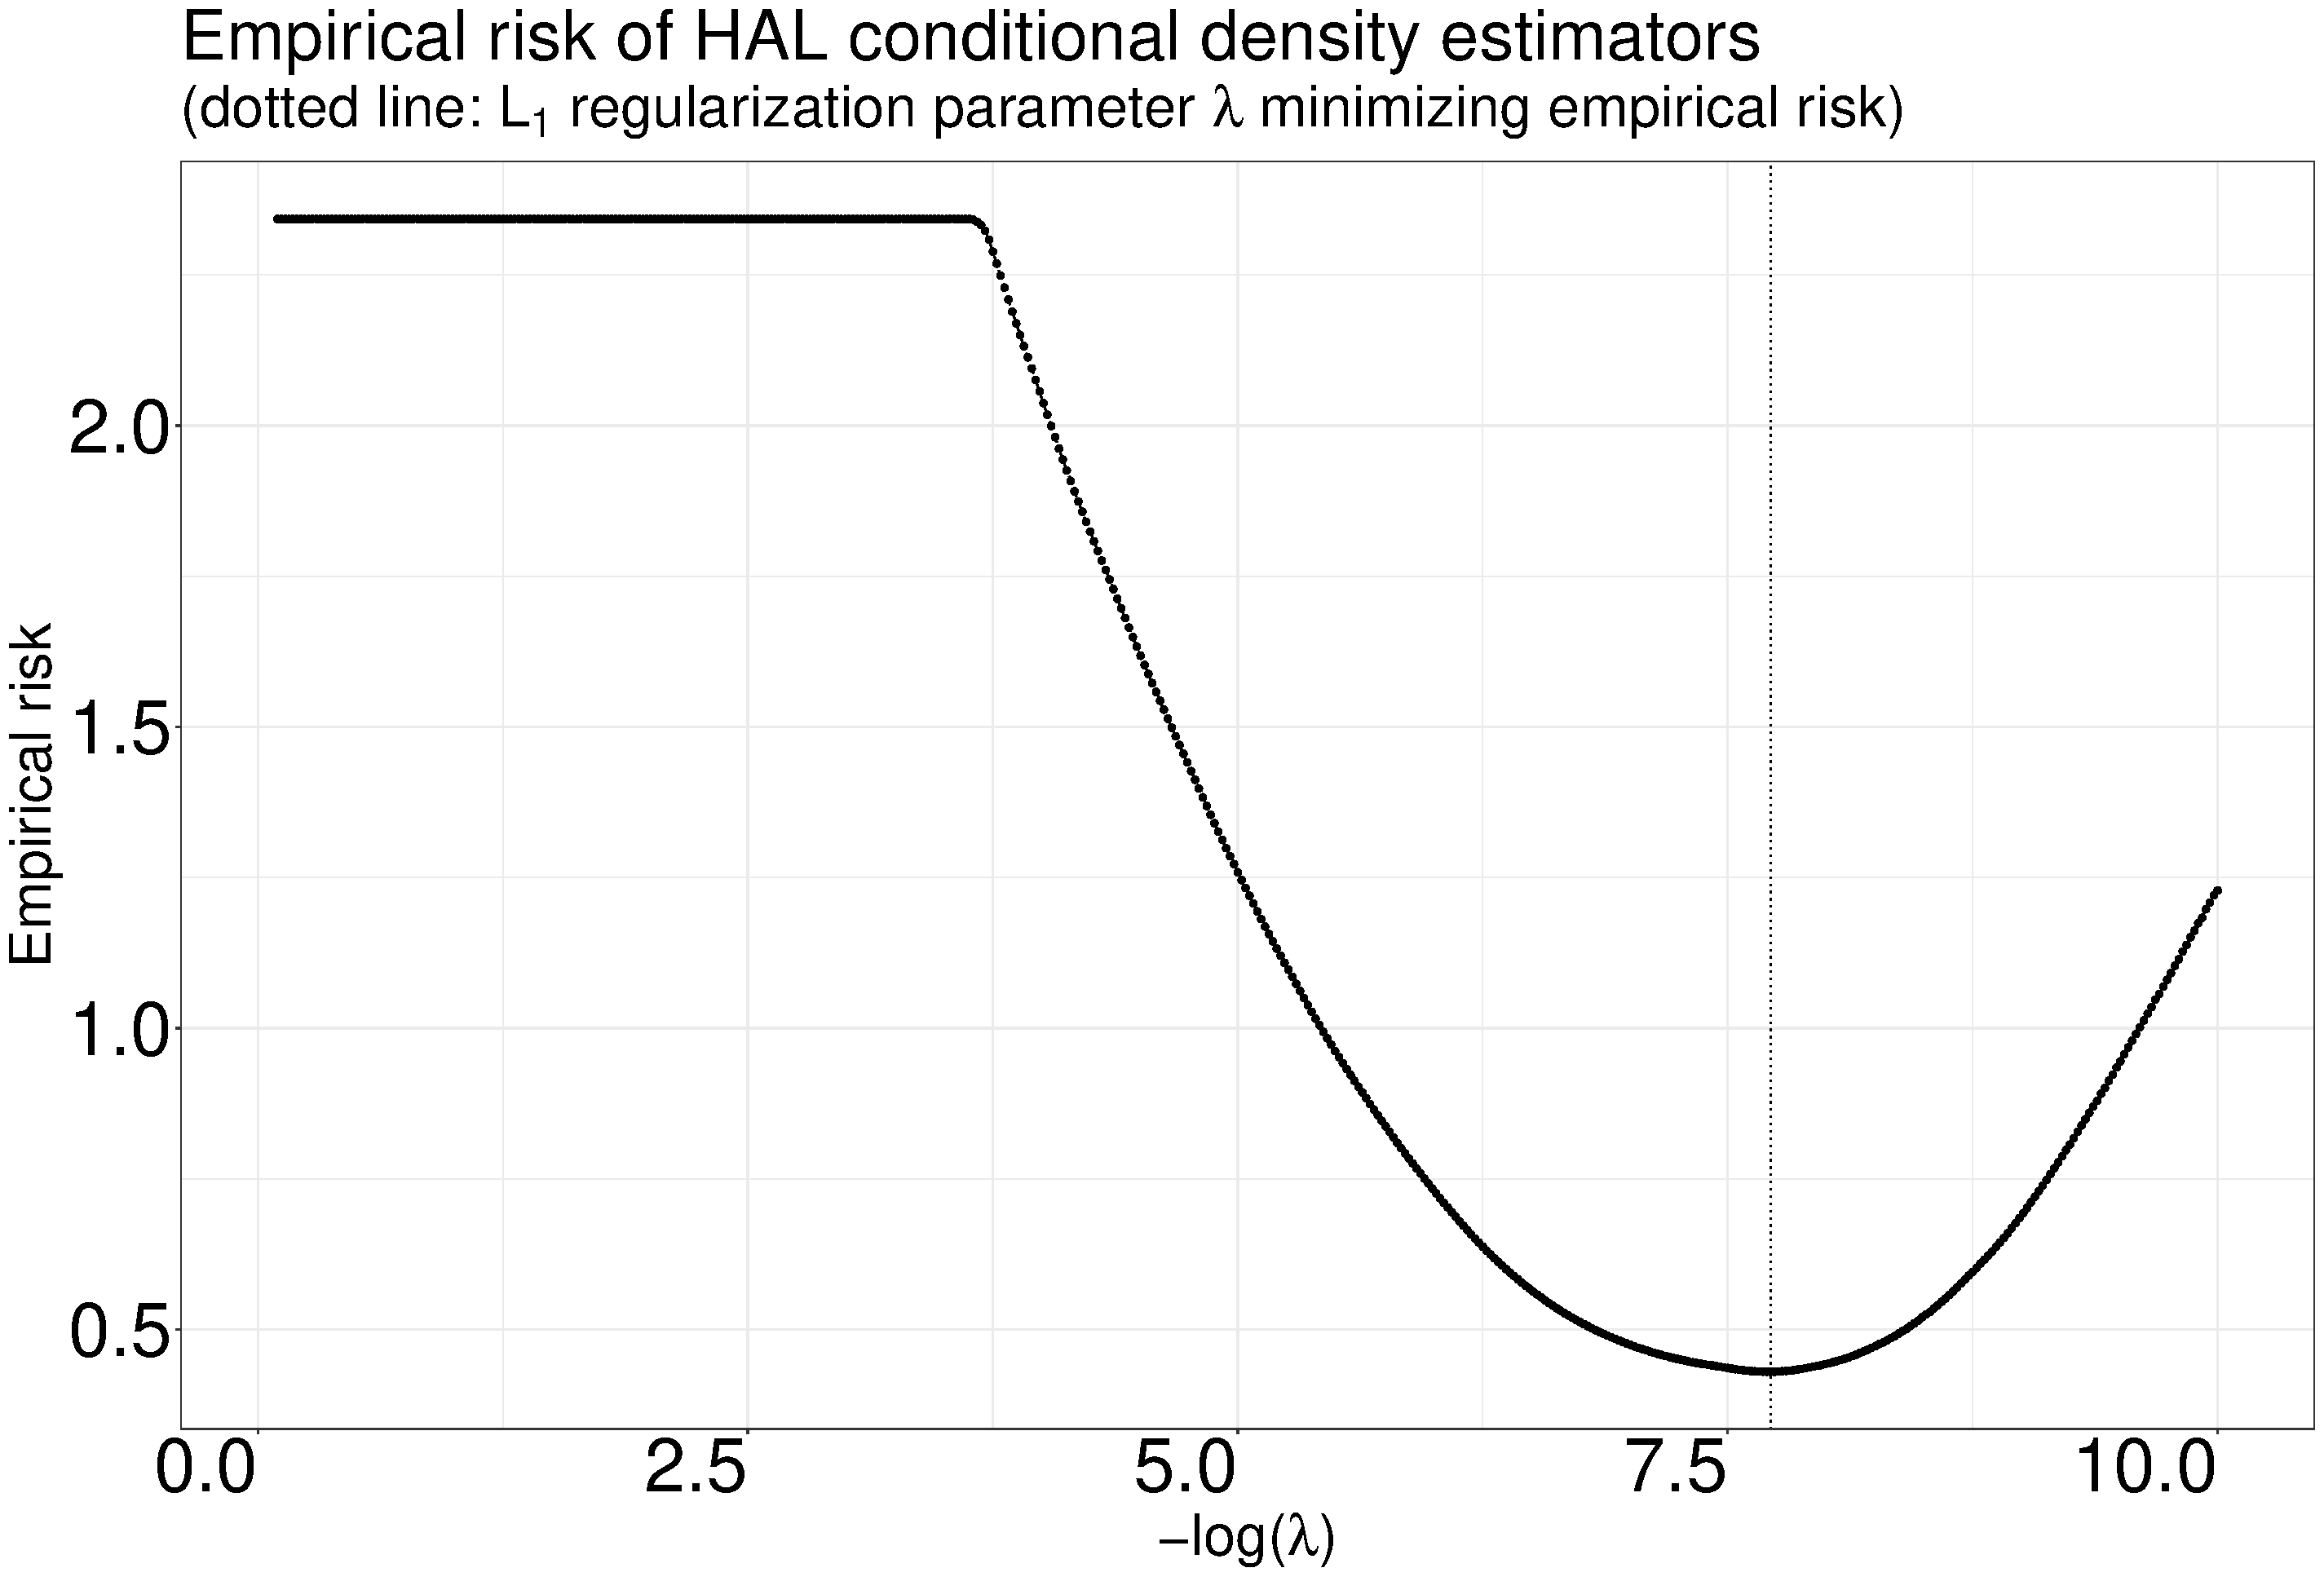
\includegraphics[scale=0.28]{haldensify_risk}
  \caption{Empirical risk of the estimated conditional density $g_{n,A}$ across
      a grid in the regularization parameter $\lambda$.}
  \label{fig:haldensify_risk}
\end{figure}

Finally, we can predict the conditional density over the grid of observed values
$A$ across different elements of the support $W$. We do this using the
\texttt{predict()} method of \texttt{haldensify} and plot the results below.

\begin{lstlisting}[language=R]
# predictions to recover conditional density of A|W
new_a <- seq(-4, 4, by = 0.05)
new_dat <- as.data.table(list(
  a = new_a,
  w_neg = rep(-2, length(new_a)),
  w_zero = rep(0, length(new_a)),
  w_pos = rep(2, length(new_a))
))
new_dat[, pred_w_neg := predict(haldensify_fit, new_A = new_dat[["a"]],
                                new_W = new_dat[["w_neg"]])]
new_dat[, pred_w_zero := predict(haldensify_fit, new_A = new_dat[["a"]],
                                 new_W = new_dat[["w_zero"]])]
new_dat[, pred_w_pos := predict(haldensify_fit, new_A = new_dat[["a"]],
                                new_W = new_dat[["w_pos"]])]

# visualize results
dens_dat <-  melt(
  new_dat,
  id = c("a"),
  measure.vars = c("pred_w_pos", "pred_w_zero", "pred_w_neg")
)
p_dens <- ggplot(dens_dat, aes(x = a, y = value, colour = variable)) +
  geom_point() +
  geom_line() +
  stat_function(fun = dnorm, args = list(mean = -2, sd = 0.25),
                colour = "blue", linetype = "dashed") +
  stat_function(fun = dnorm, args = list(mean = 0, sd = 0.25),
                colour = "darkgreen", linetype = "dashed") +
  stat_function(fun = dnorm, args = list(mean = 2, sd = 0.25),
                colour = "red", linetype = "dashed") +
  labs(
    x = "Observed value of W",
    y = "Estimated conditional density",
    title = "Conditional density estimates g(A|W)"
  ) +
  theme_bw() +
  theme(legend.position = "none")
p_dens
\end{lstlisting}

The resulting conditional density estimates are visualzed in
Figure~\ref{fig:haldensify_est}.
\begin{figure}[H]
  \centering
  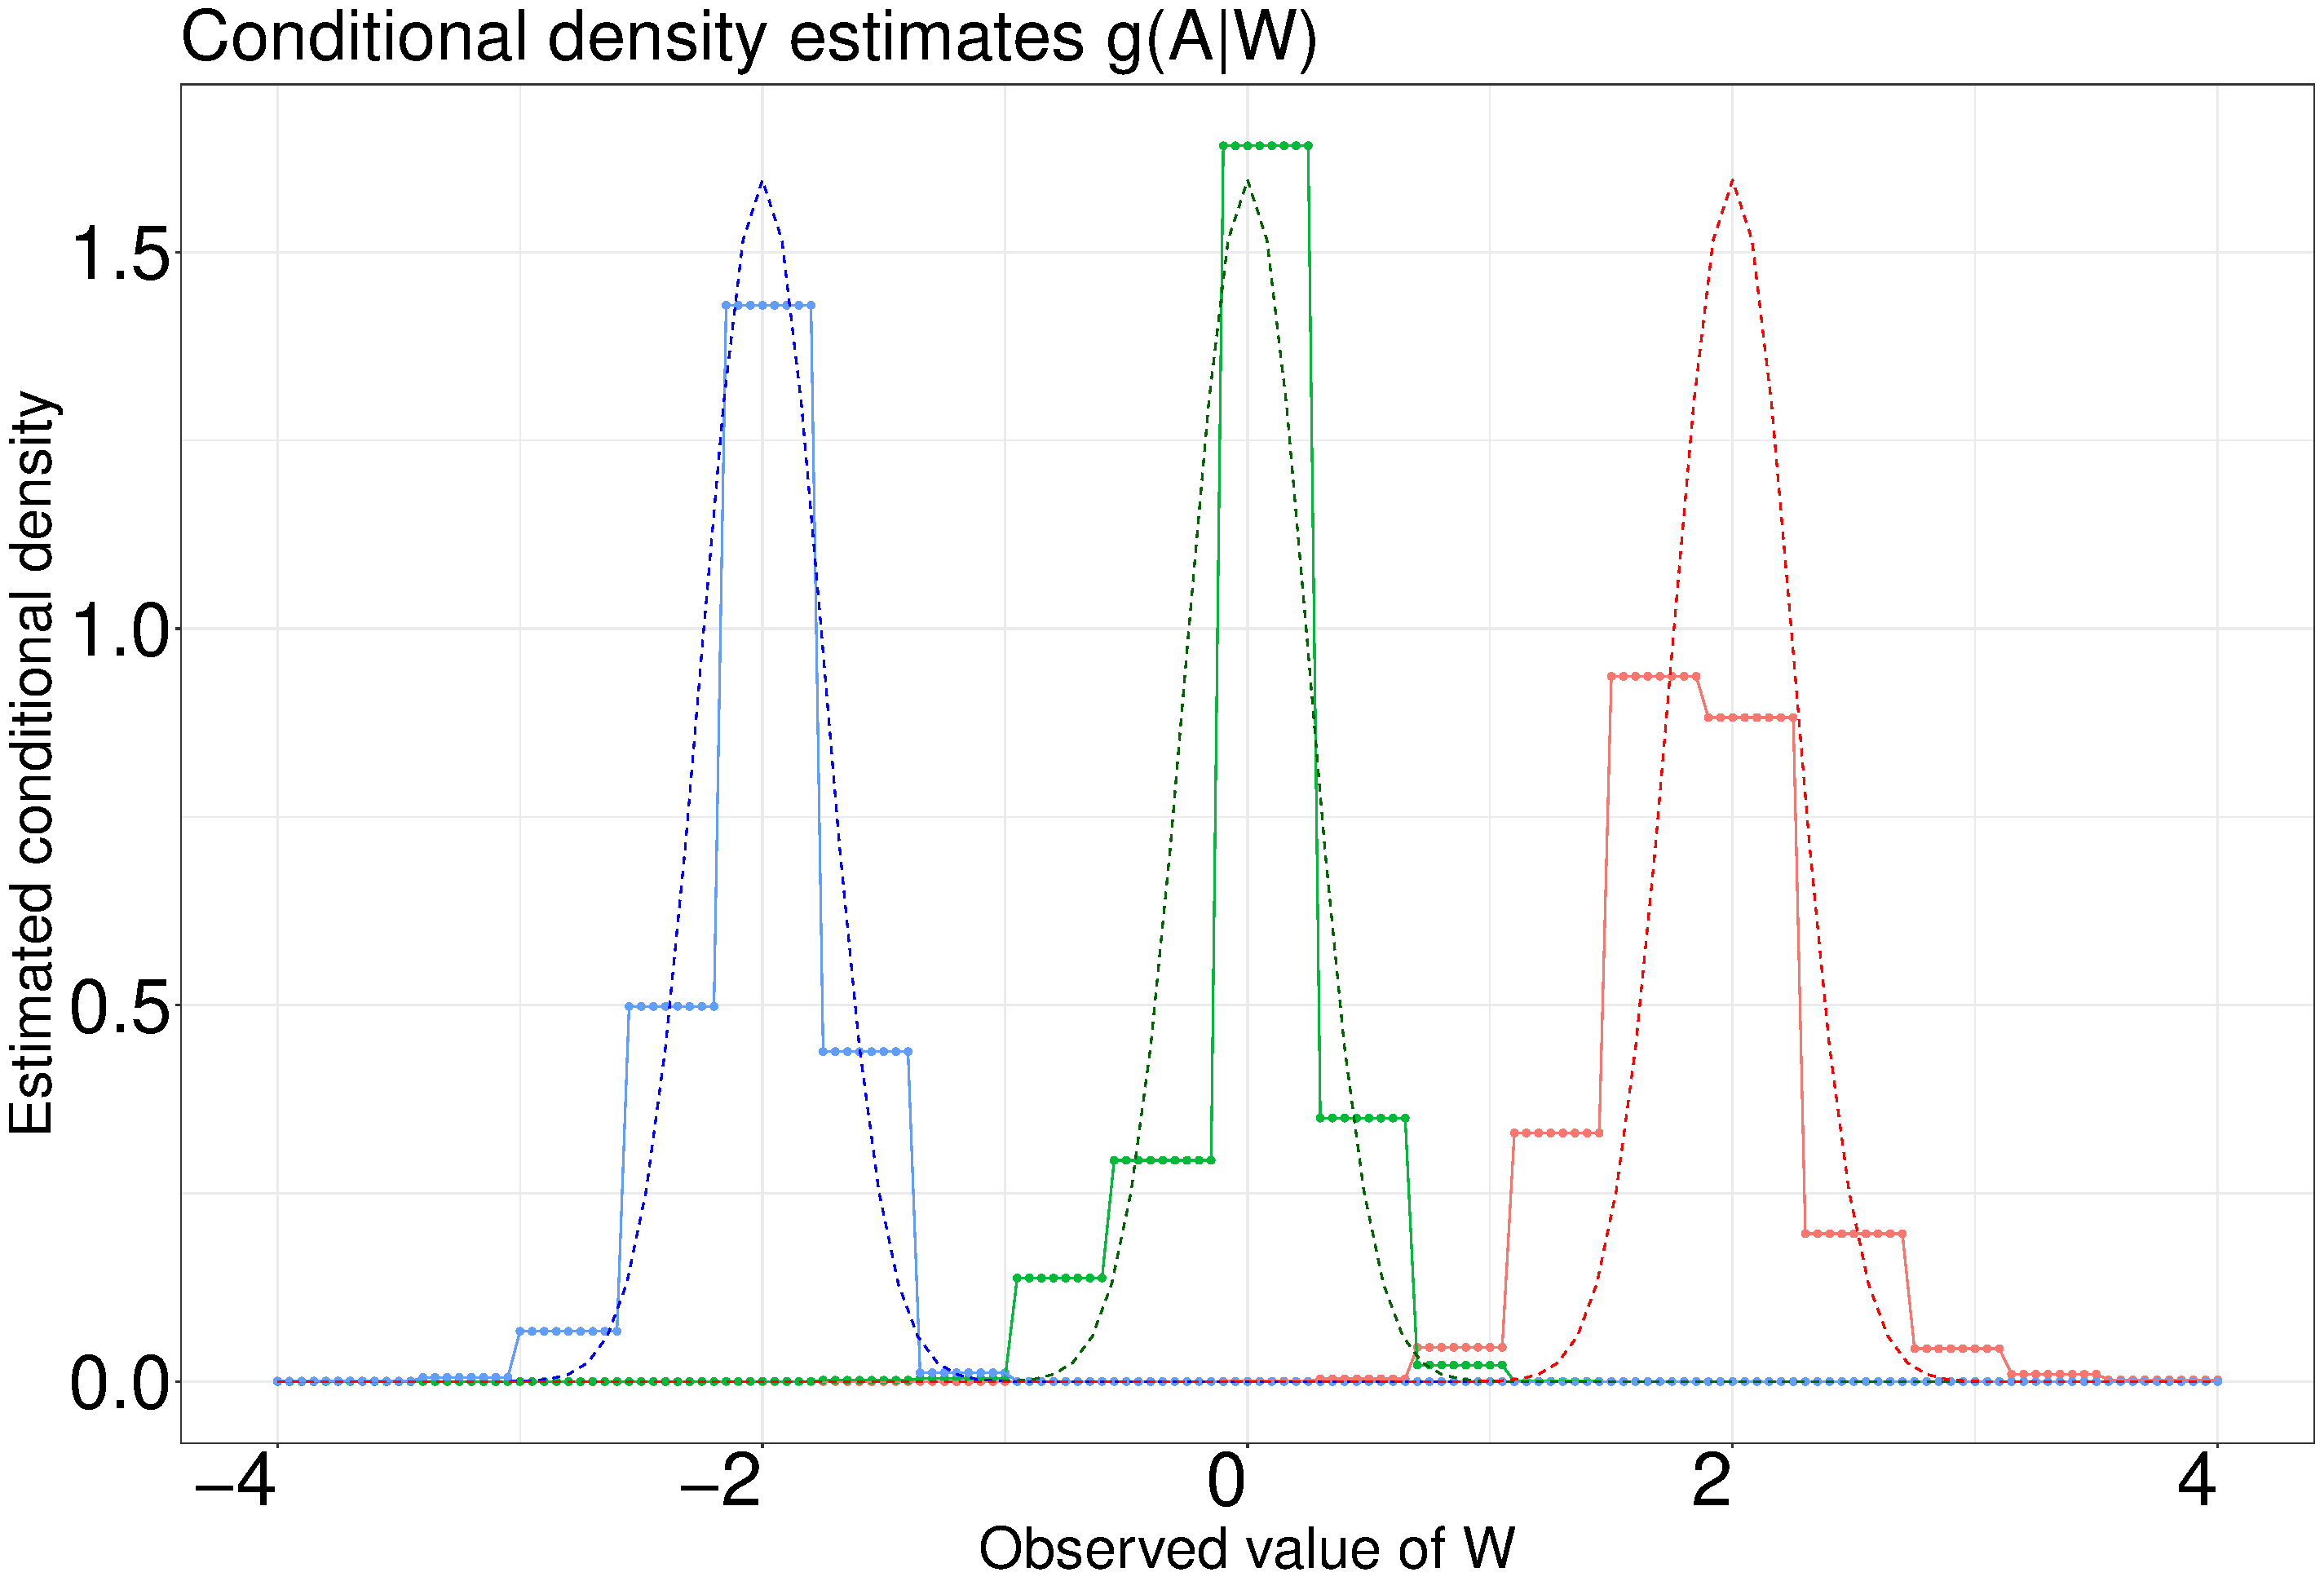
\includegraphics[scale=0.28]{haldensify_est}
  \caption{Conditional density estimates evaluated at different values of $W$,
    compared to the reference distribution at those same values.}
  \label{fig:haldensify_est}
\end{figure}


% \appendix
% \chapter{More Monticello Candidates}

\printbibliography

\end{document}
